\chapter{Mathematical Toolkit}\label{app:math}

Empirical industrial organization uses a small set of mathematical tools again and again. Pass-through formulas
come from the implicit function theorem, and Shephard's lemma and Roy's identity come from the envelope theorem.
Logit demand comes from the algebra of the Gumbel distribution. The identification of auction models comes from
the distribution theory of order statistics. This appendix states each tool with its assumptions, gives or locates
a proof, and shows how the chapters use it.

The appendix serves two kinds of reader. A reader who meets a tool in a chapter can come here for a precise
statement, a proof, a worked example and the usual pitfalls. A reader who wants a systematic treatment can read
the appendix from start to finish, because each section builds on the earlier ones. Several chapters prove a tool
in the context of one application. For those results we usually restate the theorem and refer to the chapter
that proves it. We give full proofs for the tools that no chapter proves and for the parts of a result that go
beyond the chapter's version. Worked applications, such as pass-through in \cref{sec:B-passthrough}, keep their
derivations because they show a tool at work.

The sections follow the logic of the tools. \Cref{sec:B-prelim} collects calculus, matrix and probability facts.
\Cref{sec:B-ift,sec:B-envelope} develop the two workhorses of comparative statics, the implicit function theorem
and the envelope theorem. \Cref{sec:B-duality} applies the envelope theorem to consumer and producer theory, and
\cref{sec:B-ev} derives the logit family from the extreme value distribution. \Cref{sec:B-orderstats} turns to
order statistics, the language of auction data. \Cref{sec:B-fixedpoint} treats fixed points: the inversion of
market shares, and the existence, uniqueness and computation of price equilibria. \Cref{sec:B-logconcave,%
sec:B-supermod} study the shape restrictions that make equilibria exist, comparative statics signable and auction
models tractable. These are log-concavity, supermodularity and affiliation. \Cref{tab:B-toolmap} maps each tool
to its section and to the chapters that use it.

Notation follows the rest of the book, with a few generic symbols. A generic parameter is $a \in A \subseteq \R^m$
and a generic choice is $x \in X \subseteq \R^n$. We never use $\theta$ for a generic parameter, because $\theta$
denotes conduct and $(\theta_1, \theta_2)$ denote demand parameters elsewhere. Euler's constant is $\gamma_E$, the
modulus of a contraction is $\kappa$, and the curvature of inverse demand is $\chi = -\frac{qP''}{P'}$, as in
\cref{ch:theory}. Symbols that matter in one section only are introduced there. In \cref{sec:B-duality}, for
instance, $I$ denotes income and $r$ a vector of input prices, while $r$ is a reserve price in the auction
applications.

\begin{table}[!tb]
\centering
\caption{The tools of this appendix and where the book uses them}\label{tab:B-toolmap}
\footnotesize
\renewcommand{\arraystretch}{1.3}
\begin{tabularx}{\textwidth}{@{}>{\raggedright\arraybackslash}p{2.6cm}>{\raggedright\arraybackslash}p{1.3cm}%
>{\raggedright\arraybackslash}p{4.1cm}>{\raggedright\arraybackslash}X@{}}
\toprule
Tool & Section & Main result & Where the book uses it \\
\midrule
Implicit function theorem & \ref{sec:B-ift} & $D_a x = -[D_x\Psi]^{-1}D_a\Psi$ (\cref{thm:B-ift}) &
  Pass-through (\cref{ch:theory,ch:conduct}), best-response slopes (\cref{ch:theory}), gradient of the share
  inversion (\cref{ch:blp}), merger price effects (\cref{ch:mergers}) \\
Envelope theorem & \ref{sec:B-envelope} & $V'(a) = f_a(x^*(a), a)$ (\cref{thm:B-envelope}) &
  Shephard's and Hotelling's lemmas (\cref{ch:intro,ch:aids}), entry and profits (\cref{ch:theory}), bidder rents
  and revenue equivalence (\cref{ch:auction-theory}) \\
Duality & \ref{sec:B-duality} & Shephard's lemma, Roy's identity, the Slutsky equation, virtual and shadow
  prices &
  Almost ideal demand system (\cref{ch:aids}), new goods (\cref{ch:newgoods}), cost functions (\cref{ch:conduct,%
  ch:airlines}) \\
Extreme value and logit algebra & \ref{sec:B-ev} & Max-stability, the log-sum $\ln\Lambda + \gamma_E$, GEV shares
  (\cref{prop:B-maxstable,prop:B-logsum,thm:B-gev}) &
  Logit, nested logit and random coefficients demand (\cref{ch:diffprod,ch:discrete,ch:logit,ch:blp}),
  applications (\cref{ch:airlines,ch:newgoods,ch:mergers}) \\
Order statistics & \ref{sec:B-orderstats} & $F_{(k:n)} = \phi_{k:n} \circ F$, competing risks
  (\cref{prop:B-os-cdf,prop:B-competing-risks}) &
  Equilibrium bids and revenues (\cref{ch:auction-theory}), identification of value distributions
  (\cref{ch:auction-empirics}) \\
Contraction mapping & \ref{sec:B-fixedpoint} & Unique fixed point and geometric convergence
  (\cref{thm:B-banach}) &
  Share inversion (\cref{ch:blp,ch:airlines,ch:mergers}), computation of equilibria (\cref{ch:diffprod,%
  ch:mergers}, \cref{app:problems}) \\
Log-concavity & \ref{sec:B-logconcave} & Preserved by products, marginals and integration
  (\cref{prop:B-lc-products,prop:B-lc-cdf,thm:B-prekopa}) &
  Monopoly pricing and pass-through (\cref{ch:theory,ch:conduct}), existence of price equilibrium
  (\cref{ch:diffprod}), auctions (\cref{ch:auction-theory,ch:auction-empirics}) \\
Supermodularity and affiliation & \ref{sec:B-supermod} & Topkis's theorem, supermodular games, MLRP and
  association (\cref{thm:B-topkis,thm:B-smgames,thm:B-association}) &
  Strategic complements (\cref{ch:theory,ch:mergers}), the vertical model (\cref{ch:discrete}), affiliated
  values (\cref{ch:auction-theory,ch:auction-empirics}) \\
\bottomrule
\end{tabularx}

\medskip
\begin{minipage}{\textwidth}
\footnotesize Notes: Each section states the general result. It proves the result, proves the case the book uses,
or refers to the chapter or source that proves it. The chapters listed carry the economic applications.
\end{minipage}
\end{table}

\section{Notation and analytical preliminaries}\label{sec:B-prelim}

This section collects the calculus, matrix and probability facts that the rest of the appendix uses. Each fact
comes with a short proof or a precise reference. We state the facts in the form in which the chapters apply
them, and we point to those applications as we go.

\subsection{Vectors, derivatives and norms}\label{sec:B-notation}

Vectors are columns unless they are rows of product characteristics, and $^\top$ denotes the transpose. For
$x, y \in \R^n$ we write $x \geq y$ if $x_k \geq y_k$ for every $k$, and $x \gg y$ if every inequality is strict.
The vector of ones is $\mathbf{1}$, the $k$-th unit vector is $e_k$, and the identity matrix is $I_n$, or $I$ when
the size is clear. The indicator function is $\indic\{\cdot\}$. The generic parameter $a$ and the generic choice $x$
follow the conventions stated at the start of the appendix.

Derivatives follow one convention. For a differentiable $f : \R^n \to \R$, the \emph{gradient} $\nabla f(x)$ is
the column vector with entries $\frac{\partial f}{\partial x_k}$. For a differentiable map
$\Psi : \R^n \times \R^m \to \R^n$, written $\Psi(x, a)$, the \emph{Jacobian} $D_x\Psi$ is the $n \times n$ matrix
with $(j, k)$ element $\frac{\partial \Psi_j}{\partial x_k}$. Similarly, $D_a\Psi$ is the $n \times m$ matrix with
$(j, l)$ element $\frac{\partial \Psi_j}{\partial a_l}$. Row $j$ of a Jacobian collects the derivatives of the
$j$-th equation. The \emph{Hessian} $D^2_{xx}f$ has $(k, l)$ element $\frac{\partial^2 f}{\partial x_k\,\partial x_l}$,
and $D^2_{xa}f$ has $(k, l)$ element $\frac{\partial^2 f}{\partial x_k\,\partial a_l}$. A function is $C^r$ if it has
continuous partial derivatives up to order $r$. The Hessian of a $C^2$ function is symmetric by Young's theorem.

The chain rule takes a compact matrix form. Suppose $x(a)$ is differentiable and $h(a) = \Psi(x(a), a)$. Let
$D_a x$ be the $n \times m$ matrix with $(k, l)$ element $\frac{\partial x_k}{\partial a_l}$. Then
\begin{equation}\label{eq:B-chain}
D_a h(a) = D_x\Psi\big(x(a), a\big)\, D_a x(a) + D_a\Psi\big(x(a), a\big).
\end{equation}
Element by element, \eqref{eq:B-chain} reads
$\frac{\partial h_j}{\partial a_l} = \sum_{k} \frac{\partial \Psi_j}{\partial x_k}\frac{\partial x_k}{\partial a_l} + \frac{\partial \Psi_j}{\partial a_l}$.

Two matrices of share derivatives recur in the book. For mean utilities $\delta = (\delta_1, \dots, \delta_J)^\top$, the
matrix $\frac{\partial s}{\partial \delta^\top}$ has $(j, k)$ element $\frac{\partial s_j}{\partial \delta_k}$. For prices,
the matrix $\Delta$ has $(j, k)$ element $\Delta_{jk} = \frac{\partial s_j}{\partial p_k}$. Both follow the Jacobian
convention, so row $j$ describes how product $j$'s share responds to every mean utility or every price.

The orientation of $\Delta$ matters in the multiproduct pricing condition. Firm $f$ owns the products in
$\mathcal{J}_f$ and earns $M\sum_{k \in \mathcal{J}_f}(p_k - mc_k)s_k(p)$, where $M$ is market size. After division
by $M$, the first-order condition for the price of product $j \in \mathcal{J}_f$ is
\begin{equation}\label{eq:B-foc-scalar}
s_j(p) + \sum_{k \in \mathcal{J}_f}(p_k - mc_k)\frac{\partial s_k}{\partial p_j}(p) = 0 .
\end{equation}
The derivative $\frac{\partial s_k}{\partial p_j}$ is the $(k, j)$ element of $\Delta$, which is the $(j, k)$ element of
$\Delta^\top$. Let $\Omega$ be the ownership matrix, with $\Omega_{jk} = 1$ if $j$ and $k$ have the same owner and
$\Omega_{jk} = 0$ otherwise. The \emph{Hadamard} (element-wise) \emph{product} of two matrices of the same size is
$(A \odot B)_{jk} = A_{jk}B_{jk}$. Row $j$ of $(\Omega \odot \Delta^\top)(p - mc)$ is then
\begin{equation*}
\big[(\Omega \odot \Delta^\top)(p - mc)\big]_j = \sum_{k = 1}^{J}\Omega_{jk}\frac{\partial s_k}{\partial p_j}(p_k - mc_k)
= \sum_{k \in \mathcal{J}_f}(p_k - mc_k)\frac{\partial s_k}{\partial p_j} ,
\end{equation*}
because $\Omega_{jk}$ keeps exactly the products of $j$'s owner. Stacking the $J$ conditions \eqref{eq:B-foc-scalar}
gives
\begin{equation}\label{eq:B-foc-matrix}
s(p) + \big(\Omega \odot \Delta(p)^\top\big)(p - mc) = 0 .
\end{equation}
With single-product firms, $\Omega = I$ and row $j$ reads $s_j + (p_j - mc_j)\frac{\partial s_j}{\partial p_j} = 0$.
Solving,
\begin{equation*}
p_j - mc_j = -s_j\Big(\frac{\partial s_j}{\partial p_j}\Big)^{-1} = \Big(-\frac{\partial \ln s_j}{\partial p_j}\Big)^{-1} ,
\end{equation*}
so the dollar markup is the inverse of the own semi-elasticity of demand. \Cref{sec:04-bertrand-matrix} develops
\eqref{eq:B-foc-matrix} in full.

\begin{remark}[Two errors in the matrix condition]\label{rem:B-hadamard}
The ordinary product $\Omega\Delta^\top$ has $(j, k)$ element $\sum_{l}\Omega_{jl}\frac{\partial s_k}{\partial p_l}$. This sum
adds up the effects on $s_k$ of every price that $j$'s owner sets, and it has no economic meaning. The second
error transposes $\Delta$. The matrix $\Omega \odot \Delta$ places $\frac{\partial s_j}{\partial p_k}$, the effect of a
sibling's price on $j$'s share, where the condition needs $\frac{\partial s_k}{\partial p_j}$. When utility is linear in
price, $\Delta$ is symmetric and this error is invisible. That is the case for the logit and for random
coefficients on price, where $\frac{\partial s_j}{\partial p_k} = \int \alpha_i s_{ij}s_{ik}\,\dd F(\nu_i)$ for $k \neq j$
(\cref{prop:08-derivs}). With the utility $\alpha\ln(y_i - p_j)$ of \citet{BerryLevinsohnPakes1995}, the marginal
utility of money $\frac{\alpha}{y_i - p_k}$ depends on the product. Then $\Delta$ is asymmetric, and a transposed
$\Delta$ produces wrong markups.
\end{remark}

Norms measure the size of vectors and matrices. The \emph{sup norm} of $x \in \R^n$ is $\|x\|_\infty = \max_k |x_k|$. A matrix $A$ inherits the \emph{induced norm}
\begin{equation*}
\|A\|_\infty = \sup_{x \neq 0}\frac{\|Ax\|_\infty}{\|x\|_\infty} .
\end{equation*}
By construction $\|Ax\|_\infty \leq \|A\|_\infty\|x\|_\infty$. Applying this twice gives
$\|ABx\|_\infty \leq \|A\|_\infty\|B\|_\infty\|x\|_\infty$, so $\|AB\|_\infty \leq \|A\|_\infty\|B\|_\infty$. We drop the
subscript $\infty$ when no confusion can arise.

\begin{lemma}[Row-sum formula]\label{lem:B-rowsum}
For every real $n \times m$ matrix $A$,
$\|A\|_\infty = \max_{j}\sum_{k}|A_{jk}|$.
\end{lemma}

\begin{proof}
Let $R = \max_j\sum_k|A_{jk}|$. For any $x$ and any row $j$,
\begin{equation*}
|(Ax)_j| = \Big|\sum_k A_{jk}x_k\Big| \leq \sum_k|A_{jk}|\,|x_k| \leq \Big(\sum_k|A_{jk}|\Big)\|x\|_\infty \leq R\,\|x\|_\infty .
\end{equation*}
Taking the maximum over $j$ gives $\|Ax\|_\infty \leq R\|x\|_\infty$, so $\|A\|_\infty \leq R$. For the reverse
inequality, let row $j^*$ attain the maximum. Set $x_k = 1$ if $A_{j^*k} \geq 0$ and $x_k = -1$ otherwise. Then
$\|x\|_\infty = 1$ and $(Ax)_{j^*} = \sum_k|A_{j^*k}| = R$, so $\|A\|_\infty \geq R$.
\end{proof}

The lemma turns a contraction property of a differentiable map into a condition on the row sums of its Jacobian
(\cref{prop:B-jacobian-criterion}). This is why the uniqueness conditions of \citet{Berry1994} and the contraction
conditions of \citet{BerryLevinsohnPakes1995} are both stated as row sums.

\subsection{Concavity, quasi-concavity and homogeneity}\label{sec:B-concavity}

\begin{definition}[Concave and quasi-concave functions]\label{def:B-concave}
Let $X \subseteq \R^n$ be convex and $f : X \to \R$. The function $f$ is \emph{concave} if
$f(\lambda x + (1 - \lambda)y) \geq \lambda f(x) + (1 - \lambda)f(y)$ for all $x, y \in X$ and $\lambda \in [0, 1]$.
It is \emph{strictly concave} if the inequality is strict whenever $x \neq y$ and $\lambda \in (0, 1)$. It is
\emph{convex} if $-f$ is concave. It is \emph{quasi-concave} if
$f(\lambda x + (1 - \lambda)y) \geq \min\{f(x), f(y)\}$, and \emph{strictly quasi-concave} if this inequality is
strict whenever $x \neq y$ and $\lambda \in (0, 1)$.
\end{definition}

Quasi-concavity is equivalent to convexity of every upper contour set $\{x \in X : f(x) \geq u\}$. Every concave
function is quasi-concave, since $\lambda f(x) + (1 - \lambda)f(y) \geq \min\{f(x), f(y)\}$. The converse fails, because
every monotone function of one variable is quasi-concave.

\begin{proposition}[Second-order characterization]\label{prop:B-concave-hessian}
Let $X$ be open and convex and $f \in C^2$ on $X$.
\begin{enumerate}[label=(\alph*)]
  \item The function $f$ is concave if and only if $D^2_{xx}f(x)$ is negative semidefinite at every $x \in X$.
  \item If $D^2_{xx}f(x)$ is negative definite at every $x \in X$, then $f$ is strictly concave.
\end{enumerate}
The converse of (b) fails.
\end{proposition}

\begin{proof}
A function is concave if and only if its restriction to every segment is concave. For $x \in X$ and a direction
$h$, let $g(t) = f(x + th)$ on the interval of $t$ for which $x + th \in X$. The chain rule gives
$g''(t) = h^\top D^2_{xx}f(x + th)\,h$. A $C^2$ function of one variable is concave if and only if $g' $ is
nonincreasing, that is, if and only if $g'' \leq 0$. So $f$ is concave if and only if $h^\top D^2_{xx}f\,h \leq 0$ for all
$x$ and $h$, which is (a). Under the hypothesis of (b), $g'' < 0$ for every $h \neq 0$. Then $g'$ is strictly
decreasing, $g$ is strictly concave, and so is $f$. The function $f(x) = -x^4$ is strictly concave, yet
$f''(0) = 0$.
\end{proof}

\begin{lemma}[First-order bound]\label{lem:B-concave-foc}
Let $f$ be differentiable and concave on an open convex set $X$. Then
$f(y) \leq f(x) + \nabla f(x)^\top(y - x)$ for all $x, y \in X$. In particular, a point $x^*$ with
$\nabla f(x^*) = 0$ maximizes $f$ on $X$.
\end{lemma}

\begin{proof}
For $\lambda \in (0, 1]$, concavity gives $f(x + \lambda(y - x)) \geq f(x) + \lambda[f(y) - f(x)]$. Rearranging,
\begin{equation*}
\frac{f(x + \lambda(y - x)) - f(x)}{\lambda} \geq f(y) - f(x) .
\end{equation*}
As $\lambda \to 0$ the left side converges to the directional derivative $\nabla f(x)^\top(y - x)$.
\end{proof}

\begin{lemma}[Minimum of affine functions]\label{lem:B-minlinear}
Let $Z$ be convex and let $\{\ell_x : x \in X\}$ be any family of affine functions $\ell_x(z) = b_x + c_x^\top z$ on
$Z$. If $g(z) = \inf_{x \in X}\ell_x(z)$ is finite on $Z$, then $g$ is concave. If
$\bar g(z) = \sup_{x \in X}\ell_x(z)$ is finite on $Z$, then $\bar g$ is convex.
\end{lemma}

\begin{proof}
Take $z, z' \in Z$ and $\lambda \in [0, 1]$. For every $x$, affinity and the definition of $g$ give
\begin{equation*}
\ell_x(\lambda z + (1 - \lambda)z') = \lambda\ell_x(z) + (1 - \lambda)\ell_x(z') \geq \lambda g(z) + (1 - \lambda)g(z') .
\end{equation*}
Taking the infimum over $x$ on the left gives $g(\lambda z + (1 - \lambda)z') \geq \lambda g(z) + (1 - \lambda)g(z')$. The
statement for $\bar g$ follows by applying the first one to the family $-\ell_x$.
\end{proof}

The lemma gives curvature properties of value functions without any differentiability. The expenditure function
$e(p, u) = \min_q\{p^\top q : U(q) \geq u\}$ is a minimum of functions that are linear in $p$, so it is concave in $p$
(\cref{sec:B-duality}). The cost function is concave in input prices for the same reason, and the profit function is
convex in prices because it is a maximum of linear functions (\cref{ex:B-hotelling}).

\begin{lemma}[Maximizers of quasi-concave functions]\label{lem:B-qc-argmax}
If $f$ is quasi-concave on a convex set $X$, its set of maximizers on $X$ is convex. If $f$ is strictly
quasi-concave, it has at most one maximizer.
\end{lemma}

\begin{proof}
Let $V^* = \max_{x \in X}f(x)$, and let $x$ and $y$ be maximizers. For $\lambda \in [0, 1]$, quasi-concavity gives
$f(\lambda x + (1 - \lambda)y) \geq \min\{f(x), f(y)\} = V^*$, so $\lambda x + (1 - \lambda)y$ is a maximizer. If $f$ is
strictly quasi-concave and $x \neq y$, the midpoint satisfies $f\big(\frac{1}{2}x + \frac{1}{2}y\big) > V^*$, which is
impossible.
\end{proof}

Best responses of a player with a quasi-concave payoff are therefore convex-valued. This is the property that
Kakutani's fixed-point theorem needs to deliver existence of a pricing equilibrium (\cref{thm:B-kakutani},
\cref{sec:B-logconcave}).

\begin{definition}[Homogeneity]\label{def:B-homogeneous}
A function $f$ defined on a cone $X \subseteq \R^n$ is \emph{homogeneous of degree $r$} if $f(tx) = t^rf(x)$ for
every $x \in X$ and every $t > 0$.
\end{definition}

\begin{proposition}[Euler's theorem]\label{prop:B-euler}
Let $f$ be differentiable and homogeneous of degree $r$ on an open cone. Then
\begin{enumerate}[label=(\alph*)]
  \item $\sum_{k = 1}^{n}x_k\frac{\partial f}{\partial x_k}(x) = r f(x)$ for every $x$, and
  \item every partial derivative $\frac{\partial f}{\partial x_k}$ is homogeneous of degree $r - 1$.
\end{enumerate}
\end{proposition}

\begin{proof}
Fix $x$ and differentiate the identity $f(tx) = t^rf(x)$ with respect to $t$:
\begin{equation*}
\sum_{k}x_k\frac{\partial f}{\partial x_k}(tx) = r t^{r - 1}f(x) .
\end{equation*}
Setting $t = 1$ gives (a). For (b), differentiate the same identity with respect to $x_k$:
\begin{equation*}
t\,\frac{\partial f}{\partial x_k}(tx) = t^r\frac{\partial f}{\partial x_k}(x) .
\end{equation*}
Dividing by $t$ gives $\frac{\partial f}{\partial x_k}(tx) = t^{r - 1}\frac{\partial f}{\partial x_k}(x)$.
\end{proof}

Euler's theorem produces the adding-up identities of demand theory (\cref{sec:B-duality}). The expenditure function
$e(p, u)$ is homogeneous of degree one in $p$, so $\sum_i p_i\frac{\partial e}{\partial p_i} = e$. Hicksian demand
$h(p, u)$ is homogeneous of degree zero in $p$, so $\sum_j p_j\frac{\partial h_i}{\partial p_j} = 0$, which says that the
Slutsky matrix annihilates the price vector. Marshallian demand $q_i(p, I)$ is homogeneous of degree zero in
$(p, I)$, so
\begin{equation*}
\sum_j p_j\frac{\partial q_i}{\partial p_j} + I\,\frac{\partial q_i}{\partial I} = 0 .
\end{equation*}
Dividing by $q_i$ turns this into the statement that price and income elasticities of each good sum to zero.

\begin{corollary}[Translation invariance]\label{cor:B-translation}
Let $f : \R^n \to \R$ be differentiable with $f(x + c\mathbf{1}) = f(x)$ for all $x$ and all $c \in \R$. Then
\begin{equation*}
\sum_{k = 1}^{n}\frac{\partial f}{\partial x_k}(x) = \nabla f(x)^\top\mathbf{1} = 0 .
\end{equation*}
\end{corollary}

\begin{proof}
The function $c \mapsto f(x + c\mathbf{1})$ is constant, so its derivative at $c = 0$ is zero. By the chain rule
that derivative is $\nabla f(x)^\top\mathbf{1}$.
\end{proof}

The corollary is Euler's theorem in disguise. With $y_k = e^{x_k}$, translation invariance of $f$ is homogeneity of
degree zero of $\tilde f(y) = f(\ln y_1, \dots, \ln y_n)$. Euler's theorem then gives
$0 = \sum_k y_k\frac{\partial \tilde f}{\partial y_k} = \sum_k\frac{\partial f}{\partial x_k}$.

\begin{example}[Shares depend only on utility differences]\label{ex:B-translation-shares}
In an additive random utility model, consumer $i$ obtains $\delta_k + \epsilon_{ik}$ from alternative
$k = 0, 1, \dots, J$. Adding the same constant to every $\delta_k$, the outside good's $\delta_0$ included, leaves
every consumer's choice unchanged. Hence $s_j(\delta + c\mathbf{1}) = s_j(\delta)$ for $\delta = (\delta_0, \dots, \delta_J)$,
and \cref{cor:B-translation} gives
\begin{equation}\label{eq:B-translation-shares}
\sum_{k = 0}^{J}\frac{\partial s_j}{\partial \delta_k} = 0 .
\end{equation}
If the outside good is a substitute for $j$, so that $\frac{\partial s_j}{\partial \delta_0} < 0$, then
\begin{equation*}
\sum_{k = 1}^{J}\frac{\partial s_j}{\partial \delta_k} = -\frac{\partial s_j}{\partial \delta_0} > 0 .
\end{equation*}
This is the step on which \citet[p.~261]{Berry1994} builds his uniqueness argument (\cref{ex:B-share-dd}). In the
logit, $\frac{\partial s_j}{\partial \delta_k} = s_j(\indic\{j = k\} - s_k)$ for $k = 0, \dots, J$, and the sum in
\eqref{eq:B-translation-shares} is $s_j\big(1 - \sum_{k = 0}^{J}s_k\big) = 0$.
\end{example}

\subsection{Mean values, integrals and transformations of random variables}\label{sec:B-calculus}

The scalar mean value theorem says that a function differentiable on $(u, u')$ and continuous on $[u, u']$
satisfies $g(u') - g(u) = g'(\tau)(u' - u)$ for some $\tau \in (u, u')$. For vector-valued maps there is no single
intermediate point, and the right tool is an integral.

\begin{proposition}[Integral form of the mean value theorem]\label{prop:B-mvt-integral}
Let $U \subseteq \R^d$ be open, let $\Psi : U \to \R^n$ be $C^1$, and suppose the segment
$[x, x'] = \{x + t(x' - x) : t \in [0, 1]\}$ lies in $U$. Then
\begin{equation}\label{eq:B-mvt-integral}
\Psi(x') - \Psi(x) = \Big[\int_0^1 D\Psi\big(x + t(x' - x)\big)\,\dd t\Big](x' - x) ,
\end{equation}
where the integral of a matrix is taken element by element.
\end{proposition}

\begin{proof}
For each $j$, the function $g_j(t) = \Psi_j(x + t(x' - x))$ is $C^1$ on $[0, 1]$. The chain rule gives
\begin{equation*}
g_j'(t) = \sum_{k}\frac{\partial \Psi_j}{\partial x_k}\big(x + t(x' - x)\big)(x'_k - x_k) .
\end{equation*}
By the fundamental theorem of calculus, $\Psi_j(x') - \Psi_j(x) = g_j(1) - g_j(0) = \int_0^1 g_j'(t)\,\dd t$. Stacking
the $n$ rows gives \eqref{eq:B-mvt-integral}.
\end{proof}

A single intermediate point does not exist in general. The map $\Psi(t) = (\cos t, \sin t)^\top$ satisfies
$\Psi(2\pi) - \Psi(0) = 0$, while its derivative $(-\sin t, \cos t)^\top$ never vanishes.

\begin{corollary}[Mean value inequality]\label{cor:B-mvi}
Under the assumptions of \cref{prop:B-mvt-integral},
\begin{equation*}
\|\Psi(x') - \Psi(x)\|_\infty \leq \sup_{z \in [x, x']}\|D\Psi(z)\|_\infty\;\|x' - x\|_\infty .
\end{equation*}
\end{corollary}

\begin{proof}
Write $z_t = x + t(x' - x)$. Row $j$ of \eqref{eq:B-mvt-integral} gives
\begin{equation*}
|\Psi_j(x') - \Psi_j(x)| \leq \int_0^1\sum_k\Big|\frac{\partial \Psi_j}{\partial x_k}(z_t)\Big|\,|x'_k - x_k|\,\dd t
\leq \int_0^1\sum_k\Big|\frac{\partial \Psi_j}{\partial x_k}(z_t)\Big|\,\dd t\;\|x' - x\|_\infty .
\end{equation*}
By \cref{lem:B-rowsum} the row sum inside the integral is at most $\|D\Psi(z_t)\|_\infty$. Bounding it by the
supremum over the segment and maximizing over $j$ gives the claim.
\end{proof}

\begin{example}[The mean value step in the BLP contraction]\label{ex:B-blp-mvt}
\citet[Appendix I, p.~887]{BerryLevinsohnPakes1995} study a $C^1$ map $f : \R^J \to \R^J$ whose partial derivatives
are nonnegative and whose row sums $\sum_k\frac{\partial f_j}{\partial x_k}$ are below one. Their operator is
$f(\delta) = \delta + \ln s^{obs} - \ln s(\delta)$, equation (6.8) on p.~865. Take two points $x, x'$ in a bounded box
and let $\lambda = \|x - x'\|_\infty$, so that $x' \leq x + \lambda\mathbf{1}$. Suppose $f_j(x') \geq f_j(x)$. Monotonicity
and \eqref{eq:B-mvt-integral} along the direction $\mathbf{1}$ give
\begin{equation*}
f_j(x') - f_j(x) \leq f_j(x + \lambda\mathbf{1}) - f_j(x)
= \int_0^\lambda\Big[\sum_{k = 1}^{J}\frac{\partial f_j}{\partial x_k}(x + z\mathbf{1})\Big]\dd z \leq \kappa\lambda ,
\end{equation*}
where $\kappa < 1$ is the largest row sum over the compact set of points that the segments can reach. The same bound
follows from \cref{cor:B-mvi}, because with nonnegative partials $\|Df\|_\infty$ is the largest row sum. This step makes
the truncated map a contraction. The full theorem and its proof are in \cref{thm:08-contraction}.
\end{example}

\begin{proposition}[Leibniz's rule]\label{prop:B-leibniz}
\begin{enumerate}[label=(\alph*)]
  \item Let $g(x, a)$ and $g_a(x, a) = \frac{\partial g}{\partial a}(x, a)$ be continuous on
  $[x_L, x_U] \times [a_L, a_U]$, and let $l(a)$ and $m(a)$ be differentiable with values in $[x_L, x_U]$. Then
  $\Gamma(a) = \int_{l(a)}^{m(a)}g(x, a)\,\dd x$ satisfies, for $a \in (a_L, a_U)$,
  \begin{equation}\label{eq:B-leibniz}
  \Gamma'(a) = g\big(m(a), a\big)m'(a) - g\big(l(a), a\big)l'(a) + \int_{l(a)}^{m(a)}g_a(x, a)\,\dd x .
  \end{equation}
  \item Let $\mu$ be a measure, such as the distribution $F$ of a taste shock. Suppose $g(\cdot, a)$ is
  $\mu$-integrable for each $a$ in an open interval $N$ and that $g_a(x, a)$ exists there. Suppose also that an
  integrable function $b(x)$ satisfies $|g_a(x, a)| \leq b(x)$ for all $x$ and all $a \in N$. Then for $a \in N$,
  \begin{equation*}
  \frac{\dd}{\dd a}\int g(x, a)\,\dd\mu(x) = \int g_a(x, a)\,\dd\mu(x) .
  \end{equation*}
\end{enumerate}
\end{proposition}

\begin{proof}
We prove (b) first. For $h \neq 0$ small, the scalar mean value theorem gives
$\frac{g(x, a + h) - g(x, a)}{h} = g_a(x, a + \tau_x h)$ for some $\tau_x \in (0, 1)$. This difference quotient is
bounded by $b(x)$, and it converges to $g_a(x, a)$ as $h \to 0$. Dominated convergence lets us pass the limit
through the integral.

For (a), define $G(u, w, a) = \int_w^u g(x, a)\,\dd x$. The fundamental theorem of calculus gives
$\frac{\partial G}{\partial u} = g(u, a)$ and $\frac{\partial G}{\partial w} = -g(w, a)$. Part (b), with $\mu$ the Lebesgue
measure on $[x_L, x_U]$ and $b$ the maximum of $|g_a|$ on the compact rectangle, gives
$\frac{\partial G}{\partial a} = \int_w^u g_a(x, a)\,\dd x$. These partial derivatives are continuous, so $G$ is $C^1$. The
chain rule applied to $\Gamma(a) = G(m(a), l(a), a)$ gives \eqref{eq:B-leibniz}.
\end{proof}

\begin{example}[Share derivatives with random coefficients]\label{ex:B-rc-derivatives}
In the random coefficients logit, consumer $i$ with taste draw $\nu_i$ buys $j$ with probability
$s_{ij}(p, \nu_i) = \frac{\exp(\delta_j + \mu_{ij})}{1 + \sum_{k}\exp(\delta_k + \mu_{ik})}$. Her price coefficient is $\alpha_i$, so
$\frac{\partial(\delta_k + \mu_{ik})}{\partial p_k} = -\alpha_i$. The logit derivative
$\frac{\partial s_{ij}}{\partial(\delta_k + \mu_{ik})} = s_{ij}(\indic\{j = k\} - s_{ik})$ and the chain rule give
\begin{equation*}
\frac{\partial s_{ij}}{\partial p_k} = \alpha_i\, s_{ij}\big(s_{ik} - \indic\{j = k\}\big) .
\end{equation*}
Market shares are $s_j(p) = \int s_{ij}(p, \nu)\,\dd F(\nu)$. Because shares lie in $[0, 1]$, the integrand's derivative
satisfies $|\alpha_i s_{ij}(s_{ik} - \indic\{j = k\})| \leq |\alpha_i|$ at every price vector. If $\E|\alpha_i| < \infty$,
\cref{prop:B-leibniz}(b) applies with $b = |\alpha_i|$ and
\begin{equation}\label{eq:B-rc-derivative}
\frac{\partial s_j}{\partial p_k} = \int \alpha_i\, s_{ij}\big(s_{ik} - \indic\{j = k\}\big)\,\dd F(\nu_i) .
\end{equation}
With $B$ simulation draws the integral becomes an average over draws (\cref{prop:08-derivs}).
\end{example}

A second application has a variable limit of integration. In first-price auctions with $n$ bidders, values drawn
from $F$, and reserve price $r$, the function $\int_r^v F(t)^{n - 1}\,\dd t$ has derivative $F(v)^{n - 1}$ by
\eqref{eq:B-leibniz} with $l' = 0$, $m(v) = v$ and $g_a = 0$. \Cref{ex:B-auction-envelope} uses this step, and
\cref{sec:B-orderstats} uses Leibniz's rule to derive the densities of order statistics.

\begin{lemma}[Tail formula for the mean]\label{lem:B-tail}
If $X \geq 0$ has CDF $F$, then $\E[X] = \int_0^\infty\big(1 - F(x)\big)\,\dd x$, where both sides may be infinite.
\end{lemma}

\begin{proof}
Write $X = \int_0^\infty\indic\{x < X\}\,\dd x$. Take expectations and exchange the order of integration, which
Tonelli's theorem allows because the integrand is nonnegative:
\begin{equation*}
\E[X] = \int_0^\infty\E\big[\indic\{x < X\}\big]\,\dd x = \int_0^\infty\Pr(X > x)\,\dd x = \int_0^\infty\big(1 - F(x)\big)\,\dd x .
\qedhere
\end{equation*}
\end{proof}

The same exchange of integrals is integration by parts,
$\int_u^{u'}\varphi\,\dd\psi = \varphi(u')\psi(u') - \varphi(u)\psi(u) - \int_u^{u'}\psi\,\dd\varphi$, in probabilistic form. Auction
theory uses it to write bids as conditional expectations.

\begin{example}[The first-price bid as a conditional expectation]\label{ex:B-rs-parts}
Let $Y_1$ be the highest of $n - 1$ rival values, drawn independently from $F$, so its CDF is $F^{n - 1}$. For $v > r$,
consider $\E[\max\{Y_1, r\} \mid Y_1 < v]$. The event $Y_1 \leq r$ has probability $F(r)^{n - 1}$ and contributes $r$, so
\begin{equation*}
\E[\max\{Y_1, r\} \mid Y_1 < v] = \frac{rF(r)^{n - 1} + \int_r^v t\,\dd\big[F(t)^{n - 1}\big]}{F(v)^{n - 1}} .
\end{equation*}
Integration by parts with $\varphi(t) = t$ and $\psi(t) = F(t)^{n - 1}$ gives
\begin{equation*}
\int_r^v t\,\dd\big[F(t)^{n - 1}\big] = vF(v)^{n - 1} - rF(r)^{n - 1} - \int_r^vF(t)^{n - 1}\,\dd t .
\end{equation*}
The boundary terms in $r$ cancel, and
\begin{equation}\label{eq:B-rs-bid}
\E[\max\{Y_1, r\} \mid Y_1 < v] = v - \frac{\int_r^v F(t)^{n - 1}\,\dd t}{F(v)^{n - 1}} .
\end{equation}
The right side is the equilibrium bid of the symmetric first-price auction \citep{RileySamuelson1981}, derived in
\cref{ex:B-auction-envelope} and in \cref{sec:14-fpa-envelope}.
\end{example}

\begin{lemma}[Probability integral transform]\label{lem:B-pit}
\begin{enumerate}[label=(\alph*)]
  \item If $X$ has a continuous CDF $F$, then $F(X)$ is uniformly distributed on $[0, 1]$.
  \item For any CDF $F$, define the generalized inverse $F^{-1}(u) = \inf\{x : F(x) \geq u\}$ for $u \in (0, 1)$. If
  $U$ is uniform on $[0, 1]$, then $F^{-1}(U)$ has CDF $F$.
\end{enumerate}
\end{lemma}

\begin{proof}
Right continuity of $F$ implies that $F^{-1}(u) \leq x$ if and only if $u \leq F(x)$. For (b),
$\Pr(F^{-1}(U) \leq x) = \Pr(U \leq F(x)) = F(x)$. For (a), fix $u \in (0, 1)$. The same equivalence shows that
$F(X) \geq u$ if and only if $X \geq F^{-1}(u)$. Continuity of $F$ gives $\Pr(X \geq x) = 1 - F(x)$ and
$F(F^{-1}(u)) = u$. Hence
\begin{equation*}
\Pr\big(F(X) \geq u\big) = \Pr\big(X \geq F^{-1}(u)\big) = 1 - F\big(F^{-1}(u)\big) = 1 - u ,
\end{equation*}
so $\Pr(F(X) < u) = u$ for every $u \in (0, 1)$, which is the uniform distribution.
\end{proof}

Part (b) is how simulation draws are produced. The standard Gumbel CDF $\exp(-e^{-x})$ has inverse
$-\ln(-\ln u)$, so $-\ln(-\ln U)$ is a standard Gumbel draw (\cref{sec:B-ev}). Part (a) maps order statistics of any
continuous distribution into order statistics of uniforms (\cref{sec:B-orderstats}).

\subsection{Matrix facts}\label{sec:B-matrix}

A symmetric matrix $A$ is \emph{negative semidefinite} if $x^\top Ax \leq 0$ for every $x$, and \emph{negative definite}
if $x^\top Ax < 0$ for every $x \neq 0$. Equivalently, all eigenvalues of $A$ are nonpositive in the first case and
negative in the second. Positive
(semi)definiteness is defined with the inequalities reversed. Second-order conditions for maximization and the
negativity of the Slutsky matrix (\cref{sec:B-duality}) are statements of this kind. In practice they are checked
with determinants.

\begin{proposition}[Principal minors]\label{prop:B-minors}
Let $A$ be a symmetric $n \times n$ matrix and let $A_k$ be its leading $k \times k$ submatrix.
\begin{enumerate}[label=(\alph*)]
  \item $A$ is negative definite if and only if $(-1)^k\det A_k > 0$ for $k = 1, \dots, n$.
  \item $A$ is negative semidefinite if and only if $(-1)^k\det A_S \geq 0$ for every principal submatrix $A_S$ of
  order $k$, formed from any $k$ rows and the same $k$ columns, for every $k$.
\end{enumerate}
\end{proposition}

\Citet{SimonBlume1994} prove both parts. For $n = 2$, part (a) says that $\begin{psmallmatrix} a_{11} & a_{12} \\ a_{12} & a_{22}\end{psmallmatrix}$ is
negative definite if and only if $a_{11} < 0$ and $a_{11}a_{22} - a_{12}^2 > 0$. Part (b) needs every principal minor,
including those that are not leading. The matrix $\begin{psmallmatrix} 0 & 0 \\ 0 & 1\end{psmallmatrix}$ has leading minors $0$ and $0$, which
satisfy the weak sign conditions. Yet it is not negative semidefinite, and its principal minor of order one in the
second position equals $1$.

\begin{lemma}[Diagonal dominance]\label{lem:B-dd}
Let $A$ be a real $n \times n$ matrix.
\begin{enumerate}[label=(\alph*)]
  \item (Gershgorin) Every eigenvalue $z$ of $A$, real or complex, satisfies
  $|A_{jj} - z| \leq \sum_{k \neq j}|A_{jk}|$ for at least one row $j$.
  \item (Levy-Desplanques) If $A$ is \emph{strictly diagonally dominant}, that is,
  $|A_{jj}| > \sum_{k \neq j}|A_{jk}|$ for every row $j$, then $A$ is nonsingular.
  \item If $A$ is symmetric, strictly diagonally dominant and has a negative diagonal, then $A$ is negative definite.
\end{enumerate}
\end{lemma}

\begin{proof}
For (a), let $Ax = zx$ with $x \neq 0$, and pick $j$ with $|x_j| = \|x\|_\infty > 0$. Row $j$ of the eigenvalue equation
reads $(A_{jj} - z)x_j = -\sum_{k \neq j}A_{jk}x_k$. Taking absolute values and dividing by $|x_j|$,
\begin{equation*}
|A_{jj} - z| \leq \sum_{k \neq j}|A_{jk}|\,\frac{|x_k|}{|x_j|} \leq \sum_{k \neq j}|A_{jk}| .
\end{equation*}
For (b), $z = 0$ would require $|A_{jj}| \leq \sum_{k \neq j}|A_{jk}|$ for some row, which strict dominance rules
out. So $0$ is not an eigenvalue and $A$ is nonsingular. For (c), the eigenvalues of a symmetric matrix are real.
By (a) each lies within $\sum_{k \neq j}|A_{jk}| < |A_{jj}| = -A_{jj}$ of some $A_{jj} < 0$, so each is negative.
\end{proof}

\begin{example}[The share Jacobian is invertible]\label{ex:B-share-dd}
Assume, with \citet[p.~260]{Berry1994}, that $\frac{\partial s_j}{\partial \delta_j} > 0$ and
$\frac{\partial s_j}{\partial \delta_k} < 0$ for every $k \neq j$, the outside good included. By
\cref{ex:B-translation-shares},
\begin{equation*}
\frac{\partial s_j}{\partial \delta_j} - \sum_{k \geq 1, k \neq j}\Big|\frac{\partial s_j}{\partial \delta_k}\Big|
= \sum_{k = 1}^{J}\frac{\partial s_j}{\partial \delta_k} = -\frac{\partial s_j}{\partial \delta_0} > 0 .
\end{equation*}
So the $J \times J$ matrix $\frac{\partial s}{\partial \delta^\top}$ of inside goods is strictly diagonally dominant at every
$\delta$. By \cref{lem:B-dd} it is nonsingular. This is Berry's condition (A2), and in the logit the margin of
dominance is $s_js_0$. The implicit function theorem then delivers the derivatives of the inverse share function
(\cref{ex:B-inversion-gradient}).
\end{example}

\begin{lemma}[Neumann series]\label{lem:B-neumann}
Let $\|\cdot\|$ be an induced matrix norm and $\|A\| < 1$. Then $I - A$ is nonsingular,
\begin{equation*}
(I - A)^{-1} = \sum_{h = 0}^{\infty}A^h , \qquad\text{and}\qquad \big\|(I - A)^{-1}\big\| \leq \frac{1}{1 - \|A\|} .
\end{equation*}
\end{lemma}

\begin{proof}
Let $S_H = \sum_{h = 0}^{H}A^h$. Submultiplicativity gives $\|A^h\| \leq \|A\|^h$, so for $H' > H$,
\begin{equation*}
\|S_{H'} - S_H\| \leq \sum_{h = H + 1}^{H'}\|A\|^h \leq \frac{\|A\|^{H + 1}}{1 - \|A\|} \to 0 .
\end{equation*}
The partial sums are therefore Cauchy and converge to a matrix $S$. Telescoping gives
$(I - A)S_H = I - A^{H + 1}$, and $A^{H + 1} \to 0$. Taking limits, $(I - A)S = I$, and $S(I - A) = I$ in the same
way. The bound follows from $\|S_H\| \leq \sum_{h \leq H}\|A\|^h \leq \frac{1}{1 - \|A\|}$.
\end{proof}

The lemma is the linear case of the contraction mapping theorem (\cref{thm:B-banach}). The affine map
$\Phi(x) = Ax + b$ contracts with modulus $\|A\|$, and its iterates from $x^{(0)} = 0$ are $x^{(H)} = S_{H - 1}b$. They
converge to the fixed point $(I - A)^{-1}b$. \Cref{prop:B-cs-nash} reads the series as rounds of strategic responses.

\begin{lemma}[Sherman-Morrison formula]\label{lem:B-sm}
Let $B$ be nonsingular and $u, v$ vectors with $1 - v^\top B^{-1}u \neq 0$. Then
\begin{equation}\label{eq:B-sm}
\big(B - uv^\top\big)^{-1} = B^{-1} + \frac{B^{-1}uv^\top B^{-1}}{1 - v^\top B^{-1}u} .
\end{equation}
\end{lemma}

\begin{proof}
Write $\tau = 1 - v^\top B^{-1}u$ and multiply $B - uv^\top$ by the right side of \eqref{eq:B-sm}:
\begin{align*}
\big(B - uv^\top\big)\Big(B^{-1} + \frac{B^{-1}uv^\top B^{-1}}{\tau}\Big)
&= I + \frac{uv^\top B^{-1}}{\tau} - uv^\top B^{-1} - \frac{u\,(v^\top B^{-1}u)\,v^\top B^{-1}}{\tau} \\
&= I + uv^\top B^{-1}\,\frac{1 - \tau - v^\top B^{-1}u}{\tau} = I ,
\end{align*}
because $1 - \tau = v^\top B^{-1}u$. The scalar $v^\top B^{-1}u$ can be moved in front of $v^\top B^{-1}$ because it
is a number.
\end{proof}

\begin{example}[The logit Jacobian, its inverse, and logit markups]\label{ex:B-logit-jacobian}
In the logit, $s_j = \frac{e^{\delta_j}}{\Lambda}$ with $\Lambda = 1 + \sum_{k = 1}^{J}e^{\delta_k}$ and $s_0 = \frac{1}{\Lambda}$. Since
$\frac{\partial \Lambda}{\partial \delta_k} = e^{\delta_k}$, the quotient rule gives
\begin{equation*}
\frac{\partial s_j}{\partial \delta_j} = \frac{e^{\delta_j}\Lambda - e^{\delta_j}e^{\delta_j}}{\Lambda^2} = s_j(1 - s_j) ,
\qquad
\frac{\partial s_j}{\partial \delta_k} = -\frac{e^{\delta_j}e^{\delta_k}}{\Lambda^2} = -s_js_k \quad (k \neq j) .
\end{equation*}
In matrix form, with $s = (s_1, \dots, s_J)^\top$,
\begin{equation}\label{eq:B-logit-jacobian}
\frac{\partial s}{\partial \delta^\top} = \diag(s) - ss^\top .
\end{equation}
This is a diagonal matrix minus a rank-one matrix, so \cref{lem:B-sm} applies with $B = \diag(s)$ and $u = v = s$.
Two facts do the work:
\begin{equation*}
\diag(s)^{-1}s = \mathbf{1} , \qquad s^\top\diag(s)^{-1}s = s^\top\mathbf{1} = \sum_{k = 1}^{J}s_k = 1 - s_0 .
\end{equation*}
The denominator in \eqref{eq:B-sm} is $1 - (1 - s_0) = s_0 > 0$, and the numerator is $\mathbf{1}\mathbf{1}^\top$. Hence
\begin{equation}\label{eq:B-logit-jacobian-inverse}
\big[\diag(s) - ss^\top\big]^{-1} = \diag\Big(\frac{1}{s_1}, \dots, \frac{1}{s_J}\Big) + \frac{1}{s_0}\mathbf{1}\mathbf{1}^\top .
\end{equation}
A direct check confirms \eqref{eq:B-logit-jacobian-inverse}. The logit inversion $\delta_j = \ln s_j - \ln s_0$ with
$s_0 = 1 - \sum_k s_k$ has $\frac{\partial \delta_j}{\partial s_k} = \frac{\indic\{j = k\}}{s_j} + \frac{1}{s_0}$, which is the
$(j, k)$ element of \eqref{eq:B-logit-jacobian-inverse}, as the inverse function theorem requires.

Markups follow in a few lines. With $\delta_j = \tilde\delta_j - \alpha p_j$, the price Jacobian is
$\Delta = -\alpha\big[\diag(s) - ss^\top\big]$, which is symmetric. Write $m = p - mc$, so \eqref{eq:B-foc-matrix} gives
$m = -(\Omega \odot \Delta^\top)^{-1}s$.
\begin{enumerate}[label=(\roman*)]
  \item Single-product firms. With $\Omega = I$, the matrix $\Omega \odot \Delta^\top$ is diagonal with entries
  $-\alpha s_j(1 - s_j)$. Hence $m_j = \frac{s_j}{\alpha s_j(1 - s_j)} = \frac{1}{\alpha(1 - s_j)}$.
  \item One owner of all inside goods. With $\Omega = \mathbf{1}\mathbf{1}^\top$, we have $\Omega \odot \Delta^\top = \Delta$, and
  \eqref{eq:B-logit-jacobian-inverse} gives
  \begin{equation*}
  m = \frac{1}{\alpha}\Big[\diag\Big(\frac{1}{s_1}, \dots, \frac{1}{s_J}\Big) + \frac{1}{s_0}\mathbf{1}\mathbf{1}^\top\Big]s
  = \frac{1}{\alpha}\Big[\mathbf{1} + \frac{1 - s_0}{s_0}\mathbf{1}\Big] = \frac{1}{\alpha s_0}\mathbf{1} .
  \end{equation*}
  Every product carries the same markup $\frac{1}{\alpha s_0}$.
  \item A multiproduct firm. Order products by owner, so that $\Omega$ is block diagonal. Then $\Omega \odot \Delta^\top$ is
  block diagonal with blocks $-\alpha\big[\diag(s_f) - s_fs_f^\top\big]$, where $s_f$ collects the shares of firm $f$.
  \Cref{lem:B-sm} with $v^\top B^{-1}u = \sum_{k \in \mathcal{J}_f}s_k \equiv S_f$ inverts each block as
  $\diag(s_f)^{-1} + \frac{1}{1 - S_f}\mathbf{1}\mathbf{1}^\top$. The same computation as in (ii) gives the common markup
  \begin{equation*}
  m_k = \frac{1}{\alpha}\Big[1 + \frac{S_f}{1 - S_f}\Big] = \frac{1}{\alpha(1 - S_f)} \qquad\text{for every } k \in \mathcal{J}_f .
  \end{equation*}
\end{enumerate}
Case (iii) contains (i) with $S_f = s_j$ and (ii) with $S_f = 1 - s_0$. \Cref{prop:04-logit-markup} derives the same
formula from the scalar conditions, and \cref{sec:B-logit-algebra} reuses the example.
\end{example}

\section{The implicit function theorem and comparative statics}\label{sec:B-ift}

Equilibrium conditions rarely solve for the endogenous variables in closed form. First-order conditions,
market-clearing conditions and share equations define prices, quantities or mean utilities only implicitly, as
solutions $x$ of a system $\Psi(x, a) = 0$. Yet we need to know how the solution moves with costs, taxes, ownership
or demand parameters. The implicit function theorem says when the solution is a differentiable function $x(a)$,
and it gives the derivative without solving the system.

\subsection{Statement and proof}\label{sec:B-ift-statement}

\begin{theorem}[Implicit function theorem, scalar case]\label{thm:B-ift-scalar}
Let $\Psi : \R \times \R^m \to \R$ be $C^1$ near $(x_0, a_0)$, with $\Psi(x_0, a_0) = 0$ and $\Psi_x(x_0, a_0) \neq 0$.
Then there are open neighborhoods $N_a$ of $a_0$ and $N_x$ of $x_0$, and a unique function $x : N_a \to N_x$, such that
$\Psi(x(a), a) = 0$ for every $a \in N_a$. The function $x(\cdot)$ is $C^1$, and
\begin{equation}\label{eq:B-ift-scalar}
\frac{\partial x}{\partial a_l}(a) = -\frac{\Psi_{a_l}\big(x(a), a\big)}{\Psi_x\big(x(a), a\big)} , \qquad l = 1, \dots, m .
\end{equation}
\end{theorem}

\begin{proof}
We proceed in five steps.
\begin{enumerate}[label=Step \arabic*., leftmargin=*, align=left]
  \item Replacing $\Psi$ by $-\Psi$ if necessary, assume $\Psi_x(x_0, a_0) > 0$. By continuity of $\Psi_x$ there are
  $\epsilon > 0$ and $\eta > 0$ with $\Psi_x(x, a) > 0$ whenever $|x - x_0| \leq \epsilon$ and $\|a - a_0\| \leq \eta$. For
  each such $a$, the function $\Psi(\cdot, a)$ is strictly increasing on $[x_0 - \epsilon, x_0 + \epsilon]$.
  \item Since $\Psi(x_0, a_0) = 0$ and $\Psi(\cdot, a_0)$ is strictly increasing,
  $\Psi(x_0 - \epsilon, a_0) < 0 < \Psi(x_0 + \epsilon, a_0)$. By continuity of $\Psi$ in $a$, there is $\eta' \in (0, \eta]$
  such that $\Psi(x_0 - \epsilon, a) < 0 < \Psi(x_0 + \epsilon, a)$ for all $\|a - a_0\| < \eta'$.
  \item Let $N_a = \{a : \|a - a_0\| < \eta'\}$ and $N_x = (x_0 - \epsilon, x_0 + \epsilon)$. For $a \in N_a$, the intermediate
  value theorem gives a root $x(a) \in N_x$. Strict monotonicity makes it the only root in $N_x$.
  \item The function $x(\cdot)$ is continuous. At any $a_1 \in N_a$, repeat Steps 1 to 3 around $(x(a_1), a_1)$ with an
  arbitrary $\epsilon' > 0$ in place of $\epsilon$. For $a$ close enough to $a_1$, the unique root then lies within
  $\epsilon'$ of $x(a_1)$.
  \item Fix $a \in N_a$ and $l$, let $a' = a + h e_l$, and write $\Delta x = x(a') - x(a)$. Apply the scalar mean value
  theorem to $\tau \mapsto \Psi(x(a) + \tau\Delta x, a + \tau h e_l)$ on $[0, 1]$. Since $\Psi$ vanishes at both ends,
  \begin{equation*}
  0 = \Psi(x(a'), a') - \Psi(x(a), a) = \Psi_x(\xi)\,\Delta x + \Psi_{a_l}(\xi)\,h
  \end{equation*}
  for a point $\xi$ on the segment between $(x(a), a)$ and $(x(a'), a')$. Hence
  $\frac{\Delta x}{h} = -\frac{\Psi_{a_l}(\xi)}{\Psi_x(\xi)}$. As $h \to 0$, Step 4 gives $\Delta x \to 0$, so
  $\xi \to (x(a), a)$. Continuity of the partial derivatives yields \eqref{eq:B-ift-scalar}. The right side of
  \eqref{eq:B-ift-scalar} is continuous in $a$, so $x(\cdot)$ is $C^1$. \qedhere
\end{enumerate}
\end{proof}

\Cref{fig:B-ift} illustrates the theorem with $\Psi(x, a) = x^2 + a^2 - 1$, whose zero set is the unit circle. Here
$\Psi_x = 2x$ and $\Psi_a = 2a$. At $(a_0, x_0) = (0.6, 0.8)$ we have $\Psi_x = 1.6 \neq 0$. The theorem gives the
local solution $x(a) = \sqrt{1 - a^2}$ with slope
\begin{equation*}
x'(a_0) = -\frac{\Psi_a}{\Psi_x} = -\frac{2a_0}{2x_0} = -\frac{3}{4} ,
\end{equation*}
which matches the direct derivative $-\frac{a_0}{\sqrt{1 - a_0^2}}$. At $(1, 0)$, by contrast, $\Psi_x = 0$. In every box
around that point there are two solutions $\pm\sqrt{1 - a^2}$ for $a$ slightly below one and none for $a > 1$.

\begin{figure}[htbp]
\centering
\begin{tikzpicture}[x=2.3cm, y=2.3cm, >=Stealth]
  \draw[->] (-1.3,0) -- (1.55,0) node[right] {$a$};
  \draw[->] (0,-1.25) -- (0,1.35) node[above] {$x$};
  \draw[thick, black!45] (0,0) circle (1);
  \node[black!70, font=\small] at (-0.95,0.9) {$x^2 + a^2 = 1$};
  \draw[dashed, blue!60!black] (0.38,0.52) rectangle (0.84,1.04);
  \draw[very thick, blue!60!black, domain=0.38:0.84, samples=40, variable=\t] plot ({\t},{sqrt(1-\t*\t)});
  \draw[red!70!black, thick] (0.2,1.1) -- (1.05,0.4625);
  \fill[blue!60!black] (0.6,0.8) circle (0.022);
  \draw[->, black!70] (1.12,0.98) -- (0.64,0.82);
  \node[anchor=west, font=\small, align=left] at (1.12,1.02) {regular point $(a_0, x_0) = (0.6, 0.8)$,\\ unique local solution $x(a)$};
  \draw[->, black!70] (1.12,0.62) -- (0.93,0.56);
  \node[anchor=west, font=\small] at (1.12,0.62) {tangent with slope $-\frac{a_0}{x_0} = -\frac{3}{4}$};
  \draw[dashed, orange!80!black] (0.8,-0.36) rectangle (1.22,0.36);
  \draw[very thick, orange!80!black, domain=0.9367:1, samples=30, variable=\t] plot ({\t},{sqrt(1-\t*\t)});
  \draw[very thick, orange!80!black, domain=0.9367:1, samples=30, variable=\t] plot ({\t},{-sqrt(1-\t*\t)});
  \fill[orange!80!black] (1,0) circle (0.022);
  \draw[->, black!70] (1.3,-0.3) -- (1.03,-0.03);
  \node[anchor=west, font=\small, align=left] at (1.3,-0.38) {fold point $(1, 0)$, where $\Psi_x = 2x = 0$,\\ two solutions for $a < 1$, none for $a > 1$};
\end{tikzpicture}
\caption{The implicit function theorem for $\Psi(x, a) = x^2 + a^2 - 1$. Near the regular point $(0.6, 0.8)$ the zero set is
the graph of a unique $C^1$ function, whose slope $-\frac{\Psi_a}{\Psi_x} = -\frac{3}{4}$ is the slope of the tangent. Near the fold
point $(1, 0)$, where $\Psi_x = 0$, no box contains the graph of a unique function of $a$.}
\label{fig:B-ift}
\end{figure}

\begin{theorem}[Implicit function theorem]\label{thm:B-ift}
Let $\Psi : U \to \R^n$ be $C^1$ on an open set $U \subseteq \R^n \times \R^m$. Let $(x_0, a_0) \in U$ satisfy
$\Psi(x_0, a_0) = 0$, with $D_x\Psi(x_0, a_0)$ nonsingular. Then there are $\epsilon > 0$ and $\eta > 0$ with the following
property. For every $a$ with $\|a - a_0\| < \eta$, the system $\Psi(x, a) = 0$ has exactly one solution $x(a)$ with
$\|x(a) - x_0\| \leq \epsilon$. The function $x(\cdot)$ is $C^1$, and
\begin{equation}\label{eq:B-ift}
D_a x(a) = -\big[D_x\Psi\big(x(a), a\big)\big]^{-1}D_a\Psi\big(x(a), a\big) .
\end{equation}
\end{theorem}

\begin{proof}
All norms are sup norms and their induced matrix norms. We first derive \eqref{eq:B-ift} assuming that a
differentiable solution exists, and then prove existence, uniqueness and differentiability.

\emph{The derivative formula.} The function $h(a) = \Psi(x(a), a)$ is identically zero, so its Jacobian is zero. By
the chain rule \eqref{eq:B-chain},
\begin{align*}
0 &= D_a h(a) \\
  &= D_x\Psi\big(x(a), a\big)\,D_a x(a) + D_a\Psi\big(x(a), a\big) .
\end{align*}
Moving the second term to the left and premultiplying by $[D_x\Psi]^{-1}$ gives \eqref{eq:B-ift}.

\emph{Existence and uniqueness.} Let $J_0 = D_x\Psi(x_0, a_0)$ and define
\begin{equation*}
\Phi_a(x) = x - J_0^{-1}\Psi(x, a) .
\end{equation*}
Since $J_0^{-1}$ is nonsingular, $x$ is a fixed point of $\Phi_a$ exactly when $\Psi(x, a) = 0$. The Jacobian of $\Phi_a$ is
\begin{equation*}
D\Phi_a(x) = I - J_0^{-1}D_x\Psi(x, a) = J_0^{-1}\big[J_0 - D_x\Psi(x, a)\big] ,
\end{equation*}
which vanishes at $(x_0, a_0)$. By continuity of $D_x\Psi$, choose $\epsilon > 0$ and $\eta_1 > 0$ such that
$\|D\Phi_a(x)\| \leq \frac{1}{2}$ whenever $\|x - x_0\| \leq \epsilon$ and $\|a - a_0\| \leq \eta_1$. On the closed ball
$B_\epsilon = \{x : \|x - x_0\| \leq \epsilon\}$, which is convex, \cref{cor:B-mvi} gives
\begin{equation}\label{eq:B-ift-contraction}
\|\Phi_a(x) - \Phi_a(x')\| \leq \frac{1}{2}\|x - x'\| \qquad\text{for all } x, x' \in B_\epsilon .
\end{equation}
The map also sends $B_\epsilon$ into itself for $a$ close to $a_0$. For $x \in B_\epsilon$,
\begin{equation*}
\|\Phi_a(x) - x_0\| \leq \|\Phi_a(x) - \Phi_a(x_0)\| + \|\Phi_a(x_0) - x_0\| \leq \frac{\epsilon}{2} + \big\|J_0^{-1}\Psi(x_0, a)\big\| .
\end{equation*}
The last term is zero at $a = a_0$ and continuous in $a$. So there is $\eta \in (0, \eta_1]$ with
$\|J_0^{-1}\Psi(x_0, a)\| \leq \frac{\epsilon}{2}$ for $\|a - a_0\| < \eta$. For such $a$, $\Phi_a$ maps the complete set
$B_\epsilon$ into itself and contracts with modulus $\frac{1}{2}$. The contraction mapping theorem (\cref{thm:B-banach}) gives a
unique fixed point $x(a) \in B_\epsilon$.

\emph{Continuity.} For two parameter values $a, a'$, add and subtract $\Phi_a(x(a'))$ and use
\eqref{eq:B-ift-contraction}:
\begin{equation*}
\|x(a) - x(a')\| \leq \frac{1}{2}\|x(a) - x(a')\| + \big\|J_0^{-1}\big[\Psi(x(a'), a) - \Psi(x(a'), a')\big]\big\| .
\end{equation*}
Hence $\|x(a) - x(a')\| \leq 2\|J_0^{-1}\|\,\sup_{y \in B_\epsilon}\|\Psi(y, a) - \Psi(y, a')\|$. The supremum vanishes as $a' \to a$,
because $\Psi$ is uniformly continuous on compact sets.

\emph{Differentiability.} Fix $a$, write $x = x(a)$ and $x' = x(a')$, and let $z_t$ be the point
$(x + t(x' - x), a + t(a' - a))$. \Cref{prop:B-mvt-integral}, applied to $\Psi$ as a function of the stacked vector
$(x, a)$, gives
\begin{equation*}
0 = \Psi(x', a') - \Psi(x, a) = M_x\,(x' - x) + M_a\,(a' - a) ,
\end{equation*}
where $M_x = \int_0^1 D_x\Psi(z_t)\,\dd t$ and $M_a = \int_0^1 D_a\Psi(z_t)\,\dd t$.
The points $z_t$ stay in the region where $\|I - J_0^{-1}D_x\Psi\| \leq \frac{1}{2}$, so
$\|I - J_0^{-1}M_x\| \leq \frac{1}{2}$. \Cref{lem:B-neumann} makes $J_0^{-1}M_x$, and hence $M_x$, nonsingular. Therefore
$x' - x = -M_x^{-1}M_a(a' - a)$. As $a' \to a$, continuity gives $x' \to x$, $M_x \to D_x\Psi(x, a)$ and
$M_a \to D_a\Psi(x, a)$. So $x(\cdot)$ is differentiable with derivative \eqref{eq:B-ift}, which is continuous in $a$.
\end{proof}

\begin{remark}[The theorem is local]\label{rem:B-ift-local}
The theorem guarantees a unique solution only near $(x_0, a_0)$. It says nothing about solutions far from $x_0$.
Several price equilibria, for instance, can each be locally unique, with a nonsingular Jacobian at each one. Global
uniqueness needs other tools, such as contractions or dominant-diagonal conditions (\cref{sec:B-fixedpoint}). The
theorem also fails where $D_x\Psi$ is singular. At such fold points a small change in $a$ can make solutions
appear, disappear or jump, as at $(1, 0)$ in \cref{fig:B-ift}.
\end{remark}

\subsection{Comparative statics of optima and equilibria}\label{sec:B-cs-optimum}

\begin{proposition}[Comparative statics of an optimum]\label{prop:B-cs-optimum}
Let $f(x, a)$ be $C^2$ with $x$ in an open set $X \subseteq \R^n$. Suppose $x_0$ is an interior maximizer at $a_0$ with
$\nabla_x f(x_0, a_0) = 0$ and $D^2_{xx}f(x_0, a_0)$ negative definite. Then near $a_0$ there is a $C^1$ function
$x^*(a)$ of strict local maximizers with $x^*(a_0) = x_0$, and
\begin{equation}\label{eq:B-cs-optimum}
D_a x^*(a) = -\big[D^2_{xx}f(x^*(a), a)\big]^{-1}D^2_{xa}f(x^*(a), a) .
\end{equation}
In the scalar case $\frac{\dd x^*}{\dd a} = -\frac{f_{xa}}{f_{xx}}$, which has the sign of the cross partial $f_{xa}$.
\end{proposition}

\begin{proof}
Apply \cref{thm:B-ift} to $\Psi(x, a) = \nabla_x f(x, a)$. Its Jacobian $D_x\Psi = D^2_{xx}f$ is negative definite, hence
nonsingular, and $D_a\Psi = D^2_{xa}f$. This gives a $C^1$ solution of the first-order conditions and the formula
\eqref{eq:B-cs-optimum}. The leading principal minors of the Hessian are continuous, so by \cref{prop:B-minors} the
Hessian stays negative definite near $(x_0, a_0)$. The second-order sufficient condition therefore holds along the
solution. In the scalar case $f_{xx} < 0$, so $-\frac{f_{xa}}{f_{xx}}$ has the sign of $f_{xa}$.
\end{proof}

The cross partial $f_{xa}$ measures complementarity between the choice and the parameter. When $f_{xa} > 0$, a
higher $a$ raises the marginal return to $x$, and the optimal $x$ rises. \Cref{sec:B-supermod} obtains the same
monotonicity without differentiability or concavity, by Topkis's theorem.

\begin{example}[Monopoly price and cost]\label{ex:B-monopoly-cs}
A monopolist with constant marginal cost $c$ chooses $p$ to maximize $f(p, c) = (p - c)Q(p)$. The derivatives are
\begin{equation*}
f_p = Q + (p - c)Q' , \qquad f_{pp} = 2Q' + (p - c)Q'' , \qquad f_{pc} = -Q' > 0 .
\end{equation*}
So the price rises with cost whenever the second-order condition $f_{pp} < 0$ holds. The magnitude is
$\frac{\dd p^*}{\dd c} = -\frac{f_{pc}}{f_{pp}} = \frac{Q'}{2Q' + (p - c)Q''}$, the monopoly pass-through rate that
\cref{sec:B-passthrough} studies in detail.
\end{example}

Games add strategic feedback. Each player's first-order condition depends on the others' choices, so a parameter
change moves every player's best response and then moves it again through the rivals' reactions.

\begin{proposition}[Comparative statics of a Nash equilibrium]\label{prop:B-cs-nash}
Players $i = 1, \dots, N$ choose $x_i$ in open intervals, with $C^2$ payoffs $\pi_i(x, a)$ and a scalar parameter $a$.
Let $x^*$ be an interior Nash equilibrium at $a_0$, so that $\Psi_i(x, a) \equiv \frac{\partial \pi_i}{\partial x_i}(x, a) = 0$
for every $i$. Let $D_x\Psi$ be the $N \times N$ matrix with $(i, j)$ element $\frac{\partial^2 \pi_i}{\partial x_i\,\partial x_j}$.
\begin{enumerate}[label=(\alph*)]
  \item If $D_x\Psi(x^*, a_0)$ is nonsingular, the equilibrium is locally a $C^1$ function of $a$ with
  $\frac{\dd x^*}{\dd a} = -[D_x\Psi]^{-1}D_a\Psi$.
  \item Suppose also that $\frac{\partial^2 \pi_i}{\partial x_i^2} < 0$ for every $i$. Define the best-response slopes and the
  direct effects
  \begin{equation*}
  R_{ij} = -\Big(\frac{\partial^2 \pi_i}{\partial x_i^2}\Big)^{-1}\frac{\partial^2 \pi_i}{\partial x_i\,\partial x_j}\ \ (j \neq i),
  \qquad R_{ii} = 0 ,
  \qquad c_i = -\Big(\frac{\partial^2 \pi_i}{\partial x_i^2}\Big)^{-1}\frac{\partial^2 \pi_i}{\partial x_i\,\partial a} .
  \end{equation*}
  Then $\frac{\dd x^*}{\dd a} = (I - R)^{-1}c$. If $\|R\|_\infty < 1$, then
  $\frac{\dd x^*}{\dd a} = \sum_{h = 0}^{\infty}R^hc$.
\end{enumerate}
\end{proposition}

\begin{proof}
Part (a) is \cref{thm:B-ift}. For (b), write $\pi_{ij}$ for $\frac{\partial^2 \pi_i}{\partial x_i\,\partial x_j}$ and
$\pi_{ia}$ for $\frac{\partial^2 \pi_i}{\partial x_i\,\partial a}$. Row $i$ of $D_x\Psi\frac{\dd x^*}{\dd a} + D_a\Psi = 0$ reads
\begin{equation*}
\pi_{ii}\frac{\dd x_i^*}{\dd a} + \sum_{j \neq i}\pi_{ij}\frac{\dd x_j^*}{\dd a} + \pi_{ia} = 0 .
\end{equation*}
Dividing by $-\pi_{ii} > 0$ and rearranging,
\begin{equation*}
\frac{\dd x_i^*}{\dd a} = \sum_{j \neq i}R_{ij}\frac{\dd x_j^*}{\dd a} + c_i .
\end{equation*}
Stacking gives $(I - R)\frac{\dd x^*}{\dd a} = c$. Since $I - R = \diag(\pi_{11}, \dots, \pi_{NN})^{-1}D_x\Psi$, the matrix
$I - R$ is nonsingular, and the series form follows from \cref{lem:B-neumann}.
\end{proof}

The objects in (b) have direct interpretations. Apply \cref{thm:B-ift-scalar} to player $i$'s own first-order
condition. Then $R_{ij}$ is the slope of $i$'s best response to $x_j$. Likewise, $c_i$ is the shift of that best
response when $a$ moves with rivals held fixed. The series says that the equilibrium response is the direct effect $c$, plus the
rivals' reactions $Rc$ to it, plus the reactions $R^2c$ to those reactions, and so on.

\begin{remark}[Stability and the correspondence principle]\label{rem:B-correspondence}
The condition $\|R\|_\infty < 1$ has a dynamic reading. Near $x^*$, best-response dynamics
$x^{(h + 1)} = BR(x^{(h)})$ are approximately $x^{(h + 1)} - x^* = R(x^{(h)} - x^*)$. If every absolute row sum of $R$ is
below one, deviations shrink and the equilibrium is locally stable. With strategic complements
(\cref{def:B-strategic}), $R \geq 0$, so
$(I - R)^{-1} = \sum_h R^h \geq 0$ element by element. A shock that raises every direct effect then raises every
equilibrium action. Stability thus delivers sign restrictions on comparative statics. This is the correspondence
principle of \citet{Samuelson1947}, which \citet{Dixit1986} applies to oligopoly. With strategic substitutes, as in
Cournot, the terms of the series alternate in sign, and stability alone signs fewer responses.
\end{remark}

\subsection{Application: pass-through}\label{sec:B-passthrough}

The \emph{pass-through} rate $\rho = \frac{\dd p}{\dd c}$ is the response of an equilibrium price to a shift in
marginal cost, or $\frac{\dd p}{\dd t}$ for a specific tax $t$. It governs tax incidence, the price effects of
mergers, and tests of market power (\cref{sec:02-passthrough}, \cref{ch:conduct}, \cref{ch:mergers}). Every formula
below comes from one recipe. We write the equilibrium condition as $\Psi(\text{price or quantity}, \text{cost}) = 0$
and apply the implicit function theorem.

The formulas depend on the curvature of demand. As in \eqref{eq:02-chi}, the \emph{curvature} of inverse demand
$P(q)$ is
\begin{equation}\label{eq:B-chi}
\chi(q) = -\frac{qP''(q)}{P'(q)} .
\end{equation}
Since $P' < 0$, $\chi$ has the sign of $P''$. Linear inverse demand has $\chi = 0$, concave inverse demand has
$\chi \leq 0$, and convex inverse demand has $\chi \geq 0$.

\begin{proposition}[Monopoly pass-through]\label{prop:B-passthrough-monopoly}
A monopolist has constant marginal cost $c$ and faces a $C^2$ demand $Q(p)$ with $Q' < 0$. Its optimal price $p(c)$ is
interior and satisfies the first-order condition $Q'(p)(p - c) + Q(p) = 0$ and the strict second-order condition
$(p - c)Q''(p) + 2Q'(p) < 0$. Let $P = Q^{-1}$ be inverse demand and $q = Q(p)$. Then
\begin{equation}\label{eq:B-pt-monopoly}
\rho = \frac{\dd p}{\dd c} = \frac{Q'}{(p - c)Q'' + 2Q'} = \frac{1}{2 - \frac{QQ''}{(Q')^2}} = \frac{1}{2 - \chi(q)} > 0 ,
\end{equation}
and in particular $\frac{QQ''}{(Q')^2} = \chi(q)$.
\end{proposition}

\begin{proof}
Let $\Psi(p, c) = Q'(p)(p - c) + Q(p)$. Its partial derivatives are
\begin{align*}
\Psi_p &= Q''(p)(p - c) + Q'(p) + Q'(p) = (p - c)Q'' + 2Q' , \\
\Psi_c &= -Q'(p) .
\end{align*}
The second-order condition gives $\Psi_p < 0$, so \cref{thm:B-ift-scalar} applies:
\begin{equation*}
\rho = -\frac{\Psi_c}{\Psi_p} = \frac{Q'}{(p - c)Q'' + 2Q'} .
\end{equation*}
Both numerator and denominator are negative, so $\rho > 0$. The same result follows from differentiating the identity
$Q'(p(c))(p(c) - c) + Q(p(c)) \equiv 0$ term by term, which gives $\rho(p - c)Q'' + (\rho - 1)Q' + \rho Q' = 0$.

For the second form, the first-order condition gives $p - c = -\frac{Q}{Q'}$. Substituting,
\begin{equation*}
\rho = \frac{Q'}{-\frac{QQ''}{Q'} + 2Q'} .
\end{equation*}
Dividing numerator and denominator by $Q'$ gives $\rho = \big[2 - \frac{QQ''}{(Q')^2}\big]^{-1}$.

For the third form, differentiate the identity $Q(P(q)) = q$ twice:
\begin{align*}
Q'(P(q))\,P'(q) &= 1 , \\
Q''(P(q))\,P'(q)^2 + Q'(P(q))\,P''(q) &= 0 .
\end{align*}
The first line gives $Q' = \frac{1}{P'}$. The second then gives $Q'' = -\frac{Q'P''}{(P')^2} = -\frac{P''}{(P')^3}$. Hence
\begin{equation*}
\frac{QQ''}{(Q')^2} = q\cdot\Big(-\frac{P''}{(P')^3}\Big)\cdot(P')^2 = -\frac{qP''}{P'} = \chi(q) .
\end{equation*}
The quantity-space route gives the same answer. The condition $P(q) + qP'(q) = c$ has derivative
$2P' + qP''$ in $q$, so $\frac{\dd q}{\dd c} = \frac{1}{2P' + qP''}$ and
$\rho = P'\frac{\dd q}{\dd c} = \frac{P'}{2P' + qP''} = \frac{1}{2 - \chi}$.
\end{proof}

\begin{corollary}[Pass-through and log-concavity]\label{cor:B-passthrough-logconcave}
Under the assumptions of \cref{prop:B-passthrough-monopoly}, monopoly pass-through is below one if and only if
demand is strictly log-concave at $p$, that is, $(\ln Q)''(p) < 0$. It equals one if and only if $(\ln Q)''(p) = 0$,
and it exceeds one if and only if $(\ln Q)''(p) > 0$ \citep{BulowPfleiderer1983}.
\end{corollary}

\begin{proof}
Differentiating $\ln Q$ twice,
\begin{equation*}
(\ln Q)'' = \Big(\frac{Q'}{Q}\Big)' = \frac{QQ'' - (Q')^2}{Q^2} = \frac{(Q')^2}{Q^2}\big(\chi - 1\big) ,
\end{equation*}
by \cref{prop:B-passthrough-monopoly}. The second-order condition makes $2 - \chi > 0$. So $\rho < 1$ if and only if
$2 - \chi > 1$, that is $\chi < 1$, which is $(\ln Q)'' < 0$. The other two cases are identical with the
inequalities replaced.
\end{proof}

The same corollary appears in \cref{cor:02-bulow-pfleiderer}. With unit demand, $Q(p) = M[1 - F(p)]$ for a CDF $F$
of valuations, so demand is log-concave exactly when the survival function $1 - F$ is. \Cref{prop:B-lc-monopoly}
develops this reading and extends the corollary from a local to a global statement.

\begin{example}[Pass-through for common demand curves]\label{ex:B-passthrough}
Each case applies \eqref{eq:B-pt-monopoly}, and \cref{tab:02-pt-examples} collects the results. The symbols
$a$, $b$, $A$ and $\gamma$ follow \cref{ch:theory} and are local to this example and to \cref{prop:B-constant-pt}.
\begin{enumerate}[label=(\roman*)]
  \item \emph{Power inverse demand}, $P(q) = a - bq^{\gamma}$ with $b\gamma > 0$ and $\gamma > -1$. Then
  $P' = -b\gamma q^{\gamma - 1}$ and $P'' = -b\gamma(\gamma - 1)q^{\gamma - 2}$, so $\frac{qP''}{P'} = \gamma - 1$ and
  $\chi = 1 - \gamma$. Directly, marginal revenue is $a - b(1 + \gamma)q^{\gamma}$. Substituting $bq^{\gamma} = a - p$
  gives marginal revenue $(1 + \gamma)p - \gamma a$. Setting it equal to $c$,
  \begin{equation*}
  p = \frac{c + \gamma a}{1 + \gamma} , \qquad \rho = \frac{1}{1 + \gamma} = \frac{1}{2 - \chi} .
  \end{equation*}
  Linear demand is $\gamma = 1$, with $\rho = \frac{1}{2}$.
  \item \emph{Exponential demand}, $P(q) = a - b\ln q$ with $b > 0$, or $Q(p) = e^{\frac{a - p}{b}}$, whose
  semi-elasticity is the constant $\frac{1}{b}$. Then $P' = -\frac{b}{q}$, $P'' = \frac{b}{q^2}$ and $\chi = 1$. Marginal
  revenue is $P + qP' = p - b$, so $p = c + b$ and $\rho = 1$. A monopolist facing this demand passes through
  exactly the cost change, as a competitive industry with flat marginal cost would. A pass-through test cannot tell
  the two apart.
  \item \emph{Constant elasticity}, $Q(p) = Ap^{-\varepsilon}$ with $\varepsilon > 1$, so $P(q) = (\frac{q}{A})^{-\frac{1}{\varepsilon}}$.
  Then $P' = -\frac{P}{\varepsilon q}$ and $P'' = \frac{1}{\varepsilon}(1 + \frac{1}{\varepsilon})\frac{P}{q^2}$, so
  $\chi = 1 + \frac{1}{\varepsilon}$ and
  \begin{equation*}
  \rho = \frac{1}{1 - \frac{1}{\varepsilon}} = \frac{\varepsilon}{\varepsilon - 1} > 1 .
  \end{equation*}
  This matches the pricing rule $p = \frac{\varepsilon}{\varepsilon - 1}c$. In the notation of case (i) it is the power
  family with a zero intercept, $b = -A^{\frac{1}{\varepsilon}}$ and $\gamma = -\frac{1}{\varepsilon}$.
  \item \emph{Logit, one product, rivals' prices fixed}. The share is $s(p) = \frac{e^{\xi - \alpha p}}{\Lambda_{-j} + e^{\xi - \alpha p}}$,
  where $\Lambda_{-j} = 1 + \sum_{k \neq j}e^{\delta_k}$ does not depend on $p$. Then $s' = -\alpha s(1 - s)$, and the
  first-order condition is $p - c = m(p)$ with $m(p) = \frac{1}{\alpha(1 - s(p))}$. Differentiating $m$,
  \begin{equation*}
  m'(p) = \frac{1}{\alpha}\frac{s'(p)}{(1 - s)^2} = -\frac{s}{1 - s} .
  \end{equation*}
  Differentiating $p - c = m(p)$ in $c$ gives $\rho - 1 = m'(p)\rho$, so
  \begin{equation*}
  \rho = \frac{1}{1 - m'(p)} = \frac{1}{1 + \frac{s}{1 - s}} = 1 - s .
  \end{equation*}
  Equivalently, $s'' = \alpha^2s(1 - s)(1 - 2s)$ gives $\chi = \frac{ss''}{(s')^2} = \frac{1 - 2s}{1 - s} < 1$, and
  $\frac{1}{2 - \chi} = 1 - s$. Logit demand is log-concave, since $(\ln s)'' = -\alpha^2s(1 - s) < 0$.
\end{enumerate}
\end{example}

By \cref{cor:B-passthrough-logconcave}, demand is log-concave exactly when $\chi < 1$. Linear and logit demand
are log-concave, the power family is log-concave when $\gamma > 0$, exponential demand is log-linear, and
constant-elasticity demand is log-convex.

We now allow imperfect competition of any degree and rising marginal cost. Consider a symmetric homogeneous-good
industry with conduct parameter $\theta \in [0, 1]$, where $\theta = 0$ is price taking, $\theta = \frac{1}{N}$ is symmetric
Cournot and $\theta = 1$ is joint monopoly. Industry output $Q$ satisfies the supply relation of \cref{sec:02-conduct}
with a specific tax $t$ added to marginal cost $mc(Q)$:
\begin{equation}\label{eq:B-supply-relation}
P(Q) + \theta QP'(Q) = mc(Q) + t .
\end{equation}
Three elasticities summarize the primitives at the equilibrium. The demand elasticity is
$\varepsilon = -\frac{P}{QP'}$. The elasticity of the effective marginal cost curve is
$\varepsilon_S = \frac{mc + t}{Q\,mc'}$, defined relative to marginal cost including the tax and infinite when marginal
cost is flat. The \emph{marginal consumer surplus} is $ms(q) = -qP'(q)$, the surplus that one more unit hands to
inframarginal buyers, and $\varepsilon_{ms} = \frac{ms}{q\,ms'}$ is its elasticity.

\begin{proposition}[Pass-through under conduct and rising marginal cost]\label{prop:B-passthrough-conduct}
Let $P$ be $C^2$ with $P' < 0$, let $mc$ be $C^1$ with $mc' \geq 0$, and let $\theta$ not vary with $t$. Suppose
$Q(t) > 0$ solves \eqref{eq:B-supply-relation} and the stability condition $(1 + \theta)P' + \theta QP'' - mc' < 0$
holds. Then
\begin{equation}\label{eq:B-pt-conduct}
\rho = \frac{\dd P}{\dd t} = \frac{1}{1 + \theta(1 - \chi) - \frac{mc'}{P'}}
= \frac{1}{1 + \frac{\theta}{\varepsilon_{ms}} + \frac{\varepsilon - \theta}{\varepsilon_S}} ,
\end{equation}
with $\frac{1}{\varepsilon_{ms}} = 1 - \chi$, and the denominator is positive.
\end{proposition}

\begin{proof}
Let $\Psi(Q, t) = P(Q) + \theta QP'(Q) - mc(Q) - t$. Its partial derivatives are
\begin{align*}
\Psi_Q &= P' + \theta P' + \theta QP'' - mc' = (1 + \theta)P' + \theta QP'' - mc' , \\
\Psi_t &= -1 .
\end{align*}
Stability gives $\Psi_Q < 0$, so by \cref{thm:B-ift-scalar} $\frac{\dd Q}{\dd t} = -\frac{\Psi_t}{\Psi_Q} = \frac{1}{\Psi_Q} < 0$.
Price moves along the demand curve, so
\begin{equation*}
\rho = P'(Q)\frac{\dd Q}{\dd t} = \frac{P'}{(1 + \theta)P' + \theta QP'' - mc'} .
\end{equation*}
Dividing numerator and denominator by $P'$ and using $\frac{QP''}{P'} = -\chi$,
\begin{equation*}
\rho = \frac{1}{1 + \theta - \theta\chi - \frac{mc'}{P'}} = \frac{1}{1 + \theta(1 - \chi) - \frac{mc'}{P'}} .
\end{equation*}
This is the first form. The ratio $\frac{P'}{\Psi_Q}$ is positive because both terms are negative.

For the second form, the supply relation \eqref{eq:B-supply-relation} gives
\begin{equation*}
mc + t = P + \theta QP' = P\Big(1 + \theta\frac{QP'}{P}\Big) = P\Big(1 - \frac{\theta}{\varepsilon}\Big) .
\end{equation*}
The definition of $\varepsilon_S$ gives $mc' = \frac{mc + t}{Q\varepsilon_S} = \frac{P}{Q\varepsilon_S}\big(1 - \frac{\theta}{\varepsilon}\big)$.
Therefore
\begin{equation*}
-\frac{mc'}{P'} = \Big(-\frac{P}{QP'}\Big)\frac{1}{\varepsilon_S}\Big(1 - \frac{\theta}{\varepsilon}\Big)
= \frac{\varepsilon}{\varepsilon_S}\Big(1 - \frac{\theta}{\varepsilon}\Big) = \frac{\varepsilon - \theta}{\varepsilon_S} .
\end{equation*}
Finally, $ms'(q) = -P' - qP'' = -P'\big(1 + \frac{qP''}{P'}\big) = -P'(1 - \chi)$, so
\begin{equation*}
\frac{1}{\varepsilon_{ms}} = \frac{q\,ms'}{ms} = \frac{-qP'(1 - \chi)}{-qP'} = 1 - \chi .
\end{equation*}
Substituting both expressions into the first form gives the second.
\end{proof}

The second form of \eqref{eq:B-pt-conduct} is the representation of \citet{WeylFabinger2013}. It requires $\varepsilon_S$ to
be defined relative to marginal cost, as above. \Cref{prop:02-pt-general} states the same result and derives its
incidence consequences.

\begin{corollary}[Special cases]\label{cor:B-passthrough-cases}
Under the assumptions of \cref{prop:B-passthrough-conduct}, the following special cases hold.
\begin{enumerate}[label=(\alph*)]
  \item With flat marginal cost ($\varepsilon_S = \infty$), $\rho = \frac{1}{1 + \theta(1 - \chi)}$.
  \item With price taking ($\theta = 0$), $\rho = \frac{1}{1 + \frac{\varepsilon}{\varepsilon_S}} = \frac{\varepsilon_S}{\varepsilon_S + \varepsilon} \leq 1$.
  \item With monopoly and flat marginal cost, $\rho = \frac{1}{2 - \chi}$, as in \cref{prop:B-passthrough-monopoly}.
  \item With linear demand and flat marginal cost, $\rho = \frac{1}{1 + \theta}$.
  \item With symmetric Cournot ($\theta = \frac{1}{N}$) and flat marginal cost, $\rho = \frac{N}{N + 1 - \chi}$.
\end{enumerate}
\end{corollary}

\begin{proof}
Each case substitutes into \eqref{eq:B-pt-conduct}. For (b), $\theta = 0$ removes the curvature term and leaves
$\frac{\varepsilon - 0}{\varepsilon_S}$. For (c), $\theta = 1$ gives $1 + 1 - \chi = 2 - \chi$. For (d), $\chi = 0$. For (e),
multiply numerator and denominator of $\frac{1}{1 + \frac{1 - \chi}{N}}$ by $N$.
\end{proof}

The corollary shows what a pass-through estimate can and cannot reveal. Under price taking, $\rho \leq 1$ for every
demand curve, so an estimate above one rejects competition whatever the curvature. A pass-through of one, however,
fits three different worlds. It fits competition with flat cost, monopoly with exponential demand, and monopoly with
log-convex demand and rising cost. With flat cost, rearranging (a) gives $\theta(\chi - 1) = 1 - \frac{1}{\rho}$. One
estimate identifies only this product of conduct and curvature. Conduct is identified only jointly with the
curvature of demand and the slope of marginal cost (\cref{cor:02-pt-reveal}, \cref{ch:conduct}). Measured price
indices add a composition effect when the product mix shifts, which \cref{ch:conduct} discusses.
\Cref{fig:02-pt-curvature} plots case (a) against curvature for four values of conduct. With linear demand,
case (a) gives pass-through of $\frac{1}{2}$, $\frac{2}{3}$ and $\frac{4}{5}$ for $\theta = 1, \frac{1}{2}, \frac{1}{4}$.
With constant elasticity $\varepsilon = 2$ ($\chi = \frac{3}{2}$), it gives $2$, $\frac{4}{3}$ and $\frac{8}{7}$.

With differentiated products, cost shocks to one product move every price, and pass-through becomes a matrix.

\begin{proposition}[Pass-through matrix]\label{prop:B-passthrough-matrix}
Let shares $s(p)$ be $C^2$, let $c$ be the vector of constant marginal costs, and let the equilibrium satisfy
\begin{equation*}
\Psi(p, c) = s(p) + \big(\Omega \odot \Delta(p)^\top\big)(p - c) = 0 .
\end{equation*}
If $D_p\Psi$ is nonsingular at the equilibrium, then
\begin{equation}\label{eq:B-pt-matrix}
\frac{\partial p}{\partial c^\top} = \big[D_p\Psi\big]^{-1}\big(\Omega \odot \Delta^\top\big) ,
\qquad
\big(D_p\Psi\big)_{jl} = \frac{\partial s_j}{\partial p_l} + \Omega_{jl}\frac{\partial s_l}{\partial p_j}
+ \sum_{k}\Omega_{jk}(p_k - c_k)\frac{\partial^2 s_k}{\partial p_j\,\partial p_l} .
\end{equation}
\end{proposition}

\begin{proof}
Row $j$ of $\Psi$ is $\Psi_j = s_j + \sum_k\Omega_{jk}\frac{\partial s_k}{\partial p_j}(p_k - c_k)$. Differentiating in $c_l$
gives $-\Omega_{jl}\frac{\partial s_l}{\partial p_j}$, so $D_c\Psi = -(\Omega \odot \Delta^\top)$. Differentiating in $p_l$ with the
product rule gives
\begin{equation*}
\frac{\partial \Psi_j}{\partial p_l} = \frac{\partial s_j}{\partial p_l}
+ \sum_k\Omega_{jk}\Big[\frac{\partial^2 s_k}{\partial p_j\,\partial p_l}(p_k - c_k) + \frac{\partial s_k}{\partial p_j}\indic\{k = l\}\Big] ,
\end{equation*}
which is the stated element. \Cref{thm:B-ift} gives
$\frac{\partial p}{\partial c^\top} = -[D_p\Psi]^{-1}D_c\Psi = [D_p\Psi]^{-1}(\Omega \odot \Delta^\top)$.
\end{proof}

The last term of $D_p\Psi$ contains second derivatives of demand. Multiproduct pass-through therefore depends on the
curvature of demand, as in the scalar case. With one product and $\Omega = 1$, \eqref{eq:B-pt-matrix} reduces to
$\frac{s'}{2s' + (p - c)s''}$, which is \eqref{eq:B-pt-monopoly} with $s$ in place of $Q$. The matrix also includes
rivals' responses. Consider a logit duopoly of single-product firms. Holding the rival's price fixed, firm 1's
pass-through is $1 - s_1$ (\cref{ex:B-passthrough}), which is the first entry of the vector of direct effects in
\cref{prop:B-cs-nash}. The
equilibrium own pass-through is $\frac{1 - s_1}{1 - R_{12}R_{21}} \geq 1 - s_1$, because logit best-response slopes lie in
$[0, 1)$. The difference reflects strategic complementarity.

\begin{remark}[Upward pricing pressure as a cost shock]\label{rem:B-upp}
Pass-through converts merger incentives into price predictions. Suppose single-product firms $A$ and $B$ merge.
Evaluated at pre-merger prices, $A$'s new first-order condition is
$s_A + (p_A - c_A)\frac{\partial s_A}{\partial p_A} + (p_B - c_B)\frac{\partial s_B}{\partial p_A} = 0$. Divide it by
$-\frac{\partial s_A}{\partial p_A} > 0$ and let $D_{AB} = -\frac{\partial s_B}{\partial p_A}\big(\frac{\partial s_A}{\partial p_A}\big)^{-1}$ be the
diversion ratio. The condition becomes
\begin{equation*}
p_A - \big[c_A + (p_B - c_B)D_{AB}\big] = -s_A\Big(\frac{\partial s_A}{\partial p_A}\Big)^{-1} .
\end{equation*}
The merger thus acts like an increase in $A$'s marginal cost by the \emph{upward pricing pressure}
$\mathrm{UPP}_A = (p_B - c_B)D_{AB}$, net of any efficiency credit. \citet{FarrellShapiro2010} credit the merger
with a proportional cut $E$ in each product's marginal cost. Net pressure on $A$'s price is then upward when
$D_{AB}(p_B - c_B) > Ec_A$, their inequality (1) on p.~12 of the November 2008 working paper. To first order the price
change is the pass-through matrix of the post-merger conditions applied to the vector of these cost shifts, an
approach that \citet{JaffeWeyl2013} develop. Holding the partner's price fixed, the single-product version is
$\Delta p_A \approx \rho_A\,\mathrm{UPP}_A$. With logit demand $\rho_A = 1 - s_A$, and with linear demand $\rho_A = \frac{1}{2}$.
The same upward pressure therefore predicts different price effects under different curvatures (\cref{ch:mergers}).
\end{remark}

\subsection{Further applications}\label{sec:B-ift-apps}

\begin{example}[Slope of a Cournot best response]\label{ex:B-cournot-br}
Firm $i$ chooses $q_i$ given rivals' output $Q_{-i}$, with first-order condition
\begin{equation*}
\Psi(q_i, Q_{-i}) = P(q_i + Q_{-i}) + q_iP'(q_i + Q_{-i}) - C_i'(q_i) = 0 .
\end{equation*}
The partial derivatives are $\Psi_{q_i} = 2P' + q_iP'' - C_i''$ and $\Psi_{Q_{-i}} = P' + q_iP''$. By
\cref{thm:B-ift-scalar},
\begin{equation*}
BR_i'(Q_{-i}) = -\frac{P' + q_iP''}{2P' + q_iP'' - C_i''} = -\frac{P' + q_iP''}{(P' + q_iP'') + (P' - C_i'')} .
\end{equation*}
Suppose $P' + q_iP'' < 0$, so marginal revenue falls with rivals' output, and $C_i'' \geq 0$. Write
$u = -(P' + q_iP'') > 0$ and $w = C_i'' - P' > 0$. Then $BR_i' = -\frac{u}{u + w} \in (-1, 0)$. Quantities are strategic
substitutes (\cref{def:B-strategic}), because a rival's expansion lowers firm $i$'s marginal profit. Firm $i$ offsets
that expansion only in part (\cref{sec:02-cournot-br}). \Cref{ex:B-cournot-topkis}
obtains the sign of the slope without the second-order condition.
\end{example}

\begin{example}[Gradient of the share inversion]\label{ex:B-inversion-gradient}
In the random coefficients logit, mean utilities $\delta(\theta_2)$ solve $s(\delta(\theta_2), \theta_2) = s^{obs}$, where $\theta_2$
collects the nonlinear parameters. The Jacobian $\frac{\partial s}{\partial \delta^\top}$ is nonsingular by
\cref{ex:B-share-dd}. \Cref{thm:B-ift} then gives
\begin{equation*}
\frac{\partial \delta}{\partial \theta_2^\top} = -\Big[\frac{\partial s}{\partial \delta^\top}\Big]^{-1}\frac{\partial s}{\partial \theta_2^\top} .
\end{equation*}
This formula supplies the analytic gradient of the GMM objective (\cref{prop:08-gradient}). Without random
coefficients, the inverse is available in closed form from \eqref{eq:B-logit-jacobian-inverse}.
\end{example}

\begin{example}[Berry's element-by-element inverse]\label{ex:B-berry-inverse}
\Citet[p.~260, eq.~(A1)]{Berry1994} defines an element-by-element inverse. Holding the other mean utilities fixed,
$r_j(\delta, s_j)$ is the mean utility of product $j$ that makes its predicted share equal to its observed share $s_j$:
\begin{equation*}
s_j = s_j\big(\delta_1, \dots, \delta_{j - 1}, r_j(\delta, s_j), \delta_{j + 1}, \dots, \delta_J\big) .
\end{equation*}
A vector $\delta$ inverts the share system exactly when $\delta = r(\delta, s)$. Since $\frac{\partial s_j}{\partial \delta_j} > 0$,
\cref{thm:B-ift-scalar} gives, for $k \neq j$,
\begin{equation*}
\frac{\partial r_j}{\partial \delta_k} = -\frac{\partial s_j}{\partial \delta_k}\Big(\frac{\partial s_j}{\partial \delta_j}\Big)^{-1} > 0 ,
\end{equation*}
the expression on p.~261. The row sum $\sum_{k \neq j}\frac{\partial r_j}{\partial \delta_k}$ is below one exactly when the
dominance condition of \cref{ex:B-share-dd} holds. In the logit,
$r_j = \ln s_j - \ln(1 - s_j) + \ln\big(1 + \sum_{k \neq j}e^{\delta_k}\big)$, and at the solution
$\frac{\partial r_j}{\partial \delta_k} = \frac{s_k}{1 - s_j}$. This is the logit diversion ratio from $j$ to $k$, and the row
sum is $\frac{1 - s_j - s_0}{1 - s_j} < 1$. \Cref{sec:B-inversion} uses these properties to prove existence and uniqueness
of the inverse.
\end{example}

\section{Constrained optimization and the envelope theorem}\label{sec:B-envelope}

Many objects in this book are value functions: maximized profits, minimized costs, indirect utility, a bidder's
equilibrium payoff. The envelope theorem gives their derivatives. Its message is that, at an optimum, the indirect
effect of a parameter through the reoptimized choice vanishes to first order. Only the direct effect remains. We
begin with the first-order conditions of constrained problems, which the constrained version of the theorem needs.

\subsection{Lagrange and Kuhn-Tucker conditions}\label{sec:B-kkt}

Consider the problem
\begin{equation}\label{eq:B-constrained}
V(a) = \max_{x \in X} f(x, a) \quad\text{subject to}\quad g_k(x, a) \geq 0 , \quad k = 1, \dots, K ,
\end{equation}
with $X \subseteq \R^n$ open. The \emph{Lagrangian} is
\begin{equation*}
\mathcal{L}(x, \lambda, a) = f(x, a) + \sum_{k = 1}^{K}\lambda_kg_k(x, a) ,
\end{equation*}
and the $\lambda_k$ are \emph{multipliers}. A constraint is \emph{binding} at $x$ if $g_k(x, a) = 0$ and \emph{slack} if
$g_k(x, a) > 0$.

\begin{theorem}[Kuhn-Tucker conditions]\label{thm:B-kkt}
Let $f$ and $g_1, \dots, g_K$ be $C^1$ in $x$, and let $x^*$ be a local maximizer in \eqref{eq:B-constrained}. Suppose the
gradients $\nabla_x g_k(x^*, a)$ of the binding constraints are linearly independent. Then there are multipliers
$\lambda_1^*, \dots, \lambda_K^*$ such that
\begin{enumerate}[label=(\roman*)]
  \item (stationarity) $\nabla_x f(x^*, a) + \sum_k\lambda_k^*\nabla_x g_k(x^*, a) = 0$,
  \item (primal feasibility) $g_k(x^*, a) \geq 0$ for every $k$,
  \item (dual feasibility) $\lambda_k^* \geq 0$ for every $k$,
  \item (complementary slackness) $\lambda_k^*g_k(x^*, a) = 0$ for every $k$.
\end{enumerate}
For an equality constraint $g_k = 0$, the same holds with $\lambda_k^*$ unrestricted in sign.
\end{theorem}

The theorem is due to \citet{KuhnTucker1951}, and \citet[Mathematical Appendix]{MasColellWhinstonGreen1995} give a
proof. Stationarity says that the gradient of $f$ is a nonnegative combination of the vectors $-\nabla_x g_k$ of the
binding constraints. Every feasible direction therefore lowers $f$ to first order. Complementary slackness sets the
multipliers of slack constraints to zero.

The linear independence condition is a \emph{constraint qualification}, and it cannot be dropped. Maximize $f(x) = x$
subject to $g(x) = -x^3 \geq 0$. The feasible set is $x \leq 0$ and the maximizer is $x^* = 0$. Yet $g'(0) = 0$, so
stationarity would require $1 + \lambda\cdot 0 = 0$, which no $\lambda$ satisfies.

\begin{proposition}[Sufficiency under concavity]\label{prop:B-kkt-sufficient}
Let $X$ be convex and let $f(\cdot, a)$ and every $g_k(\cdot, a)$ be concave and differentiable. If $(x^*, \lambda^*)$
satisfies conditions (i) to (iv) of \cref{thm:B-kkt}, then $x^*$ is a global maximizer in \eqref{eq:B-constrained}.
\end{proposition}

\begin{proof}
Since $\lambda^* \geq 0$, the function $x \mapsto \mathcal{L}(x, \lambda^*, a)$ is a nonnegative combination of concave
functions and hence concave. Stationarity says its gradient vanishes at $x^*$, so by \cref{lem:B-concave-foc} $x^*$
maximizes it. For any feasible $x$, the terms $\lambda_k^*g_k(x, a)$ are nonnegative, and complementary slackness makes
them zero at $x^*$. Hence
\begin{equation*}
f(x, a) \leq \mathcal{L}(x, \lambda^*, a) \leq \mathcal{L}(x^*, \lambda^*, a) = f(x^*, a) .
\qedhere
\end{equation*}
\end{proof}

Concavity of $f$ can be weakened to quasi-concavity, with quasi-concave constraints and a nonvanishing gradient of
$f$ at $x^*$ \citep{ArrowEnthoven1961}. Utility maximization fits either version, because the budget constraint is
linear.

\begin{example}[Cobb-Douglas utility]\label{ex:B-cobb-douglas}
A consumer with income $I$ faces prices $p \in \R^n_{++}$ for goods $i = 1, \dots, n$ and solves
\begin{equation*}
\max_q\ \sum_{i = 1}^{n}a_i\ln q_i \quad\text{subject to}\quad I - p^\top q \geq 0 , \qquad a_i > 0,\ \sum_i a_i = 1 .
\end{equation*}
The nonnegativity constraints are slack, because $\ln q_i \to -\infty$ as $q_i \to 0$. The Lagrangian is
$\mathcal{L} = \sum_i a_i\ln q_i + \lambda(I - p^\top q)$, and stationarity gives
\begin{equation*}
\frac{a_i}{q_i} - \lambda p_i = 0 \quad\Longrightarrow\quad q_i = \frac{a_i}{\lambda p_i} .
\end{equation*}
Since $\frac{a_i}{q_i} > 0$, we need $\lambda > 0$, and complementary slackness makes the budget bind. Substituting into
the budget,
\begin{equation*}
I = \sum_i p_iq_i = \sum_i\frac{a_i}{\lambda} = \frac{1}{\lambda} ,
\end{equation*}
so $\lambda = \frac{1}{I}$ and the Marshallian demands are
\begin{equation}\label{eq:B-cd-demand}
q_i(p, I) = \frac{a_iI}{p_i} .
\end{equation}
The consumer spends the share $a_i$ of income on good $i$. Substituting the demands into the objective gives the
indirect utility function
\begin{equation}\label{eq:B-cd-indirect}
v(p, I) = \sum_i a_i\ln\frac{a_iI}{p_i} = \Big(\sum_i a_i\Big)\ln I + \sum_i a_i(\ln a_i - \ln p_i)
= \ln I + \sum_i a_i(\ln a_i - \ln p_i) .
\end{equation}
The objective is concave and the constraint linear, so \cref{prop:B-kkt-sufficient} confirms the solution. Two checks
anticipate later results. First, $\frac{\partial v}{\partial I} = \frac{1}{I} = \lambda$, so the multiplier is the marginal
utility of income (\cref{cor:B-shadow}). Second, $-\frac{\partial v}{\partial p_i}\big(\frac{\partial v}{\partial I}\big)^{-1} = \frac{a_i}{p_i}I$
recovers \eqref{eq:B-cd-demand}, which is Roy's identity. The utility $\prod_iq_i^{a_i} = \exp(\sum_ia_i\ln q_i)$ is a monotone
transformation and has the same demands, with indirect utility $I\prod_i\big(\frac{a_i}{p_i}\big)^{a_i}$.
\Cref{sec:B-shephard} continues this example.
\end{example}

\subsection{The envelope theorem}\label{sec:B-envelope-thm}

We start without constraints. Let $V(a) = \max_{x \in X}f(x, a)$, where the choice set $X$ does not depend on $a$, and
let $x^*(a)$ denote a maximizer.

\begin{theorem}[Envelope theorem]\label{thm:B-envelope}
Let $X \subseteq \R^n$ be open and $f$ be $C^1$. Suppose the maximizer $x^*(a)$ is differentiable in $a$. Then for every
$l$,
\begin{equation}\label{eq:B-envelope}
\frac{\partial V}{\partial a_l}(a) = \frac{\partial f}{\partial a_l}\big(x^*(a), a\big) .
\end{equation}
\end{theorem}

\begin{proof}
Write $V(a) = f(x^*(a), a)$ and apply the chain rule:
\begin{equation*}
\frac{\partial V}{\partial a_l} = \sum_{k = 1}^{n}\frac{\partial f}{\partial x_k}\big(x^*(a), a\big)\frac{\partial x_k^*}{\partial a_l}
+ \frac{\partial f}{\partial a_l}\big(x^*(a), a\big) .
\end{equation*}
At an interior maximizer every $\frac{\partial f}{\partial x_k}$ vanishes, so the sum is zero.
\end{proof}

The indirect effect through $x^*$ is zero because the choice was already optimal. A small change in $x$ around the
optimum has no first-order effect on $f$, whatever caused it.

\begin{corollary}[Curvature of the value function]\label{cor:B-envelope-second}
Let $x$ and $a$ be scalars, $f$ be $C^2$, and $f_{xx}(x^*(a), a) < 0$. Then
\begin{equation*}
V''(a) = f_{aa} - \frac{f_{xa}^2}{f_{xx}} \geq f_{aa} ,
\end{equation*}
with all derivatives evaluated at $(x^*(a), a)$.
\end{corollary}

\begin{proof}
Differentiate $V'(a) = f_a(x^*(a), a)$ once more and substitute $\frac{\dd x^*}{\dd a} = -\frac{f_{xa}}{f_{xx}}$ from
\cref{prop:B-cs-optimum}:
\begin{equation*}
V''(a) = f_{aa} + f_{ax}\frac{\dd x^*}{\dd a} = f_{aa} - \frac{f_{xa}^2}{f_{xx}} .
\end{equation*}
The last term is nonnegative because $f_{xx} < 0$.
\end{proof}

The corollary says that reoptimization makes the value function more convex than the objective. If $f$ is linear
in $a$, then $f_{aa} = 0$ and $V$ is convex. This is the differential version of \cref{lem:B-minlinear}.

\Cref{thm:B-envelope} assumes a differentiable maximizer. Many applications violate that assumption. In auctions the
choice is a bid that may jump, and in discrete choice the maximizer is an alternative from a finite set. The next two
results, due to \citet{MilgromSegal2002}, need neither differentiability of $x^*$ nor any structure on $X$.

\begin{theorem}[Envelope theorem for arbitrary choice sets]\label{thm:B-envelope-ms}
Let $X$ be any set, $a$ a scalar in an open interval, and $x^* \in X$ a maximizer of $f(\cdot, a)$. Suppose $f(x^*, \cdot)$
is differentiable at $a$.
\begin{enumerate}[label=(\alph*)]
  \item If $V$ is differentiable at $a$, then $V'(a) = f_a(x^*, a)$.
  \item If $V$ has one-sided derivatives at $a$, then $V'(a^+) \geq f_a(x^*, a) \geq V'(a^-)$.
\end{enumerate}
\end{theorem}

\begin{proof}
For every $a'$, $V(a') \geq f(x^*, a')$, with equality at $a' = a$. So the function $h(a') = V(a') - f(x^*, a')$ is
nonnegative and attains its minimum value zero at $a' = a$. For $a' > a$, $\frac{h(a') - h(a)}{a' - a} \geq 0$. Letting
$a' \downarrow a$ gives $V'(a^+) - f_a(x^*, a) \geq 0$. For $a' < a$ the quotient is nonpositive, which gives
$V'(a^-) - f_a(x^*, a) \leq 0$. This proves (b), and (a) follows because the one-sided derivatives coincide.
\end{proof}

The proof is the tangency picture of \cref{fig:B-envelope}. For a fixed choice $x^*$, the function $f(x^*, \cdot)$ lies
below $V$ and touches it at $a$. Where both are differentiable, they must share the slope there. A by-product of (a) is
that $f_a(x^*, a)$ takes the same value at every maximizer whenever $V$ is differentiable.

\begin{theorem}[Integral form of the envelope theorem]\label{thm:B-envelope-integral}
Let $X$ be any set and $a \in [a_L, a_U]$. Suppose that $f(x, \cdot)$ is absolutely continuous and differentiable for
every $x$. Suppose also that an integrable function $b$ satisfies $|f_a(x, a)| \leq b(a)$ for all $x$ and almost all $a$,
and that a maximizer $x^*(a)$ exists for almost every $a$. Then $V$ is absolutely continuous, and for any selection of
maximizers
\begin{equation}\label{eq:B-envelope-integral}
V(a) = V(a_L) + \int_{a_L}^{a}f_a\big(x^*(t), t\big)\,\dd t .
\end{equation}
\end{theorem}

\begin{proof}[Proof sketch]
For $a < a'$ and any $x$, $f(x, a') - V(a) \leq f(x, a') - f(x, a)$. Taking the supremum over $x$, and repeating with
$a$ and $a'$ exchanged,
\begin{equation*}
|V(a') - V(a)| \leq \sup_x|f(x, a') - f(x, a)| = \sup_x\Big|\int_a^{a'}f_a(x, t)\,\dd t\Big| \leq \int_a^{a'}b(t)\,\dd t .
\end{equation*}
Summing over finitely many disjoint intervals shows that $V$ is absolutely continuous. An absolutely continuous
function is differentiable almost everywhere and equals the integral of its derivative. At almost every $t$, $V$ is
differentiable and a maximizer exists, so \cref{thm:B-envelope-ms} gives $V'(t) = f_a(x^*(t), t)$. Integrating yields
\eqref{eq:B-envelope-integral}. \Citet{MilgromSegal2002} give the details.
\end{proof}

The integral form is the version used in mechanism design and auctions. There the payoff of the marginal type is
pinned down by a participation condition, and \eqref{eq:B-envelope-integral} then determines every type's payoff
(\cref{ex:B-auction-envelope}).

\begin{figure}[htbp]
\centering
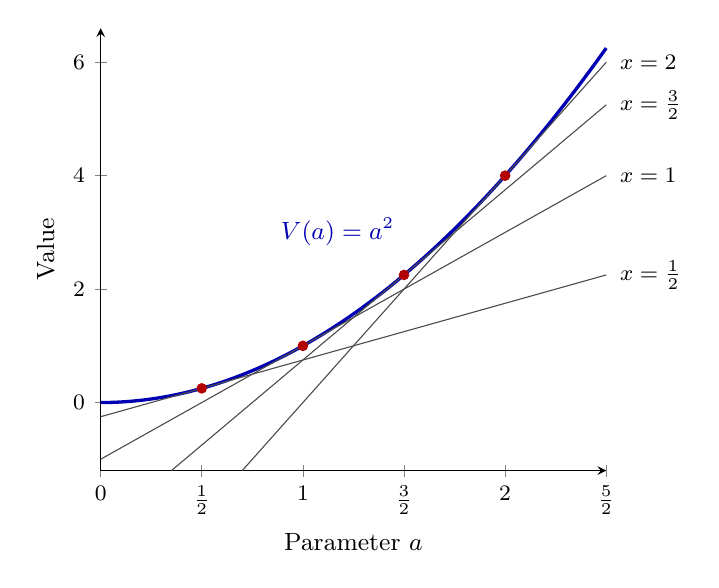
\begin{tikzpicture}
\begin{axis}[
  width=0.66\textwidth, height=7.2cm,
  xmin=0, xmax=2.5, ymin=-1.2, ymax=6.6,
  xlabel={Parameter $a$}, ylabel={Value},
  xtick={0,0.5,1,1.5,2,2.5}, xticklabels={$0$,$\frac{1}{2}$,$1$,$\frac{3}{2}$,$2$,$\frac{5}{2}$},
  tick label style={font=\footnotesize}, label style={font=\small},
  axis lines=left, clip=false]
  \addplot[domain=0:2.5, samples=100, very thick, blue!70!black] {x^2};
  \addplot[domain=0:2.5, samples=2, thin, black!70] {x - 0.25};
  \addplot[domain=0:2.5, samples=2, thin, black!70] {2*x - 1};
  \addplot[domain=0.35:2.5, samples=2, thin, black!70] {3*x - 2.25};
  \addplot[domain=0.7:2.5, samples=2, thin, black!70] {4*x - 4};
  \addplot[only marks, mark=*, mark size=1.7pt, red!70!black] coordinates {(0.5,0.25) (1,1) (1.5,2.25) (2,4)};
  \node[anchor=west, font=\footnotesize] at (axis cs:2.52,2.25) {$x = \frac{1}{2}$};
  \node[anchor=west, font=\footnotesize] at (axis cs:2.52,4) {$x = 1$};
  \node[anchor=west, font=\footnotesize] at (axis cs:2.52,5.25) {$x = \frac{3}{2}$};
  \node[anchor=west, font=\footnotesize] at (axis cs:2.52,6) {$x = 2$};
  \node[anchor=south east, font=\small, blue!70!black] at (axis cs:1.5,2.6) {$V(a) = a^2$};
\end{axis}
\end{tikzpicture}
\caption{The envelope theorem. Each thin line is $f(x, a) = 2xa - x^2$ for a fixed choice $x \in \{\frac{1}{2}, 1, \frac{3}{2}, 2\}$.
The value function $V(a) = \max_x f(x, a) = a^2$, attained at $x^*(a) = a$, is their upper envelope. Each line touches the
envelope at $a = x$ (dots), so $V'(a) = \frac{\partial f}{\partial a}(x^*(a), a) = 2x^*(a) = 2a$. The envelope is convex because
it is a maximum of functions linear in $a$.}
\label{fig:B-envelope}
\end{figure}

\subsection{The envelope theorem with constraints}\label{sec:B-envelope-constrained}

\begin{theorem}[Envelope theorem with constraints]\label{thm:B-envelope-constrained}
In problem \eqref{eq:B-constrained} with scalar $a$, let $f$ and the $g_k$ be $C^1$ in $(x, a)$. Suppose that near $a$
the solution $x^*(a)$ and multipliers $\lambda^*(a)$ are differentiable, satisfy the conditions of \cref{thm:B-kkt}, and
that the set of binding constraints does not change. Then
\begin{equation}\label{eq:B-envelope-constrained}
V'(a) = \frac{\partial \mathcal{L}}{\partial a}\big(x^*(a), \lambda^*(a), a\big)
= f_a\big(x^*(a), a\big) + \sum_{k}\lambda_k^*(a)\,\frac{\partial g_k}{\partial a}\big(x^*(a), a\big) .
\end{equation}
\end{theorem}

\begin{proof}
Write $V(a) = f(x^*(a), a)$ and differentiate:
\begin{equation*}
V'(a) = \nabla_x f^\top\frac{\dd x^*}{\dd a} + f_a .
\end{equation*}
Stationarity replaces $\nabla_x f$ by $-\sum_k\lambda_k^*\nabla_x g_k$:
\begin{equation*}
V'(a) = -\sum_k\lambda_k^*\,\nabla_x g_k^\top\frac{\dd x^*}{\dd a} + f_a .
\end{equation*}
A binding constraint satisfies $g_k(x^*(a), a) = 0$ on a neighborhood of $a$. Differentiating this identity gives
$\nabla_x g_k^\top\frac{\dd x^*}{\dd a} = -\frac{\partial g_k}{\partial a}$. A slack constraint has $\lambda_k^* = 0$ on a
neighborhood. Substituting both facts yields \eqref{eq:B-envelope-constrained}.
\end{proof}

\begin{corollary}[Multipliers as shadow prices]\label{cor:B-shadow}
If a constraint takes the form $h(x) \leq b$, the derivative of the value with respect to $b$ equals its multiplier,
$\frac{\partial V}{\partial b} = \lambda^*$.
\end{corollary}

\begin{proof}
Write the constraint as $g(x, b) = b - h(x) \geq 0$. Then $\frac{\partial g}{\partial b} = 1$, the objective does not depend
on $b$, and \eqref{eq:B-envelope-constrained} gives $V'(b) = \lambda^*$.
\end{proof}

In \cref{ex:B-cobb-douglas}, the budget constraint is $p^\top q \leq I$, and indeed $\frac{\partial v}{\partial I} = \frac{1}{I} = \lambda$.
The multiplier on a budget is the marginal utility of income, and the multiplier on an output constraint in cost
minimization is marginal cost (\cref{ex:B-shephard-cost}).

\begin{remark}[The Le Chatelier principle]\label{rem:B-lechatelier}
Split the choice into $x = (y, z)$, where $z$ is fixed at $\bar z$ in the short run. The long-run value
$V^L(a) = \max_{y, z}f(y, z, a)$ is at least the short-run value $V^S(a) = \max_yf(y, \bar z, a)$, with equality at the
$a_0$ for which $\bar z$ is optimal. The difference $V^L - V^S$ is therefore minimized at $a_0$. Its first derivative
vanishes there and its second derivative is nonnegative, so ${V^L}'(a_0) = {V^S}'(a_0)$ and
${V^L}''(a_0) \geq {V^S}''(a_0)$. When $V'$ is a supply or demand function, as with Hotelling's lemma below, long-run
responses are at least as large as short-run ones \citep{Samuelson1947}. For costs the inequality flips. Long-run cost
is the lower envelope of short-run cost curves and touches the one with the optimal capital stock. At that output,
long-run and short-run marginal cost coincide, and long-run marginal cost is flatter. This is one reason why
accounting measures of cost can differ from the economic marginal cost that pricing theory needs (\cref{ch:intro}).

Rationing gives a concrete case in consumer theory \citep[Section~4.3, pp.~110--112]{DeatonMuellbauer1980b}.
Let good 1 be rationed at the quantity the consumer would choose freely, $z = h_1(p, u)$, where $h$ is
Hicksian demand and $S_{jk} = \frac{\partial h_j}{\partial p_k}$ (\cref{sec:B-shephard}). Write
$h_j^*(p_{-1}, u, z)$ for the restricted Hicksian demand for good $j \neq 1$ (\cref{rem:B-rationing}). It does
not depend on $p_1$, and $h_j^*(p_{-1}, u, h_1(p, u)) = h_j(p, u)$ for all $p$ (their eq.~3.3).
\Cref{sec:05-welfare-virtual} differentiates this identity with respect to $p_1$ and $p_j$ and uses Slutsky
symmetry (\cref{prop:B-slutsky-matrix}). With $S_{11} < 0$, the restricted own-price effect is
\begin{equation*}
S^*_{jj} \equiv \frac{\partial h_j^*}{\partial p_j} = S_{jj} - \frac{S_{j1}^2}{S_{11}} \geq S_{jj},
\end{equation*}
their eq.~3.6 (p.~112). Both sides are nonpositive, so rationing good 1 weakly reduces the absolute
compensated own-price effect of every other good. The reduction is zero only when $S_{j1} = 0$.
\end{remark}

\subsection{Applications}\label{sec:B-envelope-apps}

\begin{example}[Hotelling's lemma]\label{ex:B-hotelling}
A price-taking firm with production function $\varphi(x)$, output price $p$ and input prices $r$ earns
\begin{equation*}
\pi(p, r) = \max_x\ p\,\varphi(x) - r^\top x .
\end{equation*}
\Cref{thm:B-envelope} gives
\begin{equation*}
\frac{\partial \pi}{\partial p} = \varphi(x^*) = q^* , \qquad \frac{\partial \pi}{\partial r_\ell} = -x_\ell^* ,
\end{equation*}
so supply and input demands are derivatives of the profit function \citep{Hotelling1932}. For each $x$, the objective is
linear in $(p, r)$. By \cref{lem:B-minlinear}, $\pi$ is convex in $(p, r)$. Its second derivatives therefore give
$\frac{\partial q^*}{\partial p} = \frac{\partial^2 \pi}{\partial p^2} \geq 0$ and $\frac{\partial x_\ell^*}{\partial r_\ell} = -\frac{\partial^2 \pi}{\partial r_\ell^2} \leq 0$:
supply curves slope up and input demand curves slope down.
\end{example}

\begin{example}[Shephard's lemma and marginal cost]\label{ex:B-shephard-cost}
The cost function is $C(r, q) = \min_x\{r^\top x : \varphi(x) \geq q\}$. Write it as the maximization problem
$-C(r, q) = \max_x\{-r^\top x : \varphi(x) - q \geq 0\}$, with Lagrangian $-r^\top x + \lambda(\varphi(x) - q)$.
\Cref{thm:B-envelope-constrained} gives
\begin{equation*}
\frac{\partial C}{\partial r_\ell} = x_\ell(r, q) , \qquad \frac{\partial C}{\partial q} = \lambda^* ,
\end{equation*}
the first being Shephard's lemma for costs \citep{Shephard1953}. The multiplier on the output constraint is marginal
cost. Stationarity reads $r_\ell = \lambda^*\frac{\partial \varphi}{\partial x_\ell}$, so each input price equals marginal cost times
the input's marginal product. Multiplying by $\frac{x_\ell}{q}$ for a freely adjustable input $\ell$ and dividing the output
price $p$ by $\lambda^*$,
\begin{equation*}
\frac{p}{\lambda^*} = \Big(\frac{\partial \varphi}{\partial x_\ell}\frac{x_\ell}{q}\Big)\frac{pq}{r_\ell x_\ell} .
\end{equation*}
The markup ratio equals the output elasticity of the flexible input times the ratio of revenue to spending on that
input. This is the production approach to markups (\cref{prop:01-production-markup}, \citealp{DeLoeckerWarzynski2012}).
Concavity of $C$ in $r$ follows from \cref{lem:B-minlinear}.
\end{example}

\begin{example}[Monopoly profit, cost and taxes]\label{ex:B-monopoly-tax}
A monopolist with constant marginal cost $c$ and specific tax $t$ earns $\pi^*(t) = \max_p(p - c - t)Q(p)$. The envelope
theorem gives $\frac{\dd \pi^*}{\dd t} = -Q(p^*)$. To first order, profit falls by the quantity sold whatever the
pass-through rate. Consumer surplus $\int_{p^*}^{\infty}Q(u)\,\dd u$ falls at rate $Q\frac{\dd p^*}{\dd t} = \rho Q$ by Leibniz's
rule. The ratio of consumer to producer burden under monopoly is therefore $\rho$, the case $\theta = 1$ of
\cref{prop:02-incidence}.
\end{example}

\begin{example}[Entry lowers incumbents' Cournot profits]\label{ex:B-cournot-entry}
Firm $i$'s profit given rivals' output is $V_i(Q_{-i}) = \max_{q_i}\big[P(q_i + Q_{-i})q_i - C_i(q_i)\big]$. By the envelope
theorem,
\begin{equation*}
V_i'(Q_{-i}) = q_i\,P'(Q) < 0 \qquad\text{whenever } q_i > 0 .
\end{equation*}
The firm's own output response has no first-order effect. In a symmetric equilibrium with $N$ firms, rivals' output is
$Q_{-i} = Q - q$, and entry raises it, since $\frac{\dd Q}{\dd N} > 0$ and $\frac{\dd q}{\dd N} < 0$ (\cref{prop:02-entry-cs}).
Treating $N$ as continuous,
\begin{equation*}
\frac{\dd \pi}{\dd N} = q\,P'(Q)\Big(\frac{\dd Q}{\dd N} - \frac{\dd q}{\dd N}\Big) < 0 .
\end{equation*}
\end{example}

\begin{example}[Bidder rents in the first-price auction]\label{ex:B-auction-envelope}
There are $n$ bidders with independent private values drawn from $F$, and a reserve price $r$. Rivals use a strictly
increasing bid function $\beta$ with $\beta(r) = r$. A bidder with value $v \geq r$ who bids $\beta(z)$ wins when every rival
value is below $z$, with probability $F(z)^{n - 1}$. Her equilibrium payoff is
\begin{equation*}
\pi(v) = \max_{z}\ \big(v - \beta(z)\big)F(z)^{n - 1} ,
\end{equation*}
and in equilibrium $z = v$ is optimal. For each $z$ the objective is affine in $v$ with slope $F(z)^{n - 1}$. So $\pi$ is a
maximum of affine functions, hence convex and absolutely continuous, and \cref{thm:B-envelope-integral} applies:
\begin{equation*}
\pi'(v) = F(v)^{n - 1} \ \text{almost everywhere}, \qquad \pi(r) = \big(r - \beta(r)\big)F(r)^{n - 1} = 0 .
\end{equation*}
Integrating from $r$ gives $\pi(v) = \int_r^vF(t)^{n - 1}\,\dd t$. The payoff is also the winning probability times the
surplus when winning, $\pi(v) = (v - \beta(v))F(v)^{n - 1}$. Equating the two expressions,
\begin{equation*}
\beta(v) = v - \frac{\int_r^vF(t)^{n - 1}\,\dd t}{F(v)^{n - 1}} ,
\end{equation*}
which is \eqref{eq:B-rs-bid}. With uniform values on $[0, 1]$ and $r = 0$, $\beta(v) = \frac{n - 1}{n}v$.

The first-order route reaches the same formula with more work. Differentiating the objective in $z$ at $z = v$ gives
$-\beta'(v)F(v)^{n - 1} + (v - \beta(v))(n - 1)F(v)^{n - 2}f(v) = 0$. Rearranged, this is the differential equation
\begin{equation*}
\frac{\dd}{\dd v}\Big[\beta(v)F(v)^{n - 1}\Big] = v\,\frac{\dd}{\dd v}\Big[F(v)^{n - 1}\Big] .
\end{equation*}
Integrating from $r$ and applying the integration by parts of \cref{ex:B-rs-parts} gives the bid again. The envelope
route needs neither the differential equation nor differentiability of $\beta$. It also shows that the payoff
$\pi(v)$ depends only on who wins and on the zero payoff of type $r$. Any format with the same allocation and
$\pi(r) = 0$ therefore yields the same expected payments, which is revenue equivalence \citep{Myerson1981,
RileySamuelson1981}. \Cref{sec:14-fpa-envelope} develops these results.
\end{example}

\begin{example}[Expected maximum utility]\label{ex:B-logsum-envelope}
Let $\mathcal{W}(\delta) = \E[\max_k(\delta_k + \epsilon_k)]$ in an additive random utility model with continuously distributed
errors. For each realization of $\epsilon$, the maximum is the value of a choice over a finite set. Its derivative in
$\delta_j$ is $\indic\{j \text{ is the maximizer}\}$ wherever the maximizer is unique, which holds with probability one.
This is the envelope theorem for a finite choice set. Taking expectations,
\begin{equation*}
\frac{\partial \mathcal{W}}{\partial \delta_j} = \Pr(j \text{ is chosen}) = s_j(\delta) .
\end{equation*}
The exchange of derivative and expectation needs a domination argument, which the Williams-Daly-Zachary theorem
(\cref{thm:B-wdz}) supplies. In the logit, $\mathcal{W} = \ln\sum_ke^{\delta_k}$ plus a constant, and
$\frac{\partial}{\partial \delta_j}\ln\sum_ke^{\delta_k} = s_j$.
\end{example}

\section{Duality in consumer and producer theory}\label{sec:B-duality}

Duality theory studies an optimization problem through its value function. Under convexity the value
function summarizes the problem completely, and its derivatives deliver the demand or supply functions. The
envelope theorem of \cref{sec:B-envelope} computes those derivatives, so this section applies it repeatedly.
Empirical IO uses this in three ways. It builds demand systems from an expenditure function, as in the
almost ideal demand system of \cref{ch:aids}. It measures welfare exactly from estimated demand, as in the
valuation of new goods in \cref{ch:newgoods}. It recovers marginal cost from a cost function, as in the
conduct and airline studies of \cref{ch:conduct} and \cref{ch:airlines}. \Cref{sec:05-duality} proves the
consumer-theory results that the AIDS needs. This section restates them for reference and points to those
proofs. It adds five tools: the envelope-theorem proof of Shephard's lemma, the properties of indirect
utility, the integrability method of \citet{Hausman1981}, quasi-linear utility and producer duality.

There are $n$ goods indexed by $i, j = 1, \dots, n$, with prices $p \in \R^n_{++}$. In this section $I > 0$
denotes the consumer's income (total expenditure), not the number of consumers. We write $U$ for the
utility function and $u$ for a utility level. Marshallian demand is $q(p, I)$ and Hicksian demand is
$h(p, u)$. The indirect utility function is $v(p, I)$ and the expenditure function is $e(p, u)$. The budget
share of good $i$ is $w_i = \frac{p_iq_i}{I}$, the income elasticity is
$\eta_i = \frac{\partial\ln q_i}{\partial\ln I}$, and the Slutsky matrix $S$ has elements
$S_{ij} = \frac{\partial h_i}{\partial p_j}$. In this section only, $\varepsilon_{ij}$ denotes the signed
Marshallian elasticity $\frac{\partial\ln q_i}{\partial\ln p_j}$, as in \cref{ch:aids}.

\subsection{The utility maximization and expenditure minimization problems}\label{sec:B-ump-emp}

\begin{assumption}[Preferences]\label{ass:B-preferences}
The utility function $U : \R^n_+ \to \R$ is continuous, strictly increasing and strictly quasi-concave.
Prices satisfy $p \gg 0$, meaning that every component is positive, and income satisfies $I > 0$.
\end{assumption}

The \emph{utility maximization problem} (UMP) and the \emph{expenditure minimization problem} (EMP) are
\begin{equation}\label{eq:B-ump-emp}
v(p, I) = \max_{q \geq 0}\big\{U(q) : p^\T q \leq I\big\},
\qquad
e(p, u) = \min_{q \geq 0}\big\{p^\T q : U(q) \geq u\big\}.
\end{equation}
The maximizer $q(p, I)$ is the \emph{Marshallian demand}, and the minimizer $h(p, u)$ is the
\emph{Hicksian} (compensated) \emph{demand}. In the EMP we take utility levels $u > U(0)$ in the range of
$U$. Both problems have solutions. The budget set is compact because $p \gg 0$, and a continuous function
attains its maximum on a compact set. For the EMP, pick any bundle $\bar q$ with $U(\bar q) \geq u$ and
minimize over the compact set $\{q \geq 0 : U(q) \geq u,\ p^\T q \leq p^\T\bar q\}$. The solutions are
unique. If two distinct bundles solved the UMP, their midpoint would be affordable and, by strict
quasi-concavity, strictly better. The argument for the EMP is the same after scaling the midpoint down
slightly. Both constraints bind. A bundle that leaves money unspent can be enlarged, which raises utility
because $U$ is strictly increasing.

\begin{proposition}[Indirect utility function]\label{prop:B-v-properties}
Under \cref{ass:B-preferences}, $v(p, I)$ has four properties.
\begin{enumerate}[label=(\roman*)]
\item It is homogeneous of degree zero in $(p, I)$.
\item It is strictly increasing in $I$ and nonincreasing in each $p_i$.
\item It is quasi-convex in $p$: for every $\bar v$, the set $\{p : v(p, I) \leq \bar v\}$ is convex.
\item It is continuous in $(p, I)$.
\end{enumerate}
\end{proposition}

\begin{proof}
Write $B(p, I) = \{q \geq 0 : p^\T q \leq I\}$ for the budget set. (i) For $\lambda > 0$,
$B(\lambda p, \lambda I) = B(p, I)$, so the two maxima coincide. (ii) If $I' > I$, the bundle $q(p, I)$
costs $I < I'$, so $q(p, I) + \epsilon\mathbf{1}$ is affordable at $I'$ for small $\epsilon > 0$ and is
strictly better. If $p' \geq p$, then $B(p', I) \subseteq B(p, I)$, so $v(p', I) \leq v(p, I)$. (iii) Let
$p'' = \lambda p + (1 - \lambda)p'$ with $\lambda \in [0, 1]$. Any $q$ with $p''^\T q \leq I$ satisfies
$p^\T q \leq I$ or $p'^\T q \leq I$, because otherwise $p''^\T q > I$. Hence
$B(p'', I) \subseteq B(p, I) \cup B(p', I)$ and
\begin{equation*}
v(p'', I) \leq \max\{v(p, I), v(p', I)\}.
\end{equation*}
If both $v(p, I)$ and $v(p', I)$ are at most $\bar v$, so is $v(p'', I)$. (iv) The objective is continuous
and the budget correspondence is continuous and compact-valued when $p \gg 0$, so the theorem of the
maximum applies \citep[ch.~3]{MasColellWhinstonGreen1995}.
\end{proof}

\begin{proposition}[Expenditure function]\label{prop:B-e-properties}
Under \cref{ass:B-preferences}, $e(p, u)$ has four properties.
\begin{enumerate}[label=(\roman*)]
\item It is homogeneous of degree one in $p$.
\item It is strictly increasing in $u$ and nondecreasing in each $p_i$.
\item It is concave in $p$.
\item It is continuous in $(p, u)$.
\end{enumerate}
\end{proposition}

\Cref{prop:05-e-properties} proves the four properties. Concavity is the key one. For each feasible bundle
$q$ the map $p \mapsto p^\T q$ is linear, and $e(\cdot, u)$ is the minimum of this family, which is concave by
\cref{lem:B-minlinear}.

\begin{proposition}[Duality identities]\label{prop:B-duality-identities}
Under \cref{ass:B-preferences}, for all $p \gg 0$, $I > 0$ and $u > U(0)$ in the range of $U$,
\begin{align}
e(p, v(p, I)) &= I, & v(p, e(p, u)) &= u, \label{eq:B-duality-1}\\
q(p, I) &= h(p, v(p, I)), & h(p, u) &= q(p, e(p, u)). \label{eq:B-duality-2}
\end{align}
\end{proposition}

\Cref{lem:05-duality} proves the identities. The argument uses monotonicity and continuity of $U$ to show that
each constraint binds, and uniqueness of the solutions to match the two demands.

The identities let us move between the two problems. The functions $v(p, \cdot)$ and $e(p, \cdot)$ are
inverses of each other for fixed prices, and Marshallian and Hicksian demands coincide when income and
utility are linked by them. Every result below uses one of the four identities.

\citet[ch.~2]{DeatonMuellbauer1980b} build demand analysis on the same duality. They write the expenditure
function as the \emph{cost function} $c(u, p)$ and income as total outlay $x$. Their Section~2.3
(pp.~37--42) states the properties of \cref{prop:B-e-properties} and derives Shephard's lemma and Roy's
identity (their eqs.~3.9 and 3.16, pp.~40--41). Section~2.4 (pp.~43--46) derives adding up, homogeneity,
symmetry, negativity and the Slutsky equation (eqs.~4.1--4.6). Section~2.5 (pp.~47--50) turns to the
integrability problem of \cref{sec:B-integrability}.

\subsection{Shephard's lemma, Roy's identity and the Slutsky equation}\label{sec:B-shephard}

\begin{proposition}[Shephard's lemma, \citealp{Shephard1953}]\label{prop:B-shephard}
Under \cref{ass:B-preferences}, if $e(\cdot, u)$ is differentiable at $p^0$, then
\begin{equation}\label{eq:B-shephard}
h_i(p^0, u) = \frac{\partial e(p^0, u)}{\partial p_i}, \qquad i = 1, \dots, n .
\end{equation}
In share form, at $u = v(p, I)$,
\begin{equation}\label{eq:B-shephard-share}
w_i = \frac{\partial\ln e(p, u)}{\partial\ln p_i} .
\end{equation}
\end{proposition}

\Cref{prop:05-shephard} proves the lemma with a supporting-hyperplane argument and derives the share form by
the chain rule. Here we give the second route, through the envelope theorem.

\begin{proof}[Proof (envelope theorem)]
Suppose $U$ is twice continuously differentiable and the solution $(h(p, u), \mu(p, u))$ of the EMP and
its multiplier are differentiable in $p$. The Lagrangian is
$\mathcal{L}(q, \mu, p) = p^\T q - \mu\,[U(q) - u]$. The envelope theorem with constraints
(\cref{thm:B-envelope-constrained}) says that the derivative of the value function equals the partial
derivative of the Lagrangian, evaluated at the solution:
\begin{equation*}
\frac{\partial e(p, u)}{\partial p_i} = \frac{\partial\mathcal{L}}{\partial p_i}\Big|_{q = h(p, u),\,\mu = \mu(p, u)}
= h_i(p, u).
\end{equation*}
The indirect effects through $q$ and $\mu$ vanish by the first-order conditions and the binding
constraint. The share form follows by the chain rule, as in \cref{sec:05-shephard}.
\end{proof}

The supporting-hyperplane proof of \cref{prop:05-shephard} needs neither derivatives of $U$ nor
differentiability of $h$. Fix $p^0$ and let $q^0 = h(p^0, u)$. The bundle $q^0$ is feasible at every price
vector, so $e(p, u) \leq p^\T q^0$, with equality at $p^0$. The gradient of $p^\T q^0 - e(p, u)$ therefore
vanishes at its minimizer $p^0$. This is the proof of \citet[eqs.~3.10--3.11, p.~40]{DeatonMuellbauer1980b},
whose function $Z(p)$ is $p^\T q^0 - e(p, u)$. It also shows more. The same argument works for any bundle $q$ in
the Hicksian demand set. So every such bundle is a \emph{supergradient}
of the concave function $e(\cdot, u)$ at $p^0$, that is, $e(p, u) \leq e(p^0, u) + q^\T(p - p^0)$ for every $p$. When indifference curves have flat segments, the Hicksian
demand is a set and $e$ has a kink. \Cref{fig:B-expfn} draws the argument. Figure~2.9 of
\citet[p.~39]{DeatonMuellbauer1980b} draws the same concave cross section, with a chord in place of the
supporting lines. \citet{DeatonMuellbauer1980a}
state the share form \eqref{eq:B-shephard-share} as their equation (5) on p.~313, with the cost function
written $c(u, p)$. Logarithmic differentiation of an expenditure function then yields budget shares as
functions of prices and utility, which is how they derive the AIDS.

\begin{figure}[htbp]
\centering
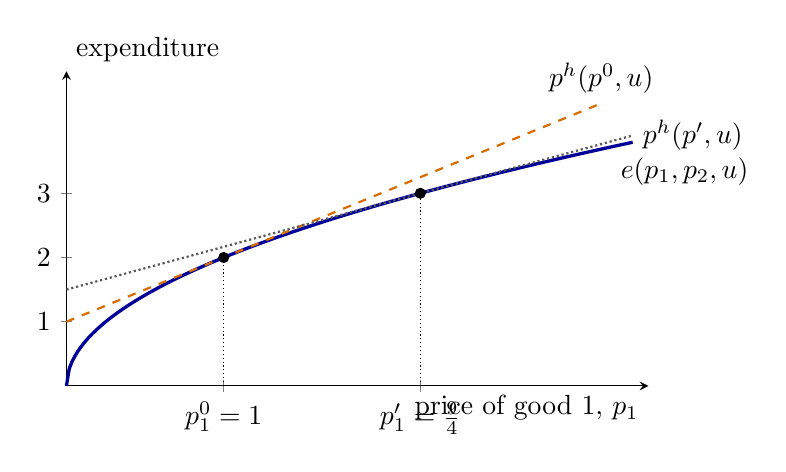
\begin{tikzpicture}
\begin{axis}[
  width=0.74\textwidth, height=0.46\textwidth,
  axis lines=left, xmin=0, xmax=3.7, ymin=0, ymax=4.9,
  xlabel={price of good 1, $p_1$}, ylabel={expenditure},
  xtick={1,2.25}, xticklabels={$p_1^0 = 1$,$p_1' = \frac{9}{4}$},
  ytick={1,2,3}, yticklabels={$1$,$2$,$3$},
  every axis x label/.style={at={(ticklabel* cs:1)}, anchor=north east},
  every axis y label/.style={at={(ticklabel* cs:1)}, anchor=south west},
  clip=false]
\addplot[domain=0:3.6, samples=200, very thick, blue!60!black] {2*sqrt(x)}
  node[pos=0.97, below right, black] {$e(p_1, p_2, u)$};
\addplot[domain=0:3.4, thick, dashed, orange!85!black] {x + 1}
  node[pos=1, above, black] {$p^\T h(p^0, u)$};
\addplot[domain=0:3.6, thick, densely dotted, gray!70!black] {(2/3)*x + 1.5}
  node[pos=1, right, black] {$p^\T h(p', u)$};
\addplot[only marks, mark=*, mark size=1.8pt] coordinates {(1,2) (2.25,3)};
\draw[densely dotted] (axis cs:1,0) -- (axis cs:1,2);
\draw[densely dotted] (axis cs:2.25,0) -- (axis cs:2.25,3);
\end{axis}
\end{tikzpicture}
\caption{Shephard's lemma as a supporting hyperplane. Cobb-Douglas utility
$U = q_1^{\frac{1}{2}}q_2^{\frac{1}{2}}$ with $p_2 = 1$ and $u = 1$ gives $e(p_1, 1, 1) = 2\sqrt{p_1}$, which is
concave in $p_1$. The cost of the fixed bundle $h(p^0, u) = (1, 1)$ is the line $p_1 + 1$. It lies above
$e$ and touches it at $p_1^0 = 1$, so its slope $h_1(p^0, u) = 1$ equals the slope of $e$ there. The dotted
line repeats the construction at $p_1' = \frac{9}{4}$, where $h(p', u) = (\frac{2}{3}, \frac{3}{2})$. The
expenditure function is the lower envelope of all such lines.}\label{fig:B-expfn}
\end{figure}

\begin{proposition}[Roy's identity, \citealp{Roy1947}]\label{prop:B-roy}
Under \cref{ass:B-preferences}, if $v$ is differentiable at $(p, I)$ with $\frac{\partial v}{\partial I} > 0$
and $e(\cdot, u)$ is differentiable at $p$ for $u = v(p, I)$, then
\begin{equation}\label{eq:B-roy}
q_i(p, I) = -\frac{\partial v(p, I)}{\partial p_i}\left[\frac{\partial v(p, I)}{\partial I}\right]^{-1}.
\end{equation}
\end{proposition}

\Cref{prop:05-roy} proves the identity, together with its share form. The proof differentiates the identity
$v(p, e(p, u)) = u$ of \eqref{eq:B-duality-1} with respect to $p_i$, substitutes Shephard's lemma, and
evaluates at $u = v(p, I)$.

Roy's identity is invariant to increasing transformations of $v$, because a transformation multiplies both
derivatives by the same positive factor. \Cref{sec:B-logsum} shows that the Williams-Daly-Zachary theorem is
the discrete-choice version of the identity.

\begin{proposition}[Slutsky equation, \citealp{Slutsky1915}]\label{prop:B-slutsky}
Under \cref{ass:B-preferences} and differentiability of $q$ and $h$, at $u = v(p, I)$,
\begin{equation}\label{eq:B-slutsky}
\frac{\partial q_i(p, I)}{\partial p_j} = \frac{\partial h_i(p, u)}{\partial p_j} - q_j(p, I)\,\frac{\partial q_i(p, I)}{\partial I} .
\end{equation}
In elasticity form, $\varepsilon^h_{ij} = \varepsilon_{ij} + \eta_iw_j$, where
$\varepsilon^h_{ij} = \frac{\partial\ln h_i}{\partial\ln p_j}$ is the Hicksian elasticity.
\end{proposition}

\Cref{prop:05-slutsky}(i) proves the equation by differentiating $h_i(p, u) = q_i(p, e(p, u))$ with respect to
$p_j$ and applying Shephard's lemma. \Cref{prop:05-elast-identities}(a) derives the elasticity form.

The first term on the right of \eqref{eq:B-slutsky} is the \emph{substitution effect}, which holds utility
fixed. The second is the \emph{income effect}, the response to the loss of purchasing power. The remaining
elasticity identities (Engel and Cournot aggregation, homogeneity, symmetry in share form) are derived in
\cref{sec:05-elasticity-identities}.

\begin{proposition}[Slutsky matrix]\label{prop:B-slutsky-matrix}
Suppose $e(\cdot, u)$ is twice continuously differentiable. Then the Slutsky matrix $S(p, u)$ satisfies:
\begin{enumerate}[label=(\roman*)]
\item $S$ is symmetric: $S_{ij} = S_{ji}$.
\item $S$ is negative semidefinite. In particular $S_{ii} \leq 0$.
\item $Sp = 0$ and $p^\T S = 0$. Hence $S$ has rank at most $n - 1$.
\end{enumerate}
\end{proposition}

\begin{proof}
By Shephard's lemma, $S$ is the Hessian of $e(\cdot, u)$. Parts (ii) to (iv) of \cref{prop:05-slutsky} prove
symmetry, negative semidefiniteness and $Sp = 0$ from Young's theorem, concavity and Euler's theorem
(\cref{prop:B-euler}). Symmetry then gives $p^\T S = 0$. The vector $p$ is nonzero and lies in the null space,
so the rank of $S$ is at most $n - 1$.
\end{proof}

\begin{corollary}[Net substitutes]\label{cor:B-net-substitutes}
If $n \geq 2$ and $S_{ii} < 0$, then $S_{ij} > 0$ for at least one $j \neq i$. Every good with a strictly
negative compensated own-price effect has at least one net substitute.
\end{corollary}

\begin{proof}
Row $i$ of $Sp = 0$ reads $\sum_{j \neq i}S_{ij}p_j = -S_{ii}p_i > 0$. Since every $p_j > 0$, at least one
$S_{ij}$ with $j \neq i$ must be positive.
\end{proof}

Negative semidefiniteness is the compensated law of demand. It is the only sign restriction that consumer
theory places on demand. Marshallian own-price effects can have either sign, because the income effect in
\eqref{eq:B-slutsky} can dominate.

\begin{example}[Cobb-Douglas duality, continuing \cref{ex:B-cobb-douglas}]\label{ex:B-cd-duality}
Let $U(q) = \prod_iq_i^{a_i}$ with $a_i > 0$ and $\sum_ia_i = 1$. This is an increasing transformation of
$\sum_ia_i\ln q_i$, so Marshallian demand is again $q_i = \frac{a_iI}{p_i}$. Substituting demand into $U$,
\begin{equation*}
v(p, I) = \prod_i\left(\frac{a_iI}{p_i}\right)^{a_i} = I\prod_i\left(\frac{a_i}{p_i}\right)^{a_i}.
\end{equation*}
Setting $v(p, e) = u$ and solving for $e$ gives the expenditure function
\begin{equation*}
e(p, u) = u\prod_i\left(\frac{p_i}{a_i}\right)^{a_i}.
\end{equation*}
It is homogeneous of degree one in $p$ because the exponents sum to one. Shephard's lemma gives
$h_i(p, u) = \frac{\partial e}{\partial p_i} = \frac{a_i}{p_i}e(p, u)$. At $u = v(p, I)$ we have $e = I$, so
$h_i = \frac{a_iI}{p_i} = q_i$, as \eqref{eq:B-duality-2} requires. Roy's identity also recovers demand:
\begin{equation*}
\frac{\partial v}{\partial p_i} = -\frac{a_i}{p_i}v, \qquad \frac{\partial v}{\partial I} = \frac{v}{I},
\qquad -\frac{\partial v}{\partial p_i}\left[\frac{\partial v}{\partial I}\right]^{-1} = \frac{a_iI}{p_i}.
\end{equation*}
For the Slutsky equation with $i \neq j$, the compensated cross effect is
$S_{ij} = \frac{a_i}{p_i}\frac{\partial e}{\partial p_j} = \frac{a_ia_je}{p_ip_j}$, which is symmetric in
$(i, j)$. The Marshallian cross effect is zero, and the income term is
$q_j\frac{\partial q_i}{\partial I} = \frac{a_jI}{p_j}\cdot\frac{a_i}{p_i}$. At $e = I$ the two sides of
\eqref{eq:B-slutsky} agree. The own effect is
$S_{ii} = \frac{a_i}{p_i}\cdot\frac{a_ie}{p_i} - \frac{a_ie}{p_i^2} = -\frac{a_i(1 - a_i)e}{p_i^2} < 0$, and
row $i$ of $Sp$ is $\frac{a_ie}{p_i}\left(\sum_ja_j - 1\right) = 0$.
\end{example}

\begin{example}[PIGLOG preferences, \citealp{DeatonMuellbauer1980a}]\label{ex:B-piglog}
The \emph{PIGLOG} (price-independent generalized logarithmic) class of
\citet[eq.~1, p.~313]{DeatonMuellbauer1980a} has
\begin{equation*}
\ln e(p, u) = (1 - u)\ln a(p) + u\ln b(p).
\end{equation*}
Here $a(p)$ and $b(p)$ are positive and homogeneous of degree one. They are interpreted as the costs of
subsistence ($u = 0$) and bliss ($u = 1$). The share form of Shephard's lemma gives
\begin{equation*}
w_i = \frac{\partial\ln a}{\partial\ln p_i} + u\left(\frac{\partial\ln b}{\partial\ln p_i} - \frac{\partial\ln a}{\partial\ln p_i}\right).
\end{equation*}
Inverting $\ln e(p, u) = \ln I$ gives the indirect utility function
$u = \frac{\ln I - \ln a(p)}{\ln b(p) - \ln a(p)}$. Substituting it into the share equation shows that budget
shares are linear in $\ln I$, with coefficients that depend on prices. The AIDS chooses a translog
$\ln a(p)$ and $\ln b(p) = \ln a(p) + \beta_0\prod_kp_k^{\beta_k}$ \citep[eqs.~2--4]{DeatonMuellbauer1980a}.
\Cref{sec:05-aids} carries out that specialization.
\end{example}

\subsection{Integrability and recovering preferences from demand}\label{sec:B-integrability}

Demand is usually estimated before anything is known about preferences. Two questions follow. Is the
estimated system generated by some utility function? If so, can we recover the expenditure function from
it, so that welfare can be measured exactly? The first question is answered by the integrability theorem.
The second is answered by a differential equation.

\begin{proposition}[Integrability, \citealp{HurwiczUzawa1971}]\label{prop:B-integrability}
Let $q(p, I)$ be continuously differentiable on $\R^n_{++} \times \R_{++}$. Suppose it satisfies adding up,
$p^\T q(p, I) = I$, and homogeneity of degree zero in $(p, I)$. Suppose also that the matrix with elements
$S_{ij} = \frac{\partial q_i}{\partial p_j} + q_j\frac{\partial q_i}{\partial I}$ is symmetric and negative
semidefinite at every $(p, I)$. Then, under regularity conditions, there is an increasing and
quasi-concave utility function whose Marshallian demand is $q$.
\end{proposition}

We omit the proof. Its logic is short. We look for a function $e(p, u)$ that satisfies the
system of partial differential equations
\begin{equation}\label{eq:B-integrability-pde}
\frac{\partial e(p, u)}{\partial p_i} = q_i\big(p, e(p, u)\big), \qquad i = 1, \dots, n,
\end{equation}
which combines Shephard's lemma with \eqref{eq:B-duality-2}. Differentiate the $i$-th equation with respect
to $p_j$:
\begin{equation*}
\frac{\partial^2e}{\partial p_j\partial p_i} = \frac{\partial q_i}{\partial p_j} + \frac{\partial q_i}{\partial I}\cdot\frac{\partial e}{\partial p_j}
= \frac{\partial q_i}{\partial p_j} + \frac{\partial q_i}{\partial I}\,q_j = S_{ij}.
\end{equation*}
Mixed partial derivatives must be equal, so a solution can exist only if $S_{ij} = S_{ji}$. This is the
integrability condition of \citet[eqs.~5.2--5.3, p.~50]{DeatonMuellbauer1980b}. Frobenius's
theorem says that symmetry is also sufficient for a local solution. Negative semidefiniteness then makes
the solution concave in $p$, so it is a valid expenditure function
\citep[ch.~3]{MasColellWhinstonGreen1995}. The practical message is that an estimated demand system which
satisfies the four restrictions supports exact welfare analysis (\cref{ch:aids}).

When only one price changes, \eqref{eq:B-integrability-pde} reduces to an ordinary differential equation.
This is the method of \citet{Hausman1981}. Fix the other prices $p_{-1}$ and, for each utility level $u$,
let $\tilde e_u(p_1) = e(p_1, p_{-1}, u)$. Shephard's lemma and \eqref{eq:B-duality-2} give
\begin{equation}\label{eq:B-hausman-ode}
\frac{\dd\tilde e_u(p_1)}{\dd p_1} = h_1(p_1, p_{-1}, u) = q_1\big(p_1, p_{-1}, \tilde e_u(p_1)\big).
\end{equation}
The right side is known once $q_1$ has been estimated, so \eqref{eq:B-hausman-ode} is a first-order
differential equation in the scalar $\tilde e_u$. Each solution curve is one indifference level. We label
the curve by its initial condition. The curve through $(p_1^0, I^0)$ belongs to the utility level
$u^0 = v(p_1^0, p_{-1}, I^0)$, so $\tilde e_{u^0}(p_1^0) = I^0$. If $q_1$ is Lipschitz in income, that is,
$|q_1(p, I) - q_1(p, I')| \leq K|I - I'|$ for a constant $K$, the Picard-Lindel\"of theorem gives a unique solution. Its standard proof is a contraction argument
(\cref{thm:B-banach}). The labeling of utility is arbitrary because utility is ordinal. Money measures such as
the compensating variation do not depend on it.

\citet{Hausman1981} solves \eqref{eq:B-hausman-ode} in closed form for common parametric demands.
\citet[eq.~3, p.~212]{Hausman1997} uses the solution as the ``(partial) expenditure function'' that values a
new cereal brand. The word partial reflects that only the new good's price varies. Under the usual
separability assumptions only the demand curve of the new good needs to be estimated \citep[fn.~7]{Hausman1997}.

\begin{example}[Exact welfare from linear demand]\label{ex:B-hausman-linear}
Let the demand for good 1 be linear in its own price and income,
\begin{equation*}
q_1 = c_0 + c_1p_1 + c_2I, \qquad c_1 < 0,\ c_2 \neq 0,
\end{equation*}
with the other prices fixed and absorbed in $c_0$. Equation \eqref{eq:B-hausman-ode} becomes the linear
equation
\begin{equation*}
\frac{\dd e}{\dd p_1} = c_0 + c_1p_1 + c_2e .
\end{equation*}
\textit{Homogeneous part.} The equation $\frac{\dd e}{\dd p_1} = c_2e$ has the solutions $Ke^{c_2p_1}$ for any
constant $K$.

\textit{Particular solution.} Try $e = A + Bp_1$. Substituting gives $B = c_0 + c_1p_1 + c_2A + c_2Bp_1$ for
all $p_1$. Matching the coefficients on $p_1$ gives $0 = c_1 + c_2B$, so $B = -\frac{c_1}{c_2}$. Matching the
constants gives $B = c_0 + c_2A$, so
\begin{equation*}
A = \frac{B - c_0}{c_2} = -\frac{1}{c_2}\left(c_0 + \frac{c_1}{c_2}\right).
\end{equation*}

\textit{General solution.} Adding the two parts and using the constant of integration as the utility index,
\begin{equation}\label{eq:B-hausman-e}
e(p_1, u) = u\,e^{c_2p_1} - \frac{1}{c_2}\left(c_0 + c_1p_1 + \frac{c_1}{c_2}\right).
\end{equation}
To verify, differentiate: $\frac{\partial e}{\partial p_1} = c_2u\,e^{c_2p_1} - \frac{c_1}{c_2}$. The right
side of the differential equation is
$c_0 + c_1p_1 + c_2u\,e^{c_2p_1} - \left(c_0 + c_1p_1 + \frac{c_1}{c_2}\right)$, which is the same. Inverting
$e(p_1, u) = I$ gives the indirect utility function
\begin{equation*}
v(p_1, I) = e^{-c_2p_1}\left[I + \frac{1}{c_2}\left(c_0 + c_1p_1 + \frac{c_1}{c_2}\right)\right],
\end{equation*}
and Roy's identity returns $q_1$. The Hicksian demand is
$h_1(p_1, u) = c_2u\,e^{c_2p_1} - \frac{c_1}{c_2}$.

\textit{Compensating variation of a price change.} Let the price rise from $p_1^0$ to $p_1^0 + \Delta$ at income
$I^0$, and write $q^0 = c_0 + c_1p_1^0 + c_2I^0$ for initial demand. The initial utility satisfies
$u^0e^{c_2p_1^0} = I^0 + \frac{1}{c_2}\left(c_0 + c_1p_1^0 + \frac{c_1}{c_2}\right) = \frac{q^0}{c_2} + \frac{c_1}{c_2^2}$.
Substituting into $CV = e(p_1^0 + \Delta, u^0) - I^0$ and collecting terms,
\begin{equation}\label{eq:B-hausman-cv}
CV = \left(\frac{q^0}{c_2} + \frac{c_1}{c_2^2}\right)\left(e^{c_2\Delta} - 1\right) - \frac{c_1}{c_2}\Delta .
\end{equation}
Expanding $e^{c_2\Delta}$ to third order shows that $CV \to q^0\Delta + \frac{c_1}{2}\Delta^2$ as $c_2 \to 0$. The
limit is the Marshallian surplus loss $\int_{p_1^0}^{p_1^0 + \Delta}(c_0 + c_1t + c_2I^0)\,\dd t$. Without income
effects the two measures coincide.

\textit{Virtual price and the value of the good.} The virtual price $p_1^V$ is the price at which compensated
demand falls to zero (\cref{def:B-virtual}). The Hicksian slope at the initial point is
$\frac{\partial h_1}{\partial p_1} = c_1 + c_2q^0$, the Slutsky term. Negativity requires $c_1 + c_2q^0 \leq 0$, and we
assume the strict inequality. Setting
$h_1(p_1^V, u^0) = 0$ and using the expression for $u^0$ gives
\begin{equation*}
e^{c_2(p_1^V - p_1^0)} = \frac{c_1}{c_1 + c_2q^0},
\qquad\text{so}\qquad
p_1^V - p_1^0 = \frac{1}{c_2}\ln\frac{c_1}{c_1 + c_2q^0} .
\end{equation*}
Substituting $\Delta = p_1^V - p_1^0$ into \eqref{eq:B-hausman-cv}, the first term becomes
$\frac{c_2q^0 + c_1}{c_2^2}\cdot\frac{-c_2q^0}{c_1 + c_2q^0} = -\frac{q^0}{c_2}$. The compensating variation of
removing the good is therefore
\begin{equation*}
CV^V = -\frac{q^0}{c_2} - \frac{c_1}{c_2^2}\ln\frac{c_1}{c_1 + c_2q^0} .
\end{equation*}
As $c_2 \to 0$, $p_1^V - p_1^0 \to -\frac{q^0}{c_1}$, the Marshallian choke price, and $CV^V \to \frac{(q^0)^2}{2|c_1|}$,
the Marshallian triangle. For a numerical illustration take $c_0 = 4$, $c_1 = -2$, $c_2 = 0.01$, $I^0 = 100$
and $p_1^0 = 1$. Then $q^0 = 3$, the budget share is 3 percent and the income elasticity is $\frac{1}{3}$. The
Hicksian virtual price is $2.511$, against a Marshallian choke price of $2.5$. The exact value of the good
is $CV^V = 2.273$, about 1 percent above the Marshallian triangle of $2.25$. Doubling the price costs
$CV = 2.012$, against a Marshallian loss of $2$. For a normal good the exact measure exceeds the Marshallian
one, as \cref{prop:05-cv-ordering} predicts, and the gap is small when the good is a small part of the
budget \citep{Willig1976}.
\end{example}

\subsection{Welfare measures and virtual prices}\label{sec:B-welfare}

\begin{definition}[Compensating and equivalent variation]\label{def:B-cv-ev}
Let prices change from $p^0$ to $p^1$ at fixed income $I$, and let $u^0 = v(p^0, I)$ and $u^1 = v(p^1, I)$.
The \emph{compensating variation} and the \emph{equivalent variation} are
\begin{equation}\label{eq:B-cv-ev}
CV = e(p^1, u^0) - I, \qquad EV = I - e(p^0, u^1).
\end{equation}
This is \cref{def:05-cv-ev}. With these signs both measures are positive for a welfare loss.
\end{definition}

The CV is the extra income that restores the old utility at the new prices. The EV is the income the
consumer would give up at the old prices to be as badly off as after the change. \Cref{sec:05-cv-ev} uses
Shephard's lemma to write each measure as an area to the left of a Hicksian demand curve,
\begin{equation}\label{eq:B-cv-integral}
CV = \int_{p_i^0}^{p_i^1}h_i(t, p_{-i}, u^0)\,\dd t, \qquad EV = \int_{p_i^0}^{p_i^1}h_i(t, p_{-i}, u^1)\,\dd t ,
\end{equation}
when only $p_i$ changes. When several prices change, the CV is a line integral of Hicksian demands that does not
depend on the path \eqref{eq:05-cv-path}. For a normal good the Marshallian surplus lies between $EV$ and $CV$
(\cref{prop:05-cv-ordering}).

\Cref{def:B-cv-ev} follows \citet[Section~7.4, eqs.~4.1--4.2, p.~186]{DeatonMuellbauer1980b}, who also
sign both measures so that they are positive for a loss. Two bounds use only observed prices and
quantities. Let $q^0 = q(p^0, I)$ and $q^1 = q(p^1, I)$ be the bundles chosen before and after the change.
The old bundle reaches $u^0$ and costs $p^{1\T}q^0$ at the new prices, so $e(p^1, u^0) \leq p^{1\T}q^0$. The
new bundle reaches $u^1$ and costs $p^{0\T}q^1$ at the old prices, so $e(p^0, u^1) \leq p^{0\T}q^1$. Since
$I = p^{0\T}q^0 = p^{1\T}q^1$,
\begin{equation}\label{eq:B-cv-ev-bounds}
CV \leq q^{0\T}(p^1 - p^0), \qquad EV \geq q^{1\T}(p^1 - p^0).
\end{equation}
The Laspeyres variation $q^{0\T}(p^1 - p^0)$ overstates the compensation the consumer needs. The Paasche
variation $q^{1\T}(p^1 - p^0)$ understates the equivalent loss. To first order in $p^1 - p^0$ both bounds hold with equality
(their eq.~4.3, p.~187). The ratio forms of the same objects are \emph{true cost-of-living indices}. At a
reference utility $u^R$ the index is
\begin{equation*}
\mathrm{COL}(p^1, p^0; u^R) = \frac{e(p^1, u^R)}{e(p^0, u^R)}
\end{equation*}
(their Section~7.1, eq.~1.2, p.~170). The argument behind \eqref{eq:B-cv-ev-bounds} bounds
$\mathrm{COL}(p^1, p^0; u^0)$ above by the Laspeyres index $\frac{p^{1\T}q^0}{p^{0\T}q^0}$. It bounds
$\mathrm{COL}(p^1, p^0; u^1)$ below by the Paasche index $\frac{p^{1\T}q^1}{p^{0\T}q^1}$ (their eqs.~1.3--1.4,
p.~172).

A new good, or a good that disappears, is a price change of a special kind. The good is absent in one
of the two situations. \citet{Hicks1940} proposed to treat the missing good as available at a price
that would ``just make the demands for these commodities (from the whole community) equal to zero.''
The passage is on p.~144 and is quoted by \citet[p.~211]{Hausman1997}. \citet{Rothbarth1941} called such prices the virtual price
system.

\begin{definition}[Virtual price]\label{def:B-virtual}
Given the other prices $p_{-i}$ and the utility level $u$, the \emph{virtual} (reservation) \emph{price} of
good $i$ is the lowest $p_i^V$ with $h_i(p_i^V, p_{-i}, u) = 0$, as in \cref{def:05-virtual}. If $h_i > 0$ at
every finite price, we set $p_i^V = \infty$.
\end{definition}

\citet[eqs.~1--2, p.~211]{Hausman1997} writes the condition with the Marshallian demand,
$0 = g(p_1, \dots, p_{n-1}, p_n^*, y)$. He then replaces income by the expenditure function at the
post-introduction utility, so that the virtual price is computed on the Hicksian demand (his footnote 5).

\begin{proposition}[Valuing the removal of a good]\label{prop:B-virtual}
Let $e_{-i}(p_{-i}, u) = \min\{p_{-i}^\T q_{-i} : U(0, q_{-i}) \geq u\}$ be the expenditure function when good
$i$ is unavailable. Under \cref{ass:B-preferences}:
\begin{enumerate}[label=(\roman*)]
\item $e(p_i, p_{-i}, u) \leq e_{-i}(p_{-i}, u)$ for every $p_i$, and $e$ is nondecreasing in $p_i$.
\item If $p_i^V < \infty$, then $e(p_i^V, p_{-i}, u) = e_{-i}(p_{-i}, u)$.
\item If $p_i^V = \infty$, then $e(p_i, p_{-i}, u) \to e_{-i}(p_{-i}, u)$ as $p_i \to \infty$.
\item In both cases the compensating variation of removing good $i$ at prices $p^0$ is
\begin{equation}\label{eq:B-cv-removal}
CV = e_{-i}(p_{-i}^0, u^0) - e(p^0, u^0) = \int_{p_i^0}^{p_i^V}h_i(t, p_{-i}^0, u^0)\,\dd t .
\end{equation}
\end{enumerate}
\end{proposition}

\begin{proof}
Parts (i) and (ii) are \cref{prop:05-removal}, and monotonicity is \cref{prop:B-e-properties}. (iii) By (i)
the limit $L$ exists and $L \leq e_{-i}$. Write $h(p_i)$ for $h(p_i, p_{-i}, u)$. Since
$p_ih_i(p_i) \leq e(p_i, p_{-i}, u) \leq e_{-i}$, we have $h_i(p_i) \to 0$. The bundles $h(p_i)$ are bounded, so a
subsequence converges to some $\bar q$ with $\bar q_i = 0$ and, by continuity of $U$, $U(\bar q) \geq u$. Then
$e_{-i} \leq p_{-i}^\T\bar q_{-i} = \lim p_{-i}^\T h_{-i}(p_i) \leq L$. (iv) Combine (ii) or (iii) with Shephard's lemma
and the fundamental theorem of calculus.
\end{proof}

\begin{remark}[Rationing and shadow prices]\label{rem:B-rationing}
Virtual prices are a special case of the theory of rationing in \citet[Section~4.3,
pp.~109--114]{DeatonMuellbauer1980b}. Suppose the consumer must buy exactly $z$ units of good $i$, and let
$e^*(p, u, z) = \min_q\{p^\T q : U(q) \geq u,\ q_i = z\}$ be the \emph{restricted expenditure function}. The
\emph{shadow price} $p_i^*(p_{-i}, u, z)$ is the price at which the consumer would choose $z$ freely, so
$h_i(p_i^*, p_{-i}, u) = z$. \Cref{sec:05-welfare-virtual} derives two identities, their eqs.~3.12 and 3.7
(pp.~112--114):
\begin{equation*}
e^*(p, u, z) = e(p_i^*, p_{-i}, u) + (p_i - p_i^*)z,
\qquad
\frac{\partial e^*}{\partial z} = p_i - p_i^* .
\end{equation*}
A marginal unit of the ration costs $p_i$, and it saves $p_i^*$ of spending on other goods at constant
utility. Their Figure~4.6 (p.~113) reads $p_i^*$ off the tangent to the indifference curve at the rationed
bundle. An unavailable good is the ration $z = 0$. When the virtual price of \cref{def:B-virtual} is finite, it
is the shadow price of this ration. The first identity then gives $e^*(p, u, 0) = e(p_i^V, p_{-i}, u)$, which is
part (ii) of \cref{prop:B-virtual}. Integrating $\frac{\partial e^*}{\partial z}$ from $0$ to $z^0 = h_i(p^0, u^0)$
gives
\begin{equation*}
CV = e^*(p^0, u^0, 0) - e^*(p^0, u^0, z^0) = \int_0^{z^0}\big[p_i^*(p_{-i}^0, u^0, z) - p_i^0\big]\,\dd z .
\end{equation*}
The integrand is the inverse compensated demand curve minus the price. The integral is therefore the area
of \eqref{eq:B-cv-removal}, measured along the quantity axis. Cross derivatives of $e^*$ give symmetry
results for shadow prices that parallel Slutsky symmetry (their eqs.~3.8--3.10, pp.~113--114).
\Cref{rem:B-lechatelier} uses the restricted demands to show that a ration dampens the compensated
price responses of the other goods.
\end{remark}

The ratio $\frac{e(p_i^V, p_{-i}, u^0)}{e(p^0, u^0)}$ is the exact cost-of-living index that corrects for the
availability of the good \citep[eq.~4, p.~212]{Hausman1997}. It is $\mathrm{COL}$ at $u^R = u^0$, with the
price of good $i$ raised to its virtual price. Hausman labels the period in which the good is available as
period~1. He therefore evaluates the index at the post-introduction utility $u^1$, as $\frac{y^*}{y}$ with
$y^* = e(p_1, \dots, p_{n-1}, p_n^*, u^1)$. Our $u^0$ is the utility when the good is available, so the two
ratios coincide. The value of a good is the area under its
compensated demand curve from the actual price up to the virtual price. Functional form therefore matters a
great deal. In the AIDS a budget share reaches zero at a finite log price, so the virtual price is finite
and depends on the estimated own and cross effects (\cref{ch:aids}). In the CES and logit models demand is
positive at every finite price, so $p_i^V = \infty$. For the CES, the expenditure function is
$e(p, u) = P(p)\,u$ with $P(p)^{1 - \sigma_{\mathrm{CES}}} = \sum_ja_jp_j^{1 - \sigma_{\mathrm{CES}}}$ and
$\sigma_{\mathrm{CES}} > 1$. Removing good $i$ gives
\begin{equation*}
P_{-i}^{1 - \sigma_{\mathrm{CES}}} = P^{1 - \sigma_{\mathrm{CES}}} - a_ip_i^{1 - \sigma_{\mathrm{CES}}}
= P^{1 - \sigma_{\mathrm{CES}}}(1 - w_i),
\end{equation*}
where $w_i = a_i\left(\frac{p_i}{P}\right)^{1 - \sigma_{\mathrm{CES}}}$ is the budget share. Since $e$ is linear in $P$,
\begin{equation*}
\frac{CV}{I} = \frac{P_{-i}}{P} - 1 = (1 - w_i)^{\frac{1}{1 - \sigma_{\mathrm{CES}}}} - 1 > 0 .
\end{equation*}
The logit analogue is $-\frac{1}{\alpha}\ln(1 - s_i)$ per consumer (\cref{prop:B-cs}). In both models the loss
depends only on the share and one substitution parameter. The value of variety is built into the
functional form. \citet[p.~210]{Hausman1997} instead estimates a flexible demand system for cereal and finds
a virtual price for Apple-Cinnamon Cheerios about twice its actual price (\cref{ch:newgoods}).

\begin{proposition}[Quasi-linear utility]\label{prop:B-quasilinear}
Let there be a numeraire good $0$ with price one, and let $U(q_0, q) = q_0 + \tilde u(q)$ with
$q \in \R^n_+$. The function $\tilde u$ is twice continuously differentiable and strictly increasing, with a
negative definite Hessian (hence strictly concave).
Suppose the solution is interior, with $q_0 > 0$ and $q \gg 0$. Then:
\begin{enumerate}[label=(\roman*)]
\item Marshallian demand $q(p)$ for goods $1, \dots, n$ solves $\nabla\tilde u(q) = p$ and does not depend on
  income, so $\frac{\partial q_i}{\partial I} = 0$ for $i \geq 1$.
\item $v(p, I) = I + CS(p)$ and $e(p, u) = u - CS(p)$, where $CS(p) = \max_q\{\tilde u(q) - p^\T q\}$.
\item Hicksian and Marshallian demands coincide, $h(p, u) = q(p)$, and the Slutsky matrix equals
  $\frac{\partial q}{\partial p^\T} = [D^2\tilde u(q)]^{-1}$.
\item For any change from $p^0$ to $p^1$,
\begin{equation}\label{eq:B-quasilinear-cv}
CV = EV = CS(p^0) - CS(p^1) = \int_0^1\sum_{i=1}^nq_i(p(t))\,\dot p_i(t)\,\dd t,
\end{equation}
  the change in Marshallian consumer surplus, along any path $p(t)$ from $p^0$ to $p^1$.
\end{enumerate}
\end{proposition}

\begin{proof}
(i) Substitute the budget constraint $q_0 = I - p^\T q$ into utility. The consumer maximizes
$I - p^\T q + \tilde u(q)$ over $q$. The first-order conditions are $\frac{\partial\tilde u}{\partial q_i} = p_i$,
and strict concavity makes the solution unique. Income does not appear. (ii) Substituting the solution,
$v(p, I) = I - p^\T q(p) + \tilde u(q(p)) = I + CS(p)$. Setting $v(p, e) = u$ and solving gives
$e = u - CS(p)$. (iii) By the envelope theorem, $\frac{\partial CS}{\partial p_i} = -q_i(p)$. Shephard's lemma then
gives $h_i = \frac{\partial e}{\partial p_i} = q_i(p)$. Differentiating the identity $\nabla\tilde u(q(p)) = p$ gives
$D^2\tilde u\cdot\frac{\partial q}{\partial p^\T} = I_n$, where $I_n$ is the identity matrix. (iv) From (ii),
\begin{align*}
CV &= e(p^1, u^0) - e(p^0, u^0) = CS(p^0) - CS(p^1), \\
EV &= e(p^0, u^0) - e(p^0, u^1) = u^0 - u^1 = CS(p^0) - CS(p^1).
\end{align*}
The line integral follows from $\nabla CS = -q$ and the fundamental theorem of calculus. It is path
independent because $q$ is a gradient.
\end{proof}

\Cref{prop:B-quasilinear} is the reason why welfare in discrete-choice models with utility linear in income
is exact. There the utility of alternative $j$ is $\alpha(y_i - p_j) + \tilde\delta_j + \epsilon_{ij}$, and every
alternative has the same marginal utility of income $\alpha$. The expected surplus formula of
\cref{prop:B-cs} therefore measures $CV$ and $EV$ at once (\cref{ch:logit}, \cref{ch:newgoods}). The interiority
condition $q_0 > 0$ matters. If the numeraire hits zero, income effects reappear.

\begin{remark}[Income effects in discrete choice]\label{rem:B-income-effects}
With income effects, for example utility $\alpha\ln(y_i - p_j)$ as in random-coefficients models of car demand,
the marginal utility of income depends on the alternative chosen. The expected maximum utility is then not
a money measure, and the compensating variation has no closed form. It must be computed consumer by
consumer, by solving for the income that restores each consumer's expected utility (\cref{ch:newgoods}).
\end{remark}

\begin{remark}[Aggregation]\label{rem:B-gorman}
Suppose we want a representative consumer whose expenditure function is the sum of the individual
ones, for every distribution of income. This is possible if and only if individual expenditure functions
have the \emph{Gorman polar form} $e_h(p, u_h) = a_h(p) + b(p)u_h$ with a common $b(p)$
\citep{Gorman1953, Gorman1961}. Roy's identity gives individual demands
$q_i^h = \frac{\partial a_h}{\partial p_i} + \frac{\partial\ln b}{\partial p_i}\,(I_h - a_h(p))$, so every household has the same
marginal propensity to spend on good $i$, and aggregate demand depends only on total income. Quasi-linear
preferences are of Gorman form, with $a_h(p) = -CS_h(p)$ and $b(p) = 1$. This is why consumer surplus can be
summed across consumers in discrete-choice welfare analysis.

\citet[Section~6.1, pp.~149--153]{DeatonMuellbauer1980b} reach the Gorman form from the demand side.
Average demand depends only on average expenditure if and only if Engel curves are linear with slopes
common to all households (their eq.~1.4, p.~150). With utility maximization this forces the Gorman polar
form (their eq.~1.6, p.~151). Their Section~6.2 (pp.~154--157) aggregates budget shares instead. Let there be
$H$ households, write $\bar I$ for mean income and $\omega_h = \frac{I_h}{H\bar I}$ for household $h$'s share of
total income. The aggregate budget share is the income-weighted mean $\bar w_i = \sum_h\omega_hw_i^h$ (their
eq.~2.1). Under PIGLOG preferences common to all households, \cref{ex:B-piglog} gives
$w_i^h = A_i(p) + B_i(p)\ln I_h$, with coefficients that depend only on prices. Hence
\begin{equation*}
\bar w_i = A_i(p) + B_i(p)\ln I_0, \qquad \ln I_0 = \sum_h\omega_h\ln I_h .
\end{equation*}
A single consumer with the \emph{representative income} $I_0$ reproduces the aggregate shares. Substitute
$I_h = \omega_hH\bar I$ and use $\sum_h\omega_h = 1$:
\begin{equation*}
\ln I_0 = \ln\bar I + \ln H + \sum_h\omega_h\ln\omega_h = \ln\bar I + \ln H - \ln Z,
\end{equation*}
where $\ln Z = -\sum_h\omega_h\ln\omega_h$ is Theil's entropy of the income shares, which
\citet[p.~157]{DeatonMuellbauer1980b} call an entropy measure of dispersion. So $I_0 = \frac{H}{Z}\bar I$,
their eq.~2.15 (p.~157). The index $Z$ reaches its maximum $H$ when all incomes are equal. Representative
income therefore exceeds mean income whenever incomes differ, and it moves with the distribution of income.
The wider class of \emph{price-independent generalized linear} (PIGL) preferences gives a similar formula
(their eqs.~2.7--2.13). \Cref{sec:05-gorman,sec:05-pigl} prove
these results and apply them to the AIDS.
\end{remark}

\subsection{Producer duality}\label{sec:B-producer}

The firm's problems have the same structure as the consumer's, with one simplification: there are no
income effects. A single-output firm has a production function $\varphi : \R^L_+ \to \R_+$, which is
continuous and increasing. It buys inputs $x = (x_1, \dots, x_L)$ at prices $r \in \R^L_{++}$ and sells output at
price $p > 0$. (Here $r$ is an input price vector, not a reserve price.) The \emph{profit function} and the
\emph{cost function} are
\begin{equation}\label{eq:B-profit-cost}
\pi(p, r) = \max_{x \geq 0}\big\{p\varphi(x) - r^\T x\big\},
\qquad
C(r, q) = \min_{x \geq 0}\big\{r^\T x : \varphi(x) \geq q\big\}.
\end{equation}
We assume that the profit maximum exists and is attained at a unique input vector $x^*(p, r)$, with supply
$q^*(p, r) = \varphi(x^*(p, r))$. This requires decreasing returns at large scale. The cost minimizer is the
vector of \emph{conditional factor demands} $x(r, q)$.

\begin{proposition}[Profit function and Hotelling's lemma, \citealp{Hotelling1932}]\label{prop:B-profit-fn}
The profit function has the following properties.
\begin{enumerate}[label=(\roman*)]
\item It is homogeneous of degree one in $(p, r)$.
\item It is convex in $(p, r)$, nondecreasing in $p$ and nonincreasing in $r$.
\item Where it is differentiable, $\frac{\partial\pi}{\partial p} = q^*(p, r)$ and
  $\frac{\partial\pi}{\partial r_\ell} = -x^*_\ell(p, r)$.
\item Where it is twice continuously differentiable, $\frac{\partial q^*}{\partial p} \geq 0$,
  $\frac{\partial x^*_\ell}{\partial r_\ell} \leq 0$, $\frac{\partial x^*_\ell}{\partial r_m} = \frac{\partial x^*_m}{\partial r_\ell}$
  and $\frac{\partial q^*}{\partial r_\ell} = -\frac{\partial x^*_\ell}{\partial p}$.
\end{enumerate}
\end{proposition}

\begin{proof}
(i) Scaling $(p, r)$ by $\lambda > 0$ scales the objective by $\lambda$ for every $x$. (ii) For each $x$, the map
$(p, r) \mapsto p\varphi(x) - r^\T x$ is linear, and the maximum of linear functions is convex. The
monotonicity is immediate. (iii) Fix $(p^0, r^0)$ and $x^0 = x^*(p^0, r^0)$. For every $(p, r)$,
\begin{equation*}
\pi(p, r) \geq p\varphi(x^0) - r^\T x^0,
\end{equation*}
with equality at $(p^0, r^0)$. The difference between the two sides is minimized at $(p^0, r^0)$, so its
gradient vanishes there. This is the mirror image of the supporting-hyperplane proof of Shephard's lemma
(\cref{prop:05-shephard}).
\Cref{ex:B-hotelling} obtained the same result from the envelope theorem. (iv) The Hessian of $\pi$ is symmetric and positive
semidefinite by convexity. By (iii) its entries are $\frac{\partial^2\pi}{\partial p^2} = \frac{\partial q^*}{\partial p}$,
$\frac{\partial^2\pi}{\partial r_\ell^2} = -\frac{\partial x^*_\ell}{\partial r_\ell}$,
$\frac{\partial^2\pi}{\partial r_\ell\partial r_m} = -\frac{\partial x^*_\ell}{\partial r_m}$ and
$\frac{\partial^2\pi}{\partial p\,\partial r_\ell} = \frac{\partial q^*}{\partial r_\ell}$. Nonnegative diagonal elements and symmetry
give the four statements.
\end{proof}

Supply curves slope up and factor demands slope down for every technology. The consumer analogue holds only
for compensated demand. The difference is the absence of an income effect.

\begin{proposition}[Cost function and Shephard's lemma for costs]\label{prop:B-cost-fn}
The cost function has the following properties.
\begin{enumerate}[label=(\roman*)]
\item It is homogeneous of degree one and concave in $r$, and nondecreasing in $r$ and in $q$.
\item Where it is differentiable in $r$, $x_\ell(r, q) = \frac{\partial C(r, q)}{\partial r_\ell}$.
\item Where the cost minimizer and its multiplier $\mu$ are differentiable,
  $mc(r, q) \equiv \frac{\partial C(r, q)}{\partial q} = \mu(r, q)$.
\item Where $C$ is twice continuously differentiable, $\frac{\partial x_\ell}{\partial r_m} = \frac{\partial x_m}{\partial r_\ell}$,
  the matrix $\left[\frac{\partial x_\ell}{\partial r_m}\right]$ is negative semidefinite, and
  $\sum_mr_m\frac{\partial x_\ell}{\partial r_m} = 0$.
\end{enumerate}
\end{proposition}

\begin{proof}
The cost function is the expenditure function with $U$ replaced by $\varphi$, $u$ by $q$ and $p$ by $r$. The
proofs of \cref{prop:05-e-properties}, \cref{prop:05-shephard} and \cref{prop:05-slutsky} apply word for word,
which gives (i), (ii) and (iv). Monotonicity in $q$ holds because a higher target shrinks the feasible
set. Part (iii) is \cref{ex:B-shephard-cost}: the partial derivative of the Lagrangian
$r^\T x - \mu[\varphi(x) - q]$ with respect to $q$ is $\mu$, and the envelope theorem with constraints
(\cref{thm:B-envelope-constrained}) gives the result.
\end{proof}

Profit maximization can be done in two steps. First minimize the cost of each output level. Then choose
output to maximize $pq - C(r, q)$. At an interior optimum with $C$ convex in $q$, the second step gives
$p = mc(r, q^*)$, and $\pi(p, r) = \max_q\{pq - C(r, q)\}$.

\begin{remark}[Returns to scale]\label{rem:B-returns}
If $\varphi$ is homogeneous of degree $B > 0$, then $C(r, q) = q^{\frac{1}{B}}C(r, 1)$. To see this, note that
$\varphi(x) \geq 1$ holds if and only if $\varphi(q^{\frac{1}{B}}x) = q\varphi(x) \geq q$. The map
$x \mapsto q^{\frac{1}{B}}x$ is therefore a bijection between the feasible sets for outputs $1$ and $q$, and it
multiplies cost by $q^{\frac{1}{B}}$. Marginal cost is $mc = \frac{1}{B}q^{\frac{1}{B} - 1}C(r, 1)$. It is constant
under constant returns ($B = 1$), rising under decreasing returns ($B < 1$) and falling under increasing
returns ($B > 1$). The ratio of average to marginal cost equals $B$.
\end{remark}

\begin{example}[Fixed proportions]\label{ex:B-leontief}
Let $\varphi(x) = \min_\ell\frac{x_\ell}{b_\ell}$ with input requirements $b_\ell > 0$. Producing $q$ requires
$x_\ell \geq b_\ell q$ for every $\ell$. Any excess input raises cost because $r \gg 0$, so the cost minimizer is
$x_\ell(r, q) = b_\ell q$ and
\begin{equation*}
C(r, q) = q\sum_{\ell = 1}^Lb_\ell r_\ell, \qquad mc = \sum_{\ell = 1}^Lb_\ell r_\ell .
\end{equation*}
Shephard's lemma holds, $\frac{\partial C}{\partial r_\ell} = b_\ell q = x_\ell$, although $\varphi$ is not
differentiable. Only the differentiability of $C$ matters, as in the supporting-hyperplane proof of
\cref{prop:05-shephard}.
Conditional factor demands do not respond to input prices, so the substitution matrix is zero. Marginal
cost is constant in output and linear in input prices. Suppose one input is a raw material with requirement
$k$ per unit of output and price $p^{\mathrm{raw}}$, and the other inputs cost $c_0$ per unit of output. Then
$mc = c_0 + k\,p^{\mathrm{raw}}$, the form of a refiner's marginal cost used in \cref{ch:conduct}.
\end{example}

Flexible cost functions play the role in production that flexible expenditure functions play in demand.
The translog cost function of \citet{ChristensenJorgensonLau1973} specifies $\ln C(r, q)$ as a second-order
polynomial in $\ln r$ and $\ln q$. Shephard's lemma in share form gives the cost shares
$w^C_\ell = \frac{\partial\ln C}{\partial\ln r_\ell} = a_\ell + \sum_m\gamma_{\ell m}\ln r_m + \gamma_{\ell q}\ln q$, which are
linear in logs like the AIDS share equations. Homogeneity of degree one in $r$ requires
$\sum_\ell a_\ell = 1$ and $\sum_\ell\gamma_{\ell m} = \sum_\ell\gamma_{\ell q} = 0$. Network cost functions with hub
economies, as in \cref{ch:airlines}, are built in the same spirit. \Cref{tab:B-duality} collects the four
problems of this section.

\begin{table}[htbp]
\centering
\caption{Four optimization problems and their value functions}\label{tab:B-duality}
\footnotesize
\begin{tabularx}{\textwidth}{@{}>{\raggedright\arraybackslash}X l l l l@{}}
\toprule
Problem & Value & Homogeneity & Curvature & Derivative identity \\
\midrule
UMP: $\max_q\{U(q) : p^\T q \leq I\}$ & $v(p, I)$ & degree 0 in $(p, I)$ & quasi-convex in $p$ &
  Roy: $q_i = -\frac{\partial v}{\partial p_i}\left[\frac{\partial v}{\partial I}\right]^{-1}$ \\[5pt]
EMP: $\min_q\{p^\T q : U(q) \geq u\}$ & $e(p, u)$ & degree 1 in $p$ & concave in $p$ &
  Shephard: $h_i = \frac{\partial e}{\partial p_i}$, $w_i = \frac{\partial\ln e}{\partial\ln p_i}$ \\[5pt]
Profit: $\max_x\{p\varphi(x) - r^\T x\}$ & $\pi(p, r)$ & degree 1 in $(p, r)$ & convex in $(p, r)$ &
  Hotelling: $q^* = \frac{\partial\pi}{\partial p}$, $x^*_\ell = -\frac{\partial\pi}{\partial r_\ell}$ \\[5pt]
Cost: $\min_x\{r^\T x : \varphi(x) \geq q\}$ & $C(r, q)$ & degree 1 in $r$ & concave in $r$ &
  Shephard: $x_\ell = \frac{\partial C}{\partial r_\ell}$, $mc = \frac{\partial C}{\partial q}$ \\
\bottomrule
\end{tabularx}

\medskip
\begin{minipage}{\textwidth}
\footnotesize Notes: UMP and EMP are the utility maximization and expenditure minimization problems.
Symmetric second derivatives of each value function give Slutsky symmetry (EMP) and the reciprocity
relations $\frac{\partial x_\ell}{\partial r_m} = \frac{\partial x_m}{\partial r_\ell}$ (profit and cost). Curvature
gives the sign restrictions: a negative semidefinite Slutsky matrix, upward-sloping supply and downward-sloping
factor demands.
\end{minipage}
\end{table}

\section{Extreme value distributions and logit algebra}\label{sec:B-ev}

Discrete-choice demand rests on one distributional assumption, the type-I extreme value distribution of
the idiosyncratic taste shock. This section collects everything about that distribution and its
multivariate generalization that \cref{ch:diffprod}, \cref{ch:discrete}, \cref{ch:logit}, \cref{ch:blp},
\cref{ch:airlines}, \cref{ch:newgoods} and \cref{ch:mergers} use. \Cref{ch:discrete} proves the core results:
max-stability, the logit formula, the log-sum, the Williams-Daly-Zachary theorem and the GEV theorem.
\Cref{ch:logit} proves the nested-logit formulas. We restate these results with references to their proofs,
and we prove the remaining results here.

The notation is local to this section. Alternatives are $j = 0, 1, \dots, J$, with $j = 0$ the outside good.
Mean utilities are $\delta_j$, normalized by $\delta_0 = 0$ when an outside good is present. The logit
denominator is $\Lambda = 1 + \sum_{k \geq 1}e^{\delta_k}$, which equals $\sum_{k = 0}^Je^{\delta_k}$ under the
normalization. The expected maximum utility is $\mathcal{W}(\delta) = \E[\max_j(\delta_j + \epsilon_j)]$. Euler's
constant is $\gamma_E \approx 0.5772$. We never write a bare $\gamma$, which denotes AIDS coefficients. The GEV
generating function is $H(y_0, \dots, y_J)$ with $y_j = e^{\delta_j}$, the nesting parameter is $\sigma$, and
$W_0$ is the principal branch of the Lambert function. Elasticities follow the global notation: the own-price
elasticity is a positive number, and cross elasticities are signed.

\subsection{Random utility and choice probabilities}\label{sec:B-rum}

\begin{assumption}[Additive random utility]\label{ass:B-arum}
Consumer $i$ obtains utility $u_{ij} = \delta_j + \epsilon_{ij}$ from alternative $j = 0, \dots, J$ and
chooses the alternative with the highest utility. The vector
$\epsilon_i = (\epsilon_{i0}, \dots, \epsilon_{iJ})$ is independent of $\delta$, has an absolutely continuous
distribution $F$, and has finite means, $\E|\epsilon_{ij}| < \infty$.
\end{assumption}

The \emph{acceptance set} of alternative $j$ is the set of shocks for which $j$ is chosen,
\begin{equation*}
A_j(\delta) = \big\{\epsilon : \delta_j + \epsilon_j \geq \delta_k + \epsilon_k \text{ for all } k\big\}.
\end{equation*}
The choice probability, which equals the market share in a large population of consumers with independent
shocks, is
\begin{equation}\label{eq:B-share-integral}
s_j(\delta) = \Pr\big(\epsilon_i \in A_j(\delta)\big) = \int\indic\{\epsilon \in A_j(\delta)\}\,\dd F(\epsilon).
\end{equation}
A tie between $j$ and $k$ requires $\epsilon_j - \epsilon_k = \delta_k - \delta_j$, a hyperplane of Lebesgue
measure zero. Ties therefore have probability zero under an absolutely continuous $F$, the acceptance sets
overlap only on a null set, and $\sum_{j = 0}^Js_j = 1$. Consumer heterogeneity in tastes is handled by
replacing $\delta_j$ with $\delta_j + \mu_{ij}$ and applying every result conditional on the consumer's type.

\begin{proposition}[Normalizations]\label{prop:B-normalizations}
Under \cref{ass:B-arum}:
\begin{enumerate}[label=(\roman*)]
\item (Location) $s(\delta + c\mathbf{1}) = s(\delta)$ for every scalar $c$.
\item (Scale) The shares generated by the utilities $\lambda\delta_j + \lambda\epsilon_{ij}$ equal those generated by
  $\delta_j + \epsilon_{ij}$ for every $\lambda > 0$.
\end{enumerate}
\end{proposition}

\begin{proof}
(i) Adding $c$ to every $\delta_k$ leaves every inequality defining $A_j$ unchanged. (ii) Multiplying every
utility by $\lambda > 0$ preserves their ranking.
\end{proof}

Location invariance means that only utility differences are identified, so we set $\delta_0 = 0$. Scale
invariance means that the variance of $\epsilon$ must be fixed. In the logit model it is fixed at
$\frac{\pi^2}{6}$. Suppose true utility is $\tilde\delta_j - \alpha^*p_j + b\,\epsilon_{ij}$ with a standard Gumbel
$\epsilon_{ij}$ and an unknown scale $b > 0$. Dividing by $b$ gives an observationally equivalent model with price
coefficient $\alpha = \frac{\alpha^*}{b}$. Estimated coefficients are therefore measured relative to the scale of
the shock. Ratios of coefficients, such as the willingness to pay $\frac{\beta_k}{\alpha}$ for characteristic
$k$, are scale free.

The outside good does more than fix the location. Suppose there were no outside good and all inside
prices rose by the same amount $c$. Every $\delta_j$ would fall by $\alpha c$, and by location invariance no
share would change. Aggregate demand for the category would be perfectly inelastic, and a monopolist owning
every product could raise prices without limit. With an outside good whose utility is fixed at
$\delta_0 = 0$, a common price increase moves consumers out of the market. The outside good also lets a new
product draw consumers from not buying, which welfare analysis of new goods needs. In the data it requires
a definition of the market size $M$, which is an assumption. \Cref{fig:B-epsplane} draws the acceptance sets
with two inside goods.

\begin{figure}[htbp]
\centering
\begin{tikzpicture}[scale=0.95]
  \fill[blue!10] (-3,-3) -- (-1,-3) -- (-1,-0.4) -- (-3,-0.4) -- cycle;
  \fill[orange!14] (-1,-3) -- (3,-3) -- (3,3) -- (2.4,3) -- (-1,-0.4) -- cycle;
  \fill[green!11] (-3,-0.4) -- (-1,-0.4) -- (2.4,3) -- (-3,3) -- cycle;
  \draw[-{Stealth[length=2.2mm]}] (-3.2,0) -- (3.3,0) node[below left] {$\epsilon_{1}$};
  \draw[-{Stealth[length=2.2mm]}] (0,-3.2) -- (0,3.3) node[below left] {$\epsilon_{2}$};
  \draw[very thick] (-1,-3) -- (-1,-0.4);
  \draw[very thick] (-3,-0.4) -- (-1,-0.4);
  \draw[very thick] (-1,-0.4) -- (2.4,3);
  \fill (-1,-0.4) circle (1.6pt);
  \node[anchor=north west, fill=white, inner sep=1.5pt, font=\small] at (-0.95,-0.5) {$(-\delta_1, -\delta_2)$};
  \draw[thick, dashed] (-1.6,-3) -- (-1.6,-0.4);
  \draw[thick, dashed] (-3,-0.4) -- (-1.6,-0.4);
  \draw[thick, dashed] (-1.6,-0.4) -- (1.8,3);
  \draw[-{Stealth[length=2mm]}, thick] (-1.05,-1.6) -- (-1.55,-1.6);
  \node[font=\small] at (-2.1,-1.9) {$j = 0$};
  \node[font=\small] at (1.7,-1.6) {$j = 1$};
  \node[font=\small] at (-1.6,1.7) {$j = 2$};
  \node[font=\scriptsize, anchor=west] at (2.45,3.0) {$\epsilon_2 = \epsilon_1 + \delta_1 - \delta_2$};
\end{tikzpicture}
\caption{Choice regions in the space of taste shocks, with two inside goods and an outside good. The shocks
are measured relative to the outside good, $\epsilon_j \equiv \epsilon_{ij} - \epsilon_{i0}$. The consumer buys nothing in
the lower-left quadrant. She buys good 1 to the right of the vertical boundary and below the 45-degree ray,
and good 2 above the horizontal boundary and above the ray. Each share is the probability mass of its region under the
joint density of the shocks. Raising $\delta_1$ moves the corner to the left (dashed lines), and region 1
grows at the expense of both other regions. The figure uses $\delta_1 = 1$ and $\delta_2 = 0.4$.}\label{fig:B-epsplane}
\end{figure}

\subsection{The Gumbel distribution}\label{sec:B-gumbel}

\begin{definition}[Type-I extreme value distribution]\label{def:B-gumbel}
A random variable has the \emph{type-I extreme value} (or \emph{Gumbel}) distribution $\mathrm{EV}(a, b)$,
with location $a \in \R$ and scale $b > 0$, if its CDF and density are
\begin{equation}\label{eq:B-gumbel}
F(x) = \exp\left(-e^{-\frac{x - a}{b}}\right), \qquad
f(x) = \frac{1}{b}\,e^{-\frac{x - a}{b}}\exp\left(-e^{-\frac{x - a}{b}}\right).
\end{equation}
The \emph{standard} Gumbel distribution has $a = 0$ and $b = 1$, with CDF
$F_{\mathrm{EV}}(\epsilon) = \exp(-e^{-\epsilon})$ and density $e^{-\epsilon}\exp(-e^{-\epsilon})$.
\end{definition}

If $\epsilon$ is standard Gumbel, then $a + b\epsilon \sim \mathrm{EV}(a, b)$. Every fact about $\mathrm{EV}(a, b)$
therefore follows from the standard case.

\begin{lemma}[Gumbel from exponential]\label{lem:B-gumbel-exp}
If $E$ has the unit exponential distribution, $\Pr(E > t) = e^{-t}$ for $t \geq 0$, then $-\ln E$ is standard
Gumbel. If $U$ is uniform on $(0, 1)$, then $-\ln(-\ln U)$ is standard Gumbel.
\end{lemma}

\begin{proof}
For every $x$,
\begin{equation*}
\Pr(-\ln E \leq x) = \Pr(\ln E \geq -x) = \Pr(E \geq e^{-x}) = \exp(-e^{-x}).
\end{equation*}
For the second claim, $-\ln U$ is unit exponential because $\Pr(-\ln U > t) = \Pr(U < e^{-t}) = e^{-t}$. This
is also the probability integral transform (\cref{lem:B-pit}) applied to the inverse CDF
$F_{\mathrm{EV}}^{-1}(u) = -\ln(-\ln u)$.
\end{proof}

\begin{proposition}[Moments and shape]\label{prop:B-gumbel-moments}
Let $\epsilon$ be standard Gumbel. Then $\E[\epsilon] = \gamma_E$, $\Var(\epsilon) = \frac{\pi^2}{6}$, the mode is $0$ and
the median is $-\ln\ln 2 \approx 0.367$. The distribution is skewed to the right, with skewness about
$1.14$. For $\mathrm{EV}(a, b)$ the mean is $a + b\gamma_E$ and the variance is $\frac{b^2\pi^2}{6}$.
\end{proposition}

\begin{proof}
By \cref{lem:B-gumbel-exp} write $\epsilon = -\ln E$. For $t < 1$ the moment generating function is
\begin{equation*}
\E\big[e^{t\epsilon}\big] = \E\big[E^{-t}\big] = \int_0^\infty x^{-t}e^{-x}\,\dd x = \Gamma(1 - t),
\end{equation*}
where $\Gamma$ is the gamma function. We use two standard facts about it, $\Gamma'(1) = -\gamma_E$ and
$\Gamma''(1) = \gamma_E^2 + \frac{\pi^2}{6}$. The first two moments are
\begin{equation*}
\E[\epsilon] = \frac{\dd}{\dd t}\Gamma(1 - t)\Big|_{t = 0} = -\Gamma'(1) = \gamma_E,
\qquad
\E[\epsilon^2] = \Gamma''(1) = \gamma_E^2 + \frac{\pi^2}{6},
\end{equation*}
so $\Var(\epsilon) = \frac{\pi^2}{6}$. The density has derivative $f'(x) = f(x)(e^{-x} - 1)$, which is positive
for $x < 0$ and negative for $x > 0$, so the mode is $0$. The median solves $\exp(-e^{-m}) = \frac{1}{2}$, which
gives $m = -\ln\ln 2$. The skewness equals $\frac{12\sqrt{6}\,\zeta(3)}{\pi^3} \approx 1.14$, where $\zeta$ is the Riemann
zeta function. We state this value without proof. The location and scale results follow from
$a + b\epsilon \sim \mathrm{EV}(a, b)$.
\end{proof}

\begin{remark}[Why ``extreme value'']\label{rem:B-fisher-tippett}
The Gumbel distribution is a limit law for maxima. Let $X_1, \dots, X_n$ be independent unit exponential
draws and $X_{(n:n)}$ their maximum (\cref{sec:B-orderstats}). For $x > -\ln n$,
\begin{equation*}
\Pr\big(X_{(n:n)} - \ln n \leq x\big) = \big(1 - e^{-x - \ln n}\big)^n = \left(1 - \frac{e^{-x}}{n}\right)^n \longrightarrow \exp(-e^{-x}).
\end{equation*}
More generally, the centered and scaled maximum of independent draws from any distribution with
exponential-type tails, the normal included, converges to a Gumbel \citep{FisherTippett1928, Gnedenko1943}.
If the taste shock is read as the best of many independent unobserved attributes, this offers a heuristic
justification. The real attraction of the distribution is the closed forms it delivers.
\end{remark}

\begin{figure}[htbp]
\centering
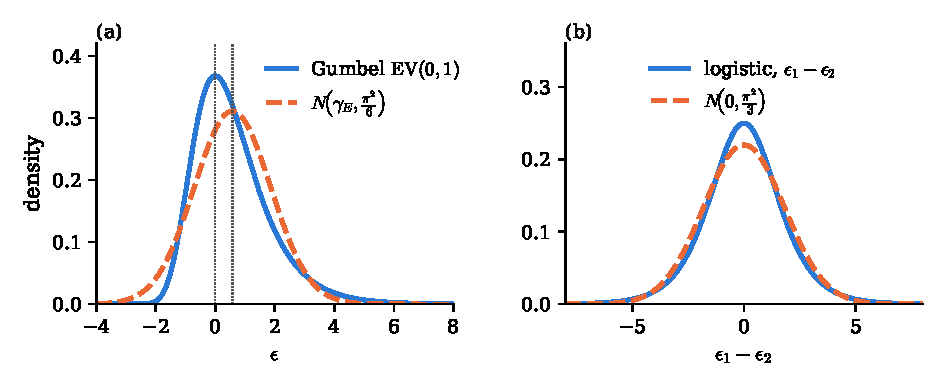
\includegraphics[width=\textwidth]{figures/appB/gumbel_logistic.pdf}
\caption{Panel (a): the standard Gumbel density and the normal density with the same mean $\gamma_E$ and
variance $\frac{\pi^2}{6}$. The dotted lines mark the mode $0$ and the mean $\gamma_E$. The Gumbel is skewed to the
right. Panel (b): the standard logistic density, which is the density of the difference of two independent
standard Gumbels (\cref{prop:B-logistic}), and the normal density with mean $0$ and variance
$\frac{\pi^2}{3}$. The logistic is symmetric and close to the normal, with slightly fatter tails.}\label{fig:B-gumbel}
\end{figure}

\subsection{Max-stability and the logit formula}\label{sec:B-maxstable}

The Gumbel family is closed under maxima with a common scale. This single property delivers the logit
formula, the log-sum and the nested logit.

\begin{proposition}[Max-stability]\label{prop:B-maxstable}
Let $\epsilon_0, \dots, \epsilon_J$ be independent $\mathrm{EV}(0, b)$ and let $\delta_0, \dots, \delta_J$ be constants. Then
\begin{equation}\label{eq:B-maxstable}
\max_j(\delta_j + \epsilon_j) \sim \mathrm{EV}\left(b\ln\sum_{j = 0}^Je^{\frac{\delta_j}{b}},\ b\right).
\end{equation}
\end{proposition}

\Cref{lem:06-maxstable} proves the case $b = 1$, and the text after it extends the proof to scale $b$. The proof
multiplies the independent Gumbel CDFs $\exp(-e^{-\frac{x - \delta_j}{b}})$ and collects the exponents.

\begin{proposition}[Logistic differences]\label{prop:B-logistic}
If $\epsilon_1$ and $\epsilon_2$ are independent standard Gumbels, then $\epsilon_1 - \epsilon_2$ has the standard
logistic distribution,
\begin{equation*}
\Pr(\epsilon_1 - \epsilon_2 \leq x) = \frac{1}{1 + e^{-x}},
\end{equation*}
with density $\frac{e^{-x}}{(1 + e^{-x})^2}$, mean zero and variance $\frac{\pi^2}{3}$.
\end{proposition}

\Cref{lem:06-logistic} proves the result by conditioning on $\epsilon_2$ and substituting $t = e^{-\epsilon_2}$.

\begin{theorem}[Multinomial logit, \citealp{McFadden1974}]\label{thm:B-logit}
Let $u_{ij} = \delta_j + \epsilon_{ij}$ with $\epsilon_{i0}, \dots, \epsilon_{iJ}$ independent standard Gumbels. Then
\begin{equation}\label{eq:B-logit}
s_j(\delta) = \frac{e^{\delta_j}}{\sum_{k = 0}^Je^{\delta_k}} = \frac{e^{\delta_j}}{1 + \sum_{k = 1}^Je^{\delta_k}}
\quad\text{when } \delta_0 = 0 .
\end{equation}
With $\mathrm{EV}(0, b)$ shocks,
\begin{equation*}
s_j(\delta) = \frac{\exp\left(\frac{\delta_j}{b}\right)}{\sum_{k = 0}^J\exp\left(\frac{\delta_k}{b}\right)} .
\end{equation*}
\end{theorem}

\citet[eqs.~3.14--3.15, pp.~1411--1412]{McFadden1984} states the result and notes that it follows by a
straightforward integration. \Cref{prop:06-logit} gives two proofs. The first carries out that integration,
conditioning on $\epsilon_{ij}$ and substituting $t = e^{-\epsilon_{ij}}$. The second combines the two previous
propositions. By \cref{prop:B-maxstable}, the best rival utility is $\ln\sum_{k \neq j}e^{\delta_k}$ plus a standard
Gumbel shock independent of $\epsilon_{ij}$. By \cref{prop:B-logistic}, the difference of the two shocks is logistic.

The scale $b$ governs how deterministic choice is. As $b \to 0$, the alternative with the highest $\delta_j$
is chosen with probability one. As $b \to \infty$, all shares tend to $\frac{1}{J + 1}$.

\begin{proposition}[The chosen maximum]\label{prop:B-chosen-max}
In the logit model of \cref{thm:B-logit}, with $\Lambda = \sum_{k = 0}^Je^{\delta_k}$,
\begin{equation}\label{eq:B-chosen-max}
\Pr\Big(\max_k u_{ik} \leq x,\ j \text{ chosen}\Big) = s_j\exp\big(-e^{-x}\Lambda\big).
\end{equation}
Hence the distribution of the maximal utility conditional on choosing $j$ is $\mathrm{EV}(\ln\Lambda, 1)$ for
every $j$, the identity of the chosen alternative is independent of the maximal utility, and
\begin{equation}\label{eq:B-selection}
\E\big[\epsilon_{ij} \mid j \text{ chosen}\big] = \gamma_E - \ln s_j .
\end{equation}
\end{proposition}

\begin{proof}
By \cref{prop:06-logsum}, the joint probability factors as
$s_j\Pr(\max_ku_{ik} \leq x)$, which is \eqref{eq:06-maxindep}. Its proof repeats the direct integration of \cref{prop:06-logit} with the extra
restriction $\delta_j + \epsilon_{ij} \leq x$. By \cref{prop:B-maxstable}, $\Pr(\max_ku_{ik} \leq x) = \exp(-e^{-x}\Lambda)$,
which gives \eqref{eq:B-chosen-max}. Dividing by $s_j$ gives the conditional CDF $\exp(-e^{-(x - \ln\Lambda)})$,
which does not depend on $j$. Its mean is $\ln\Lambda + \gamma_E$. On the event that $j$ is chosen, $\epsilon_{ij} = \max_ku_{ik} - \delta_j$, so
$\E[\epsilon_{ij} \mid j \text{ chosen}] = \ln\Lambda + \gamma_E - \delta_j = \gamma_E - \ln s_j$.
\end{proof}

Equation \eqref{eq:B-selection} quantifies selection. Consumers who choose a product with a small share have,
on average, a large taste shock for it. Corrections for selection in models that combine a discrete choice
with a continuous outcome use this formula \citep{DubinMcFadden1984}. The independence of the winner and
the winning value is also the key step in the nest-by-nest derivation of the nested logit (\cref{prop:B-cardell}).

\emph{Independence of irrelevant alternatives} (IIA) is the property that the ratio of two choice
probabilities does not depend on any third alternative. From \eqref{eq:B-logit},
\begin{equation}\label{eq:B-iia}
\frac{s_j}{s_k} = e^{\delta_j - \delta_k},
\end{equation}
which is equation (3.17) of \citet[p.~1413]{McFadden1984}. Two implications follow. Choice probabilities
on a smaller or larger choice set are obtained by deleting or adding terms in the denominator. The cross
elasticity of every alternative with respect to an attribute of $k$ is the same \citep[p.~1414]{McFadden1984}.
The classic illustration is the red bus and the blue bus. A commuter chooses between a car and a red bus
with equal mean utilities, so each share is $\frac{1}{2}$. Add a blue bus identical to the red one. IIA keeps
the ratio of car to red bus at one, so logit predicts shares of $\frac{1}{3}$ each. Common sense predicts
$\frac{1}{2}$ for the car and $\frac{1}{4}$ for each bus. IIA follows from the logit specification, in which
the shocks are independent standard Gumbels. Independence alone does not deliver it, and probit choice
probabilities do not satisfy IIA \citep[Section~5.4, p.~108]{Train2009}. Take three alternatives with
independent standard normal shocks and $\delta = (1, 0, \delta_3)$. The ratio $\frac{s_1}{s_2}$ is $3.17$ at
$\delta_3 = -5$ and $3.46$ at $\delta_3 = 0$. Under logit the ratio would equal $e \approx 2.72$ at every
$\delta_3$, so the probit ratio depends on the third alternative. I.i.d.\ normal shocks still share the red bus
failure. By symmetry they give the car and each bus a share of $\frac{1}{3}$, because they contain no notion of similarity
between products. More generally, any shock that is i.i.d.\ across alternatives gives two products with equal
shares the same cross elasticity with respect to the price of a third (\cref{rem:07-berry-iid}). The remedy is
correlation across alternatives, through nests (\cref{sec:B-gev}) or random coefficients (\cref{ch:blp}). IIA can be tested by comparing estimates from the full and a restricted choice set
\citep{HausmanMcFadden1984}.

\subsection{Expected maximum utility and consumer surplus}\label{sec:B-logsum}

\begin{proposition}[Log-sum formula]\label{prop:B-logsum}
In the logit model of \cref{thm:B-logit},
\begin{equation}\label{eq:B-logsum}
\mathcal{W}(\delta) = \E\Big[\max_j(\delta_j + \epsilon_{ij})\Big] = \ln\sum_{j = 0}^Je^{\delta_j} + \gamma_E = \ln\Lambda + \gamma_E .
\end{equation}
\end{proposition}

\Cref{prop:06-logsum} proves the formula. By \cref{prop:B-maxstable} with $b = 1$ the maximum is
$\mathrm{EV}(\ln\Lambda, 1)$, and its mean is $\ln\Lambda + \gamma_E$ by \cref{prop:B-gumbel-moments}.

The quantity $\ln\Lambda$ is the \emph{inclusive value} of the choice set. The next theorem shows that the
gradient of the expected maximum utility is the vector of choice probabilities in every additive random
utility model. The logit is one instance.

\begin{theorem}[Williams-Daly-Zachary, \citealp{Williams1977, DalyZachary1978, McFadden1981}]\label{thm:B-wdz}
Under \cref{ass:B-arum}, the function $\mathcal{W}(\delta) = \E[\max_k(\delta_k + \epsilon_{ik})]$ is finite, convex and
continuously differentiable, and
\begin{equation}\label{eq:B-wdz}
\frac{\partial\mathcal{W}(\delta)}{\partial\delta_j} = s_j(\delta), \qquad j = 0, \dots, J .
\end{equation}
\end{theorem}

\Cref{thm:06-wdz} proves finiteness, convexity and \eqref{eq:B-wdz}. Off the tie set, which has probability
zero, a small change in $\delta_j$ does not change the maximizer. The pointwise derivative of
$\max_k(\delta_k + \epsilon_k)$ is therefore the indicator that $j$ is chosen. The difference quotients are bounded by
one, and dominated convergence moves the derivative inside the expectation. The one addition is continuity of
the derivative.

\begin{proof}[Proof of continuous differentiability]
Let $\delta' \to \delta$. The indicator of $A_j(\delta')$ converges to the indicator of $A_j(\delta)$ at every
$\epsilon$ off the boundary of $A_j(\delta)$, which is a null set. Indicators are bounded by one, so dominated
convergence gives $s_j(\delta') \to s_j(\delta)$. The gradient of $\mathcal{W}$ is therefore continuous.
\end{proof}

The theorem is an envelope theorem: the derivative of a maximum with respect to a parameter is the
derivative of the chosen term (\cref{sec:B-envelope}). Four consequences follow.
\begin{enumerate}[label=(\alph*)]
\item (Symmetry) Where $s$ is differentiable, $\frac{\partial s_j}{\partial\delta_k} = \frac{\partial^2\mathcal{W}}{\partial\delta_k\partial\delta_j}
  = \frac{\partial s_k}{\partial\delta_j}$ in every additive random utility model.
\item (Positive semidefiniteness) The Jacobian $\frac{\partial s}{\partial\delta^\T}$ is the Hessian of a convex function,
  hence positive semidefinite. In particular $\frac{\partial s_j}{\partial\delta_j} \geq 0$.
\item (Translation) $\mathcal{W}(\delta + c\mathbf{1}) = \mathcal{W}(\delta) + c$. Differentiating in $c$ gives $\sum_js_j = 1$.
\item (Roy's identity) Let $\delta_j = \alpha(y - p_j) + \tilde\delta_j$ for $j \geq 1$ and $\delta_0 = \alpha y$. Then
  $\frac{\partial\mathcal{W}}{\partial p_j} = -\alpha s_j$ and $\frac{\partial\mathcal{W}}{\partial y} = \alpha$, so
  $s_j = -\frac{\partial\mathcal{W}}{\partial p_j}\left[\frac{\partial\mathcal{W}}{\partial y}\right]^{-1}$, the analogue of
  \eqref{eq:B-roy} with $\mathcal{W}$ as the indirect utility function.
\end{enumerate}
For the logit, $\frac{\partial}{\partial\delta_j}\ln\sum_ke^{\delta_k} = \frac{e^{\delta_j}}{\sum_ke^{\delta_k}} = s_j$, which checks
\eqref{eq:B-wdz} against \eqref{eq:B-logsum}.

\begin{proposition}[Logit consumer surplus, \citealp{SmallRosen1981}]\label{prop:B-cs}
Let $u_{ij} = \alpha(y_i - p_j) + \tilde\delta_j + \epsilon_{ij}$ for $j \geq 1$ and $u_{i0} = \alpha y_i + \epsilon_{i0}$, with
independent standard Gumbel shocks and $\alpha > 0$. Write $\delta_j = \tilde\delta_j - \alpha p_j$. Then the expected
consumer surplus in money is
\begin{equation}\label{eq:B-cs}
CS_i = \frac{1}{\alpha}\ln\Big(1 + \sum_{k = 1}^Je^{\delta_k}\Big) + C,
\end{equation}
where $C$ is a constant that cancels in comparisons. For a change from $\delta^0$ to $\delta^1$, the
expectation of each consumer's exact compensating variation is
$\frac{1}{\alpha}\left(\ln\Lambda^1 - \ln\Lambda^0\right)$, where $\Lambda^s = 1 + \sum_{k \geq 1}e^{\delta_k^s}$.
\end{proposition}

\Cref{sec:06-arum} proves the general formula \eqref{eq:06-smallrosen}, and \cref{sec:06-logsum} evaluates it
for the logit. Income enters every alternative with the same coefficient, so each consumer's compensating
variation is $\frac{1}{\alpha}$ times the change in her maximal utility. Taking expectations with
\cref{prop:B-logsum} gives the result. This $CV$ is a gain measure, positive when the consumer is better off,
which is the opposite sign convention to \cref{def:B-cv-ev}.

The utility is quasi-linear in income, so \cref{prop:B-quasilinear} applies. No income effects arise, and
the compensating and equivalent variations coincide. With market size $M$, the aggregate change is
$\frac{M}{\alpha}(\ln\Lambda^1 - \ln\Lambda^0)$. With random coefficients, each consumer type $i$ has its own price
coefficient $\alpha_i$ and inclusive value $\ln\Lambda_i$, and
$\Delta CS = M\int\frac{1}{\alpha_i}(\ln\Lambda_i^1 - \ln\Lambda_i^0)\,\dd F(\nu_i)$ (\cref{ch:blp}, \cref{ch:mergers}).

\begin{corollary}[Value of a product]\label{cor:B-value-product}
In the setting of \cref{prop:B-cs}:
\begin{enumerate}[label=(\roman*)]
\item Adding a product $n$ with mean utility $\delta_n$ raises expected surplus by
\begin{equation}\label{eq:B-value-new}
\Delta CS = \frac{1}{\alpha}\ln\left(1 + \frac{e^{\delta_n}}{\Lambda^0}\right) = -\frac{1}{\alpha}\ln(1 - s_n),
\end{equation}
  where $s_n = \frac{e^{\delta_n}}{\Lambda^0 + e^{\delta_n}}$ is the share of the product after its introduction.
  Removing a product with share $s_n$ costs the same amount.
\item A perfect clone of an existing product $j$, with $\delta_n = \delta_j$, adds
  $\frac{1}{\alpha}\ln\left(1 + \frac{e^{\delta_j}}{\Lambda^0}\right) > 0$.
\item With $J$ identical products of mean utility $\delta$, $CS = \frac{1}{\alpha}\ln(1 + Je^\delta) + C$, which grows
  like $\frac{1}{\alpha}\ln J$ without bound.
\end{enumerate}
\end{corollary}

\begin{proof}
(i) $\Lambda^1 = \Lambda^0 + e^{\delta_n}$, so $\ln\Lambda^1 - \ln\Lambda^0 = \ln\left(1 + \frac{e^{\delta_n}}{\Lambda^0}\right)$. Since
$\frac{\Lambda^0}{\Lambda^1} = 1 - s_n$, the same quantity equals $-\ln(1 - s_n)$. (ii) Set $\delta_n = \delta_j$ in (i).
(iii) Here $\Lambda = 1 + Je^\delta$ and $\ln(1 + Je^\delta) = \ln J + \delta + \ln(1 + \frac{e^{-\delta}}{J})$.
\end{proof}

The corollary is the formal content of the statement that the logit shock never exhausts the product
space. Every product arrives with its own independent taste draw, so every product, even a duplicate,
attracts consumers who value it highly and adds surplus. The same feature bounds logit markups below by
$\frac{1}{\alpha}$ (\cref{prop:B-logit-markups}). It biases upward the estimated value of new goods and the
markups in crowded markets (\cref{ch:discrete}, \cref{ch:newgoods}). The mirror image concerns data. The model
predicts a positive share for every product, so the direct inversion of observed shares, $\ln s_j^{obs} - \ln s_0^{obs}$, is
undefined for a product with zero observed sales. The zero is still informative. If $M$ consumers choose
independently, the probability of observing no sale of $j$ is $(1 - s_j)^M$, which falls as the model share
$s_j$ rises. A likelihood for sales counts, or another estimator that models the sampling of shares, can
therefore use zeros \citep{GandhiLuShi2023}. If the shocks represent mistakes or
psychological biases rather than tastes, the log-sum counts them as welfare. The pure characteristics model
removes the shock altogether, and the nested logit shrinks the value of a clone as within-nest correlation
rises (\cref{rem:B-nl-clone}).

In computation, $\ln\sum_{k = 0}^Je^{\delta_k}$ overflows when some $\delta_k$ is large. Let
$c = \max\{0, \max_k\delta_k\}$, where the zero is the outside good. Then evaluate
\begin{equation}\label{eq:B-logsumexp}
\ln\sum_{k = 0}^Je^{\delta_k} = c + \ln\sum_{k = 0}^Je^{\delta_k - c},
\end{equation}
in which every exponent is at most zero. The same shift stabilizes the share formula.

\subsection{Logit derivatives, Jacobians and markups}\label{sec:B-logit-algebra}

With $s_j = \frac{e^{\delta_j}}{\Lambda}$ and $\Lambda = 1 + \sum_ke^{\delta_k}$, the quotient rule gives the derivatives
that \cref{ex:B-logit-jacobian} computed. We collect them in three equivalent forms,
\begin{equation}\label{eq:B-logit-deriv}
\frac{\partial s_j}{\partial\delta_k} = s_j\big(\indic\{j = k\} - s_k\big),
\qquad
\frac{\partial\ln s_j}{\partial\delta_k} = \indic\{j = k\} - s_k,
\qquad
\frac{\partial s}{\partial\delta^\T} = \diag(s) - ss^\T,
\end{equation}
where $s = (s_1, \dots, s_J)^\T$ collects the inside shares. The Jacobian is symmetric, as \cref{thm:B-wdz}
requires. Its row sums are $\sum_{k \geq 1}\frac{\partial s_j}{\partial\delta_k} = s_j(1 - \sum_ks_k) = s_js_0 > 0$. The
derivative with respect to the outside good is $-s_js_0$, so the full row sums to zero, as translation
invariance requires (\cref{cor:B-translation}). The Jacobian is invertible, and the Sherman-Morrison formula gives
its inverse $\diag(\frac{1}{s_1}, \dots, \frac{1}{s_J}) + \frac{1}{s_0}\mathbf{1}\mathbf{1}^\T$ in
\eqref{eq:B-logit-jacobian-inverse}. Inverting the shares themselves is easier still:
$\frac{s_j}{s_0} = e^{\delta_j}$ gives $\delta_j = \ln s_j - \ln s_0$, the inversion of \citet{Berry1994} that
\cref{ch:logit} turns into a linear instrumental variables regression.

With $\delta_j = \tilde\delta_j - \alpha p_j$, the chain rule gives the price derivatives
$\frac{\partial s_j}{\partial p_j} = -\alpha s_j(1 - s_j)$ and $\frac{\partial s_j}{\partial p_k} = \alpha s_js_k$. The own-price
elasticity and the cross elasticities are
\begin{equation}\label{eq:B-logit-elast}
\varepsilon_j = -\frac{\partial s_j}{\partial p_j}\frac{p_j}{s_j} = \alpha p_j(1 - s_j),
\qquad
\varepsilon_{jk} = \frac{\partial s_j}{\partial p_k}\frac{p_k}{s_j} = \alpha p_ks_k \quad (k \neq j).
\end{equation}
The own elasticity is nearly proportional to price when shares are small, so the model predicts that
expensive products face the most elastic demand. The cross elasticity with respect to $p_k$ is the same for
every $j$, whatever the similarity of $j$ and $k$. The diversion ratio from $j$ to $k$ is
\begin{equation}\label{eq:B-logit-diversion}
D_{jk} = -\frac{\partial s_k}{\partial p_j}\left[\frac{\partial s_j}{\partial p_j}\right]^{-1} = \frac{\alpha s_js_k}{\alpha s_j(1 - s_j)} = \frac{s_k}{1 - s_j},
\qquad
D_{j0} = \frac{s_0}{1 - s_j} .
\end{equation}
Customers who leave $j$ spread over the other alternatives in proportion to their shares, and the
diversion ratios sum to one.

\begin{proposition}[Logit markups]\label{prop:B-logit-markups}
Let firms set prices in a Bertrand-Nash equilibrium with constant marginal costs and logit demand, and write
$m_j = p_j - mc_j$.
\begin{enumerate}[label=(\roman*)]
\item A single-product firm sets $m_j = \frac{1}{\alpha(1 - s_j)}$.
\item A firm $f$ that owns the products $\mathcal{J}_f$, with combined share $S_f = \sum_{k \in \mathcal{J}_f}s_k$, sets
  the common markup $m_j = m_f = \frac{1}{\alpha(1 - S_f)}$ on all its products.
\item A single owner of all inside goods sets the common markup $\frac{1}{\alpha s_0}$.
\end{enumerate}
In every case $m_j > \frac{1}{\alpha}$.
\end{proposition}

\begin{proof}
(ii) The profit of firm $f$ is $\sum_{k \in \mathcal{J}_f}m_ks_k(p)$. For $j \in \mathcal{J}_f$, the first-order condition is
\begin{equation*}
0 = s_j + \sum_{k \in \mathcal{J}_f}m_k\frac{\partial s_k}{\partial p_j}
= s_j - \alpha m_js_j(1 - s_j) + \sum_{k \in \mathcal{J}_f, k \neq j}\alpha m_ks_ks_j
= s_j\Big[1 - \alpha m_j + \alpha\sum_{k \in \mathcal{J}_f}m_ks_k\Big].
\end{equation*}
Dividing by $s_j > 0$ gives $m_j = \frac{1}{\alpha} + \sum_{k \in \mathcal{J}_f}m_ks_k$. The right side does not depend
on $j$, so all products of the firm carry the same markup $m_f$. Substituting $m_k = m_f$ gives
$m_f = \frac{1}{\alpha} + S_fm_f$, hence $m_f = \frac{1}{\alpha(1 - S_f)}$. (i) is the case $\mathcal{J}_f = \{j\}$. (iii) is the
case $S_f = 1 - s_0$. Each markup exceeds $\frac{1}{\alpha}$ because $S_f < 1$.
\end{proof}

\Cref{ex:B-logit-jacobian} reaches the same three formulas from the matrix condition
$m = -(\Omega \odot \Delta^\T)^{-1}s$, by inverting each block of the logit Jacobian with the Sherman-Morrison formula.

The first-order condition of a single-product firm is also sufficient. Write
$\frac{\partial\pi_j}{\partial p_j} = s_j\,g(m_j)$ with $g(m) = 1 - \alpha m(1 - s_j)$, where $s_j$ depends on $m$ through
$p_j$. For $m \leq 0$ we have $g > 0$. For $m > 0$, $g$ is strictly decreasing, because both $\alpha m$ and
$1 - s_j$ rise with $p_j$, and $g \to -\infty$ as $m \to \infty$. The derivative of profit therefore changes sign
exactly once, from positive to negative, and the stationary point is the unique maximizer. The best
response has a closed form in terms of the Lambert function.

\begin{lemma}[Lambert function, \citealp{CorlessEtAl1996}]\label{lem:B-lambert}
For every $z \geq 0$, the equation $we^w = z$ has exactly one solution $w \geq 0$, denoted $W_0(z)$. The
function $W_0$ is strictly increasing on $[0, \infty)$, with $W_0(0) = 0$ and $W_0(e) = 1$, and for $z > 0$
\begin{equation}\label{eq:B-lambert-deriv}
W_0'(z) = \frac{W_0(z)}{z\,(1 + W_0(z))} .
\end{equation}
\end{lemma}

\begin{proof}
The map $g(w) = we^w$ is continuous on $[0, \infty)$ with $g(0) = 0$, $g(w) \to \infty$ and
$g'(w) = (1 + w)e^w > 0$. By the intermediate value theorem and strict monotonicity, each $z \geq 0$ has
exactly one preimage, and the inverse is strictly increasing. Since $1\cdot e^1 = e$, $W_0(e) = 1$. By the
inverse function theorem,
\begin{equation*}
W_0'(z) = \frac{1}{g'(W_0(z))} = \frac{1}{(1 + W_0(z))e^{W_0(z)}} = \frac{W_0(z)}{z\,(1 + W_0(z))},
\end{equation*}
where the last step uses $e^{W_0(z)} = \frac{z}{W_0(z)}$ for $z > 0$.
\end{proof}

The principal branch extends to $z \geq -\frac{1}{e}$, but we only need $z > 0$. Standard numerical libraries
evaluate it.

\begin{proposition}[Logit best response]\label{prop:B-logit-br}
Let firm $j$ sell one product with logit demand, $\delta_j = \tilde\delta_j - \alpha p_j$, and constant marginal cost
$mc_j$. Define the mean utility at marginal-cost pricing, $v_j = \tilde\delta_j - \alpha mc_j$, and the part of the
logit denominator that rivals control, $\Lambda_{-j} = 1 + \sum_{l \neq j}e^{\delta_l}$. Then the unique best response
to the rivals' prices is
\begin{equation}\label{eq:B-logit-br-closed}
BR_j(p_{-j}) = mc_j + \frac{1}{\alpha}\left[1 + W_0\left(\frac{e^{v_j - 1}}{\Lambda_{-j}}\right)\right] .
\end{equation}
At the best response, with $W_0$ evaluated at $z_j = \frac{e^{v_j - 1}}{\Lambda_{-j}}$,
\begin{equation}\label{eq:B-br-identities}
s_j = \frac{W_0(z_j)}{1 + W_0(z_j)}, \qquad \frac{e^{\delta_l}}{\Lambda_{-j}} = \frac{s_l}{1 - s_j} \quad (l \neq j).
\end{equation}
For a multiproduct firm $f$ with $E_f = \sum_{k \in \mathcal{J}_f}e^{v_k}$ and $\Lambda_{-f} = 1 + \sum_{l \notin \mathcal{J}_f}e^{\delta_l}$,
the best-response common markup is $m_f = \frac{1}{\alpha}\left[1 + W_0\left(\frac{E_fe^{-1}}{\Lambda_{-f}}\right)\right]$.
\end{proposition}

\begin{proof}
By \cref{prop:B-logit-markups} and the single-crossing argument above, the best response is the unique
solution of $\alpha m_j(1 - s_j) = 1$. Write $\delta_j = v_j - \alpha m_j$ and
$1 - s_j = \frac{\Lambda_{-j}}{\Lambda_{-j} + e^{\delta_j}}$. The condition becomes
\begin{equation*}
\alpha m_j\Lambda_{-j} = \Lambda_{-j} + e^{v_j - \alpha m_j}
\quad\Longleftrightarrow\quad
(\alpha m_j - 1)\Lambda_{-j} = e^{v_j - \alpha m_j} .
\end{equation*}
Let $w = \alpha m_j - 1$. Then $w\Lambda_{-j} = e^{v_j - 1 - w}$, that is,
\begin{equation*}
we^w = \frac{e^{v_j - 1}}{\Lambda_{-j}} = z_j > 0 .
\end{equation*}
Any solution has $w > 0$, because the right side is positive. By \cref{lem:B-lambert}, $w = W_0(z_j)$, and
$m_j = \frac{1 + W_0(z_j)}{\alpha}$, which is \eqref{eq:B-logit-br-closed}. At the best response the first-order condition
gives $1 - s_j = \frac{1}{\alpha m_j} = \frac{1}{1 + W_0(z_j)}$, which yields the first identity in
\eqref{eq:B-br-identities}. For the second, $\frac{\Lambda_{-j}}{\Lambda} = 1 - s_j$ with $\Lambda = \Lambda_{-j} + e^{\delta_j}$, so
$\frac{e^{\delta_l}}{\Lambda_{-j}} = \frac{e^{\delta_l}}{\Lambda}\cdot\frac{\Lambda}{\Lambda_{-j}} = \frac{s_l}{1 - s_j}$. For the multiproduct
firm, the common-markup condition $\alpha m_f(1 - S_f) = 1$ with
$1 - S_f = \frac{\Lambda_{-f}}{\Lambda_{-f} + E_fe^{-\alpha m_f}}$ gives $(\alpha m_f - 1)\Lambda_{-f} = E_fe^{-\alpha m_f}$, and the same
substitution yields $we^w = \frac{E_fe^{-1}}{\Lambda_{-f}}$.
\end{proof}

The best response rises with every rival price, because $\Lambda_{-j}$ falls and $W_0$ is increasing. Prices are
strategic complements. \Cref{sec:B-fixedpoint} differentiates \eqref{eq:B-logit-br-closed} with
\eqref{eq:B-lambert-deriv} and \eqref{eq:B-br-identities} to show that best-response iteration is a contraction, so
the logit pricing equilibrium is unique.

\begin{remark}[Mixed logit]\label{rem:B-mixed}
In the random-coefficients (mixed) logit, conditional on the consumer's taste draw $\nu_i$ the choice
probabilities $s_{ij}$ are logit. The formulas of this subsection for choice probabilities, price derivatives,
elasticities and diversion ratios therefore hold consumer by consumer, with $s_{ij}$ and $\alpha_i$ in place of $s_j$
and $\alpha$. Aggregate shares and derivatives are integrals, for example
$\frac{\partial s_j}{\partial p_k} = \int\alpha_is_{ij}\big(s_{ik} - \indic\{j = k\}\big)\,\dd F(\nu_i)$, where differentiation
under the integral is justified by \cref{prop:B-leibniz}. Aggregate cross derivatives are large when the same
consumers are likely to buy both products, so substitution depends on characteristics. The pricing results
(\cref{prop:B-logit-markups,prop:B-logit-br}) do not hold consumer by consumer. A firm charges one price to all
consumers, so its first-order condition sets the integral of the consumer-level terms to zero, and each term need
not vanish. Markups solve $m = -(\Omega \odot \Delta^\T)^{-1}s$ with the aggregate derivatives, and they are no longer
common within a firm. \citet{McFaddenTrain2000} show that any random utility model can be approximated
arbitrarily well by a mixed logit (\cref{ch:blp}).
\end{remark}

\subsection{Representative-consumer foundations}\label{sec:B-entropy}

The logit can also be derived from a single consumer who likes variety.

\begin{proposition}[Entropy representative consumer, \citealp{AndersonDePalmaThisse1988, AndersonDePalmaThisse1992}]\label{prop:B-entropy}
Let $\delta_0, \dots, \delta_J$ be given, with $\delta_j = \tilde\delta_j - \alpha p_j$ and $\delta_0 = 0$. The problem
\begin{equation}\label{eq:B-entropy}
\max_{q_0, \dots, q_J \geq 0}\ \sum_{j = 0}^J\delta_jq_j - \sum_{j = 0}^Jq_j\ln q_j
\qquad\text{subject to}\qquad \sum_{j = 0}^Jq_j = 1
\end{equation}
has the unique solution $q_j = \frac{e^{\delta_j}}{\sum_ke^{\delta_k}}$, the logit shares. Its maximized value is
$\ln\sum_ke^{\delta_k}$.
\end{proposition}

\Cref{prop:04-logit-entropy} proves the result. Strict concavity of $-q\ln q$ gives a unique maximizer, its
infinite slope at zero makes the maximizer interior, and the first-order conditions
$\delta_j - \ln q_j - 1 - \lambda = 0$ give the logit shares.

The entropy term $-\sum_jq_j\ln q_j$ rewards spreading consumption across products, a taste for variety. The
maximized value equals the log-sum of \eqref{eq:B-logsum} without the constant $\gamma_E$, so the representative
consumer and the population of random-utility consumers agree on welfare. In the language of convex
analysis, the log-sum is the convex conjugate of negative entropy on the simplex. Weighting the entropy
term by $b > 0$ gives the logit with scale $b$, and as $b \to 0$ the consumer buys only the product with
the highest $\delta_j$.

\begin{remark}[Logit and CES]\label{rem:B-logit-ces}
CES expenditure shares are logit shares in log prices. With the CES price index
$P^{1 - \sigma_{\mathrm{CES}}} = \sum_ka_kp_k^{1 - \sigma_{\mathrm{CES}}}$, the budget share of good $j$ is
$w_j = \frac{a_jp_j^{1 - \sigma_{\mathrm{CES}}}}{\sum_ka_kp_k^{1 - \sigma_{\mathrm{CES}}}}$ (\cref{ch:diffprod}). Setting
$\delta_j = \ln a_j - (\sigma_{\mathrm{CES}} - 1)\ln p_j$ in \eqref{eq:B-logit} without an outside good gives
\begin{equation*}
s_j = \frac{e^{\ln a_j - (\sigma_{\mathrm{CES}} - 1)\ln p_j}}{\sum_ke^{\ln a_k - (\sigma_{\mathrm{CES}} - 1)\ln p_k}}
= \frac{a_jp_j^{1 - \sigma_{\mathrm{CES}}}}{\sum_ka_kp_k^{1 - \sigma_{\mathrm{CES}}}} = w_j .
\end{equation*}
The coefficient on log price, $\sigma_{\mathrm{CES}} - 1$, plays the role of the logit price coefficient, and the
CES inherits IIA. \citet{AndersonDePalmaThisse1987} give a discrete-choice foundation. Suppose each consumer
buys one variety and spends all income $y$ on it, with conditional indirect utility
$\ln y - \ln p_j + \ln\tilde a_j + \mu\epsilon_{ij}$ and standard Gumbel shocks scaled by $\mu > 0$. The choice
probabilities are logit in $\frac{\ln\tilde a_j - \ln p_j}{\mu}$, and expected demand for $j$ is the choice
probability times $\frac{y}{p_j}$. This is CES demand with $\sigma_{\mathrm{CES}} = 1 + \frac{1}{\mu}$ and weights
$a_j = \tilde a_j^{\sigma_{\mathrm{CES}} - 1}$. The subscript keeps $\sigma$ free for the nesting parameter.
\end{remark}

\subsection{Generalized extreme value models}\label{sec:B-gev}

The generalized extreme value (GEV) class of \citet{McFadden1978} keeps closed-form choice probabilities
while allowing the shocks to be correlated across alternatives. Its key object is a generating function.

\begin{theorem}[GEV models, \citealp{McFadden1978}]\label{thm:B-gev}
Let $H : \R^{J+1}_+ \to \R_+$ satisfy three conditions:
\begin{enumerate}[label=(G\arabic*)]
\item $H$ is nonnegative and homogeneous of degree one.
\item $H(y_0, \dots, y_J) \to \infty$ as any single argument $y_j \to \infty$.
\item For every set of $m$ distinct arguments, the mixed partial derivative of $H$ with respect to them is
  nonnegative when $m$ is odd and nonpositive when $m$ is even.
\end{enumerate}
Then $F(\epsilon_0, \dots, \epsilon_J) = \exp\{-H(e^{-\epsilon_0}, \dots, e^{-\epsilon_J})\}$ is a multivariate extreme value CDF.
Let $u_{ij} = \delta_j + \epsilon_{ij}$ with $\epsilon_i \sim F$ and $y_j = e^{\delta_j}$. Then:
\begin{enumerate}[label=(\roman*)]
\item $\Pr(\max_ju_{ij} \leq x) = \exp\{-e^{-x}H(y)\}$, so the maximal utility is $\mathrm{EV}(\ln H(y), 1)$.
  Expected maximum utility is
  \begin{equation}\label{eq:B-gev-W}
  \mathcal{W}(\delta) = \ln H\big(e^{\delta_0}, \dots, e^{\delta_J}\big) + \gamma_E .
  \end{equation}
\item The choice probabilities are
  \begin{equation}\label{eq:B-gev-shares}
  s_j = \frac{\partial\ln H(e^{\delta_0}, \dots, e^{\delta_J})}{\partial\delta_j} = \frac{y_jH_j(y)}{H(y)},
  \end{equation}
  where $H_j$ is the partial derivative of $H$ with respect to its $j$-th argument.
\end{enumerate}
\end{theorem}

\citet[eqs.~3.29--3.31, p.~1421]{McFadden1984} states the theorem in this form. The first claim, that (G1) to
(G3) make $F$ a valid distribution function, is due to \citet{McFadden1978}. Condition (G3) makes the mixed
partial derivative of $F$ of order $J + 1$, its density, nonnegative. Condition (G2) makes each marginal CDF
vanish as its argument tends to $-\infty$. \Cref{thm:06-gev} proves (i) and (ii). Part (i) follows from
homogeneity, since $F(x - \delta_0, \dots, x - \delta_J) = \exp\{-H(e^{-x}y)\} = \exp\{-e^{-x}H(y)\}$. That proof
derives (ii) by direct integration. Part (ii) also follows from (i) in one line. The distribution $F$ satisfies
\cref{ass:B-arum}, so \cref{thm:B-wdz} applied to \eqref{eq:B-gev-W} gives
$s_j = \frac{H_j(y)}{H(y)}\cdot\frac{\partial y_j}{\partial\delta_j} = \frac{y_jH_j(y)}{H(y)}$.

By Euler's theorem, $\sum_jy_jH_j(y) = H(y)$, so the shares in \eqref{eq:B-gev-shares} sum to one. Part (i)
explains a remark of \citet[p.~1425]{McFadden1984}. The generating function can be read as a measure of social
utility, because its logarithm is expected maximum utility up to a constant.

\begin{example}[Logit as a GEV model]\label{ex:B-gev-logit}
With $H(y) = \sum_jy_j$, $H_j = 1$ and \eqref{eq:B-gev-shares} gives $s_j = \frac{y_j}{\sum_ky_k}$, the logit. The
generating function $H(y) = \left(\sum_jy_j^{\frac{1}{\lambda}}\right)^\lambda$ with $0 < \lambda \leq 1$
\citep[eq.~3.32]{McFadden1984} also gives a logit. Here
$H_j = \left(\sum_ky_k^{\frac{1}{\lambda}}\right)^{\lambda - 1}y_j^{\frac{1}{\lambda} - 1}$, so
$s_j = \frac{y_j^{\frac{1}{\lambda}}}{\sum_ky_k^{\frac{1}{\lambda}}} = \frac{e^{\frac{\delta_j}{\lambda}}}{\sum_ke^{\frac{\delta_k}{\lambda}}}$, a logit with
scale $\lambda$.
\end{example}

\begin{proposition}[Nested logit from GEV]\label{prop:B-nested}
Partition the inside goods into nests $g = 1, \dots, G$, with the outside good alone in its own nest, and let
$\sigma \in [0, 1)$. The generating function
\begin{equation}\label{eq:B-nested-H}
H(y) = y_0 + \sum_{g = 1}^G\Big(\sum_{j \in g}y_j^{\frac{1}{1 - \sigma}}\Big)^{1 - \sigma}
\end{equation}
satisfies (G1) to (G3). With $\delta_0 = 0$ and the inclusive sums $D_g = \sum_{k \in g}e^{\frac{\delta_k}{1 - \sigma}}$, the
choice probabilities are $s_j = s_{j|g}\,s_g$ for $j \in g$, where
\begin{equation}\label{eq:B-nested-shares}
s_{j|g} = \frac{e^{\frac{\delta_j}{1 - \sigma}}}{D_g},
\qquad
s_g = \frac{D_g^{1 - \sigma}}{1 + \sum_{h = 1}^GD_h^{1 - \sigma}},
\qquad
s_0 = \frac{1}{1 + \sum_{h = 1}^GD_h^{1 - \sigma}} .
\end{equation}
Expected maximum utility is $\mathcal{W} = \ln\big(1 + \sum_gD_g^{1 - \sigma}\big) + \gamma_E$.
\end{proposition}

\Cref{lem:07-nl-gev} verifies (G1) to (G3) for $\sigma \in [0, 1)$, including the signs of all higher mixed
partial derivatives. \Cref{prop:07-nl-shares} derives the shares from \eqref{eq:B-gev-shares}. For $j \in g$ the
key product is $y_jH_j(y) = D_g^{-\sigma}e^{\frac{\delta_j}{1 - \sigma}}$, and with $y_0 = 1$ the generating function
is $H(y) = 1 + \sum_hD_h^{1 - \sigma}$. Their ratio factors as $s_{j|g}\,s_g$. The outside share is
$\frac{y_0H_0}{H} = \frac{1}{H}$, and $\mathcal{W}$ follows from \eqref{eq:B-gev-W}.

\citet[eqs.~23--25, p.~253]{Berry1994} writes the same shares. The nest probability $s_g$ is a logit in the
nest \emph{inclusive values} $I_g = (1 - \sigma)\ln D_g$, and the within-nest probability $s_{j|g}$ is a logit
with scale $1 - \sigma$. At $\sigma = 0$, $D_g^{1 - \sigma} = \sum_{k \in g}e^{\delta_k}$, and the model collapses to the
logit. As $\sigma \to 1$, $(1 - \sigma)\ln D_g \to \max_{k \in g}\delta_k$, and $s_{j|g} \to 1$ for the product with the
highest $\delta_j$ in its nest. Products in a nest become perfect substitutes, and only the best product of each
nest sells. The bound $\sigma \geq 0$, equivalently $\lambda \leq 1$, is what the GEV conditions impose.
\citet[pp.~1423 and 1425]{McFadden1984} calls $\lambda = 1 - \sigma$ an ``independence'' parameter, because it
measures the independence of the shocks within a nest. On p.~1426 he refers to such parameters as inclusive
value coefficients. His cross-elasticity formula for the nested model (his eq.~3.49, p.~1425) explains why the
unit interval matters. For values in $(0, 1)$, cross-elasticities are largest for alternatives in the same nest
and smallest across nests. Values outside the interval reverse one of these rankings. Estimates outside $(0, 1]$
may therefore indicate a misspecified tree \citep[pp.~1425--1426]{McFadden1984}.

\begin{remark}[Three-level nesting]\label{rem:B-three-level}
\citet[eqs.~3.33--3.39, pp.~1421--1422]{McFadden1984} gives a three-level generating function. In our notation,
with clusters $C$ of subclusters $D$ and $y_i = e^{\delta_i}$,
\begin{equation*}
H(y) = \sum_Ca(C)\Bigg\{\sum_{D \subseteq C}b(D, C)\Big[\sum_{i \in D}y_i^{\frac{1}{\lambda_{DC}\lambda_C}}\Big]^{\lambda_{DC}}\Bigg\}^{\lambda_C},
\end{equation*}
with $0 < \lambda_{DC}, \lambda_C \leq 1$ and positive weights $a(C)$ and $b(D, C)$. The choice probability factors as
$Q(i \mid D, C)\,Q(D \mid C)\,Q(C)$. The bottom level is a logit in $\frac{\delta_i}{\lambda_{DC}\lambda_C}$. The middle level is a
logit in $\ln b(D, C) + \lambda_{DC}J(D, C)$ with inclusive value
$J(D, C) = \ln\sum_{j \in D}e^{\frac{\delta_j}{\lambda_{DC}\lambda_C}}$. The top level is a logit in $\ln a(C) + \lambda_CI(C)$ with
$I(C) = \ln\sum_{D' \subseteq C}b(D', C)e^{\lambda_{D'C}J(D', C)}$. When all $\lambda$'s equal one the model is a logit. When
$\lambda_{DC}$ is near zero, the subcluster $D$ behaves like a single alternative with the best scale value in $D$.
\end{remark}

The nested logit also has a random-coefficients representation, which explains the parameter
restriction and gives the correlation of utilities within a nest.

\begin{proposition}[Cardell's representation, \citealp{Cardell1997}]\label{prop:B-cardell}
For every $\sigma \in [0, 1)$ there is a distribution $C(\sigma)$ with the following property: if $\zeta \sim C(\sigma)$
and $\epsilon$ is standard Gumbel and independent of $\zeta$, then $\zeta + (1 - \sigma)\epsilon$ is standard Gumbel. Let
\begin{equation}\label{eq:B-cardell}
u_{ij} = \delta_j + \zeta_{ig} + (1 - \sigma)\epsilon_{ij}, \qquad j \in g,
\end{equation}
with $\zeta_{ig} \sim C(\sigma)$ independent across nests, $\epsilon_{ij}$ independent standard Gumbels, independent of the
$\zeta$'s, and $u_{i0} = \epsilon_{i0}$. Then the choice probabilities are the nested logit shares
\eqref{eq:B-nested-shares}. Within a nest, $\Corr(u_{ij}, u_{ik}) = 1 - (1 - \sigma)^2$. Across nests the correlation is
zero.
\end{proposition}

The existence of $C(\sigma)$ is Cardell's result, which we take as given (\cref{lem:07-cardell}).
\citet[eq.~22, p.~252]{Berry1994} uses this representation. Given existence, \cref{prop:07-nl-shares} derives
the shares nest by nest. Max-stability (\cref{prop:B-maxstable} with $b = 1 - \sigma$) gives the best utility in
nest $g$ as $\zeta_{ig} + (1 - \sigma)\ln D_g + (1 - \sigma)\tilde\epsilon_{ig}$ with $\tilde\epsilon_{ig}$ standard Gumbel.
The within-nest winner is independent of this maximum (\cref{prop:B-chosen-max}). Cardell's property makes
$\zeta_{ig} + (1 - \sigma)\tilde\epsilon_{ig}$ standard Gumbel, so the choice of nest is a logit in
$(1 - \sigma)\ln D_g$. For the correlation, the two parts of the standard Gumbel shock
$\zeta_{ig} + (1 - \sigma)\epsilon_{ij}$ are independent, so $\Var(\zeta_{ig}) = [1 - (1 - \sigma)^2]\frac{\pi^2}{6}$. The
common component $\zeta_{ig}$ then gives \eqref{eq:07-nl-corr}.

The within-nest correlation $1 - (1 - \sigma)^2 = \sigma(2 - \sigma)$ is zero at $\sigma = 0$ and tends to one as
$\sigma \to 1$. A negative $\sigma$ would require a negative variance for $\zeta$, which is the random-coefficients
reading of the restriction $\sigma \geq 0$. \citet[pp.~252--253]{Berry1994} rewrites \eqref{eq:B-cardell} as
$u_{ij} = \delta_j + \sum_gd_{jg}\zeta_{ig} + (1 - \sigma)\epsilon_{ij}$, where $d_{jg}$ indicates membership of nest $g$. The
nested logit is a random-coefficients model with random coefficients on nest dummies only. Its correlation
pattern depends on groupings fixed before estimation, while the full random-coefficients model lets
correlation depend on continuous characteristics.

\begin{proposition}[Nested-logit inversion and derivatives]\label{prop:B-nested-inversion}
In the nested logit of \cref{prop:B-nested}:
\begin{enumerate}[label=(\roman*)]
\item The mean utilities satisfy
  \begin{equation}\label{eq:B-nl-inversion}
  \ln s_j - \ln s_0 = \delta_j + \sigma\ln s_{j|g}, \qquad j \in g .
  \end{equation}
\item The derivatives of log shares with respect to mean utilities are
  \begin{equation}\label{eq:B-nl-logderiv}
  \frac{\partial\ln s_j}{\partial\delta_k} =
  \begin{cases}
  \dfrac{1}{1 - \sigma} - \dfrac{\sigma}{1 - \sigma}s_{j|g} - s_j, & k = j,\\[8pt]
  -\dfrac{\sigma}{1 - \sigma}s_{k|g} - s_k, & k \neq j,\ k \in g,\\[8pt]
  -s_k, & k \notin g,\ k \geq 1,
  \end{cases}
  \end{equation}
  and $\frac{\partial\ln s_j}{\partial\delta_0} = -s_0$. The inside derivatives in each row sum to $s_0$.
\item With $\delta_j = \tilde\delta_j - \alpha p_j$, the price derivatives are
  $\frac{\partial s_j}{\partial p_j} = -\alpha s_j\big[\frac{1}{1 - \sigma} - \frac{\sigma}{1 - \sigma}s_{j|g} - s_j\big]$,
  $\frac{\partial s_j}{\partial p_k} = \alpha s_k\big[\frac{\sigma}{1 - \sigma}s_{j|g} + s_j\big]$ for $k \neq j$ in the same nest, and
  $\frac{\partial s_j}{\partial p_k} = \alpha s_js_k$ for $k$ in another nest.
\end{enumerate}
\end{proposition}

\Cref{prop:07-nl-inversion} proves (i), and \cref{sec:07-nl-substitution} derives the derivatives in (ii) and
(iii), \eqref{eq:07-nl-dlns} to \eqref{eq:07-nl-cross-out}. Both start from
$\ln s_j = \frac{\delta_j}{1 - \sigma} - \sigma\ln D_g - \ln\big(1 + \sum_hD_h^{1 - \sigma}\big)$. The form of the
same-nest cross derivative in (iii) uses $s_js_{k|g} = s_ks_{j|g}$. Two statements of (ii) are new.

\begin{proof}[Proof of the outside-good derivative and the row sum]
Without the normalization, the last term of $\ln s_j$ is $\ln\big(e^{\delta_0} + \sum_hD_h^{1 - \sigma}\big)$. Its
derivative with respect to $\delta_0$ is $s_0$, so $\frac{\partial\ln s_j}{\partial\delta_0} = -s_0$. For the row sum,
\begin{equation*}
\sum_{k \geq 1}\frac{\partial\ln s_j}{\partial\delta_k}
= \frac{1}{1 - \sigma} - \frac{\sigma}{1 - \sigma}\sum_{k \in g}s_{k|g} - \sum_{k \geq 1}s_k
= \frac{1 - \sigma}{1 - \sigma} - (1 - s_0) = s_0 . \qedhere
\end{equation*}
\end{proof}

\citet[eqs.~26--27, p.~253]{Berry1994} reaches \eqref{eq:B-nl-inversion} by a second route. Taking logs of the
nest share gives $\ln D_g = \frac{\ln s_g - \ln s_0}{1 - \sigma}$, and substituting into
$\ln s_j - \ln s_0 = \frac{\delta_j}{1 - \sigma} - \sigma\ln D_g$ yields $\delta_j = \ln s_j - \sigma\ln s_{j|g} - \ln s_0$. With
$\delta_j = x_j\beta - \alpha p_j + \xi_j$ this is the linear estimating equation
$\ln s_j - \ln s_0 = x_j\beta - \alpha p_j + \sigma\ln s_{j|g} + \xi_j$, in which both the price and the within-nest share
are endogenous (\cref{ch:logit}).

The derivatives in \eqref{eq:B-nl-logderiv} have three uses. First, the own derivative
$\frac{\partial\ln s_j}{\partial\delta_j}$ can far exceed one when $\sigma$ is large and $s_{j|g}$ is small. This is why the
share inversion for nested models needs a dampened contraction (\cref{sec:B-fixedpoint}). Second, the same-nest
cross derivative exceeds the cross-nest one by $\frac{\sigma}{1 - \sigma}s_{k|g}$, so substitution is stronger within
nests. Third, the own-price elasticity and the cross elasticities are
\begin{equation*}
\varepsilon_j = \alpha p_j\Big[\frac{1}{1 - \sigma} - \frac{\sigma}{1 - \sigma}s_{j|g} - s_j\Big],
\qquad
\varepsilon_{jk} = \alpha p_k\Big[\frac{\sigma}{1 - \sigma}s_{k|g} + s_k\Big]\ (k \in g),
\qquad
\varepsilon_{jk} = \alpha p_ks_k\ (k \notin g),
\end{equation*}
and the diversion ratio between two products of the same nest is
\begin{equation*}
D_{jk} = \frac{\sigma s_{k|g} + (1 - \sigma)s_k}{1 - \sigma s_{j|g} - (1 - \sigma)s_j} .
\end{equation*}
The cross elasticity with respect to $p_k$ is the same for every product in the nest of $k$, and the same for
every product outside it. Substitution is therefore proportional within each of these two groups, and the
ratio of two shares in the same nest, $\frac{s_j}{s_k} = e^{\frac{\delta_j - \delta_k}{1 - \sigma}}$, does not depend on any
other alternative.

\begin{remark}[Clone welfare in the nested logit]\label{rem:B-nl-clone}
Add a clone of product $j$ to its nest $g$, which contains only $j$. Before the clone, $D_g^{1 - \sigma} = e^{\delta_j}$.
After it, $D_g^{1 - \sigma} = \big(2e^{\frac{\delta_j}{1 - \sigma}}\big)^{1 - \sigma} = 2^{1 - \sigma}e^{\delta_j}$. With
$\Lambda^0 = 1 + \sum_hD_h^{1 - \sigma}$ before the clone, the surplus gain is
\begin{equation*}
\Delta CS = \frac{1}{\alpha}\ln\frac{\Lambda^0 + (2^{1 - \sigma} - 1)e^{\delta_j}}{\Lambda^0} .
\end{equation*}
It equals the logit value of \cref{cor:B-value-product} at $\sigma = 0$ and falls to zero as $\sigma \to 1$. Within-nest correlation disciplines the
value of variety.
\end{remark}

\begin{remark}[Random-coefficients nested logit]\label{rem:B-rcnl-welfare}
Combining nests with random coefficients \citep{GrigolonVerboven2014} gives, for a consumer type $i$ with mean
utilities $\delta_j + \mu_{ij}$, the nest inclusive values
$I_{ig} = (1 - \sigma)\ln\sum_{j \in g}e^{\frac{\delta_j + \mu_{ij}}{1 - \sigma}}$ and the overall inclusive value
$I_i = \ln\big(1 + \sum_ge^{I_{ig}}\big)$. The type's choice probability is the product of a within-nest and a
nest probability,
\begin{equation*}
s_{ij} = \exp\left(\frac{\delta_j + \mu_{ij} - I_{ig}}{1 - \sigma}\right)\cdot\exp\left(I_{ig} - I_i\right),
\end{equation*}
and aggregate shares average over types. By \eqref{eq:B-gev-W}, the type's expected consumer surplus is
$\frac{I_i}{\alpha_i}$ plus a constant. Merger simulations (\cref{ch:mergers}) therefore compute
\begin{equation*}
\Delta CS = M\int\frac{I_i^{\mathrm{post}} - I_i^{\mathrm{pre}}}{\alpha_i}\,\dd F(\nu_i) .
\end{equation*}
\end{remark}

\Cref{tab:B-ev} collects the formulas of this section.

\begin{table}[!tb]
\centering
\caption{Extreme value and logit formulas}\label{tab:B-ev}
\footnotesize
\renewcommand{\arraystretch}{1.35}
\begin{tabularx}{\textwidth}{@{}>{\raggedright\arraybackslash}p{3.7cm}>{\raggedright\arraybackslash}X>{\raggedright\arraybackslash}p{2.6cm}@{}}
\toprule
Object & Formula & Reference \\
\midrule
Standard Gumbel & CDF $\exp(-e^{-\epsilon})$, mean $\gamma_E \approx 0.5772$, variance $\frac{\pi^2}{6}$, mode $0$ &
  \cref{def:B-gumbel}, \cref{prop:B-gumbel-moments} \\
Simulation & $-\ln(-\ln U) \sim \mathrm{EV}(0, 1)$ for $U$ uniform & \cref{lem:B-gumbel-exp} \\
Maximum of independent $\mathrm{EV}(0, b)$ & $\max_j(\delta_j + \epsilon_j) \sim \mathrm{EV}\big(b\ln\sum_je^{\frac{\delta_j}{b}}, b\big)$ &
  \cref{prop:B-maxstable} \\
Difference of two Gumbels & logistic, CDF $\frac{1}{1 + e^{-x}}$, variance $\frac{\pi^2}{3}$ & \cref{prop:B-logistic} \\
Logit shares & $s_j = \frac{e^{\delta_j}}{1 + \sum_{k \geq 1}e^{\delta_k}}$, IIA $\frac{s_j}{s_k} = e^{\delta_j - \delta_k}$ &
  \cref{thm:B-logit} \\
Chosen maximum & $\max_ku_{ik} \mid j \text{ chosen} \sim \mathrm{EV}(\ln\Lambda, 1)$,
  $\E[\epsilon_{ij} \mid j] = \gamma_E - \ln s_j$ & \cref{prop:B-chosen-max} \\
Log-sum & $\mathcal{W} = \ln\Lambda + \gamma_E$, $\frac{\partial\mathcal{W}}{\partial\delta_j} = s_j$ in any additive random utility model &
  \cref{prop:B-logsum}, \cref{thm:B-wdz} \\
Consumer surplus & $CS = \frac{1}{\alpha}\ln\Lambda + C$, value of a product $-\frac{1}{\alpha}\ln(1 - s_n)$ &
  \cref{prop:B-cs}, \cref{cor:B-value-product} \\
Logit derivatives & $\frac{\partial s_j}{\partial\delta_k} = s_j(\indic\{j = k\} - s_k)$, $D_{jk} = \frac{s_k}{1 - s_j}$ &
  \eqref{eq:B-logit-deriv}, \eqref{eq:B-logit-diversion} \\
Markups and best response & $m_f = \frac{1}{\alpha(1 - S_f)}$, $BR_j = mc_j + \frac{1}{\alpha}\big[1 + W_0\big(\frac{e^{v_j - 1}}{\Lambda_{-j}}\big)\big]$ &
  \cref{prop:B-logit-markups}, \cref{prop:B-logit-br} \\
GEV & $\mathcal{W} = \ln H(e^\delta) + \gamma_E$, $s_j = \frac{y_jH_j(y)}{H(y)}$ & \cref{thm:B-gev} \\
Nested logit & $H = y_0 + \sum_g\big(\sum_{j \in g}y_j^{\frac{1}{1 - \sigma}}\big)^{1 - \sigma}$, $s_j = s_{j|g}s_g$ &
  \cref{prop:B-nested} \\
Nested-logit inversion & $\ln s_j - \ln s_0 = \delta_j + \sigma\ln s_{j|g}$ & \cref{prop:B-nested-inversion} \\
Within-nest correlation & $\Corr(u_{ij}, u_{ik}) = 1 - (1 - \sigma)^2$ & \cref{prop:B-cardell} \\
\bottomrule
\end{tabularx}

\medskip
\begin{minipage}{\textwidth}
\footnotesize Notes: $\delta_0 = 0$, $\Lambda = 1 + \sum_{k \geq 1}e^{\delta_k}$, $y_j = e^{\delta_j}$, $D_g = \sum_{k \in g}e^{\frac{\delta_k}{1 - \sigma}}$,
$s_{j|g}$ is the within-nest share, $m_f$ the common markup of firm $f$ with combined share $S_f$, and $W_0$ the
principal branch of the Lambert function.
\end{minipage}
\end{table}

\section{Order statistics}\label{sec:B-orderstats}

Auction data rarely reveal every bidder's value. An ascending auction ends at the price where the
second-to-last bidder drops out, which is the second-highest value. A Dutch auction records only the
winning bid. \emph{Order statistics}, the sorted values of a sample, connect such partial observations to
the distribution of values. The Gumbel distribution of \cref{sec:B-gumbel} arose as the limit of a sample
maximum, and here we study maxima and the other order statistics in finite samples. This section collects their
distribution theory and the identification results built on it. \Cref{ch:auction-theory} uses these tools to derive equilibrium bids and revenues.
\Cref{ch:auction-empirics} uses them to identify and estimate value distributions.

\subsection{Definitions, maxima and minima}\label{sec:B-os-def}

Let $X_1, \dots, X_n$ be i.i.d.\ random variables with continuous CDF $F$, density $f$ and support
$[\underline x, \bar x]$, where the endpoints may be infinite. Sorting the sample from lowest to highest
gives the order statistics
\begin{equation*}
  X_{(1:n)} \leq X_{(2:n)} \leq \dots \leq X_{(n:n)}.
\end{equation*}
Thus $X_{(k:n)}$ is the $k$-th lowest of the $n$ draws, $X_{(n:n)}$ is the maximum and $X_{(1:n)}$ is the
minimum. We write $F_{(k:n)}$ for the CDF of $X_{(k:n)}$ and $f_{(k:n)}$ for its density. The indexing from
lowest to highest follows \citet[Section~2.1]{AtheyHaile2007}. Because $F$ is continuous, two draws coincide
with probability zero, so the inequalities are strict almost surely.

The maximum is at most $x$ if and only if every draw is at most $x$. Independence then gives
\begin{equation}\label{eq:B-os-max}
  F_{(n:n)}(x) = \Pr(X_1 \leq x, \dots, X_n \leq x) = \prod_{m=1}^{n}\Pr(X_m \leq x) = F(x)^n,
\end{equation}
and differentiation gives $f_{(n:n)}(x) = nF(x)^{n-1}f(x)$. The minimum exceeds $x$ if and only if every
draw exceeds $x$, so
\begin{equation}\label{eq:B-os-min}
  1 - F_{(1:n)}(x) = \Pr(X_1 > x, \dots, X_n > x) = \big(1 - F(x)\big)^n.
\end{equation}
Hence $F_{(1:n)}(x) = 1 - (1 - F(x))^n$ and $f_{(1:n)}(x) = n(1 - F(x))^{n-1}f(x)$.

Two special cases recur in auctions. First, bidder $i$ faces $n-1$ rivals, and the highest rival value
$Y_1 = \max_{j \neq i}X_j$ is the maximum of $n-1$ i.i.d.\ draws. By \eqref{eq:B-os-max} its CDF is
$F_{Y_1}(y) = F(y)^{n-1}$. If all bidders use the same strictly increasing bid function, a bidder with value
$v$ therefore wins with probability $F(v)^{n-1}$. Second, the lowest bid wins a procurement auction. Minima
then play the role that maxima play in sales, and the survival function $1 - F$ replaces $F$. For example,
a supplier with cost $c$ undercuts $n-1$ independent rivals with costs drawn from $F_c$ with probability
$(1 - F_c(c))^{n-1}$.

\begin{remark}[Reduction to the uniform case]\label{rem:B-os-quantile}
Let $U_1, \dots, U_n$ be i.i.d.\ uniform on $[0,1]$ and set $X_m = F^{-1}(U_m)$, so that each $X_m$ has CDF $F$
by \cref{lem:B-pit}. The quantile function $F^{-1}$ is nondecreasing, so it preserves the ordering of the
sample. Hence $X_{(k:n)} = F^{-1}(U_{(k:n)})$. In the other direction, $F(X_m)$ is uniform and $F$ is
nondecreasing, so $F(X_{(k:n)})$ has the distribution of $U_{(k:n)}$. Every distributional statement about
order statistics of a continuous parent distribution therefore reduces to a statement about uniform order
statistics.
\end{remark}

\subsection{The \texorpdfstring{$k$}{k}-th order statistic}\label{sec:B-os-k}

For $t \in [0,1]$ and $1 \leq k \leq n$ define
\begin{equation}\label{eq:B-phi}
  \phi_{k:n}(t) = \frac{n!}{(k-1)!\,(n-k)!}\int_0^t u^{k-1}(1-u)^{n-k}\,\dd u.
\end{equation}
This is the CDF of a beta distribution with parameters $k$ and $n-k+1$. \Cref{ch:auction-theory} writes
$\Lambda_n$ for the map $\phi_{n-1:n}$.

\begin{proposition}[Distribution of the $k$-th order statistic]\label{prop:B-os-cdf}
For $k = 1, \dots, n$ and every $x$,
\begin{equation}\label{eq:B-os-cdf}
  F_{(k:n)}(x) = \sum_{m=k}^{n}\binom{n}{m}F(x)^m\big(1 - F(x)\big)^{n-m} = \phi_{k:n}\big(F(x)\big).
\end{equation}
\end{proposition}

\Cref{prop:14-orderstat} proves the formula in two steps. The $k$-th lowest draw is at most $x$ if and only if
at least $k$ of the $n$ draws are. Their number is binomial with parameters $n$ and $F(x)$, which gives the
binomial sum. Its derivative in $F(x)$ telescopes to the integrand of \eqref{eq:B-phi}, and both sides vanish at
$F(x) = 0$. Formula \eqref{eq:B-os-cdf} is equation (5) of \citet{AtheyHaile2002}, who cite
\citet{ArnoldBalakrishnanNagaraja1992}. The chain rule gives the density,
\begin{equation}\label{eq:B-os-density}
  f_{(k:n)}(x) = \phi_{k:n}'\big(F(x)\big)f(x)
  = \frac{n!}{(k-1)!\,(n-k)!}\,F(x)^{k-1}\big(1 - F(x)\big)^{n-k}f(x).
\end{equation}
The density has a multinomial reading. For $X_{(k:n)}$ to fall in $[x, x + \dd x]$, one draw must land in
that interval, $k-1$ draws must fall below $x$ and $n-k$ above. These events have probabilities $f(x)\,\dd
x$, $F(x)^{k-1}$ and $(1 - F(x))^{n-k}$. The multinomial coefficient $\frac{n!}{(k-1)!\,1!\,(n-k)!}$ counts
the ways of assigning the draws to the three groups. The cases $k = n$ and $k = 1$ recover the maximum and
the minimum.

\begin{example}[The second-highest draw]\label{ex:B-second-highest}
Take $k = n-1$. By \cref{rem:B-os-quantile} it suffices to consider uniform draws. The second-highest of $n$
uniform draws is at most $t$ when at least $n-1$ of them are at most $t$. Either all $n$ are, with probability $t^n$, or exactly $n-1$ are, with probability
$nt^{n-1}(1-t)$, where the factor $n$ counts the choices of the single draw above $t$. Hence
\begin{equation*}
  \phi_{n-1:n}(t) = nt^{n-1}(1-t) + t^n.
\end{equation*}
The integral formula \eqref{eq:B-phi} gives the same answer:
\begin{align*}
  \phi_{n-1:n}(t) &= n(n-1)\int_0^t u^{n-2}(1-u)\,\dd u \\
  &= n(n-1)\Big[\frac{t^{n-1}}{n-1} - \frac{t^n}{n}\Big] \\
  &= nt^{n-1} - (n-1)t^n,
\end{align*}
which equals $nt^{n-1}(1-t) + t^n$. Differentiating the last form,
\begin{equation*}
  \phi_{n-1:n}'(t) = n(n-1)t^{n-2} - n(n-1)t^{n-1} = n(n-1)t^{n-2}(1-t) > 0 \qquad \text{for } t \in (0,1).
\end{equation*}
In a second-price or ascending auction with symmetric independent private values, the price is the
second-highest value. Its CDF is therefore $nF(v)^{n-1}(1 - F(v)) + F(v)^n$ (\cref{ch:auction-theory}).
\end{example}

\begin{proposition}[Uniform order statistics]\label{prop:B-os-uniform}
The random variable $U_{(k:n)} = F(X_{(k:n)})$ has the beta distribution with parameters $k$ and $n-k+1$.
Its mean and variance are
\begin{equation}\label{eq:B-os-beta-moments}
  \E\big[U_{(k:n)}\big] = \frac{k}{n+1}, \qquad \Var\big(U_{(k:n)}\big) = \frac{k(n-k+1)}{(n+1)^2(n+2)}.
\end{equation}
\end{proposition}

\begin{proof}
By \cref{rem:B-os-quantile}, $U_{(k:n)}$ is the $k$-th order statistic of $n$ uniform draws. With $F(u) = u$
on $[0,1]$, the density \eqref{eq:B-os-density} becomes $\frac{n!}{(k-1)!\,(n-k)!}u^{k-1}(1-u)^{n-k}$, the
beta density with parameters $k$ and $n-k+1$. For the moments we use the beta integral
$\int_0^1 u^a(1-u)^b\,\dd u = \frac{a!\,b!}{(a+b+1)!}$ for nonnegative integers $a$ and $b$. The mean is
\begin{equation*}
  \E\big[U_{(k:n)}\big] = \frac{n!}{(k-1)!\,(n-k)!}\cdot\frac{k!\,(n-k)!}{(n+1)!} = \frac{k}{n+1}.
\end{equation*}
The second moment is
\begin{equation*}
  \E\big[U_{(k:n)}^2\big] = \frac{n!}{(k-1)!\,(n-k)!}\cdot\frac{(k+1)!\,(n-k)!}{(n+2)!}
  = \frac{k(k+1)}{(n+1)(n+2)}.
\end{equation*}
Subtracting the squared mean,
\begin{equation*}
  \Var\big(U_{(k:n)}\big) = \frac{k(k+1)}{(n+1)(n+2)} - \frac{k^2}{(n+1)^2}
  = \frac{k\big[(k+1)(n+1) - k(n+2)\big]}{(n+1)^2(n+2)} = \frac{k(n-k+1)}{(n+1)^2(n+2)}.
\end{equation*}
\end{proof}

The means say that $n$ uniform draws split $[0,1]$ into $n+1$ spacings of equal expected length
$\frac{1}{n+1}$. The variances say that extremes are more precisely located than central order
statistics. At $k = n$ the variance is $\frac{n}{(n+1)^2(n+2)}$, of order $\frac{1}{n^2}$. Near the
median it is approximately $\frac{1}{4n}$, of order $\frac{1}{n}$.

\begin{corollary}[Expected values in auctions with uniform values]\label{cor:B-os-revenue}
If $n$ bidders have values drawn i.i.d.\ from the uniform distribution on $[0,1]$, then
$\E[X_{(n:n)}] = \frac{n}{n+1}$ and $\E[X_{(n-1:n)}] = \frac{n-1}{n+1}$. The expected revenue of a
second-price or ascending auction without a reserve price is $\frac{n-1}{n+1}$, and the winner's expected
rent is $\frac{n}{n+1} - \frac{n-1}{n+1} = \frac{1}{n+1}$.
\end{corollary}

By revenue equivalence the first-price auction yields the same expected revenue (\cref{ch:auction-theory}).
For a general parent distribution, \cref{rem:B-os-quantile} gives $\E[X_{(k:n)}] =
\E[F^{-1}(U_{(k:n)})]$. If $X \geq 0$, the formula $\E[X] = \int_0^\infty(1 - F_X(x))\,\dd x$ of
\cref{sec:B-calculus} and \eqref{eq:B-os-cdf} give
\begin{equation}\label{eq:B-os-mean}
  \E\big[X_{(k:n)}\big] = \int_0^\infty\Big[1 - \phi_{k:n}\big(F(x)\big)\Big]\,\dd x.
\end{equation}

\subsection{Joint and conditional distributions}\label{sec:B-os-joint}

The vector of all $n$ order statistics has the joint density
\begin{equation}\label{eq:B-os-joint}
  f_{(1,\dots,n)}(x_1, \dots, x_n) = n!\prod_{m=1}^{n}f(x_m) \qquad \text{for } x_1 < x_2 < \dots < x_n,
\end{equation}
and zero elsewhere. To see this, fix one of the $n!$ orderings $\pi$ of the indices. On the event
$\{X_{\pi(1)} < \dots < X_{\pi(n)}\}$, the sorted vector equals $(X_{\pi(1)}, \dots, X_{\pi(n)})$, which has
density $\prod_m f(x_m)$ by independence. The $n!$ events are disjoint up to ties, and each contributes the
same function on the ordered region. Integrating out all coordinates except two, or applying the
multinomial reading of \eqref{eq:B-os-density}, gives the joint density of $(X_{(j:n)}, X_{(k:n)})$ for $j <
k$ and $x < y$:
\begin{equation}\label{eq:B-os-pair}
  f_{(j,k:n)}(x, y) = \frac{n!}{(j-1)!\,(k-j-1)!\,(n-k)!}\,F(x)^{j-1}f(x)\big[F(y) - F(x)\big]^{k-j-1}
  f(y)\big[1 - F(y)\big]^{n-k}.
\end{equation}
Here $j-1$ draws fall below $x$, one at $x$, $k-j-1$ between $x$ and $y$, one at $y$, and $n-k$ above $y$.

\begin{proposition}[Conditioning on the maximum]\label{prop:B-os-conditional}
Conditional on $X_{(n:n)} = x$, the other $n-1$ draws, listed in their original index order, are i.i.d.\
with CDF $\frac{F(t)}{F(x)}$ on $t \leq x$.
\end{proposition}

\begin{proof}
Let $A_m$ be the event that $X_m$ is the largest draw, and let $\tilde X = (\tilde X_1, \dots, \tilde
X_{n-1})$ list the other draws in index order. On $A_m$, the pair $(X_{(n:n)}, \tilde X)$ equals
$(X_m, X_{-m})$. Its joint density at $(x, z)$ restricted to $A_m$ is therefore
\begin{equation*}
  f(x)\prod_{l=1}^{n-1}f(z_l)\,\indic\{z_l < x\}.
\end{equation*}
The events $A_1, \dots, A_n$ are disjoint up to ties and contribute the same function, so the joint density
of $(X_{(n:n)}, \tilde X)$ is $nf(x)\prod_l f(z_l)\indic\{z_l < x\}$. Dividing by the density $nF(x)^{n-1}f(x)$
of the maximum gives the conditional density
\begin{equation*}
  f_{\tilde X \mid X_{(n:n)}}(z \mid x) = \prod_{l=1}^{n-1}\frac{f(z_l)}{F(x)}\,\indic\{z_l < x\}.
\end{equation*}
This is the density of $n-1$ i.i.d.\ draws from $F$ truncated above at $x$.
\end{proof}

The same argument, applied conditional on $X_{(k:n)} = x$, shows that the $n-k$ larger order statistics are
distributed as the order statistics of $n-k$ i.i.d.\ draws from $F$ truncated below at $x$. Conditional on
$X_{(k:n)} = x$, they are also independent of the $k-1$ smaller order statistics. These are distributed as the
order statistics of $k-1$ i.i.d.\ draws from $F$ truncated above at $x$. The order statistics therefore form a Markov chain
\citep{ArnoldBalakrishnanNagaraja1992}.

\Cref{prop:B-os-conditional} delivers the expected payment in auctions. Conditional on $X_{(n:n)} = v$, the
second-highest draw is the maximum of $n-1$ draws from $\frac{F}{F(v)}$, so its CDF is
$\big(\frac{F(y)}{F(v)}\big)^{n-1}$ for $y \leq v$. This is also the CDF of the highest rival value $Y_1$
conditional on $Y_1 < v$. Integrating by parts,
\begin{align*}
  \E\big[X_{(n-1:n)} \mid X_{(n:n)} = v\big] = \E[Y_1 \mid Y_1 < v]
  &= \frac{1}{F(v)^{n-1}}\int_{\underline x}^{v}y\,\dd\big[F(y)^{n-1}\big] \\
  &= v - \frac{1}{F(v)^{n-1}}\int_{\underline x}^{v}F(y)^{n-1}\,\dd y.
\end{align*}
With a reserve price $r \leq v$, the winner of a second-price auction pays $\max\{Y_1, r\}$. The event
$Y_1 \leq r$ has probability $F(r)^{n-1}$ and then the payment is $r$. Adding this term to the integral above,
the integration by parts of \cref{ex:B-rs-parts} gives
\begin{equation}\label{eq:B-os-bid}
  \E\big[\max\{Y_1, r\} \mid Y_1 < v\big] = v - \frac{\int_r^vF(y)^{n-1}\,\dd y}{F(v)^{n-1}},
\end{equation}
which is \eqref{eq:B-rs-bid}. The right side is the symmetric equilibrium bid of the first-price auction
\citep{RileySamuelson1981}, which \cref{ex:B-auction-envelope} derives by the envelope theorem
(\cref{ch:auction-theory}). Each bidder bids the payment it would expect to make in a second-price auction,
conditional on winning. Averaging \eqref{eq:B-os-bid} over the winner's value gives revenue equivalence
between the two formats.

\citet{MilgromWeber1982} need the analogous formula when values are not independent. Let $(X_1, \dots,
X_n)$ have a joint density $f$ that is symmetric in its last $n-1$ arguments. Let $Y_1 \geq Y_2 \geq \dots
\geq Y_{n-1}$ be $X_2, \dots, X_n$ arranged in decreasing order. Then the joint density of $(X_1, Y_1, \dots,
Y_{n-1})$ is
\begin{equation}\label{eq:B-os-mw}
  (n-1)!\,f(x_1, y_1, \dots, y_{n-1})\,\indic\{y_1 \geq y_2 \geq \dots \geq y_{n-1}\}.
\end{equation}
The proof repeats the permutation argument. Each of the $(n-1)!$ orderings of the rivals contributes $f$
evaluated at a permutation of $(y_1, \dots, y_{n-1})$, which equals $f(x_1, y_1, \dots, y_{n-1})$ by symmetry.
\citet[eq.~(4), p.~1099]{MilgromWeber1982} state \eqref{eq:B-os-mw} with common value components added as
further arguments of $f$. Under independence the formula reduces to the product form used above.
\Cref{sec:B-affiliation} uses \eqref{eq:B-os-mw} to show that ordering rivals' signals preserves affiliation.

\subsection{Exchangeability and a recurrence relation}\label{sec:B-os-recurrence}

Random variables $Z_1, \dots, Z_n$ are \emph{exchangeable} if their joint distribution is unchanged by any
permutation of the indices. I.i.d.\ variables are exchangeable. So are variables that are i.i.d.\
conditional on a common factor, such as signals $S_i = V + \epsilon_i$ with a common value $V$ and i.i.d.\
errors $\epsilon_i$. Exchangeable variables share a marginal distribution, but they need not be independent.
Every subset of $n-1$ of them has the same joint distribution. We write $F_{(k:n-1)}$ for the CDF of the
$k$-th order statistic of any such subset.

\begin{proposition}[Recurrence relation]\label{prop:B-os-recurrence}
Let $Z_1, \dots, Z_n$ be exchangeable, with a joint distribution under which ties have probability zero (for
example, an absolutely continuous joint distribution). Then for $k = 1, \dots, n-1$
and every $z$,
\begin{equation}\label{eq:B-os-recurrence}
  \frac{n-k}{n}F_{(k:n)}(z) + \frac{k}{n}F_{(k+1:n)}(z) = F_{(k:n-1)}(z).
\end{equation}
\end{proposition}

\Cref{lem:15-recurrence} proves the relation. Delete one of the $n$ variables, chosen uniformly at random and
independently of $Z$. By exchangeability, the $k$-th lowest of the remaining $n - 1$ has CDF $F_{(k:n-1)}$. The
rank of the deleted variable is uniform and independent of the order statistics, because ties have probability
zero. The $k$-th lowest of the remaining variables is therefore $Z_{(k:n)}$ with probability $\frac{n-k}{n}$ and
$Z_{(k+1:n)}$ with probability $\frac{k}{n}$.

\Cref{prop:B-os-recurrence} is equation (8.5) of \citet{AtheyHaile2007}, who cite \citet{David1981}. Taking
expectations gives their equation (8.6):
\begin{equation}\label{eq:B-os-recurrence-mean}
  \frac{n-k}{n}\E\big[Z_{(k:n)}\big] + \frac{k}{n}\E\big[Z_{(k+1:n)}\big] = \E\big[Z_{(k:n-1)}\big].
\end{equation}
The uniform case gives a check. By \eqref{eq:B-os-beta-moments} the left side is $\frac{(n-k)k +
k(k+1)}{n(n+1)} = \frac{k(n+1)}{n(n+1)} = \frac{k}{n}$, which is the mean of the $k$-th lowest of $n-1$
uniform draws.

The relation links order statistics from samples of different sizes. In a private-value auction a
bidder's value does not depend on how many rivals it faces. Suppose the number of bidders varies
exogenously. Then the value order statistics recovered from auctions with $n$ and with $n-1$ bidders must
satisfy \eqref{eq:B-os-recurrence}. With $k = n-1$ the relation reads $\frac{1}{n}F_{(n-1:n)} +
\frac{n-1}{n}F_{(n:n)} = F_{(n-1:n-1)}$. In a common-value auction the winner's curse makes willingness to pay
fall with $n$, which breaks the relation in a predictable direction. \citet{AtheyHaile2002} and
\citet[Section~8.3]{AtheyHaile2007} build tests of private against common values on this observation
(\cref{ch:auction-empirics}).

\subsection{Identification from order statistics}\label{sec:B-os-ident}

The map $\phi_{k:n}$ in \eqref{eq:B-os-cdf} depends only on $k$ and $n$. If it can be inverted, the
distribution of a single order statistic reveals the parent distribution.

\begin{proposition}[Identification from one order statistic]\label{prop:B-os-identification}
Let $X_1, \dots, X_n$ be i.i.d.\ with continuous CDF $F$, and suppose $n$ is known. If the distribution of
$X_{(k:n)}$ is known for one $k$, then $F$ is identified, and
\begin{equation}\label{eq:B-os-inverse}
  F(x) = \phi_{k:n}^{-1}\big(F_{(k:n)}(x)\big) \qquad \text{for all } x.
\end{equation}
\end{proposition}

\begin{proof}
The function $\phi_{k:n}$ is continuous on $[0,1]$ with $\phi_{k:n}(0) = 0$. By the beta integral,
$\phi_{k:n}(1) = \frac{n!}{(k-1)!\,(n-k)!}\cdot\frac{(k-1)!\,(n-k)!}{n!} = 1$. Its derivative
$\frac{n!}{(k-1)!\,(n-k)!}t^{k-1}(1-t)^{n-k}$ is strictly positive on $(0,1)$. Hence $\phi_{k:n}$ is a
strictly increasing bijection of $[0,1]$ with a continuous inverse. Applying the inverse to both sides of
\eqref{eq:B-os-cdf} gives \eqref{eq:B-os-inverse}.
\end{proof}

This is part (i) of Theorem~1 in \citet[p.~2115]{AtheyHaile2002}. In an ascending (button) auction with
symmetric independent private values, the price is the second-highest value. The distribution of prices in
auctions with $n$ bidders therefore identifies $F$. The same holds in a second-price sealed-bid auction,
where bidding one's value is a weakly dominant strategy. With a binding reserve price $r$, the price is
$\max\{X_{(n-1:n)}, r\}$, and $F$ is identified only above $r$.

The result also yields testable restrictions. Suppose we observe two order statistics, $X_{(k:n)}$ and
$X_{(k':n')}$, with $k \neq k'$ or with exogenously different numbers of bidders $n \neq n'$. Each gives a
candidate for $F$, and the model requires
\begin{equation*}
  \phi_{k:n}^{-1}\big(F_{(k:n)}(x)\big) = \phi_{k':n'}^{-1}\big(F_{(k':n')}(x)\big) \qquad \text{for all } x.
\end{equation*}
This is part (ii) of the same theorem. Formula \eqref{eq:B-os-cdf} holds only for i.i.d.\ draws, so the
restriction can fail when values are asymmetric or strictly affiliated \citep[fn.~20]{AtheyHaile2002}.

The inversion suggests a simple estimator. Let $w_1, \dots, w_T$ be the observed values of $X_{(k:n)}$ in $T$
auctions with $n$ bidders, and let $\hat G_T(x) = \frac{1}{T}\sum_{t=1}^{T}\indic\{w_t \leq x\}$ be their
empirical CDF. The estimator is
\begin{equation}\label{eq:B-os-estimator}
  \hat F(x) = \phi_{k:n}^{-1}\big(\hat G_T(x)\big),
\end{equation}
computed at each $x$ by bisection on $[0,1]$, which works because $\phi_{k:n}$ is monotone. Since
$\phi_{k:n}^{-1}$ is continuous, $\hat F$ is consistent uniformly in $x$ by the Glivenko-Cantelli theorem.
Its pointwise sampling variance follows from the delta method (\cref{app:econometrics}). The empirical CDF
has variance $\frac{G(1 - G)}{T}$ with $G = \phi_{k:n}(F(x))$, and the inverse has derivative
$\frac{1}{\phi_{k:n}'(F(x))}$. With $t = F(x) \in (0,1)$,
\begin{equation}\label{eq:B-os-avar}
  \Var\big(\hat F(x)\big) \approx \frac{\phi_{k:n}(t)\big[1 - \phi_{k:n}(t)\big]}{T\,\phi_{k:n}'(t)^2}.
\end{equation}

\begin{remark}[Where the inversion loses precision]\label{rem:B-os-precision}
Compare \eqref{eq:B-os-avar} with the variance $\frac{t(1-t)}{T}$ that we would obtain from one direct draw
of $X$ per auction. The ratio of the two is
\begin{equation*}
  R_{k:n}(t) = \frac{\phi_{k:n}(t)\big[1 - \phi_{k:n}(t)\big]}{t(1-t)\,\phi_{k:n}'(t)^2}.
\end{equation*}
For the second-highest draw, \cref{ex:B-second-highest} gives $\phi_{n-1:n}(t) \approx nt^{n-1}$ and
$\phi_{n-1:n}'(t) \approx n(n-1)t^{n-2}$ near $t = 0$. Hence
\begin{equation*}
  R_{n-1:n}(t) \approx \frac{nt^{n-1}}{t\,n^2(n-1)^2t^{2n-4}} = \frac{t^{2-n}}{n(n-1)^2} \qquad
  \text{as } t \to 0.
\end{equation*}
Near the top, set $t = 1 - \varepsilon$. A second-order expansion gives $1 - \phi_{n-1:n}(1 - \varepsilon)
\approx \frac{n(n-1)}{2}\varepsilon^2$, while $\phi_{n-1:n}'(1 - \varepsilon) \approx n(n-1)\varepsilon$.
Hence
\begin{equation*}
  R_{n-1:n}(1 - \varepsilon) \approx \frac{\frac{n(n-1)}{2}\varepsilon^2}{\varepsilon\,n^2(n-1)^2
  \varepsilon^2} = \frac{1}{2n(n-1)\varepsilon} \qquad \text{as } \varepsilon \to 0.
\end{equation*}
The ratio explodes in the upper tail for every $n$, and in the lower tail for every $n \geq 3$. The price
carries little information about the top of the value distribution, because the highest value never
appears in the price. It also carries little information about the bottom when $n$ is large, because the
second-highest of many draws rarely falls there. With $n = 2$ the ratio tends to $\frac{1}{2}$ at the
bottom. The price is then the lower of two values, which is more informative about the lower tail than a
single draw.
\end{remark}

\begin{figure}[htbp]
  \centering
  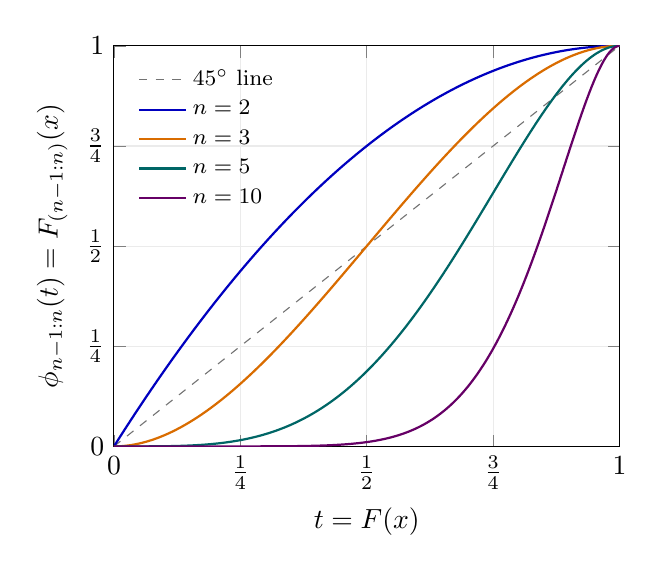
\begin{tikzpicture}
    \begin{axis}[
      width=0.66\textwidth, height=0.55\textwidth,
      xmin=0, xmax=1, ymin=0, ymax=1,
      xlabel={$t = F(x)$},
      ylabel={$\phi_{n-1:n}(t) = F_{(n-1:n)}(x)$},
      xtick={0,0.25,0.5,0.75,1}, ytick={0,0.25,0.5,0.75,1},
      xticklabels={$0$,$\frac{1}{4}$,$\frac{1}{2}$,$\frac{3}{4}$,$1$},
      yticklabels={$0$,$\frac{1}{4}$,$\frac{1}{2}$,$\frac{3}{4}$,$1$},
      grid=major, grid style={black!8},
      legend style={at={(0.03,0.97)}, anchor=north west, font=\footnotesize, draw=none, fill=none},
      legend cell align=left,
      samples=200, domain=0:1,
    ]
      \addplot[black!55, dashed, thin] {x};
      \addlegendentry{$45^\circ$ line}
      \addplot[blue!75!black, thick] {2*x - x^2};
      \addlegendentry{$n = 2$}
      \addplot[orange!85!black, thick] {3*x^2 - 2*x^3};
      \addlegendentry{$n = 3$}
      \addplot[teal!80!black, thick] {5*x^4 - 4*x^5};
      \addlegendentry{$n = 5$}
      \addplot[violet!80!black, thick] {10*x^9 - 9*x^10};
      \addlegendentry{$n = 10$}
    \end{axis}
  \end{tikzpicture}
  \caption{The map $\phi_{n-1:n}(t) = nt^{n-1} - (n-1)t^n$ from the parent CDF to the CDF of the
  second-highest of $n$ draws, for $n = 2, 3, 5, 10$. Each map is a strictly increasing bijection of
  $[0,1]$, so it can be inverted (\cref{prop:B-os-identification}). Every map is flat at $t = 1$, and for $n
  \geq 3$ it is also flat near $t = 0$ over a range that widens with $n$. Where the map is flat, small errors
  in the price distribution become large errors in $F$, so the tails of $F$ are hard to recover from
  transaction prices (\cref{rem:B-os-precision}).}
  \label{fig:B-ordermap}
\end{figure}

\begin{example}[First-price auctions with only the winning bid]\label{ex:B-os-winning-bid}
In a first-price auction with symmetric independent private values, equilibrium bids are i.i.d.\ with some
CDF $G$ and density $g$. A Dutch auction records only the winning bid $B_{(n:n)}$, whose CDF is $G^n$ and
whose density is $nG^{n-1}g$. Hence
\begin{equation*}
  \frac{G_{(n:n)}(b)}{g_{(n:n)}(b)} = \frac{G(b)^n}{nG(b)^{n-1}g(b)} = \frac{G(b)}{n\,g(b)}.
\end{equation*}
The first-order condition of a bidder delivers the inverse bid function of \citet{GuerrePerrigneVuong2000},
which can be rewritten in terms of the winning-bid distribution:
\begin{equation*}
  v = b + \frac{G(b)}{(n-1)g(b)} = b + \frac{n}{n-1}\cdot\frac{G_{(n:n)}(b)}{g_{(n:n)}(b)}.
\end{equation*}
The value distribution is therefore identified from winning bids alone when $n$ is known
\citep[Section~3.3.1, eq.~(3.7)]{AtheyHaile2007}. \Cref{ch:auction-empirics} develops the inversion.
\end{example}

Without symmetry, the parent distributions differ across bidders and one order statistic cannot separate
them. Observing the identity of the winner restores identification. The argument comes from the
statistics of \emph{competing risks}, where a system fails when its first component fails and we observe the
failure time and which component failed \citep{Berman1963}. Up to a sign change, this is the same as
observing the highest bid and the identity of the highest bidder \citep[fn.~21]{AtheyHaile2002}.

\begin{proposition}[Competing risks]\label{prop:B-competing-risks}
Let $X_1, \dots, X_n$ be independent, with continuous CDFs $F_1, \dots, F_n$ that share the support
$[\underline x, \bar x]$. Suppose we observe the maximum $M = \max_i X_i$ and the identity $I$ of the
maximizer. Define $G_i^w(x) = \Pr(M \leq x, I = i)$. Then each $F_i$ is identified, and for every $x$ in the
interior of the support
\begin{equation}\label{eq:B-competing-risks}
  F_i(x) = \exp\left(-\int_x^{\bar x}\frac{\dd G_i^w(t)}{\sum_{j=1}^{n}G_j^w(t)}\right).
\end{equation}
\end{proposition}

\begin{proof}
For transparency we assume densities $f_i$. The general case replaces $f_i(t)\,\dd t$ by $\dd F_i(t)$.

\emph{Step 1.} Bidder $i$ wins with a value at most $x$ when $X_i \leq x$ and every rival draw is below
$X_i$. Conditioning on $X_i = t$ and using independence,
\begin{equation*}
  G_i^w(x) = \Pr\big(X_i \leq x,\ X_j < X_i \ \forall j \neq i\big) = \int_{\underline x}^{x}
  \prod_{j \neq i}F_j(t)\,f_i(t)\,\dd t.
\end{equation*}

\emph{Step 2.} Ties have probability zero, so the events $\{I = j\}$ partition the sample space. Summing over
$j$ gives the CDF of the maximum:
\begin{equation*}
  \sum_{j=1}^{n}G_j^w(x) = \Pr(M \leq x) = \prod_{j=1}^{n}F_j(x) \equiv F_M(x).
\end{equation*}

\emph{Step 3.} For $t$ in the interior of the support, $F_i(t) > 0$. Writing the integrand of Step 1 as
$\frac{F_M(t)}{F_i(t)}f_i(t)$,
\begin{equation*}
  \dd G_i^w(t) = F_M(t)\,\frac{f_i(t)}{F_i(t)}\,\dd t = F_M(t)\,\dd\ln F_i(t).
\end{equation*}

\emph{Step 4.} Divide by $F_M(t)$, which is positive on the interior because the supports coincide, and
integrate from $x$ to $\bar x$:
\begin{equation*}
  \int_x^{\bar x}\frac{\dd G_i^w(t)}{F_M(t)} = \ln F_i(\bar x) - \ln F_i(x) = -\ln F_i(x).
\end{equation*}
Exponentiating and substituting Step 2 for $F_M$ gives \eqref{eq:B-competing-risks}. Every term on the right
is a feature of the distribution of $(M, I)$.
\end{proof}

\Citet[Theorem~2]{AtheyHaile2002} state this result for asymmetric independent private values. Their case
(b) observes the highest bid of a second-price auction together with the winner's identity, which is
\cref{prop:B-competing-risks}. Their case (a) observes the transaction price $X_{(n-1:n)}$ and the winner's
identity, and identification then follows from \citet{Meilijson1981}. We omit that more involved argument.
\citet[Section~3.3.1, eq.~(3.8)]{AtheyHaile2007} apply \eqref{eq:B-competing-risks} to the winning bid and
winner's identity in a first-price auction. This identifies each bidder's bid distribution, and the
first-order conditions then identify the value distributions. The common support matters. If some rival's
values never fall below $a$, bidder $i$ never wins with a value below $a$, so $F_i$ is not identified there.
Theorem~2 relaxes symmetry and keeps independence. Dropping independence as well destroys point
identification, a classic result for competing risks \citep{Tsiatis1975}. \Citet[Theorem~2, p.~2116]{AtheyHaile2002}
also give two routes to testing the model. In the first, participation is exogenous and each bidder faces at
least two different sets of opponents. Each set identifies $F_i$, and the versions must agree. In the second, a
second-price auction reveals both the transaction price and the highest bid, each with the winner's identity.
Cases (a) and (b) then deliver two versions of $F_i$, which again must coincide.

\begin{remark}[Minima and procurement]\label{rem:B-competing-min}
In a procurement auction we observe the lowest cost $m = \min_i X_i$ and the identity of the low bidder. The
mirror image of the proof uses $G_i^\ell(x) = \Pr(m \leq x, I = i) = \int_{\underline x}^{x}\prod_{j \neq
i}[1 - F_j(t)]\,\dd F_i(t)$ and the survival function of the minimum, $S_m(t) = \prod_j[1 - F_j(t)] = 1 -
\sum_jG_j^\ell(t)$. Then $\dd G_i^\ell(t) = -S_m(t)\,\dd\ln[1 - F_i(t)]$, and integrating from $\underline x$
to $x$ gives
\begin{equation*}
  1 - F_i(x) = \exp\left(-\int_{\underline x}^{x}\frac{\dd G_i^\ell(t)}{1 - \sum_{j=1}^{n}G_j^\ell(t)}\right).
\end{equation*}
The integrand is the \emph{cause-specific hazard} of reliability theory.
\end{remark}

\begin{example}[Two exponential suppliers]\label{ex:B-competing-exp}
Let supplier $i \in \{1, 2\}$ have cost $X_i$ with $F_i(x) = 1 - e^{-\lambda_ix}$ on $[0, \infty)$, where the
rates $\lambda_i > 0$ are local notation. The probability that supplier 1 wins at a cost at most $x$ is
\begin{equation*}
  G_1^\ell(x) = \int_0^x e^{-\lambda_2t}\lambda_1e^{-\lambda_1t}\,\dd t
  = \frac{\lambda_1}{\lambda_1 + \lambda_2}\Big(1 - e^{-(\lambda_1 + \lambda_2)x}\Big).
\end{equation*}
The minimum has survival function $S_m(t) = e^{-(\lambda_1 + \lambda_2)t}$. Hence $\frac{\dd
G_1^\ell(t)}{S_m(t)} = \lambda_1\,\dd t$, and the formula of \cref{rem:B-competing-min} returns $1 - F_1(x) =
e^{-\lambda_1x}$. The example shows where the information comes from. The winning cost is exponential with
rate $\lambda_1 + \lambda_2$ whoever wins, and the frequency with which supplier 1 wins, $\frac{\lambda_1}
{\lambda_1 + \lambda_2}$, splits the total rate between the two suppliers.
\end{example}

\subsection{Deconvolution and Kotlarski's lemma}\label{sec:B-kotlarski}

A related tool separates a common component from idiosyncratic ones. It is used for auctions with
unobserved heterogeneity, where all bids in an auction share a component that the econometrician does not
observe. We write $\mathrm{i}$ for the imaginary unit and $\psi_X(t) = \E[e^{\mathrm{i}tX}]$ for the
\emph{characteristic function} of a random variable $X$.

\begin{lemma}[Kotlarski]\label{lem:B-kotlarski}
Let $Y_1, Y_2, Y_3$ be mutually independent with nonvanishing characteristic functions. Assume $\E|Y_1| <
\infty$ and $\E|Y_3| < \infty$, and normalize $\E[Y_1] = 0$. Let $Q_1 = Y_1 + Y_3$ and $Q_2 = Y_2 + Y_3$, with
joint characteristic function $\psi_Q(t_1, t_2) = \E[e^{\mathrm{i}(t_1Q_1 + t_2Q_2)}]$, and let $\partial_1$
denote the derivative with respect to the first argument. Then the distribution of $(Q_1, Q_2)$ determines
the distributions of $Y_1$, $Y_2$ and $Y_3$, through
\begin{equation}\label{eq:B-kotlarski}
  \psi_{Y_3}(t) = \exp\left(\int_0^t\frac{\partial_1\psi_Q(0, u)}{\psi_Q(0, u)}\,\dd u\right), \qquad
  \psi_{Y_1}(t) = \frac{\psi_Q(t, 0)}{\psi_{Y_3}(t)}, \qquad
  \psi_{Y_2}(t) = \frac{\psi_Q(0, t)}{\psi_{Y_3}(t)}.
\end{equation}
\end{lemma}

\begin{proof}
\emph{Step 1 (factorization).} Write $t_1Q_1 + t_2Q_2 = t_1Y_1 + t_2Y_2 + (t_1 + t_2)Y_3$. Independence gives
\begin{equation*}
  \psi_Q(t_1, t_2) = \psi_{Y_1}(t_1)\,\psi_{Y_2}(t_2)\,\psi_{Y_3}(t_1 + t_2).
\end{equation*}

\emph{Step 2 (differentiation).} The moment conditions make $\psi_{Y_1}$ and $\psi_{Y_3}$ differentiable, with
$\psi_{Y_1}'(0) = \mathrm{i}\E[Y_1] = 0$ and $\psi_{Y_1}(0) = 1$. Differentiating Step 1 in $t_1$ at $t_1 = 0$,
\begin{equation*}
  \partial_1\psi_Q(0, u) = \psi_{Y_1}'(0)\psi_{Y_2}(u)\psi_{Y_3}(u) + \psi_{Y_2}(u)\psi_{Y_3}'(u)
  = \psi_{Y_2}(u)\psi_{Y_3}'(u).
\end{equation*}
Since $\psi_Q(0, u) = \psi_{Y_2}(u)\psi_{Y_3}(u)$ and the characteristic functions do not vanish,
\begin{equation*}
  \frac{\partial_1\psi_Q(0, u)}{\psi_Q(0, u)} = \frac{\psi_{Y_3}'(u)}{\psi_{Y_3}(u)}.
\end{equation*}

\emph{Step 3 (integration).} Let $\ell(t) = \int_0^t\frac{\psi_{Y_3}'(u)}{\psi_{Y_3}(u)}\,\dd u$ and $h(t) =
\psi_{Y_3}(t)e^{-\ell(t)}$. Then $h'(t) = \psi_{Y_3}'(t)e^{-\ell(t)} - \psi_{Y_3}(t)\ell'(t)e^{-\ell(t)} = 0$, and
$h(0) = 1$. So $h \equiv 1$, which is the first formula in \eqref{eq:B-kotlarski}. Setting $t_2 = 0$ or $t_1 =
0$ in Step 1 gives the other two. A characteristic function determines its distribution, which completes the
proof.
\end{proof}

The lemma is Lemma~6.1 of \citet{AtheyHaile2007}, after \citet{Kotlarski1966} and \citet{PrakasaRao1992}.
\Cref{lem:15-kotlarski} gives the same result in auction notation, together with identification up to location
when the mean of $Y_1$ is unknown. The normalization is needed because adding a constant to $Y_3$ and subtracting it from $Y_1$ and $Y_2$ leaves
$(Q_1, Q_2)$ unchanged. In auctions with additive unobserved heterogeneity, a bidder's value is
$A_{it} + V_{0t}$, where $V_{0t}$ is common to auction $t$ and unobserved. Equilibrium bids then take the form
$B_{it} = B^0_{it} + V_{0t}$, where the homogenized bid $B^0_{it}$ is the bid in an auction with $V_{0t} = 0$
\citep[Section~6.1.2]{AtheyHaile2007}. Two bids from the same auction play the roles of $Q_1$ and $Q_2$, with
$Y_3 = V_{0t}$. \Cref{lem:B-kotlarski} recovers the distribution of homogenized bids, and the first-order
condition then recovers values. \citet{Krasnokutskaya2011} uses the multiplicative version, which becomes
additive after taking logarithms (\cref{ch:auction-empirics}).

\section{Fixed points and the contraction mapping theorem}\label{sec:B-fixedpoint}

Many objects in industrial organization are \emph{fixed points}, points $x^*$ with $\Phi(x^*) = x^*$ for some
map $\Phi$. The mean utilities that rationalize observed shares solve $\delta = \delta + \ln s^{obs} - \ln
s(\delta)$. Equilibrium prices solve $p = BR(p)$, where $BR$ stacks the firms' best responses. Value
functions of dynamic problems solve Bellman equations. Each case raises three questions. Does a fixed point
exist? Is it unique? How do we compute it? The contraction mapping theorem answers all three at once when it
applies. Brouwer's and Kakutani's theorems answer only the first, and uniqueness then needs a separate
argument such as diagonal dominance. The proof of the implicit function theorem (\cref{thm:B-ift}) already
relied on the contraction mapping theorem, which we now prove. Throughout, $\Phi$ is the map, $\kappa \in [0,1)$
a modulus, $x^*$ a fixed point and $x^{(h)}$ the $h$-th iterate.

\subsection{Metric spaces and contractions}\label{sec:B-metric}

\begin{definition}[Metric space]\label{def:B-metric}
A \emph{metric space} is a set $X$ with a function $d: X \times X \to [0, \infty)$ with three properties
for all $x, y, z \in X$.
\begin{enumerate}[label=(\roman*)]
  \item $d(x, y) = 0$ if and only if $x = y$.
  \item $d(x, y) = d(y, x)$.
  \item $d(x, z) \leq d(x, y) + d(y, z)$.
\end{enumerate}
A sequence $(x^{(h)})$ is \emph{Cauchy} if for every $\epsilon > 0$ there is $H$ with $d(x^{(h)},
x^{(m)}) < \epsilon$ for all $h, m \geq H$. The space is \emph{complete} if every Cauchy sequence converges
to a point of $X$.
\end{definition}

The leading example is $\R^n$ with the sup norm $\|x\|_\infty = \max_k |x_k|$ and $d(x, y) = \|x -
y\|_\infty$. A sequence that is Cauchy in this metric is Cauchy coordinate by coordinate, and $\R$ is
complete, so $(\R^n, \|\cdot\|_\infty)$ is complete. A closed subset of a complete space is complete, because
limits of its sequences stay in the set. Boxes $[\underline y, \bar y]^J$ and orthants $(-\infty, \bar
\delta]^J$ are therefore complete. The interval $(0, 1]$ is not complete, since the Cauchy sequence
$\frac{1}{h}$ converges to $0 \notin (0,1]$. The set of bounded real functions on a set $S$, with the metric
$\sup_{s \in S}|g(s) - g'(s)|$, is complete. So is its subset of bounded continuous functions when $S$ is a
metric space \citep{StokeyLucas1989}. Dynamic programming works in these function spaces.

\begin{definition}[Contraction]\label{def:B-contraction}
A map $\Phi: X \to X$ is a \emph{contraction with modulus} $\kappa \in [0,1)$ if
\begin{equation*}
  d\big(\Phi(x), \Phi(y)\big) \leq \kappa\, d(x, y) \qquad \text{for all } x, y \in X.
\end{equation*}
\end{definition}

A map that satisfies the inequality with some $\kappa \geq 0$ is \emph{Lipschitz} with constant $\kappa$. A
contraction is Lipschitz and hence continuous. The uniform modulus is essential. Consider $\Phi(x) = x +
\frac{1}{x}$ on $[1, \infty)$. It maps the set into $[2, \infty)$, and $\Phi'(x) = 1 - \frac{1}{x^2} \in [0,
1)$, so the mean value theorem gives $|\Phi(x) - \Phi(y)| < |x - y|$ whenever $x \neq y$. Yet $\Phi(x) = x$
would require $\frac{1}{x} = 0$, so there is no fixed point. The local modulus $\Phi'(x)$ approaches one as $x
\to \infty$, and the iterates drift off to infinity. The share inversion has the same feature, which is why
\citet{BerryLevinsohnPakes1995} truncate the map (\cref{thm:B-blp-contraction}). Completeness matters too.
The map $\Phi(x) = \frac{x}{2}$ is a contraction of $(0,1]$ into itself without a fixed point in $(0,1]$.

\subsection{The Banach fixed-point theorem}\label{sec:B-banach}

\begin{theorem}[Banach fixed-point theorem]\label{thm:B-banach}
Let $(X, d)$ be a complete metric space and let $\Phi: X \to X$ be a contraction with modulus $\kappa$. Then
the following hold.
\begin{enumerate}[label=(\roman*)]
  \item $\Phi$ has exactly one fixed point $x^*$.
  \item For every starting point $x^{(0)} \in X$, the iterates $x^{(h+1)} = \Phi(x^{(h)})$ converge to $x^*$.
  \item $d(x^{(h)}, x^*) \leq \kappa^h\,d(x^{(0)}, x^*)$ for all $h$.
\end{enumerate}
\end{theorem}

\begin{proof}
\emph{Step 1 (successive steps shrink geometrically).} For $h \geq 1$,
\begin{equation*}
  d\big(x^{(h+1)}, x^{(h)}\big) = d\big(\Phi(x^{(h)}), \Phi(x^{(h-1)})\big) \leq \kappa\,d\big(x^{(h)},
  x^{(h-1)}\big).
\end{equation*}
Applying this $h$ times gives $d(x^{(h+1)}, x^{(h)}) \leq \kappa^h d_0$, where $d_0 = d(x^{(1)}, x^{(0)})$.

\emph{Step 2 (the iterates form a Cauchy sequence).} For $m > h$, the triangle inequality and Step 1 give
\begin{equation*}
  d\big(x^{(m)}, x^{(h)}\big) \leq \sum_{l=h}^{m-1}d\big(x^{(l+1)}, x^{(l)}\big) \leq d_0\sum_{l=h}^{m-1}
  \kappa^l \leq \frac{\kappa^h}{1 - \kappa}\,d_0.
\end{equation*}
The bound tends to zero as $h \to \infty$, so the sequence is Cauchy. By completeness it converges to some
$x^* \in X$.

\emph{Step 3 (the limit is a fixed point).} For every $h$,
\begin{equation*}
  d\big(\Phi(x^*), x^*\big) \leq d\big(\Phi(x^*), \Phi(x^{(h)})\big) + d\big(x^{(h+1)}, x^*\big)
  \leq \kappa\,d\big(x^*, x^{(h)}\big) + d\big(x^{(h+1)}, x^*\big).
\end{equation*}
The right side tends to zero, so $\Phi(x^*) = x^*$.

\emph{Step 4 (uniqueness).} If $\Phi(y) = y$, then $d(x^*, y) = d(\Phi(x^*), \Phi(y)) \leq \kappa\,d(x^*, y)$.
Since $\kappa < 1$, this forces $d(x^*, y) = 0$.

\emph{Step 5 (the rate).} $d(x^{(h)}, x^*) = d(\Phi(x^{(h-1)}), \Phi(x^*)) \leq \kappa\,d(x^{(h-1)}, x^*)$, and
induction gives (iii).
\end{proof}

The theorem is due to \citet{Banach1922}. Part (iii) says that the error falls at least geometrically, a
property called \emph{linear convergence}. In practice we do not know $x^*$, so we need bounds in terms of
computable quantities.

\begin{corollary}[Error bounds]\label{cor:B-banach-bounds}
Under the conditions of \cref{thm:B-banach}, for every $h \geq 1$,
\begin{align}
  d\big(x^{(h)}, x^*\big) &\leq \frac{\kappa^h}{1 - \kappa}\,d\big(x^{(1)}, x^{(0)}\big)
  && \text{(a priori bound)}, \label{eq:B-apriori}\\
  d\big(x^{(h)}, x^*\big) &\leq \frac{\kappa}{1 - \kappa}\,d\big(x^{(h)}, x^{(h-1)}\big)
  && \text{(a posteriori bound)}. \label{eq:B-aposteriori}
\end{align}
\end{corollary}

\begin{proof}
For \eqref{eq:B-apriori}, let $m \to \infty$ in Step 2 of the proof of \cref{thm:B-banach}, using continuity
of $d$. For \eqref{eq:B-aposteriori}, apply the triangle inequality and the contraction property:
\begin{align*}
  d\big(x^{(h)}, x^*\big) &= d\big(\Phi(x^{(h-1)}), \Phi(x^*)\big) \leq \kappa\,d\big(x^{(h-1)}, x^*\big) \\
  &\leq \kappa\,d\big(x^{(h-1)}, x^{(h)}\big) + \kappa\,d\big(x^{(h)}, x^*\big).
\end{align*}
Collecting the terms in $d(x^{(h)}, x^*)$ gives $(1 - \kappa)\,d(x^{(h)}, x^*) \leq \kappa\,d(x^{(h)},
x^{(h-1)})$.
\end{proof}

The a posteriori bound justifies the usual stopping rule, which halts when successive iterates are within
a tolerance $\varepsilon_{tol}$. The rule controls the true error only up to the factor $\frac{\kappa}{1 -
\kappa}$. This factor is 1 for $\kappa = \frac{1}{2}$, 9 for $\kappa = 0.9$ and 99 for $\kappa = 0.99$, so the
stopping tolerance must be tighter than the accuracy we want when $\kappa$ is near one.
\Cref{prop:08-innererror} applies this bound to the inner loop of BLP estimation. The a priori bound tells us
how many iterations suffice. The bound is below $\varepsilon_{tol}$ when $\kappa^h d(x^{(1)}, x^{(0)}) \leq
\varepsilon_{tol}(1 - \kappa)$. Taking logarithms and dividing by $\ln\kappa < 0$, which reverses the
inequality,
\begin{equation}\label{eq:B-iterations}
  h \geq \frac{\ln\big(\varepsilon_{tol}(1 - \kappa)\big) - \ln d\big(x^{(1)}, x^{(0)}\big)}{\ln\kappa}.
\end{equation}
With $d(x^{(1)}, x^{(0)}) = 1$ and $\varepsilon_{tol} = 10^{-12}$, the bound requires 41 iterations for $\kappa =
\frac{1}{2}$, 285 for $\kappa = 0.9$ and 3,208 for $\kappa = 0.99$. The cost of a fixed-point computation grows
roughly like $\frac{1}{1 - \kappa}$.

\begin{remark}[Contractions on subsets]\label{rem:B-local-contraction}
The theorem applies to any closed subset $C \subseteq X$ that $\Phi$ maps into itself and on which $\Phi$
contracts, since $C$ is complete. A convenient sufficient condition uses a closed ball. Suppose $\Phi$ is
Lipschitz with constant $\kappa < 1$ on $\bar B = \{x : d(x, x^{(0)}) \leq \tau\}$ and $d(\Phi(x^{(0)}),
x^{(0)}) \leq (1 - \kappa)\tau$. Then for $x \in \bar B$,
\begin{equation*}
  d\big(\Phi(x), x^{(0)}\big) \leq d\big(\Phi(x), \Phi(x^{(0)})\big) + d\big(\Phi(x^{(0)}), x^{(0)}\big)
  \leq \kappa\tau + (1 - \kappa)\tau = \tau,
\end{equation*}
so $\Phi$ maps $\bar B$ into itself and has a unique fixed point there. The proof of the implicit function
theorem (\cref{thm:B-ift}) uses this device, and so does the truncation argument of
\cref{thm:B-blp-contraction}.
\end{remark}

\begin{remark}[Local convergence and the choice of norm]\label{rem:B-ostrowski}
Suppose $\Phi: \R^n \to \R^n$ is continuously differentiable near a fixed point $x^*$. If the spectral radius
of the Jacobian $D\Phi(x^*)$, the largest modulus of its eigenvalues, is below one, then the iterates
converge to $x^*$ from every starting point close enough to it. The asymptotic rate equals the spectral
radius. If some eigenvalue has modulus above one, $x^*$ repels the iterates in the direction of the
corresponding eigenvector, and iteration started near $x^*$ generally fails to converge \citep{Judd1998}.
The contraction property depends on the metric. The matrix $A = \begin{psmallmatrix}0 & 2\\ 0 &
0\end{psmallmatrix}$ has spectral radius zero, and $A^2x = 0$ for every $x$, yet $\|Ax\|_\infty = 2\|x\|_\infty$
for $x = (0, 1)$. The sup norm suits the applications below because row sums of Jacobians are easy to bound.
\end{remark}

\Cref{fig:B-cobweb} shows the iteration on the real line as a \emph{cobweb}. Each step moves vertically to
the graph of $\Phi$ and then horizontally to the 45-degree line. In the left panel, $\Phi(x) = 1 +
\frac{1}{2}\cos x$ has $|\Phi'(x)| = \frac{1}{2}|\sin x| \leq \frac{1}{2}$, so it is a contraction of $\R$ with
modulus $\frac{1}{2}$. Starting from $x^{(0)} = 0$, the iterates are $1.5$, $1.035$, $1.255$, $1.155$ and so on,
and they converge to $x^* = 1.187151$. After ten steps the error is $3.2 \times 10^{-4}$, below the a priori
bound $\frac{\kappa^{10}}{1 - \kappa}\,d(x^{(1)}, x^{(0)}) = 2^{-9} \times 1.5 = 2.9 \times 10^{-3}$. The errors shrink by a factor close to
$|\Phi'(x^*)| = 0.464$ per step, as \cref{rem:B-ostrowski} predicts. In the right panel, $\Phi(x) = 3 -
\frac{3}{2}x$ has slope $-\frac{3}{2}$. Its fixed point is $x^* = \frac{6}{5}$, but from $x^{(0)} = 1$ the
distance to $x^*$ grows by the factor $\frac{3}{2}$ each step, from $0.2$ to $0.3$, $0.45$, $0.675$ and
beyond. The negative slope makes the path spiral, and the slope above one in absolute value makes it diverge.

\begin{figure}[htbp]
  \centering
  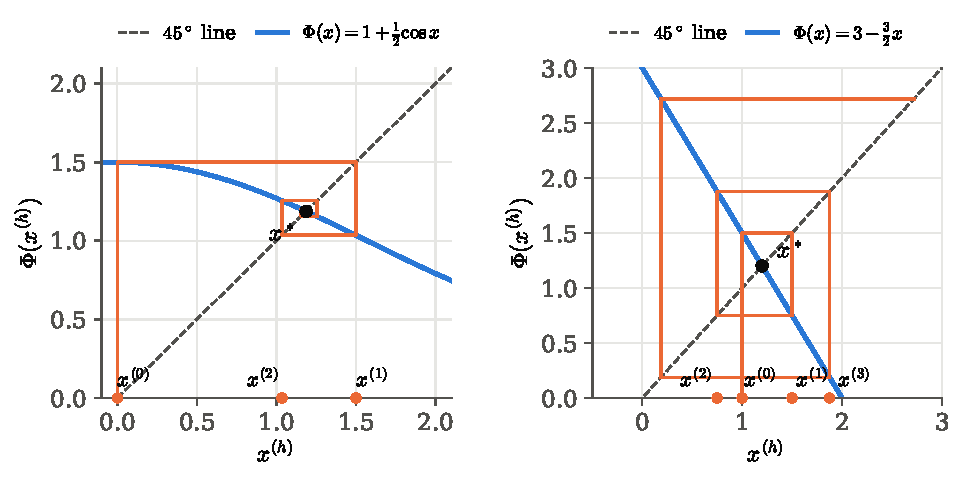
\includegraphics[width=0.95\textwidth]{figures/appB/cobweb.pdf}
  \caption{Cobweb diagrams for the iteration $x^{(h+1)} = \Phi(x^{(h)})$. In the left panel, $\Phi(x) = 1 +
  \frac{1}{2}\cos x$ is a contraction with modulus $\frac{1}{2}$, and the path from $x^{(0)} = 0$ converges to
  the fixed point $x^* \approx 1.187$. In the right panel, $\Phi(x) = 3 - \frac{3}{2}x$ has slope $-\frac{3}{2}$, and the path
  from $x^{(0)} = 1$ spirals away from the fixed point $x^* = \frac{6}{5}$.}
  \label{fig:B-cobweb}
\end{figure}

\subsection{Checking the contraction property}\label{sec:B-contraction-criteria}

For smooth maps on $\R^n$, the contraction property follows from a bound on the Jacobian.

\begin{proposition}[Jacobian row-sum criterion]\label{prop:B-jacobian-criterion}
Let $X \subseteq \R^n$ be convex and let $\Phi: X \to \R^n$ be continuously differentiable on an open set
containing $X$. If
\begin{equation}\label{eq:B-rowsum-criterion}
  \sup_{x \in X}\ \max_{j}\sum_{k=1}^{n}\left|\frac{\partial\Phi_j(x)}{\partial x_k}\right| \leq \kappa,
\end{equation}
then $\|\Phi(x) - \Phi(y)\|_\infty \leq \kappa\|x - y\|_\infty$ for all $x, y \in X$. If in addition $\kappa < 1$
and $\Phi$ maps $X$ into itself, then $\Phi$ is a contraction of $X$ in the sup norm.
\end{proposition}

\begin{proof}
Fix $x, y \in X$ and a component $j$. By convexity the segment $x + \tau(y - x)$, $\tau \in [0,1]$, lies in
$X$. The fundamental theorem of calculus and the chain rule give
\begin{equation*}
  \Phi_j(y) - \Phi_j(x) = \int_0^1\sum_{k=1}^{n}\frac{\partial\Phi_j}{\partial x_k}\big(x + \tau(y -
  x)\big)\,(y_k - x_k)\,\dd\tau.
\end{equation*}
Bounding each $|y_k - x_k|$ by $\|y - x\|_\infty$,
\begin{equation*}
  |\Phi_j(y) - \Phi_j(x)| \leq \int_0^1\sum_{k=1}^{n}\left|\frac{\partial\Phi_j}{\partial x_k}\big(x +
  \tau(y - x)\big)\right|\,\dd\tau\ \|y - x\|_\infty \leq \kappa\|y - x\|_\infty.
\end{equation*}
Taking the maximum over $j$ proves the claim.
\end{proof}

The constant in \eqref{eq:B-rowsum-criterion} is the largest induced sup norm of the Jacobian over $X$, by
\cref{lem:B-rowsum}. For a linear map the criterion is therefore sharp. The proof is the mean value
inequality of \cref{sec:B-calculus}.

When all partial derivatives are nonnegative, as in the share inversion below, the absolute values in
\eqref{eq:B-rowsum-criterion} drop out. The row sum then has a direct reading:
\begin{equation*}
  \sum_{k=1}^{n}\frac{\partial\Phi_j(x)}{\partial x_k} = \frac{\dd}{\dd c}\,\Phi_j(x + c\mathbf{1})\Big|_{c=0},
\end{equation*}
where $\mathbf{1}$ is the vector of ones. The condition says that $\Phi$ is monotone and that raising every
argument by $c$ raises each component by less than $c$. Blackwell's theorem is the version of this idea for
maps between function spaces.

\begin{theorem}[\citealp{Blackwell1965}]\label{thm:B-blackwell}
Let $B(S)$ be the space of bounded real functions on a set $S$ with the sup metric, and let $\mathcal{T}:
B(S) \to B(S)$ satisfy two conditions. The first, monotonicity, requires that $g \leq g'$ pointwise implies
$\mathcal{T}g \leq \mathcal{T}g'$. The second, discounting, requires that there is $\kappa \in [0,1)$ such that $\mathcal{T}(g + c) \leq \mathcal{T}g +
\kappa c$ for every $g$ and every constant $c \geq 0$. Then $\mathcal{T}$ is a contraction with modulus $\kappa$.
\end{theorem}

\begin{proof}
Fix $g, g' \in B(S)$ and let $c = \sup_s|g(s) - g'(s)|$. Then $g \leq g' + c$ pointwise. Monotonicity and
discounting give $\mathcal{T}g \leq \mathcal{T}(g' + c) \leq \mathcal{T}g' + \kappa c$. Exchanging the roles
of $g$ and $g'$ gives $\mathcal{T}g' \leq \mathcal{T}g + \kappa c$. Hence $|\mathcal{T}g(s) - \mathcal{T}g'(s)|
\leq \kappa c$ for every $s$, which is the claim.
\end{proof}

The Bellman operator $(\mathcal{T}g)(s) = \max_a\{u(s, a) + \kappa\,\E[g(s') \mid s, a]\}$ of a dynamic program
with discount factor $\kappa$ satisfies both conditions, so value functions are unique fixed points that
value iteration computes. Dynamic models lie outside this edition, but the logic is the same as in the
static applications below.

Some maps of interest have row sums below one at every point but not uniformly, as in the example $x +
\frac{1}{x}$. \Citet[Appendix~I]{BerryLevinsohnPakes1995} handle this case with a truncation.

\begin{theorem}[\citealp{BerryLevinsohnPakes1995}, Appendix I]\label{thm:B-blp-contraction}
Consider $\R^J$ with the sup norm, and let $\Phi: \R^J \to \R^J$ satisfy three conditions. (1) $\Phi$ is
continuously differentiable, with $\frac{\partial\Phi_j(y)}{\partial y_k} \geq 0$ and $\sum_{k=1}^{J}
\frac{\partial\Phi_j(y)}{\partial y_k} < 1$ for all $j$, $k$ and $y$. (2) $\Phi$ is bounded below:
$\underline y \equiv \min_j\inf_y\Phi_j(y) > -\infty$. (3) There is a value $\bar y$ such that, whenever $y_j
\geq \bar y$ for some $j$, there is some $k$ (not necessarily equal to $j$) with $\Phi_k(y) < y_k$. Then
$\Phi$ has a unique fixed point in $\R^J$. Moreover, the truncated map $\hat\Phi_j(y) = \min\{\Phi_j(y),
\bar y\}$ is a contraction of $[\underline y, \bar y]^J$ with modulus below one.
\end{theorem}

\Cref{thm:08-contraction} proves the theorem in full. The idea is short. On the compact set $[\underline y,
\bar y]^J$, enlarged by the segments along which the proof integrates, the continuous row sums attain a
maximum $\kappa < 1$. The truncated map is therefore a contraction there, and \cref{thm:B-banach} gives a
fixed point. Condition (3) keeps that fixed point away from the cap $\bar y$, so it is a fixed point of
$\Phi$ itself. The bound $\bar y$ is needed because no uniform modulus exists on all of $\R^J$. In the logit
model, for instance, the row sums of the share-inversion map equal $1 - s_0(\delta)$, which tends to one as
the mean utilities grow (\cref{sec:B-inversion}).

\subsection{Application: inverting market shares}\label{sec:B-inversion}

Consider a market with inside goods $j = 1, \dots, J$ and the outside good $j = 0$. In the random
coefficients logit model, consumer $i$ chooses $j$ with probability
\begin{equation*}
  s_{ij}(\delta) = \frac{e^{\delta_j + \mu_{ij}}}{1 + \sum_{k=1}^{J}e^{\delta_k + \mu_{ik}}}, \qquad
  s_{i0}(\delta) = 1 - \sum_{k=1}^{J}s_{ik}(\delta),
\end{equation*}
and the market share is $s_j(\delta) = \int s_{ij}(\delta)\,\dd F(\nu_i)$, where $\mu_{ij}$ depends on the
consumer's tastes $\nu_i$ and the nonlinear parameters (\cref{ch:blp}). Given observed shares $s^{obs}$
with $s^{obs}_j > 0$ and $\sum_js^{obs}_j < 1$, estimation needs the vector $\delta$ that solves $s(\delta) =
s^{obs}$. \citet[eq.~(6.8), p.~865]{BerryLevinsohnPakes1995} compute it as the fixed point of
\begin{equation}\label{eq:B-blp-map}
  \Phi_j(\delta) = \delta_j + \ln s^{obs}_j - \ln s_j(\delta), \qquad j = 1, \dots, J.
\end{equation}
A vector $\delta$ is a fixed point of $\Phi$ exactly when $s(\delta) = s^{obs}$.

\begin{proposition}[Row sums of the BLP map]\label{prop:B-blp-rowsum}
In the random coefficients logit model, for all $j$ and all $k \neq j$,
\begin{equation*}
  \frac{\partial\Phi_j}{\partial\delta_j} = \frac{1}{s_j}\int s_{ij}^2\,\dd F > 0, \qquad
  \frac{\partial\Phi_j}{\partial\delta_k} = \frac{1}{s_j}\int s_{ij}s_{ik}\,\dd F > 0,
\end{equation*}
and the row sums are
\begin{equation}\label{eq:B-blp-rowsum}
  \sum_{k=1}^{J}\frac{\partial\Phi_j}{\partial\delta_k} = 1 - \frac{1}{s_j}\int s_{ij}s_{i0}\,\dd F \in (0, 1).
\end{equation}
\end{proposition}

\begin{proof}
The individual logit derivatives are $\frac{\partial s_{ij}}{\partial\delta_k} = s_{ij}(\indic\{j = k\} -
s_{ik})$, bounded by one, so we may differentiate under the integral (\cref{sec:B-calculus}). Hence
$\frac{\partial s_j}{\partial\delta_j} = \int s_{ij}(1 - s_{ij})\,\dd F$ and $\frac{\partial
s_j}{\partial\delta_k} = -\int s_{ij}s_{ik}\,\dd F$ for $k \neq j$. Differentiating \eqref{eq:B-blp-map},
\begin{equation*}
  \frac{\partial\Phi_j}{\partial\delta_j} = 1 - \frac{1}{s_j}\int s_{ij}(1 - s_{ij})\,\dd F
  = 1 - \frac{s_j}{s_j} + \frac{1}{s_j}\int s_{ij}^2\,\dd F = \frac{1}{s_j}\int s_{ij}^2\,\dd F,
\end{equation*}
and $\frac{\partial\Phi_j}{\partial\delta_k} = -\frac{1}{s_j}\frac{\partial s_j}{\partial\delta_k} =
\frac{1}{s_j}\int s_{ij}s_{ik}\,\dd F$. For the row sum, consumer $i$'s choice probabilities depend only on
differences of the utilities $(\delta_0 + \mu_{i0}, \dots, \delta_J + \mu_{iJ})$, with $\delta_0 = \mu_{i0} = 0$.
By \cref{cor:B-translation}, $\sum_{k=0}^{J}\frac{\partial s_{ij}}{\partial\delta_k} = 0$, and the outside
derivative is $\frac{\partial s_{ij}}{\partial\delta_0} = -s_{ij}s_{i0}$. Hence $\sum_{k=1}^{J}\frac{\partial
s_{ij}}{\partial\delta_k} = s_{ij}s_{i0}$. Integrating and dividing by $s_j$,
\begin{equation*}
  \sum_{k=1}^{J}\frac{\partial\Phi_j}{\partial\delta_k} = 1 - \frac{1}{s_j}\sum_{k=1}^{J}\frac{\partial
  s_j}{\partial\delta_k} = 1 - \frac{1}{s_j}\int s_{ij}s_{i0}\,\dd F.
\end{equation*}
The integral is positive and smaller than $\int s_{ij}\,\dd F = s_j$, so the row sum lies in $(0,1)$.
\end{proof}

\Cref{cor:08-rowsum} gives the same computation, and \cref{ch:blp} verifies the remaining conditions of
\cref{thm:B-blp-contraction}. The row sum has a useful reading. The weights $\frac{s_{ij}}{s_j}$ form the
distribution of consumer types among the buyers of $j$. The row sum is therefore one minus the average
probability of choosing the outside good among those buyers. The modulus is close to one when the buyers of
some product rarely choose the outside good, and convergence is then slow. The plain logit model shows this in
its simplest form. There $s_{ij} = s_j$, so $\frac{\partial\Phi_j}{\partial\delta_k} = s_k$ for every $k$,
including $k = j$. The Jacobian is the rank-one matrix $\mathbf{1}s^\T$, whose only nonzero eigenvalue is
$s^\T\mathbf{1} = 1 - s_0$. With $s_0 = 0.1$ the iteration gains one digit of accuracy only every 22 steps,
since $\frac{\ln 10}{-\ln 0.9} \approx 21.9$, although the logit inverse $\delta_j = \ln s_j - \ln s_0$ is
available in closed form.

Three practical rules follow. First, the logit inversion $\ln s^{obs}_j - \ln s^{obs}_0$ is a natural
starting value, and inside an estimation routine the solution at the previous parameter value is better.
Second, the stopping tolerance must be tight, by \eqref{eq:B-aposteriori}, because the inversion error
propagates into the estimation objective (\cref{prop:08-innererror}). \citet{DubeFoxSu2012} study how to improve
the numerical performance of random coefficients demand estimation (\cref{ch:blp}).
Third, the update can be written
multiplicatively as $e^{\delta^{(h+1)}_j} = e^{\delta^{(h)}_j}\frac{s^{obs}_j}{s_j(\delta^{(h)})}$. Each step
raises $\delta_j$ when the model underpredicts the share of $j$ and lowers it when the model overpredicts.

\begin{remark}[Where the iteration typically moves from the logit start]\label{rem:B-logit-start}
For a product with a small share, the logistic function $\frac{e^{u}}{1 + e^{u}}$ is convex in the relevant
range of utilities. Random coefficients spread individual utilities around $\delta_j$. By Jensen's
inequality the average choice probability at a given $\delta$ then exceeds the logit probability, so the
model share at the logit starting value typically exceeds the observed share. The iteration then lowers
$\delta_j$, and the recovered mean utilities typically lie below the logit start. The statement describes a
tendency. It is not a theorem, because the denominators of all products move together. \Cref{ch:blp} and \cref{app:problems}
report worked examples.
\end{remark}

\citet[Appendix]{Berry1994} proved existence and uniqueness of the inverse for a broad class of discrete
choice models without the contraction. His argument combines Brouwer's theorem with a diagonal dominance
condition.

\begin{proposition}[\citealp{Berry1994}, Appendix]\label{prop:B-berry-inverse}
Let $s: \R^J \to (0,1)^J$ be the inside shares of a random utility model with $\delta_0 = 0$. Suppose $s$ is
continuously differentiable, and that for all goods $j, k \in \{0, 1, \dots, J\}$ the share of $j$ rises in
$\delta_j$ and falls in $\delta_k$ for $k \neq j$. Suppose also that, for any values of the other inside mean
utilities, finite or $-\infty$, $s_j \to 0$ as $\delta_j \to -\infty$ and $s_j \to 1$ as $\delta_j \to \infty$. Then for every $s^{obs}$ with positive entries and $\sum_j
s^{obs}_j < 1$ there is exactly one $\delta$ with $s(\delta) = s^{obs}$.
\end{proposition}

\begin{proof}[Outline of the proof]
\emph{Step 1 (the element-by-element inverse).} For each $j$, let $r_j(\delta)$ be the value of $\delta_j$
that makes $s_j(\delta_1, \dots, r_j, \dots, \delta_J) = s^{obs}_j$, given the other mean utilities. It exists,
is unique and is continuous, by monotonicity and the limits. It does not depend on $\delta_j$. The implicit
function theorem (\cref{thm:B-ift}) gives, for $k \neq j$,
\begin{equation*}
  \frac{\partial r_j}{\partial\delta_k} = -\left(\frac{\partial s_j}{\partial\delta_j}\right)^{-1}
  \frac{\partial s_j}{\partial\delta_k} > 0.
\end{equation*}
A vector $\delta$ solves $s(\delta) = s^{obs}$ if and only if it is a fixed point of $r = (r_1, \dots, r_J)$.

\emph{Step 2 (a lower bound).} Since $r_j$ rises in every $\delta_k$, it is bounded below by its limit as all
other $\delta_k \to -\infty$. Let $\underline\delta$ be the smallest of these $J$ limits.

\emph{Step 3 (an upper bound).} For each $j$, let $\bar\delta_j$ be the value of $\delta_j$ that sets the
outside share equal to $s^{obs}_0 = 1 - \sum_ks^{obs}_k$ when all other inside $\delta_k$ are $-\infty$. Choose
$\bar\delta > \max_j\bar\delta_j$. Suppose $\delta_j \geq \bar\delta$ for some $j$. Adding products and
raising $\delta_j$ both lower the outside share, so $s_0(\delta) < s^{obs}_0$. The inside shares then sum to
more than $\sum_ks^{obs}_k$, so $s_k(\delta) > s^{obs}_k$ for some $k$. For that $k$, matching the smaller
observed share requires a lower utility, so $r_k(\delta) < \delta_k$.

\emph{Step 4 (existence).} The truncated map $\bar r_j(\delta) = \min\{r_j(\delta), \bar\delta\}$ is continuous
and maps the box $[\underline\delta, \bar\delta]^J$ into itself. Brouwer's theorem (\cref{thm:B-brouwer})
gives a fixed point $\delta^*$. If $\delta^*_j = \bar\delta$ for some $j$, Step 3 gives $k$ with $\bar
r_k(\delta^*) \leq r_k(\delta^*) < \delta^*_k$, a contradiction. So $\delta^*$ lies below the cap and is a fixed
point of $r$.

\emph{Step 5 (uniqueness).} Shares depend only on utility differences, so \cref{cor:B-translation} gives
$\sum_{k=0}^{J}\frac{\partial s_j}{\partial\delta_k} = 0$. All cross derivatives are negative, including the
one with respect to $\delta_0$. Hence
\begin{equation}\label{eq:B-berry-dd}
  \frac{\partial s_j}{\partial\delta_j} = \sum_{k \neq j,\ k \geq 1}\left|\frac{\partial
  s_j}{\partial\delta_k}\right| + \left|\frac{\partial s_j}{\partial\delta_0}\right| > \sum_{k \neq j,\ k \geq
  1}\left|\frac{\partial s_j}{\partial\delta_k}\right|.
\end{equation}
Dividing by $\frac{\partial s_j}{\partial\delta_j}$ shows that the row sums $\sum_k\big|\frac{\partial
r_j}{\partial\delta_k}\big|$ are below one at every point. On the compact box their maximum $\kappa$ is
below one. The truncation is nonexpansive, so \cref{prop:B-jacobian-criterion} makes $\bar r$ a contraction
of the box. Every solution lies in the box by Steps 2 and 3, so the solution is unique.
\end{proof}

Condition \eqref{eq:B-berry-dd} is (A2) in \citet[p.~261]{Berry1994}. It also makes the Jacobian
$\frac{\partial s}{\partial\delta^\T}$ strictly diagonally dominant, hence nonsingular by \cref{lem:B-dd}.
\Citet[p.~260]{Berry1994} notes that a strictly positive and continuous density of the consumer-level
unobservables suffices for his sign conditions. On the same page he states the limit conditions for finite
values of the other mean utilities. We also allow the value $-\infty$, which Steps 2 and 3 of the proof use.

\begin{remark}[Connected substitutes]\label{rem:B-connected-substitutes}
\citet{BerryGandhiHaile2013} replace Berry's sign conditions by a weaker structure. Write $s_j(\delta, p)$
for the demand system and let $\lambda$ stand for either $-p$ or $\delta$. Goods $0, 1, \dots, J$ are
\emph{connected substitutes} in $\lambda$ if two conditions hold \citep[Definition~1,
p.~1759]{BerryHaile2014}. First, $s_k$ is nonincreasing in $\lambda_j$ for all $j > 0$ and $k \neq j$. Second,
for every nonempty set $\mathcal{K} \subseteq \{1, \dots, J\}$, some $k \in \mathcal{K}$ and some good $\ell
\notin \mathcal{K}$ have $s_\ell$ strictly decreasing in $\lambda_k$. The first condition requires weak gross
substitutes. The second requires enough strict substitution that no group of inside goods trades only among
itself, where the outside good may serve as the good $\ell$. Connected substitutes are combined with an
\emph{index restriction}. One observed characteristic $x^{(1)}_{jt}$ and the unobservable $\xi_{jt}$ affect the
distribution of utilities only through the scalar index $\delta_{jt} = x^{(1)}_{jt}\beta_j + \xi_{jt}$, so
consumers treat them as perfect substitutes \citep[Section~3.2, eq.~(2) and Assumption~1, p.~1757]{BerryHaile2014}.
Under the index restriction and connected substitutes in both $-p$ and $\delta$, there is at most one $\delta$
with $s(\delta, p) = s^{obs}$ for any interior share vector. This is Lemma~1 of \citet[p.~1760]{BerryHaile2014},
who credit the proof to \citet{BerryGandhiHaile2013}. The result needs no functional form, and it allows zero
cross effects, as in the vertical model where each product competes only with its neighbors (\cref{ch:discrete}).
It delivers injectivity. Existence must be argued separately.
\end{remark}

Nested logit demand shows why the BLP map sometimes needs to be modified. With nests $g$, nesting parameter
$\sigma \in [0, 1)$ and within-nest shares $s_{j|g}$, the derivatives of the log shares are given by
\eqref{eq:B-nl-logderiv} in \cref{prop:B-nested-inversion}. The own derivative
$\frac{\partial\ln s_j}{\partial\delta_j} = \frac{1}{1-\sigma} - \frac{\sigma}{1-\sigma}s_{j|g} - s_j$ can be far above one when
$\sigma$ is large. The diagonal partial of the BLP map, $1 -
\frac{\partial\ln s_j}{\partial\delta_j}$, is then negative, and the map can fail to be a contraction.

\begin{proposition}[Dampened inversion for the nested logit]\label{prop:B-nl-dampening}
Consider the nested logit model and the dampened map
\begin{equation}\label{eq:B-nl-dampened}
  \Phi^D(\delta) = \delta + (1 - \sigma)\big[\ln s^{obs} - \ln s(\delta)\big].
\end{equation}
(i) For $j$ in nest $g$, its partial derivatives are all nonnegative:
\begin{equation*}
  \frac{\partial\Phi^D_j}{\partial\delta_k} =
  \begin{cases}
    \sigma s_{j|g} + (1 - \sigma)s_j, & k = j,\\[2pt]
    \sigma s_{k|g} + (1 - \sigma)s_k, & k \neq j,\ k \in g,\\[2pt]
    (1 - \sigma)s_k, & k \notin g.
  \end{cases}
\end{equation*} (ii) Every row sums to $1 - (1 - \sigma)s_0(\delta) < 1$. (iii) Let $\bar\delta$ be the cap of
Step 3 in the proof of \cref{prop:B-berry-inverse}. The truncated map $\min\{\Phi^D_j(\delta), \bar\delta\}$ is a
contraction of $(-\infty, \bar\delta]^J$ with modulus $\kappa = 1 - (1 - \sigma)s_0(\bar\delta\mathbf{1}) < 1$,
and its unique fixed point solves $s(\delta) = s^{obs}$. (iv) If some nest contains at least two products,
the undampened map \eqref{eq:B-blp-map} has the Jacobian eigenvalue $-\frac{\sigma}{1-\sigma}$ at every
$\delta$. Its modulus exceeds one when $\sigma > \frac{1}{2}$.
\end{proposition}

\begin{proof}
(i) Multiply \eqref{eq:B-nl-logderiv} by $-(1 - \sigma)$ and add the identity. For $k = j$,
\begin{equation*}
  1 - (1 - \sigma)\Big[\frac{1}{1-\sigma} - \frac{\sigma}{1-\sigma}s_{j|g} - s_j\Big] = 1 - 1 + \sigma s_{j|g}
  + (1 - \sigma)s_j = \sigma s_{j|g} + (1 - \sigma)s_j.
\end{equation*}
For $k \neq j$ in the same nest, $-(1 - \sigma)\big[-\frac{\sigma}{1-\sigma}s_{k|g} - s_k\big] = \sigma
s_{k|g} + (1 - \sigma)s_k$. For $k$ in another nest, $-(1 - \sigma)(-s_k) = (1 - \sigma)s_k$.

(ii) Summing over $k$, the within-nest shares of nest $g$ add to one and the inside shares add to $1 - s_0$:
\begin{equation*}
  \sum_{k=1}^{J}\frac{\partial\Phi^D_j}{\partial\delta_k} = \sigma\sum_{k \in g}s_{k|g} + (1 -
  \sigma)\sum_{k=1}^{J}s_k = \sigma + (1 - \sigma)(1 - s_0) = 1 - (1 - \sigma)s_0.
\end{equation*}

(iii) The outside share $s_0(\delta) = \big(1 + \sum_hD_h^{1-\sigma}\big)^{-1}$, with $D_h = \sum_{k \in
h}e^{\frac{\delta_k}{1-\sigma}}$, falls in every $\delta_k$. On $C = (-\infty, \bar\delta]^J$ it is therefore
at least $s_0(\bar\delta\mathbf{1}) > 0$, so the row sums are at most $\kappa < 1$ on $C$. The set $C$ is
convex, so \cref{prop:B-jacobian-criterion} makes $\Phi^D$ Lipschitz with constant $\kappa$ on $C$. Taking the
minimum with the constant $\bar\delta$ is nonexpansive and maps into $C$, so the truncated map is a
contraction of the complete set $C$. Its fixed point $\delta^*$ is unique by \cref{thm:B-banach}. The
dampened map lowers $\delta_k$ exactly when $s_k(\delta) > s^{obs}_k$, as the BLP map does. The argument of
Step 4 in the proof of \cref{prop:B-berry-inverse} therefore keeps $\delta^*$ below the cap, so $\Phi^D(\delta^*)
= \delta^*$ and $s(\delta^*) = s^{obs}$.

(iv) Write $A$ for the matrix with elements $\frac{\partial\ln s_j}{\partial\delta_k}$. Let nest $g$ contain
at least two products, and take a nonzero vector $x$ supported on $g$ with $\sum_{k \in g}s_{k|g}x_k = 0$. By
\eqref{eq:B-nl-logderiv},
\begin{equation*}
  (Ax)_j = \frac{x_j}{1-\sigma} - \frac{\sigma}{1-\sigma}\indic\{j \in g\}\sum_{k \in g}s_{k|g}x_k -
  \sum_{k=1}^{J}s_kx_k.
\end{equation*}
The middle term vanishes by construction. The last term is $s_g\sum_{k \in g}s_{k|g}x_k = 0$, where $s_g$ is
the share of nest $g$. Hence $Ax = \frac{1}{1-\sigma}x$. The Jacobian of the undampened map is $I - A$, so
$x$ is an eigenvector with eigenvalue $1 - \frac{1}{1-\sigma} = -\frac{\sigma}{1-\sigma}$.
\end{proof}

The proof of (iv) also shows that the dampened Jacobian $I - (1 - \sigma)A$ has eigenvalue zero along the
same directions. Dampening removes the within-nest overshooting exactly. The remaining eigenvalue governs
the overall level of utilities and equals the row sum in (ii) in the one-nest case. The factor $1 - \sigma$
is the scale of the within-nest logit error in the nested logit (\cref{sec:B-ev}), and this is why it is the
right step size.

\begin{example}[Divergence and dampening]\label{ex:B-nl-dampening}
Take one nest with two products, $\sigma = 0.8$ and true mean utilities $\delta = (0, -0.5)$. The shares are
$(0.4657, 0.0382)$ and $s_0 = 0.4961$. At the solution, the Jacobian of the undampened map has eigenvalues
$1 - s_0 = 0.504$ and $-\frac{\sigma}{1-\sigma} = -4$. Started from the logit inversion, the undampened iteration
diverges, with sup-norm errors $7.9$, $36.6$ and $163.9$ after one, two and three steps. The dampened map has
row sums $1 - 0.2 \times 0.4961 = 0.901$. It reaches an error below $10^{-12}$ after 240 iterations. The rate is
slow because dampening by $1 - \sigma = 0.2$ also slows the adjustment of the overall level of utilities, whose
eigenvalue rises from $1 - s_0 = 0.504$ to $0.901$.
\end{example}

\begin{remark}[Random coefficients nested logit]\label{rem:B-rcnl}
With random coefficients on top of the nested logit, the same computation holds consumer by consumer. The
dampened map has nonnegative partials, and its row sums are
\begin{equation*}
  \sum_{k=1}^{J}\frac{\partial\Phi^D_j}{\partial\delta_k} = 1 - \frac{1 - \sigma}{s_j}\int s_{ij}s_{i0}\,\dd F <
  1,
\end{equation*}
using $\sum_{k \geq 1}\frac{\partial s_{ij}}{\partial\delta_k} = s_{ij}s_{i0}$, which holds in the nested logit
as in the logit. Global convergence then follows from an argument like that of \cref{thm:B-blp-contraction}
once the iterates are confined to a compact set. The model nests the nested logit ($F$ degenerate) and the
random coefficients logit ($\sigma = 0$), and \citet{GrigolonVerboven2014} compare these alternatives.
\Cref{ch:mergers} applies the dampened iteration in merger simulation, and \cref{rem:08-rcnl} discusses it in the
BLP framework.
\end{remark}

\begin{remark}[Error scale and the pure characteristics model]\label{rem:B-scale}
The same logic explains why the inversion of the pure characteristics model is not a contraction. Suppose
the logit errors are multiplied by a scale $\lambda > 0$, so that
\begin{equation*}
  s_{ij} = \frac{\exp\big(\frac{\delta_j + \mu_{ij}}{\lambda}\big)}{1 + \sum_k\exp\big(\frac{\delta_k +
  \mu_{ik}}{\lambda}\big)}.
\end{equation*}
Then $\frac{\partial s_{ij}}{\partial\delta_k} = \frac{1}{\lambda}s_{ij}(\indic\{j = k\} -
s_{ik})$. The undampened map has diagonal partial $1 - \frac{1}{\lambda s_j}\int s_{ij}(1 - s_{ij})\,\dd F$,
which turns negative as $\lambda$ falls. The map $\delta + \lambda[\ln s^{obs} - \ln s(\delta)]$ restores the
structure of \cref{prop:B-blp-rowsum}, with row sums $1 - \frac{1}{s_j}\int s_{ij}s_{i0}\,\dd F$. As $\lambda
\to 0$ each consumer chooses one option with probability near one, so $s_{ij}s_{i0} \to 0$ and the modulus
tends to one. The pure characteristics model of \citet{BerryPakes2007} is the limit $\lambda = 0$. Its share
function is not smooth, and the contraction is lost. \citet[proof of Theorem~1, pp.~17--18]{BerryPakes2007}
show that the element-by-element inverse of the proof of \cref{prop:B-berry-inverse} is only a weak contraction,
with modulus at most one. They could not prove that the modulus is below one, and in Monte Carlo runs it
``sometimes contracts so slowly as to become useless'' (p.~19). They therefore combine three methods. The BLP
contraction is applied to the model with logit errors of a small scale, which corresponds to a small
$\lambda$ here. A \emph{homotopy} deforms a fixed-point problem with a known solution continuously into the
target problem and tracks the solution along the way. One built on the element-by-element inverse takes over
when progress stalls, and Newton steps finish the computation \citep[Section~4.3]{BerryPakes2007}. \citet[p.~35]{AckerbergEtAl2007} likewise note
that the inversion of this model is not necessarily a contraction with modulus less than one (\cref{ch:discrete}).
\end{remark}

\subsection{Application: computing and counting price equilibria}\label{sec:B-equilibrium}

In a differentiated-products Bertrand game, firm $f$ chooses the prices of its products $\mathcal{J}_f$ to
maximize $\pi_f(p) = \sum_{k \in \mathcal{J}_f}(p_k - mc_k)s_k(p)$. A price vector $p^*$ is a Nash
equilibrium if and only if $p^* = BR(p^*)$, where $BR$ stacks the best responses. Uniqueness matters for
counterfactuals more than for estimation. Estimation evaluates the first-order conditions at observed prices
to recover marginal costs and never solves for an equilibrium. A counterfactual, such as a merger or a tax,
must solve for new prices. If several equilibria exist, the analyst must select one, for example the one
reached from the status quo (\cref{ch:diffprod}, \cref{ch:mergers}).

\subsubsection{Single-product logit firms: a global contraction}

Let demand be logit with $\delta_j = \tilde\delta_j - \alpha p_j$, $\alpha > 0$, and constant marginal costs.
Define $v_j = \tilde\delta_j - \alpha mc_j$, the mean utility at marginal-cost pricing, and $\Lambda_{-j} = 1 +
\sum_{l \neq j}e^{\delta_l}$, which depends only on rivals' prices. \Cref{prop:B-logit-br} gives the best
response in closed form, $BR_j(p_{-j}) = mc_j + \frac{1}{\alpha}[1 + W_0(z_j)]$ with $z_j = \frac{e^{v_j - 1}}{\Lambda_{-j}}$,
as in \eqref{eq:B-logit-br-closed}. Here $W_0$ is the principal branch of the Lambert function, with derivative
$W_0'(z) = \frac{W_0(z)}{z(1 + W_0(z))}$ (\cref{lem:B-lambert}).

\begin{proposition}[Best-response contraction in the logit pricing game]\label{prop:B-logit-br-contraction}
With single-product firms, logit demand and constant marginal costs, the best-response map is a contraction
of $\R^J$ in the sup norm with modulus
\begin{equation}\label{eq:B-logit-kappa}
  \kappa = \max_j\frac{W_0(e^{v_j - 1})}{1 + W_0(e^{v_j - 1})} < 1.
\end{equation}
Hence the Bertrand equilibrium exists and is unique, and best-response iteration converges to it from any
starting prices.
\end{proposition}

\begin{proof}
\emph{Step 1 (slopes).} Let $z_j = \frac{e^{v_j - 1}}{\Lambda_{-j}}$. For $l \neq j$, $\frac{\partial
\Lambda_{-j}}{\partial p_l} = -\alpha e^{\delta_l}$, so $\frac{\partial z_j}{\partial p_l} = \alpha
z_j\frac{e^{\delta_l}}{\Lambda_{-j}}$. The chain rule and the derivative of $W_0$ give
\begin{equation*}
  \frac{\partial BR_j}{\partial p_l} = \frac{1}{\alpha}\cdot\frac{W_0(z_j)}{z_j(1 + W_0(z_j))}\cdot\alpha
  z_j\frac{e^{\delta_l}}{\Lambda_{-j}} = \frac{W_0(z_j)}{1 + W_0(z_j)}\cdot\frac{e^{\delta_l}}{\Lambda_{-j}}.
\end{equation*}
The derivative with respect to $p_j$ is zero.

\emph{Step 2 (shares at the best response).} At $p_j = BR_j(p_{-j})$, the identities
\eqref{eq:B-br-identities} give $s_j = \frac{W_0(z_j)}{1 + W_0(z_j)}$ and $\frac{e^{\delta_l}}{\Lambda_{-j}} =
\frac{s_l}{1 - s_j}$, with shares evaluated at $(BR_j(p_{-j}), p_{-j})$. Substituting into Step 1,
\begin{equation*}
  \frac{\partial BR_j}{\partial p_l} = \frac{s_js_l}{1 - s_j}, \qquad l \neq j.
\end{equation*}

\emph{Step 3 (row sums).} The slopes are positive, and
\begin{equation*}
  \sum_{l \neq j}\frac{\partial BR_j}{\partial p_l} = \frac{s_j}{1 - s_j}\sum_{l \neq j}s_l = \frac{s_j(1 - s_j
  - s_0)}{1 - s_j} < s_j.
\end{equation*}

\emph{Step 4 (a uniform bound).} Since $\Lambda_{-j} \geq 1$, we have $z_j \leq e^{v_j - 1}$. The functions $W_0$
and $w \mapsto \frac{w}{1 + w}$ are increasing, so $s_j = \frac{W_0(z_j)}{1 + W_0(z_j)} \leq \frac{W_0(e^{v_j -
1})}{1 + W_0(e^{v_j - 1})} \leq \kappa$. The bound holds at every price vector. \Cref{prop:B-jacobian-criterion}
on the convex set $\R^J$ and \cref{thm:B-banach} complete the proof.
\end{proof}

The bound $\kappa$ is the share that firm $j$ would choose if all rivals priced out of the market. It is
uniform because a firm's share at its own best response can never exceed that value.

\begin{example}[Three logit firms]\label{ex:B-logit-br}
Let $\alpha = 1$, $\tilde\delta = (2, 3, 4)$ and $mc = (1, 1, 1)$, so $v = (1, 2, 3)$. The share bounds are
$(0.362, 0.500, 0.609)$, so $\kappa = 0.609$. Best-response iteration from $p^{(0)} = mc$ stops after 21
iterations, when successive prices differ by less than $10^{-12}$. The equilibrium prices are $(2.143, 2.372,
2.847)$, with shares $(0.125, 0.271, 0.459)$ and $s_0 = 0.145$. The markups $(1.143, 1.372, 1.847)$ equal
$\frac{1}{\alpha(1 - s_j)}$. At the equilibrium the row sums of the Jacobian are $(0.105, 0.217, 0.336)$, and
its spectral radius is $0.233$, close to the observed rate of convergence of $0.232$ per step. The a priori bound
\eqref{eq:B-iterations} with $\kappa = 0.609$ guarantees accuracy $10^{-12}$ after 59 iterations, so it is
conservative by a factor of three. Two hundred random starting points in $mc + [0, 20]^3$ all reach the same
equilibrium.
\end{example}

\begin{remark}[Multiproduct logit firms]\label{rem:B-logit-br-multi}
Logit first-order conditions imply that firm $f$ sets a common markup $m_f = \frac{1}{\alpha(1 - S_f)}$ on all
its products, where $S_f = \sum_{k \in \mathcal{J}_f}s_k$ (\cref{prop:B-logit-markups}). With $E_f = \sum_{k \in
\mathcal{J}_f}e^{v_k}$ and $\Lambda_{-f} = 1 + \sum_{l \notin \mathcal{J}_f}e^{\delta_l}$, the best-response
markup is $\frac{1}{\alpha}\big[1 + W_0\big(\frac{E_fe^{-1}}{\Lambda_{-f}}\big)\big]$ (\cref{prop:B-logit-br}). The
computation of the proof gives $\frac{\partial BR_k}{\partial p_l} = \frac{S_fs_l}{1 - S_f}$ for $k \in \mathcal{J}_f$ and $l
\notin \mathcal{J}_f$, and zero for $l \in \mathcal{J}_f$. The row sums are $\frac{S_f(1 - S_f - s_0)}{1 - S_f}
< S_f \leq \frac{W_0(E_fe^{-1})}{1 + W_0(E_fe^{-1})}$, so the best-response map is again a global contraction.
The equilibrium is unique for every ownership structure, and merger simulation by best-response iteration
converges.
\end{remark}

\begin{remark}[Uniqueness through a scalar aggregate]\label{rem:B-aggregative}
A second proof reduces the equilibrium to one equation in the aggregate $\Lambda = 1 + \sum_le^{\delta_l}$.
Multiproduct pricing games with logit or CES demands are \emph{aggregative games}. Each firm's profit depends
on its rivals' prices only through one scalar aggregator, and consumer surplus is a monotone function of that
aggregator \citep{NockeSchutz2018}. Each firm is then summarized by a one-dimensional \emph{type}, its
contribution to consumer surplus if it priced at cost \citep[p.~229 and fn.~127]{AskerNocke2021}. In the logit
model the aggregator is $\Lambda$, consumer surplus is $\frac{1}{\alpha}\ln\Lambda$ up to a constant
(\cref{prop:B-cs}), and the type of firm $f$ is $E_f = \sum_{k \in \mathcal{J}_f}e^{v_k}$. This is what the products
of $f$ add to $\Lambda$ when they are priced at marginal cost. A merger without synergies gives the merged firm
the sum of the partners' types. \citet[p.~229]{AskerNocke2021} report that consumer surplus then falls. It does
not fall only if synergies raise the merged type above a cutoff that exceeds this sum. In equilibrium $\alpha m_f = \frac{1}{1 - S_f}$ and
$S_f = \frac{E_fe^{-\alpha m_f}}{\Lambda}$. Eliminating the markup,
\begin{equation*}
  h(S_f) \equiv S_f\,e^{\frac{1}{1 - S_f}} = \frac{E_f}{\Lambda}.
\end{equation*}
The left side is strictly increasing on $(0,1)$, since $h'(S) = e^{\frac{1}{1-S}}\big[1 + \frac{S}{(1 - S)^2}\big]
> 0$, with $h(0) = 0$ and $h(S) \to \infty$ as $S \to 1$. Each $\Lambda > 0$ therefore pins down a unique
$S_f(\Lambda)$, strictly decreasing in $\Lambda$. Adding up requires $\Psi(\Lambda) \equiv \sum_fS_f(\Lambda) +
\frac{1}{\Lambda} = 1$, because $s_0 = \frac{1}{\Lambda}$. The function $\Psi$ is strictly decreasing, with
$\Psi(1) > 1$ and $\Psi(\Lambda) \to 0$ as $\Lambda \to \infty$. So there is exactly one root $\Lambda^*$, and it
determines all shares, markups and prices. In \cref{ex:B-logit-br} the root is $\Lambda^* = 6.908 =
\frac{1}{s_0}$, and $\Psi(1) = 2.75$.
\end{remark}

\subsubsection{Existence without contraction}

When best responses are not contractions, existence rests on topological fixed-point theorems.

\begin{theorem}[Brouwer]\label{thm:B-brouwer}
Let $K \subseteq \R^n$ be nonempty, compact and convex, and let $\Phi: K \to K$ be continuous. Then $\Phi$ has
a fixed point.
\end{theorem}

\begin{theorem}[Kakutani]\label{thm:B-kakutani}
Let $K \subseteq \R^n$ be nonempty, compact and convex, and let $\Gamma$ be a correspondence from $K$ to $K$
with nonempty convex values and a closed graph. Then there is $x^* \in K$ with $x^* \in \Gamma(x^*)$.
\end{theorem}

Both theorems are standard \citep{Brouwer1912, Kakutani1941, MasColellWhinstonGreen1995}. Neither says
anything about uniqueness or computation. Kakutani's theorem gives the basic existence result for pricing
games.

\begin{corollary}[Existence of a pure-strategy equilibrium]\label{cor:B-nash-existence}
Suppose each firm's price vector lies in a nonempty, compact, convex set $P_f$. Suppose also that each
profit function $\pi_f$ is continuous in all prices and quasi-concave in firm $f$'s own prices. Then a
pure-strategy Nash equilibrium exists.
\end{corollary}

\begin{proof}
Let $\Gamma(p) = \prod_fBR_f(p_{-f})$ on $K = \prod_fP_f$. By Berge's maximum theorem, continuity of
$\pi_f$ and compactness of $P_f$ make each $BR_f$ nonempty valued with a closed graph
\citep{MasColellWhinstonGreen1995}. Quasi-concavity makes the set of maximizers convex, since it is an upper
contour set of a quasi-concave function at its maximum value. \Cref{thm:B-kakutani} gives $p^* \in
\Gamma(p^*)$, which is an equilibrium.
\end{proof}

\Cref{cor:B-nash-existence} is the pricing-game case of a theorem of \citet{Debreu1952}.
\citet[Section~11.6.1]{Tirole1988} states a special case of it for any normal-form game with finitely many
players. Each action set is a compact convex subset of a Euclidean space, and each payoff is continuous in all
actions and quasi-concave in the player's own action (\cref{thm:02-existence}). Debreu's version also lets a
player's feasible actions depend on the actions of the others. Two consequences follow. First, a finite game
always has an equilibrium in mixed strategies \citep{Nash1950}. A mixed strategy is a point of a simplex, which
is compact and convex, and the expected payoff is linear, hence quasi-concave, in the player's own mixture. It
is also a polynomial in all mixtures, hence continuous. Second, some
games of industrial organization fall outside the theorem. Auctions, Cournot competition and location games can
have payoffs that are discontinuous or not quasi-concave. \citet{DasguptaMaskin1986} give existence conditions
for such games, for pure strategies when payoffs are quasi-concave and for mixed strategies when they are not
\citep[Section~11.6.1]{Tirole1988}.

\begin{remark}[Equilibrium concepts used in the book]\label{rem:B-eq-concepts}
The book uses four equilibrium concepts, all developed in \citet[Sections~11.2--11.5]{Tirole1988}. A
\emph{Nash equilibrium}, in pure or mixed strategies, is a profile in which each player's strategy is a best
response to the strategies of the others (\cref{def:02-nash}). The static pricing and quantity games use it
(\cref{def:04-bertrand-nash}). A \emph{subgame perfect equilibrium} requires Nash play in every subgame, so
threats that would not be carried out are ruled out \citep[Section~11.3]{Tirole1988}. The repeated games of
collusion use it (\cref{def:12-spe}). A \emph{Bayesian Nash equilibrium} applies to games of incomplete
information. Each player's type-contingent strategy maximizes its expected payoff, given its type and the
strategies of the others \citep[Section~11.4]{Tirole1988}. Auction models use it (\cref{def:14-bne}). A
\emph{perfect Bayesian equilibrium} combines subgame perfection with Bayesian beliefs for dynamic games of
incomplete information. Strategies are optimal given beliefs at every information set, and beliefs follow from
the equilibrium strategies by Bayes' rule where possible \citep[Section~11.5]{Tirole1988}. Signaling models of
limit pricing, which \cref{ch:conduct} mentions in passing, rest on it. In these models entrants are unsure of
an incumbent's cost. In games with finitely many actions and types, \citet[Section~11.6.1]{Tirole1988} derives
the existence of the other three equilibria from the same theorem. The Bayesian case treats each type of a player as a separate player. The perfect Bayesian
case takes limits of equilibria of games in which every action is played with a small positive probability.
\end{remark}

Quasi-concavity is the substantive condition. Without it a best response can jump between two prices, and a
pure-strategy equilibrium may fail to exist. \citet{CaplinNalebuff1991} derive quasi-concavity of profits
from conditions on the distribution of consumer tastes. They then apply Kakutani's theorem to the
best-response correspondence on $\prod_f[mc_f, Y]$, where $Y$ is an upper bound on prices
(\cref{sec:B-caplin-nalebuff}, \cref{ch:diffprod}).

\subsubsection{Uniqueness by diagonal dominance}

The next result turns diagonal dominance of the first-order conditions into uniqueness.

\begin{proposition}[Uniqueness by dominant diagonal]\label{prop:B-dd-uniqueness}
Let $P \subseteq \R^N$ be convex and let $g: P \to \R^N$ be continuously differentiable with
\begin{equation}\label{eq:B-dd-condition}
  \left|\frac{\partial g_i(p)}{\partial p_i}\right| > \sum_{j \neq i}\left|\frac{\partial g_i(p)}{\partial
  p_j}\right| \qquad \text{for all } i \text{ and all } p \in P.
\end{equation}
Then $g$ has at most one zero in $P$. In particular, if $g_i = \frac{\partial\pi_i}{\partial p_i}$ and
\begin{equation*}
  \left|\frac{\partial^2\pi_i}{\partial p_i^2}\right| > \sum_{j \neq i}\left|\frac{\partial^2\pi_i}{\partial
  p_i\,\partial p_j}\right|
\end{equation*}
on $P$, there is at most one equilibrium in $P$ at which every firm's first-order condition holds.
\end{proposition}

\begin{proof}
Suppose $g(p) = g(p') = 0$ with $p \neq p'$. Choose $i$ with $|p_i - p'_i| = \|p - p'\|_\infty \equiv \lambda >
0$. The function $\tau \mapsto g_i(p + \tau(p' - p))$ is differentiable on $[0,1]$, and $P$ contains the
segment. By the mean value theorem there is a point $z$ on the segment with
\begin{equation*}
  0 = g_i(p') - g_i(p) = \sum_{j=1}^{N}\frac{\partial g_i(z)}{\partial p_j}(p'_j - p_j).
\end{equation*}
Isolating the own term and bounding the others by $\lambda$,
\begin{equation*}
  \left|\frac{\partial g_i(z)}{\partial p_i}\right|\lambda = \left|\sum_{j \neq i}\frac{\partial
  g_i(z)}{\partial p_j}(p'_j - p_j)\right| \leq \sum_{j \neq i}\left|\frac{\partial g_i(z)}{\partial
  p_j}\right|\lambda < \left|\frac{\partial g_i(z)}{\partial p_i}\right|\lambda,
\end{equation*}
where the last step is \eqref{eq:B-dd-condition}. This is a contradiction.
\end{proof}

The argument is the nonsingularity of diagonally dominant matrices (\cref{lem:B-dd}) applied along a segment.
\citet{Friedman1977} gives the condition for pricing games. \citet{CaplinNalebuff1991} use it to prove
uniqueness in duopoly with a log-concave taste density, in one-dimensional markets and in the logit model.
The condition also yields a contraction. If firm $i$'s best response is interior and the second-order
condition is strict, the implicit function theorem gives
\begin{equation*}
  \frac{\partial BR_i}{\partial p_j} = -\left(\frac{\partial^2\pi_i}{\partial p_i^2}\right)^{-1}
  \frac{\partial^2\pi_i}{\partial p_i\,\partial p_j},
\end{equation*}
so the dominant diagonal is equivalent to row sums $\sum_{j \neq i}|\frac{\partial BR_i}{\partial p_j}| < 1$.
On a compact rectangle that the best-response map sends into itself, \cref{prop:B-jacobian-criterion} then
makes best-response iteration converge. \citet{GaleNikaido1965} prove a related global result. A
continuously differentiable map on a rectangle whose Jacobian has positive principal minors everywhere is
one-to-one.

The proposition applies to any function whose zeros are the equilibria, which leaves room to transform the
first-order conditions. In the single-product logit game, profits are positive whenever $p_j > mc_j$, and the
first-order conditions are equivalent to $g_j(p) = \frac{\partial\ln\pi_j}{\partial p_j} = \frac{1}{p_j -
mc_j} - \alpha(1 - s_j) = 0$. Differentiating,
\begin{equation*}
  \frac{\partial g_j}{\partial p_j} = -\frac{1}{(p_j - mc_j)^2} - \alpha^2s_j(1 - s_j), \qquad
  \frac{\partial g_j}{\partial p_k} = \alpha^2s_js_k \quad (k \neq j).
\end{equation*}
The off-diagonal terms sum to $\alpha^2s_j(1 - s_j - s_0) < \alpha^2s_j(1 - s_j)$, so \eqref{eq:B-dd-condition}
holds on the convex set $\{p : p_j > mc_j \ \forall j\}$. This gives a second proof of uniqueness in
\cref{prop:B-logit-br-contraction}.

\subsection{Computing equilibria in practice}\label{sec:B-fp-computation}

Four algorithms are in common use. They differ in what they iterate and in how much they guarantee.

\emph{Best-response iteration} sets $p^{(h+1)} = BR(p^{(h)})$, solving each firm's problem given rivals'
current prices. It converges whenever $BR$ is a contraction, as in the logit game of
\cref{prop:B-logit-br-contraction}. Each step requires solving $J$ (or $F$) single-firm problems, which is
cheap when the best response has a closed form such as \eqref{eq:B-logit-br-closed}.

\emph{Markup iteration} rearranges the stacked first-order conditions $s(p) + (\Omega \odot
\Delta(p)^\T)(p - mc) = 0$, with ownership matrix $\Omega$ and $\Delta_{jk} = \frac{\partial s_j}{\partial
p_k}$, into
\begin{equation}\label{eq:B-markup-iteration}
  p^{(h+1)} = mc - \big(\Omega \odot \Delta(p^{(h)})^\T\big)^{-1}s(p^{(h)}).
\end{equation}
It needs no inner optimization, but it need not converge. With single-product logit firms it reads $p^{(h+1)}_j
= mc_j + \frac{1}{\alpha(1 - s_j(p^{(h)}))}$. Differentiating the right side with respect to $p_j$ gives
\begin{equation*}
  \frac{1}{\alpha(1 - s_j)^2}\cdot\frac{\partial s_j}{\partial p_j} = \frac{-\alpha s_j(1 - s_j)}{\alpha(1 -
  s_j)^2} = -\frac{s_j}{1 - s_j}.
\end{equation*}
For a single-product monopolist this is the whole Jacobian. The iteration therefore oscillates and diverges
locally whenever the monopoly share exceeds one half, while the best response \eqref{eq:B-logit-br-closed} solves the
problem in one step.

\emph{The Morrow and Skerlos iteration} splits the derivative matrix of random coefficients logit demand
into two parts \citep{MorrowSkerlos2011}. With consumer price sensitivity $\alpha_i$, the share derivatives
are $\frac{\partial s_j}{\partial p_k} = \int\alpha_is_{ij}(s_{ik} - \indic\{j = k\})\,\dd F$. Hence $\Delta =
-\Lambda_D + \Gamma$, where $\Lambda_D = \diag\big(\int\alpha_is_{ij}\,\dd F\big)$ and $\Gamma_{jk} =
\int\alpha_is_{ij}s_{ik}\,\dd F$ is symmetric. Since $\Omega$ has ones on its diagonal, $\Omega \odot \Delta^\T =
-\Lambda_D + \Omega \odot \Gamma$. The first-order conditions become
\begin{equation}\label{eq:B-morrow-skerlos}
  p - mc = \Lambda_D(p)^{-1}\big[s(p) + (\Omega \odot \Gamma(p))(p - mc)\big],
\end{equation}
which is iterated as a fixed point in $p$. The map is not guaranteed to be a contraction. In the simulated random
coefficients markets of \cref{sec:C-simulate} it converges in every market, in 10 to 13 iterations
(\cref{tab:C-sim-checks}). The logit case suggests why it behaves well.
There the right side of \eqref{eq:B-morrow-skerlos} for product $j$ is $\frac{1}{\alpha} + s_j(p)(p_j - mc_j)$.
Its derivative with respect to $p_j$ is $s_j[1 - \alpha(p_j - mc_j)(1 - s_j)]$, which is zero at the solution by
the first-order condition. Its derivative with respect to $p_l$ is $\frac{s_js_l}{1 - s_j}$ at the solution.
Near the equilibrium the iteration therefore behaves like best-response iteration.

\emph{Newton's method} solves the stacked first-order conditions $\Psi(p) = s(p) + (\Omega \odot
\Delta(p)^\T)(p - mc) = 0$ by
\begin{equation*}
  p^{(h+1)} = p^{(h)} - \big[D_p\Psi(p^{(h)})\big]^{-1}\Psi(p^{(h)}).
\end{equation*}
Near a solution with a nonsingular Jacobian it converges quadratically, so the number of correct digits
roughly doubles at each step \citep{Judd1998}. It needs second derivatives of demand and can fail far from
the solution. A common hybrid starts with a fixed-point iteration and switches to Newton steps near the
solution.

Two devices improve slow fixed-point iterations. Dampening replaces $\Phi$ by $x + \omega[\Phi(x) - x]$ with a
step $\omega \in (0, 1)$. This maps each eigenvalue $\varsigma$ of the Jacobian to $1 - \omega(1 - \varsigma)$. A
suitable step turns a large negative eigenvalue into a small one, as in \cref{prop:B-nl-dampening}, at the
cost of slowing directions whose eigenvalues are near one. Extrapolation methods such as SQUAREM \citep{VaradhanRoland2008} accelerate
iterations whose modulus is close to one (\cref{ch:blp}). Whatever the method, a careful analyst checks
uniqueness numerically by solving from many starting points, unless a result such as
\cref{prop:B-logit-br-contraction} guarantees it.

Merger simulation is this fixed point with a new ownership matrix. One recovers marginal costs from
pre-merger prices, $\widehat{mc} = p^{pre} + (\Omega^{pre} \odot \Delta(p^{pre})^\T)^{-1}s(p^{pre})$. One then
replaces $\Omega^{pre}$ by $\Omega^{post}$ and solves for the new equilibrium, starting from pre-merger
prices. The first iteration of \eqref{eq:B-markup-iteration} from $p^{pre}$ is closely related to upward
pricing pressure, and the converged solution is the post-merger Bertrand equilibrium (\cref{ch:mergers},
\cref{app:problems}).

\section{Log-concavity}\label{sec:B-logconcave}

Many results in the book need a function to be ``concave enough'' without being concave. A monopolist's
profit must have a single peak for the first-order condition to identify the optimal price. A
best-response correspondence must be convex-valued for Kakutani's theorem (\cref{thm:B-kakutani}) to deliver a
price equilibrium. A first-price auction's bid distribution must map into a well-behaved value distribution.
The property that delivers all three is log-concavity, together with its generalization,
$\varrho$-concavity. Log-concavity is weaker than concavity and stronger than quasi-concavity. Unlike
quasi-concavity, it survives multiplication, integration and the passage from a density to its
distribution function. This section states the definitions, proves the preservation results the book
uses, and works through the applications to pricing, existence of equilibrium and auctions.

\subsection{Definitions and characterizations}\label{sec:B-lc-def}

Throughout this section $C \subseteq \R^k$ is a convex set and $h : C \to [0, \infty)$ is a nonnegative
function. We write $x_\lambda = \lambda x + (1 - \lambda)y$ for a convex combination of two points $x, y \in C$
with weight $\lambda \in [0, 1]$.

\begin{definition}[Log-concavity]\label{def:B-logconcave}
The function $h$ is \emph{log-concave} if, for all $x, y \in C$ and all $\lambda \in [0, 1]$,
\begin{equation}\label{eq:B-lc-def}
  h(x_\lambda) \geq h(x)^\lambda\, h(y)^{1 - \lambda}.
\end{equation}
It is \emph{strictly log-concave} if the inequality is strict whenever $x \neq y$, $\lambda \in (0, 1)$ and
$h(x)h(y) > 0$. It is \emph{log-convex} if $h > 0$ and the reverse inequality holds.
\end{definition}

If $h(x) > 0$ and $h(y) > 0$, the right side of \eqref{eq:B-lc-def} is positive, so $h(x_\lambda) > 0$. The
\emph{support} $\{x \in C : h(x) > 0\}$ of a log-concave function is therefore convex. On the support we may
take logarithms, and \eqref{eq:B-lc-def} becomes
\[
  \ln h(x_\lambda) \geq \lambda \ln h(x) + (1 - \lambda)\ln h(y).
\]
So $h$ is log-concave exactly when its support is convex and $\ln h$ is concave on it. With the convention
$\ln 0 = -\infty$, log-concavity says that $\ln h$ is an extended-valued concave function. Smooth functions
have a convenient test.

\begin{lemma}[Derivative tests]\label{lem:B-lc-smooth}
Let $h$ be positive and twice continuously differentiable on an open interval $I \subseteq \R$. The following
statements are equivalent.
\begin{enumerate}[label=(\roman*)]
  \item $h$ is log-concave on $I$.
  \item $h(x)h''(x) - h'(x)^2 \leq 0$ for all $x \in I$.
  \item The ratio $\frac{h'(x)}{h(x)}$ is nonincreasing on $I$.
\end{enumerate}
For a positive $C^2$ function on an open convex set in $\R^k$, log-concavity is equivalent to negative
semidefiniteness of the matrix $h(x)D^2h(x) - \nabla h(x)\nabla h(x)^\T$ at every $x$.
\end{lemma}

\begin{proof}
Differentiate the logarithm once,
\[
  \frac{\dd}{\dd x}\ln h(x) = \frac{h'(x)}{h(x)}\text{.}
\]
Differentiate once more by the quotient rule:
\[
  \frac{\dd^2}{\dd x^2}\ln h(x) = \frac{h(x)h''(x) - h'(x)^2}{h(x)^2}\text{.}
\]
A $C^2$ function of one variable is concave if and only if its second derivative is nonpositive, which gives
(ii). It is concave if and only if its first derivative is nonincreasing, which gives (iii). For $k$ variables the
Hessian of $\ln h$ is $\frac{D^2h}{h} - \frac{\nabla h\nabla h^\T}{h^2}$. It is negative semidefinite if and only if
the stated matrix is, because the two differ by the positive factor $h^2$.
\end{proof}

Log-concavity sits between two familiar notions. A nonnegative concave function is log-concave. Indeed,
concavity and the weighted inequality between arithmetic and geometric means give
\[
  h(x_\lambda) \geq \lambda h(x) + (1 - \lambda)h(y) \geq h(x)^\lambda h(y)^{1 - \lambda}.
\]
A log-concave function is quasi-concave, because $h(x)^\lambda h(y)^{1 - \lambda} \geq \min\{h(x), h(y)\}$.
Neither converse holds. The standard normal density is log-concave, since $\frac{\dd^2}{\dd x^2}\ln\phi(x) = -1$,
but it is convex in its tails. The Cauchy density $h(x) = \frac{1}{\pi(1 + x^2)}$ has a single peak, so it is
quasi-concave. Yet
\[
  \frac{\dd^2}{\dd x^2}\ln h(x) = -\frac{2(1 - x^2)}{(1 + x^2)^2},
\]
which is positive for $|x| > 1$, so it is not log-concave.

Caplin and Nalebuff embed these notions in a one-parameter family. For $a, b \geq 0$, $\lambda \in [0, 1]$ and
$\varrho \in [-\infty, \infty]$, define the \emph{power mean}
\[
  \mathcal{M}_\varrho(a, b; \lambda) = \bigl[\lambda a^\varrho + (1 - \lambda)b^\varrho\bigr]^{\frac{1}{\varrho}}
  \quad\text{for } \varrho \neq 0,
\]
with the limits $\mathcal{M}_0(a, b; \lambda) = a^\lambda b^{1 - \lambda}$, $\mathcal{M}_{\infty}(a, b; \lambda) = \max\{a, b\}$
and $\mathcal{M}_{-\infty}(a, b; \lambda) = \min\{a, b\}$.

\begin{definition}[$\varrho$-concavity]\label{def:B-rhoconcave}
Let $\varrho \in [-\infty, \infty]$ and let $h$ have convex support. The function $h$ is
\emph{$\varrho$-concave} if, for all $x, y \in C$ and $\lambda \in [0, 1]$,
\begin{equation}\label{eq:B-rho-def}
  h(x_\lambda) \geq \mathcal{M}_\varrho\bigl(h(x), h(y); \lambda\bigr),
\end{equation}
where for $\varrho < 0$ the inequality is required only when $h(x)h(y) > 0$
\citep[Section 3]{CaplinNalebuff1991}.
\end{definition}

\citet{CaplinNalebuff1991} write $\rho$ for the index. We write $\varrho$ because $\rho$ denotes pass-through in
this book. Our section and page references to their paper follow its working-paper version, Cowles Foundation
Discussion Paper 937 (1990). The cases unpack as follows. For $\varrho > 0$, raising both sides of \eqref{eq:B-rho-def} to the
power $\varrho$ preserves the inequality, so $h$ is $\varrho$-concave exactly when $h^\varrho$ is concave. For
$\varrho < 0$, raising positive numbers to the power $\varrho$ reverses inequalities, so $h$ is $\varrho$-concave
exactly when $h^\varrho$ is convex on the support. The case $\varrho = 1$ is concavity, $\varrho = 0$ is
log-concavity, and $\varrho = -\infty$ is quasi-concavity. The case $\varrho = \infty$ forces $h$ to be constant on
its support, which is the uniform density. The case $\varrho = -1$ will matter most below: $h$ is
$(-1)$-concave exactly when $\frac{1}{h}$ is convex where $h > 0$.

\begin{lemma}[The $\varrho$-concavity hierarchy]\label{lem:B-rho-hierarchy}
For all $a, b > 0$ and $\lambda \in [0, 1]$, the power mean $\mathcal{M}_\varrho(a, b; \lambda)$ is nondecreasing in
$\varrho$. Consequently a $\varrho$-concave function is $\varrho'$-concave for every $\varrho' < \varrho$. In particular,
\[
  \text{concave} \implies \text{log-concave} \implies \text{$(-1)$-concave} \implies \text{quasi-concave}.
\]
\end{lemma}

\begin{proof}
Fix $a, b > 0$ and $\lambda \in (0, 1)$, and let $\varrho' < \varrho$. The bounds
$\min\{a, b\} \leq \mathcal{M}_\varrho \leq \max\{a, b\}$ dispose of $\varrho' = -\infty$ and $\varrho = \infty$. For finite
nonzero exponents, let $s = \frac{\varrho}{\varrho'}$ and $u = a^{\varrho'}$, $w = b^{\varrho'}$, so that
$a^\varrho = u^s$ and $b^\varrho = w^s$. There are three sign patterns.
\begin{enumerate}[label=(\alph*)]
  \item If $0 < \varrho' < \varrho$, then $s > 1$ and $t \mapsto t^s$ is convex on $(0, \infty)$. Jensen's inequality gives
  $(\lambda u + (1 - \lambda)w)^s \leq \lambda u^s + (1 - \lambda)w^s$. Raising both sides to the positive power
  $\frac{1}{\varrho}$ yields $\mathcal{M}_{\varrho'} \leq \mathcal{M}_\varrho$.
  \item If $\varrho' < \varrho < 0$, then $0 < s < 1$ and $t \mapsto t^s$ is concave. Jensen's inequality reverses,
  $(\lambda u + (1 - \lambda)w)^s \geq \lambda u^s + (1 - \lambda)w^s$. Raising both sides to the negative power
  $\frac{1}{\varrho}$ reverses it again, so $\mathcal{M}_{\varrho'} \leq \mathcal{M}_\varrho$.
  \item If $\varrho' < 0 < \varrho$, then $s < 0$ and $t \mapsto t^s$ is convex on $(0, \infty)$. Jensen's inequality
  gives the inequality of case (a), and the positive power $\frac{1}{\varrho}$ again yields
  $\mathcal{M}_{\varrho'} \leq \mathcal{M}_\varrho$.
\end{enumerate}
For the geometric mean, concavity of the logarithm gives
$\ln(\lambda a^\varrho + (1 - \lambda)b^\varrho) \geq \varrho[\lambda\ln a + (1 - \lambda)\ln b]$. Dividing by $\varrho > 0$
gives $\ln\mathcal{M}_\varrho \geq \ln\mathcal{M}_0$, and dividing by $\varrho < 0$ gives $\ln\mathcal{M}_\varrho \leq \ln\mathcal{M}_0$.
This proves monotonicity. If $h$ is $\varrho$-concave and $h(x)h(y) > 0$, then
$h(x_\lambda) \geq \mathcal{M}_\varrho \geq \mathcal{M}_{\varrho'}$, which is $\varrho'$-concavity at that pair. When
$h(x)h(y) = 0$, the requirement is void for $\varrho' < 0$ and trivial for $\varrho' = 0$, since then
$\mathcal{M}_{\varrho'} = 0$. For $\varrho' > 0$ and, say, $h(x) = 0$, the requirement reads
$h(x_\lambda) \geq (1 - \lambda)^{\frac{1}{\varrho'}}h(y)$. It follows from $\varrho$-concavity, which gives
$h(x_\lambda) \geq (1 - \lambda)^{\frac{1}{\varrho}}h(y)$, because $\frac{1}{\varrho} < \frac{1}{\varrho'}$ and $1 - \lambda \leq 1$. The chain
is the case $\varrho \in \{1, 0, -1, -\infty\}$.
\end{proof}

The monotonicity of power means is a standard inequality \citep[Chapter~II]{HardyLittlewoodPolya1952}. The index
$\varrho$ is a measure of how concave a function is. Lower values of $\varrho$ give weaker requirements.

\subsection{Preservation properties}\label{sec:B-lc-properties}

Log-concavity is useful because it is preserved by the operations that turn primitives into economic
objects. Products arise when independent consumers or bidders are combined, integrals arise when demand
aggregates over types, and distribution functions arise whenever probabilities of events matter.

\begin{proposition}[Algebraic preservation]\label{prop:B-lc-products}
Let $h_1$ and $h_2$ be log-concave on $C$.
\begin{enumerate}[label=(\roman*)]
  \item The product $h_1h_2$ is log-concave.
  \item For any matrix $A$ and vector $b$ of conformable dimensions, $x \mapsto h_1(Ax + b)$ is log-concave on the
  convex set where it is defined.
  \item The indicator function of a convex set is log-concave, so the restriction of $h_1$ to a convex subset
  (a truncation) is log-concave.
  \item For $a > 0$, the power $h_1^a$ is log-concave.
\end{enumerate}
\end{proposition}

\begin{proof}
On the supports, $\ln(h_1h_2) = \ln h_1 + \ln h_2$ is a sum of concave functions, and $\ln h_1(Ax + b)$ is a
concave function of an affine map. Both are concave, and the supports are convex. For (iii), the indicator
$\indic_K$ of a convex set $K$ satisfies \eqref{eq:B-lc-def}: if $x, y \in K$ then $x_\lambda \in K$ and both sides
equal one, and otherwise the right side is zero. Part (i) then covers truncation. For (iv),
$\ln h_1^a = a\ln h_1$ is concave.
\end{proof}

Sums are not preserved. An equal mixture of $N(-3, 1)$ and $N(3, 1)$ has two peaks. It is not quasi-concave,
so it is not log-concave, although each component is.

The next result is the one the book uses most often. It transfers log-concavity from a density to its
distribution and survival functions.

\begin{proposition}[Log-concave densities have log-concave CDFs and survival functions]\label{prop:B-lc-cdf}
Let the random variable $X$ have a density $f$ that is positive and continuously differentiable on an open
interval $(\underline x, \bar x)$, possibly unbounded, and zero outside it. If $f$ is log-concave, then the CDF
$F$ and the survival function $1 - F$ are log-concave on $(\underline x, \bar x)$.
\end{proposition}

\begin{proof}
By \cref{lem:B-lc-smooth}, $\frac{f'}{f}$ is nonincreasing. Fix $x \in (\underline x, \bar x)$. For every
$t \in (\underline x, x]$ we have $\frac{f'(t)}{f(t)} \geq \frac{f'(x)}{f(x)}$, and multiplying by $f(t) > 0$ gives
\[
  f'(t) \geq \frac{f'(x)}{f(x)}\,f(t).
\]
Integrate both sides over $t \in (\underline x, x]$. Because $\ln f$ is concave and $f$ is integrable, $f$ has a
finite limit $f(\underline x^+) \geq 0$ at the lower end, so
\[
  f(x) - f(\underline x^+) \geq \frac{f'(x)}{f(x)}\,F(x).
\]
Since $f(\underline x^+) \geq 0$, the left side is at most $f(x)$. Multiplying by $f(x) > 0$ gives
$f(x)^2 \geq f'(x)F(x)$, that is,
\[
  \frac{\dd}{\dd x}\left(\frac{f(x)}{F(x)}\right) = \frac{f'(x)F(x) - f(x)^2}{F(x)^2} \leq 0.
\]
The ratio $\frac{f}{F}$ is the derivative of $\ln F$, so $\ln F$ has a nonincreasing derivative and is concave.

For the survival function, take $t \in [x, \bar x)$. Now $\frac{f'(t)}{f(t)} \leq \frac{f'(x)}{f(x)}$, so
$f'(t) \leq \frac{f'(x)}{f(x)}f(t)$. Integrating over $t \in [x, \bar x)$ and using $f(\bar x^-) \geq 0$,
\[
  -f(x) \leq f(\bar x^-) - f(x) \leq \frac{f'(x)}{f(x)}\bigl(1 - F(x)\bigr).
\]
Multiplying by $f(x) > 0$ and rearranging gives $f'(x)(1 - F(x)) + f(x)^2 \geq 0$. Hence
\[
  \frac{\dd^2}{\dd x^2}\ln\bigl(1 - F(x)\bigr) = \frac{\dd}{\dd x}\left(\frac{-f(x)}{1 - F(x)}\right)
  = -\frac{f'(x)(1 - F(x)) + f(x)^2}{(1 - F(x))^2} \leq 0. \qedhere
\]
\end{proof}

The \emph{hazard rate} of $X$ is $\frac{f(x)}{1 - F(x)}$, the density of $X$ at $x$ conditional on $X \geq x$. The
\emph{reverse hazard rate} is $\frac{f(x)}{F(x)}$, the density at $x$ conditional on $X \leq x$. Since
$\frac{f}{1 - F} = -\frac{\dd}{\dd x}\ln(1 - F)$ and $\frac{f}{F} = \frac{\dd}{\dd x}\ln F$, the proposition has an
immediate corollary.

\begin{corollary}[Monotone hazard rates]\label{cor:B-hazard}
Under the conditions of \cref{prop:B-lc-cdf}, the hazard rate $\frac{f}{1 - F}$ is nondecreasing (the
\emph{increasing failure rate} property) and the reverse hazard rate $\frac{f}{F}$ is nonincreasing. More
precisely, $1 - F$ is log-concave if and only if the hazard rate is nondecreasing, and $F$ is log-concave if and
only if the reverse hazard rate is nonincreasing.
\end{corollary}

The converse of \cref{prop:B-lc-cdf} fails in both directions. The survival function
$1 - F(x) = \exp(-x - x^3)$ on $[0, \infty)$ has hazard rate $1 + 3x^2$, which is increasing, so the survival
function is log-concave. Its density is $f(x) = (1 + 3x^2)e^{-x - x^3}$, and
\[
  \frac{\dd^2}{\dd x^2}\ln f(x) = \frac{6 - 18x^2}{(1 + 3x^2)^2} - 6x,
\]
which equals $6$ at $x = 0$ and stays positive up to $x \approx 0.35$. The density is not log-concave. For the
CDF, the lognormal distribution has a log-concave CDF but a density that is not log-concave
(\cref{tab:B-logconcave}).

When the density is not differentiable, or when $X$ is a vector, a more powerful theorem applies.

\begin{theorem}[Pr\'ekopa]\label{thm:B-prekopa}
Let $h : \R^m \times \R^k \to [0, \infty)$ be log-concave in $(x, y)$ jointly. Then
$x \mapsto \int_{\R^k} h(x, y)\,\dd y$ is log-concave on $\R^m$ \citep{Prekopa1971}.
\end{theorem}

We use the theorem without proof. Three consequences follow from it and \cref{prop:B-lc-products}.
\begin{enumerate}[label=(\alph*)]
  \item \emph{Marginals.} If a random vector has a log-concave density, every subvector has a log-concave
  marginal density. Take $h$ to be the joint density and integrate out the other coordinates.
  \item \emph{Convolutions.} If $X$ and $Y$ are independent with log-concave densities $f_X$ and $f_Y$, then $X + Y$
  has the density $\int f_X(x - y)f_Y(y)\,\dd y$. The integrand is a product of log-concave functions of affine
  maps of $(x, y)$, so the density of the sum is log-concave. For example, the difference of two independent
  Gumbel variables, which is logistic (\cref{sec:B-ev}), has a log-concave density because both Gumbel
  densities are log-concave.
  \item \emph{Distribution functions.} The CDF of a random vector is $F(x) = \int \indic\{y \leq x\}f(y)\,\dd y$. The
  set $\{(x, y) : y \leq x\}$ is convex, so the integrand is log-concave when $f$ is. This proves the CDF part of
  \cref{prop:B-lc-cdf} in any dimension and without differentiability. For a scalar $X$, the convex set
  $\{(x, y) : y > x\}$ gives the survival part in the same way.
\end{enumerate}

\Cref{thm:B-prekopa} concerns integrals over the sections of a convex set. \citet{CaplinNalebuff1991} need a
version for integrals over arbitrary sets that move with a parameter, and for densities that are only
$\varrho$-concave. For sets $A_0, A_1 \subseteq \R^L$ and $\lambda \in [0, 1]$, the \emph{Minkowski average} is the set
$A_\lambda = \lambda A_0 + (1 - \lambda)A_1 = \{\lambda a_0 + (1 - \lambda)a_1 : a_0 \in A_0,\ a_1 \in A_1\}$.

\begin{theorem}[Pr\'ekopa-Borell]\label{thm:B-prekopa-borell}
Let $f$ be a probability density on $\R^L$ with convex support $B$, and let $\varrho \geq -\frac{1}{L}$. Define
$\varrho^* = \frac{\varrho}{1 + L\varrho}$, with $\varrho^* = \frac{1}{L}$ when $\varrho = \infty$. If $f$ is $\varrho$-concave,
then for all measurable sets $A_0$ and $A_1$ that intersect $B$ and all $\lambda \in [0, 1]$,
\begin{equation}\label{eq:B-prekopa-borell}
  \int_{A_\lambda} f(\nu)\,\dd\nu \geq
  \left[\lambda\left(\int_{A_0}f(\nu)\,\dd\nu\right)^{\varrho^*} + (1 - \lambda)\left(\int_{A_1}f(\nu)\,\dd\nu\right)^{\varrho^*}\right]^{\frac{1}{\varrho^*}}.
\end{equation}
\end{theorem}

The theorem is due to \citet{Prekopa1971} for $\varrho = 0$ and to \citet{Borell1975} in general.
\citet{DasGupta1980} gives proofs, and we state it in the form used by \citet[Section 4]{CaplinNalebuff1991}.
The right side of \eqref{eq:B-prekopa-borell} is the power mean $\mathcal{M}_{\varrho^*}$ of the two probabilities. In
words, a $\varrho$-concave density generates a $\varrho^*$-concave probability measure over Minkowski averages of
sets. Three cases show what the transformation does.
\begin{itemize}
  \item A uniform density has $\varrho = \infty$ and $\varrho^* = \frac{1}{L}$. The theorem becomes the
  Brunn-Minkowski inequality for volumes: the $L$-th root of volume is concave along Minkowski averages.
  \item A log-concave density has $\varrho = 0$ and $\varrho^* = 0$. The probability of a Minkowski average is at least
  the geometric average of the two probabilities.
  \item As $\varrho$ falls toward $-\frac{1}{L}$, the denominator $1 + L\varrho$ falls to zero and $\varrho^* \to -\infty$. Only
  quasi-concavity of the measure survives.
\end{itemize}
Since $\frac{\dd\varrho^*}{\dd\varrho} = \frac{1}{(1 + L\varrho)^2} > 0$, more concave densities yield more concave
measures. Aggregation costs concavity, and the cost rises with the dimension $L$.

\Cref{tab:B-logconcave} sorts common distributions. Every entry follows from the sign of the second
derivative of the logarithm, given in the table notes, and we confirmed each sign numerically on a fine grid.
\citet{BagnoliBergstrom2005} give a systematic treatment.

\begin{table}[htbp]
\centering
\caption{Log-concavity of common distributions}\label{tab:B-logconcave}
\small
\begin{tabular}{@{}lllll@{}}
\toprule
Distribution & Parameters & Density & CDF & Survival \\
\midrule
Uniform & on $[a, b]$ & yes & yes & yes \\
Normal & any & yes & yes & yes \\
Logistic & any & yes & yes & yes \\
Gumbel (type-I extreme value) & any & yes & yes & yes \\
Exponential & any & yes & yes & yes \\
Laplace & any & yes & yes & yes \\
Gamma & shape $a \geq 1$ & yes & yes & yes \\
 & shape $a < 1$ & no & yes & no \\
Weibull & shape $k \geq 1$ & yes & yes & yes \\
 & shape $k < 1$ & no & yes & no \\
Beta & $a, b \geq 1$ & yes & yes & yes \\
Lognormal & any & no & yes & no \\
Pareto & any & no & yes & no \\
Student $t$ & $a$ degrees of freedom & no & no & no \\
\bottomrule
\end{tabular}
\par\smallskip
\begin{minipage}{0.92\textwidth}\footnotesize
Notes: ``Yes'' means log-concave on the support. Uniform, exponential and Laplace densities are log-linear on
pieces of the support, the boundary case. The second derivative of the log density is $-1$ for the standard
normal, $-\frac{2e^{-x}}{(1 + e^{-x})^2}$ for the standard logistic and $-e^{-x}$ for the standard Gumbel. It is
$-\frac{a - 1}{x^2}$ for the gamma, $-\frac{k - 1}{x^2} - k(k - 1)x^{k - 2}$ for the Weibull with unit scale, and
$-\frac{a - 1}{x^2} - \frac{b - 1}{(1 - x)^2}$ for the beta. It is $\frac{a + 1}{x^2}$ for the Pareto and
$-\frac{(a + 1)(1 - \frac{x^2}{a})}{a(1 + \frac{x^2}{a})^2}$ for the Student $t$. For the lognormal with
$\ln X \sim N(m, \varsigma^2)$ it is positive for $x > e^{m + 1 - \varsigma^2}$. Decreasing densities (gamma and Weibull with shape below one,
Pareto) have concave, hence log-concave, CDFs. The Student $t$ CDF behaves like $|x|^{-a}$ in the left tail, whose
log is convex. The $t$ density is $\varrho$-concave with $\varrho = -\frac{1}{1 + a}$, because $f^{-\frac{1}{1 + a}}$ is
proportional to $\bigl(1 + \frac{x^2}{a}\bigr)^{\frac{1}{2}}$, a convex function
\citep[Section 3]{CaplinNalebuff1991}.
\end{minipage}
\end{table}

\Cref{fig:B-logconcave} shows the two faces of the table. The left panel plots log densities. The normal,
logistic and Gumbel log densities are concave, while the Student $t$ log density bends upward in its tails. The
right panel plots hazard rates. Log-concave densities have nondecreasing hazard rates, the exponential sits on
the boundary with a constant hazard, and the lognormal and Pareto hazards eventually fall.

\begin{figure}[htbp]
\centering
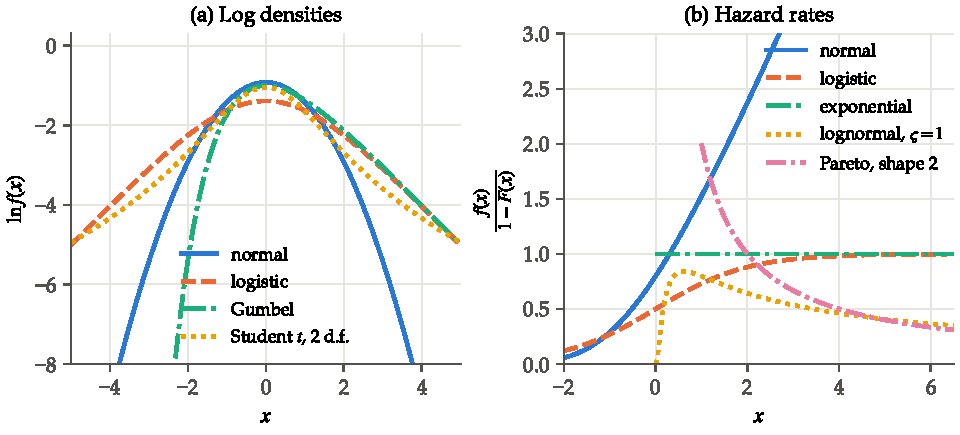
\includegraphics[width=\textwidth]{figures/appB/logconcave.pdf}
\caption{Log densities and hazard rates. Panel (a): $\ln f$ for the standard normal, standard logistic and
standard Gumbel densities, all concave, and for the Student $t$ density with two degrees of freedom, which is
convex in the tails. Panel (b): hazard rates $\frac{f(x)}{1 - F(x)}$. The normal and logistic hazards rise, the
unit exponential hazard is constant, the lognormal hazard with $\varsigma = 1$ peaks near $x = 0.62$ and then falls,
and the Pareto hazard $\frac{2}{x}$ falls.}
\label{fig:B-logconcave}
\end{figure}

\subsection{Pricing applications}\label{sec:B-lc-pricing}

\casehead{Monopoly}
Consider a single-product monopolist with constant marginal cost $c$ and differentiable demand $Q(p)$ that is
nonincreasing and positive on an interval $(c, \bar p)$, with $\bar p \leq \infty$ and $Q(p) = 0$ for $p \geq \bar p$.
Profit is $\pi(p) = (p - c)Q(p)$. Write $m(p) = -\frac{Q(p)}{Q'(p)}$ for the dollar markup that the first-order
condition supports at price $p$, the reciprocal of the semi-elasticity $-\frac{Q'}{Q}$ (\cref{ch:theory}).

\begin{proposition}[Log-concave demand and the monopoly problem]\label{prop:B-lc-monopoly}
Suppose $Q$ is log-concave on $(c, \bar p)$.
\begin{enumerate}[label=(\roman*)]
  \item Profit is log-concave on $(c, \bar p)$ and quasi-concave on $\R$, so the set of profit-maximizing prices
  is an interval.
  \item The first-order condition $p - c = m(p)$ has at most one solution in $(c, \bar p)$, and a solution is the
  global profit maximizer.
  \item Where $m$ is differentiable at the optimum, monopoly pass-through satisfies
  $\rho = \frac{1}{1 - m'(p)} \in (0, 1]$.
\end{enumerate}
If $Q$ is strictly log-concave, the maximizer is unique.
\end{proposition}

\begin{proof}
(i) On $(c, \bar p)$ profit is positive and $\ln\pi(p) = \ln(p - c) + \ln Q(p)$. Both terms are concave, so
$\ln\pi$ is concave. Outside $(c, \bar p)$ profit is nonpositive. Each upper contour set $\{p : \pi(p) \geq k\}$
with $k > 0$ is an upper contour set of the concave function $\ln\pi$, hence an interval. For $k \leq 0$ the set
contains all prices above $c$. It is an interval because profit is nondecreasing below $c$, where a higher price
shrinks both the loss per unit and the number of units sold.

(ii) Since $(\ln Q)' = \frac{Q'}{Q}$ is nonincreasing, the semi-elasticity $-\frac{Q'}{Q}$ is nondecreasing and
the markup $m(p)$ is nonincreasing where $Q' < 0$. The left side $p - c$ of the first-order condition is strictly
increasing. The two sides can cross at most once. A solution makes $(\ln\pi)'$ vanish, and a stationary point of a
concave function is a global maximizer on $(c, \bar p)$, where all positive profits are earned.

(iii) Differentiate the identity $p(c) - c = m(p(c))$ with respect to $c$:
\[
  \rho - 1 = m'(p)\rho.
\]
Solving gives $\rho = \frac{1}{1 - m'(p)}$, and $m' \leq 0$ gives $0 < \rho \leq 1$. Strict log-concavity makes $\ln\pi$
strictly concave, so the maximizer is unique.
\end{proof}

Part (iii) is the global counterpart of \cref{cor:B-passthrough-logconcave}. That corollary states that at the
monopoly price pass-through is below one if and only if $(\ln Q)'' < 0$ and above one if and only if $(\ln Q)'' > 0$. The
two statements agree because $m' = -1 + \frac{QQ''}{(Q')^2}$, so $\frac{1}{1 - m'} = \frac{1}{2 - \frac{QQ''}{(Q')^2}}$.

The proposition has a probabilistic reading. Suppose consumers have unit demand and their willingness to pay
$W$ has CDF $F_W$ and density $f_W$. Demand is $Q(p) = M[1 - F_W(p)]$ for market size $M$, and the markup is
$m(p) = \frac{1 - F_W(p)}{f_W(p)}$, the reciprocal of the hazard rate of $W$. Demand is log-concave exactly when
the survival function of $W$ is log-concave, that is, when $W$ has an increasing failure rate
(\cref{cor:B-hazard}). A log-concave density of willingness to pay suffices (\cref{prop:B-lc-cdf}). The same
object reappears as Myerson's virtual valuation in \cref{sec:B-lc-auctions}.

\casehead{Constant pass-through}
Pass-through usually varies with the level of cost. \citet{BulowPfleiderer1983} identify the demand curves for
which it does not. Let $P(q)$ be inverse demand with $P' < 0$ and curvature
$\chi(q) = -\frac{qP''(q)}{P'(q)}$, as in \eqref{eq:B-chi}. By \cref{prop:B-passthrough-monopoly}, monopoly
pass-through at output $q$ is $\rho = \frac{1}{2 - \chi(q)}$, and the second-order condition is $2 - \chi > 0$.

\begin{proposition}[Constant pass-through demands]\label{prop:B-constant-pt}
Let a monopolist with constant marginal cost face a twice continuously differentiable inverse demand with
$P' < 0$ and $2 - \chi > 0$ on an interval of outputs. Pass-through is the same at every cost in an interval of
costs if and only if inverse demand takes one of the two forms below on the corresponding interval of outputs.
\begin{enumerate}[label=(\alph*)]
  \item $P(q) = a - bq^\gamma$ with $b\gamma > 0$ and $\gamma > -1$, in which case $\rho = \frac{1}{1 + \gamma}$.
  \item $P(q) = a - b\ln q$ with $b > 0$, in which case $\rho = 1$.
\end{enumerate}
\end{proposition}

\Cref{prop:02-pt-constant} states the result in the same notation and leaves the converse as an exercise. The
proof below carries it out.

\begin{proof}
Monopoly output $q^*(c)$ is continuous and strictly decreasing, because the implicit function theorem gives
$\frac{\dd q^*}{\dd c} = \frac{1}{2P' + qP''} = \frac{1}{P'(2 - \chi)} < 0$. Hence $\rho = \frac{1}{2 - \chi(q^*(c))}$ is
constant on an interval of costs if and only if $\chi$ is constant on the image interval of outputs.

It remains to solve $qP''(q) = -\chi P'(q)$ for a constant $\chi$. Since $P' < 0$, write $-P'(q) = e^{\ell(q)}$. Then
$P'' = P'\ell'$, and the equation becomes $q\ell'(q) = -\chi$. Integrating $\ell'(q) = -\frac{\chi}{q}$ gives
$\ell(q) = -\chi\ln q + \ln K$ for a constant $K > 0$, so
\[
  P'(q) = -Kq^{-\chi}.
\]
If $\chi \neq 1$, integrate once more and set $\gamma = 1 - \chi$ and $b = \frac{K}{\gamma}$:
\[
  P(q) = a - \frac{K}{1 - \chi}q^{1 - \chi} = a - bq^\gamma,
\]
with $b\gamma = K > 0$. The second-order condition $2 - \chi > 0$ is $\gamma > -1$, and
$\rho = \frac{1}{2 - (1 - \gamma)} = \frac{1}{1 + \gamma}$. If $\chi = 1$, integrating $P' = -Kq^{-1}$ gives
$P(q) = a - K\ln q$, form (b) with $b = K$, and $\rho = \frac{1}{2 - 1} = 1$. Conversely, direct differentiation shows
that form (a) has $\chi = 1 - \gamma$ and form (b) has $\chi = 1$ at every output.
\end{proof}

The family contains the three textbook cases of \cref{ex:B-passthrough}. Linear demand is $\gamma = 1$ with
$\rho = \frac{1}{2}$. Constant-elasticity demand $P = q^{-\frac{1}{\varepsilon}}$ with $\varepsilon > 1$ is $a = 0$,
$b = -1$ and $\gamma = -\frac{1}{\varepsilon} \in (-1, 0)$, so $\rho = \frac{1}{1 - \frac{1}{\varepsilon}} = \frac{\varepsilon}{\varepsilon - 1} > 1$.
Exponential demand $Q = e^{\frac{a - p}{b}}$ is form (b) with $\rho = 1$. The family also sorts demand by
log-concavity. Since $\frac{QQ''}{(Q')^2} = \chi = 1 - \gamma$ (\cref{prop:B-passthrough-monopoly}), direct demand is strictly
log-concave when $\gamma > 0$, log-linear in form (b), and strictly log-convex when $-1 < \gamma < 0$. The ranking
of pass-through rates matches \cref{prop:B-lc-monopoly}.

\begin{example}[Power demand in prices]\label{ex:B-power-demand}
Let direct demand be $Q(p) = B(\bar p - p)^{g}$ for $p < \bar p$, with $B, g > 0$, as in \cref{tab:02-pt-examples}. Its
log is $\ln B + g\ln(\bar p - p)$, with second derivative $-\frac{g}{(\bar p - p)^2} < 0$, so demand is strictly
log-concave. Inverting $q = B(\bar p - p)^{g}$ gives
\[
  P(q) = \bar p - B^{-\frac{1}{g}}\,q^{\frac{1}{g}},
\]
which is form (a) with $a = \bar p$, $\gamma = \frac{1}{g}$ and $b = B^{-\frac{1}{g}}$. Directly, the first-order
condition $p - c = m(p)$ reads
\[
  p - c = \frac{\bar p - p}{g}.
\]
Solving gives $p = \frac{\bar p + gc}{1 + g}$, so $\rho = \frac{g}{1 + g} = \frac{1}{1 + \gamma}$, as
\cref{prop:B-constant-pt} predicts. Under a constant conduct parameter $\theta$ and flat marginal cost,
\cref{cor:B-passthrough-cases}(a) gives $\rho = \frac{1}{1 + \theta(1 - \chi)} = \frac{1}{1 + \theta\gamma} = \frac{1}{1 + \frac{\theta}{g}} = \frac{g}{g + \theta}$,
again independent of cost. This family appears in the sugar-refining application of \cref{ch:conduct}.
\end{example}

\begin{example}[Logit demand is log-concave]\label{ex:B-logit-lc}
Hold rivals' prices fixed and write single-product logit demand for product $j$ as
$s_j(p_j) = \frac{e^{\tilde\delta_j - \alpha p_j}}{\Lambda_{-j} + e^{\tilde\delta_j - \alpha p_j}}$, where $\tilde\delta_j$ is the
price-free part of mean utility and $\Lambda_{-j} = 1 + \sum_{l \neq j}e^{\delta_l}$ (\cref{sec:B-ev}).
Differentiating the log,
\[
  \frac{\dd\ln s_j}{\dd p_j} = -\alpha + \alpha s_j = -\alpha(1 - s_j),
\]
and differentiating again with $\frac{\dd s_j}{\dd p_j} = -\alpha s_j(1 - s_j)$,
\[
  \frac{\dd^2\ln s_j}{\dd p_j^2} = \alpha\frac{\dd s_j}{\dd p_j} = -\alpha^2s_j(1 - s_j) < 0.
\]
Residual demand is strictly log-concave. By \cref{prop:B-lc-monopoly}, each firm has a unique best response,
the solution of $p_j - mc_j = \frac{1}{\alpha(1 - s_j)}$ (\cref{prop:B-logit-br} gives it in closed form). Part
(iii) of the proposition puts own pass-through with rivals' prices fixed in $(0, 1]$, and
\cref{ex:B-passthrough}(iv) computes it exactly as $1 - s_j$.
\end{example}

\subsection{Aggregation and the existence of price equilibrium}\label{sec:B-caplin-nalebuff}

With several differentiated products, the existence of a pure-strategy Bertrand-Nash equilibrium requires each
firm's profit to be quasi-concave in its own price. Otherwise best responses can jump and Kakutani's theorem
fails. Demand is an aggregate over heterogeneous consumers, so the question is which primitives make aggregate
demand concave enough. \citet{CaplinNalebuff1991} answer it with \cref{thm:B-prekopa-borell}. \Cref{sec:04-cn}
proves their theorems and discusses their economic coverage. This subsection restates the argument as an
application of $\varrho$-concavity and refers to those proofs.

\casehead{Setting}
There are $J$ firms. Firm $j$ sells one product with fixed characteristics $x_j$ at constant marginal cost
$c_j$, and firms set prices simultaneously. Each consumer has income $y > 0$ and buys one unit of exactly one
product, consuming $z = y - p_j$ of a numeraire. Consumers differ by a type $\nu \in \R^L$ with density $f$ and
convex support $B$. The dimension $L$ of the type space is local to this subsection. \citet{CaplinNalebuff1991}
impose two assumptions.

\begin{assumption}[A1, preferences linear in the type]\label{ass:B-cn-a1}
Utility is $U(\nu, x, z) = \sum_{l=1}^L \nu_l t_l(x) + g(z)t_{L+1}(x) + t_{L+2}(x)$, where $t : X \to \R^{L+2}$ maps
characteristics into benefits, $g$ is strictly increasing and concave, and $t_{L+1}(x) > 0$.
\end{assumption}

\begin{assumption}[A2, concavity of the type density]\label{ass:B-cn-a2}
The density $f$ is $\varrho$-concave with $\varrho = -\frac{1}{L + 1}$, on a convex support with positive volume.
\end{assumption}

All consumers agree on the benefits $t_l(x)$ that a product delivers and differ in the weights $\nu_l$ they place on
them. By \cref{lem:B-rho-hierarchy}, every log-concave density satisfies A2. A2 also admits the multivariate
Cauchy, Pareto, F and Student $t$ distributions under restrictions on their parameters, for the Student $t$ at
least one degree of freedom \citep[Section 3, p.~6]{CaplinNalebuff1991}. A1 covers
characteristics models, quadratic transport costs, vertical differentiation, and logit, probit and random
coefficients models with a common price coefficient. It excludes Hotelling's linear transport costs, whose
demand is discontinuous.

\casehead{Demand as the probability of a set}
Fix rivals' prices $p_{-j}$. Let $\mathcal{A}_j(p_j)$ be the set of types that weakly prefer product $j$ at price
$p_j$ to every rival,
\[
  \mathcal{A}_j(p_j) = \bigl\{\nu : \Delta_k(\nu, p_j) \geq 0 \text{ for all } k \neq j\bigr\},
  \qquad \Delta_k(\nu, p_j) = U(\nu, x_j, y - p_j) - U(\nu, x_k, y - p_k)\text{.}
\]

Ties occur on hyperplanes of types when products are distinct, so they have probability zero. Demand is
\begin{equation}\label{eq:B-cn-demand}
  D_j(p_j) = \int_{\mathcal{A}_j(p_j)} f(\nu)\,\dd\nu,
\end{equation}
which is the demand function of \citet[Section 4]{CaplinNalebuff1991}, written with the set of buyers instead of
reservation prices. Given rivals' prices, firm $j$ is a monopolist facing a population of reservation prices.

\begin{lemma}[Buyer sets are Minkowski-concave]\label{lem:B-cn-minkowski}
Under A1, for any prices $p_0$, $p_1$ and $\lambda \in [0, 1]$, with $p_\lambda = \lambda p_0 + (1 - \lambda)p_1$,
\[
  \mathcal{A}_j(p_\lambda) \supseteq \lambda\mathcal{A}_j(p_0) + (1 - \lambda)\mathcal{A}_j(p_1).
\]
\end{lemma}

The proof of \cref{thm:04-cn-demand} establishes this inclusion. It averages the preference inequalities of
types $\nu_0$ and $\nu_1$, which A1 makes linear in the type, and uses concavity of $g$ for the price term.

\begin{theorem}[Aggregation, \citealp{CaplinNalebuff1991}, Section 4]\label{thm:B-cn-aggregation}
Assume A1, distinct products and a $\varrho$-concave type density with $\varrho \geq -\frac{1}{L}$. Then each firm's demand
$D_j(p_j)$ is $\varrho^*$-concave in its own price, with $\varrho^* = \frac{\varrho}{1 + L\varrho}$, on the interval of prices
where it is positive.
\end{theorem}

This is \cref{thm:04-cn-demand}. For prices $p_0$ and $p_1$ with positive demand, \cref{lem:B-cn-minkowski},
monotonicity of the integral and \cref{thm:B-prekopa-borell} give
\[
  D_j(p_\lambda) \geq \int_{\lambda\mathcal{A}_j(p_0) + (1 - \lambda)\mathcal{A}_j(p_1)} f(\nu)\,\dd\nu
  \geq \mathcal{M}_{\varrho^*}\bigl(D_j(p_0), D_j(p_1); \lambda\bigr).
\]
The bound is tight (\cref{ex:04-cn-simplex}). With types uniform on the unit simplex and reservation prices
$1 - \sum_l\nu_l$, demand is $D(p) = (1 - p)^L$, which is $\frac{1}{L}$-concave and no more.

\casehead{Quasi-concave profit}
The second step turns concavity of demand into quasi-concavity of profit.

\begin{proposition}[Convex reciprocal demand gives quasi-concave profit]\label{prop:B-cn-quasiconcave}
Let marginal cost $c$ be constant and let demand $D$ be nonincreasing, positive on an interval $(-\infty, \bar p)$
and zero above it. If $\frac{1}{D}$ is convex on $(-\infty, \bar p)$, then profit $\pi(p) = (p - c)D(p)$ is
quasi-concave.
\end{proposition}

\Cref{lem:04-recip} proves the result by contradiction, following \citet[p.~29]{CaplinNalebuff1991}. A direct
argument uses upper contour sets. For $k > 0$ and prices in $(c, \bar p)$, $\pi(p) \geq k$ holds if and only if
$p - c - \frac{k}{D(p)} \geq 0$. The left side is linear minus a convex function, hence concave, so its upper
contour set is an interval. For $k \leq 0$ the set contains every price above $c$, and profit is nondecreasing
below $c$.

For strictly decreasing, twice differentiable demand, $\frac{1}{D}$ is convex if and only if revenue $qP(q)$ is
concave in quantity (\cref{sec:04-existence-demand} gives the computation). \citet[Section 5]{CaplinNalebuff1991}
note that concave revenue is equivalent to quasi-concavity of profit for every convex cost function. The condition is therefore as weak as possible when costs are unrestricted. In the language of
\cref{def:B-rhoconcave}, $\frac{1}{D}$ convex means that $D$ is $(-1)$-concave. \Cref{thm:B-cn-aggregation}
delivers this when $\varrho^* \geq -1$. Solving $\frac{\varrho}{1 + L\varrho} = -1$ step by step,
\begin{align*}
  \varrho &= -(1 + L\varrho),\\
  \varrho(1 + L) &= -1,\\
  \varrho &= -\frac{1}{L + 1}.
\end{align*}
Because $\varrho^*$ is increasing in $\varrho$ and $-\frac{1}{L + 1} > -\frac{1}{L}$, every density that satisfies A2 yields
$\varrho^* \geq -1$, hence $(-1)$-concave demand by \cref{lem:B-rho-hierarchy}, hence quasi-concave profit. This
is why A2 has the exponent $-\frac{1}{L + 1}$. The same calculation shows why earlier work that assumed concave
demand was confined to special cases. Concave demand needs $\varrho^* = 1$, which requires $\varrho = \infty$ and
$L = 1$, a uniform distribution of types on a line \citep[Section 5]{CaplinNalebuff1991}.

\begin{theorem}[Existence, \citealp{CaplinNalebuff1991}, Section 5]\label{thm:B-cn-existence}
Under A1 and A2, for any number of firms and any products, a pure-strategy Bertrand-Nash equilibrium exists.
\end{theorem}

\Cref{thm:04-cn-existence} proves the theorem. With distinct products, it restricts each firm to prices in
$[c_j, y]$, where profits are continuous. Quasi-concavity in own price makes each best-response set an interval,
and Kakutani's theorem (\cref{thm:B-kakutani}) gives a fixed point. Equivalent products and costs above income
are handled separately.

\casehead{Uniqueness and log-supermodularity}
\citet[Section 6]{CaplinNalebuff1991} prove uniqueness under differentiability in three cases.
\begin{enumerate}[label=(\alph*)]
  \item Duopoly with a log-concave type density, in any dimension.
  \item Any number of firms in a one-dimensional market with a log-concave density, given the set of active firms.
  \item The logit model.
\end{enumerate}
The tool is the dominant-diagonal condition
$\bigl|\frac{\partial^2\pi_j}{\partial p_j^2}\bigr| > \sum_{k \neq j}\bigl|\frac{\partial^2\pi_j}{\partial p_j\,\partial p_k}\bigr|$, which
allows at most one equilibrium among a given set of active firms \citep{Friedman1977}
(\cref{prop:B-dd-uniqueness}). In all three cases the pricing game is also log-supermodular, a property
studied in \cref{sec:B-supermodular-games}.

The logit case was checked in \cref{sec:B-equilibrium}. There the log first-order conditions
$\frac{\partial\ln\pi_j}{\partial p_j} = \frac{1}{p_j - c_j} - \alpha(1 - s_j) = 0$ satisfy the dominant-diagonal condition on
the set of prices above cost. On the best response, the implicit function theorem turns the same derivatives into
the slopes $\frac{\partial BR_j}{\partial p_k} = \frac{s_js_k}{1 - s_j} > 0$, whose row sums are below one
(\cref{prop:B-logit-br-contraction}). Best responses slope up, so logit prices are strategic complements.

Log-supermodularity combined with uniqueness has strong consequences \citep{MilgromRoberts1990}. Caplin and
Nalebuff list four.
\begin{enumerate}[label=(\arabic*)]
  \item There are no other equilibria in mixed or correlated strategies.
  \item The equilibrium is globally stable under best-response dynamics, fictitious play and Bayesian learning.
  \item The game is dominance solvable.
  \item Any change that raises some firm's marginal return to price raises every firm's equilibrium price.
\end{enumerate}
A cost increase for one firm, for instance, raises all prices (\cref{ex:B-logit-cost}).

The theorem has limits. It assumes unit demand, single-product firms and fixed products. Multiproduct logit
pricing is unique by a different argument (\cref{sec:B-fixedpoint}). A random price coefficient fits A1 only
after utility is divided by it, and A2 must then hold for the distribution of the resulting ratios, which can fail
(\cref{sec:04-cn}).

Random price coefficients are often lognormal in random coefficients demand models, so the lognormal deserves a
check. \citet[Section 3, p.~6]{CaplinNalebuff1991} note that A2 survives the truncation of a density to a convex
support but not other transformations. They give the lognormal as a distribution that fails A2. The failure
depends on the dispersion. With $L = 1$, A2 requires $f^{-\frac{1}{2}}$ to be convex. Let $\ln\nu \sim N(m,
\varsigma^2)$ and write $t = \ln\nu$. Up to a positive constant, $f(\nu)^{-\frac{1}{2}} = e^{g(t)}$ with
\[
  g(t) = \frac{t}{2} + \frac{(t - m)^2}{4\varsigma^2}.
\]
Since $\frac{\dd}{\dd\nu} = \frac{1}{\nu}\frac{\dd}{\dd t}$, differentiating twice gives
\[
  \frac{\dd^2}{\dd\nu^2}e^{g(t)} = \frac{e^{g(t)}}{\nu^2}\bigl[g'(t)^2 - g'(t) + g''(t)\bigr]
  = \frac{e^{g(t)}}{\nu^2}\Bigl[\Bigl(g'(t) - \frac{1}{2}\Bigr)^2 - \frac{1}{4} + \frac{1}{2\varsigma^2}\Bigr].
\]
The derivative $g'(t) = \frac{1}{2} + \frac{t - m}{2\varsigma^2}$ takes every real value, so the bracket is nonnegative
everywhere exactly when $\frac{1}{2\varsigma^2} \geq \frac{1}{4}$, that is, when $\varsigma^2 \leq 2$. A
one-dimensional lognormal therefore satisfies A2 for moderate dispersion and fails it for large dispersion. Its
density is never log-concave (\cref{tab:B-logconcave}), so here A2 is a real gain over log-concavity.

\subsection{Auction applications}\label{sec:B-lc-auctions}

Hazard rates and reverse hazard rates are the natural objects in auction theory. The hazard rate governs the
seller's trade-off between price and probability of sale. The reverse hazard rate governs a bidder's trade-off
between the margin and the probability of winning. In this subsection a bidder's value has CDF $F$ with density
$f > 0$ on $[\underline v, \bar v]$, and the seller values the object at $v_0$.

\begin{proposition}[Myerson regularity]\label{prop:B-regular}
If the hazard rate $\frac{f}{1 - F}$ is nondecreasing, the virtual valuation
$\psi(v) = v - \frac{1 - F(v)}{f(v)}$ is strictly increasing, so $F$ is regular. A log-concave density suffices.
\end{proposition}

\begin{proof}
The term $\frac{1 - F}{f}$ is the reciprocal of a nondecreasing positive function, so it is nonincreasing. Then
$\psi$ is the sum of the strictly increasing function $v$ and the nondecreasing function $-\frac{1 - F}{f}$. A
log-concave density has a nondecreasing hazard rate by \cref{cor:B-hazard}.
\end{proof}

Regularity makes the optimal reserve price the unique solution of $r^* - \frac{1 - F(r^*)}{f(r^*)} = v_0$, because
the left side is strictly increasing \citep{Myerson1981}. For values uniform on $[0, 1]$,
$\psi(v) = v - (1 - v) = 2v - 1$ and $r^* = \frac{1 + v_0}{2}$. For exponential values with rate $\lambda$,
$\psi(v) = v - \frac{1}{\lambda}$ and $r^* = v_0 + \frac{1}{\lambda}$. The seller's problem with one bidder is the monopoly
problem of \cref{prop:B-lc-monopoly} with willingness to pay $V$ and cost $v_0$. \Cref{cor:14-optimal-reserve} in
\cref{ch:auction-theory} gives the general result.

Consider a symmetric first-price auction with independent private values and $N$ bidders. A bidder who bids $b$
must have value $\xi(b) = b + \frac{G(b)}{(N - 1)g(b)}$ \citep{GuerrePerrigneVuong2000}. Here $G$ and $g$ are the
distribution and density of equilibrium bids. \citet[Theorem 1]{GuerrePerrigneVuong2000} write $I$ for the number of
bidders. They show that an observed bid distribution is rationalized by some value distribution if and only if
bids are i.i.d.\ and $\xi$ is strictly increasing with a differentiable inverse. The second requirement is their
condition C2.

\begin{proposition}[Log-concave bids satisfy the monotonicity condition]\label{prop:B-gpv-monotone}
Let $G$ have a positive differentiable density $g$ on $[\underline b, \bar b]$. If $G$ is log-concave, then
$\xi(b) = b + \frac{G(b)}{(N - 1)g(b)}$ is strictly increasing. More generally, $\xi$ is strictly increasing if and
only if $\frac{g}{G^N}$ is strictly decreasing.
\end{proposition}

\begin{proof}
If $G$ is log-concave, the reverse hazard rate $\frac{g}{G}$ is nonincreasing (\cref{cor:B-hazard}), so
$\frac{G}{g}$ is nondecreasing. Then $\xi$ is the sum of the strictly increasing function $b$ and a nondecreasing
function. For the general statement, differentiate $\xi$ by the quotient rule:
\[
  \xi'(b) = 1 + \frac{g(b)^2 - G(b)g'(b)}{(N - 1)g(b)^2} = \frac{Ng(b)^2 - G(b)g'(b)}{(N - 1)g(b)^2}.
\]
Differentiating $\frac{g}{G^N}$ gives
\[
  \frac{\dd}{\dd b}\left(\frac{g}{G^N}\right) = \frac{g'G^N - NG^{N-1}g^2}{G^{2N}} = -\frac{Ng^2 - Gg'}{G^{N+1}}.
\]
The two derivatives have opposite signs. Hence $\xi' > 0$ exactly when $\frac{g}{G^N}$ is strictly decreasing
\citep[p.~530 and footnote 6]{GuerrePerrigneVuong2000}.
\end{proof}

Log-concavity is sufficient for condition C2 and far from necessary. A violation needs a bid density that
falls steeply relative to $G$. \citet[p.~530]{GuerrePerrigneVuong2000} give the example
$G(b) = \bigl(\frac{b}{5 - 4b}\bigr)^{\frac{1}{5}}$ on $[0, 1]$ with $N = 2$, whose density has a deep U shape. Here
$\frac{\dd\ln G}{\dd b} = \frac{1}{5}\bigl(\frac{1}{b} + \frac{4}{5 - 4b}\bigr) = \frac{1}{b(5 - 4b)}$, so
\[
  \xi(b) = b + b(5 - 4b) = 6b - 4b^2,
\]
which decreases for $b > \frac{3}{4}$. No independent private values model generates these bids. The
identification argument is developed in \cref{ch:auction-empirics}.

Reverse hazard rates also compare bidders. In an asymmetric auction, a strong bidder's value distribution $F_s$
and a weak bidder's $F_w$ are typically ranked by the reverse hazard rate. The ranking implies first-order
dominance.

\begin{proposition}[Reverse hazard rate dominance implies first-order dominance]\label{prop:B-rh-fosd}
Let $F_s$ and $F_w$ have positive densities $f_s$ and $f_w$ on a common support $[\underline v, \bar v]$. If
$\frac{f_s(v)}{F_s(v)} \geq \frac{f_w(v)}{F_w(v)}$ for all $v \in (\underline v, \bar v)$, then $F_s(v) \leq F_w(v)$ for all $v$.
\end{proposition}

\begin{proof}
Since $\frac{f}{F} = \frac{\dd}{\dd v}\ln F$, the hypothesis says
\[
  \frac{\dd}{\dd v}\ln\frac{F_s(v)}{F_w(v)} = \frac{f_s(v)}{F_s(v)} - \frac{f_w(v)}{F_w(v)} \geq 0,
\]
so the ratio $\frac{F_s}{F_w}$ is nondecreasing on $(\underline v, \bar v)$. Its limit at $\bar v$ is
$\frac{F_s(\bar v)}{F_w(\bar v)} = 1$. Hence $\frac{F_s(v)}{F_w(v)} \leq 1$, that is, $F_s(v) \leq F_w(v)$, for every
$v \in (\underline v, \bar v)$. At the endpoints both CDFs coincide.
\end{proof}

\Cref{sec:14-asym} extends the result to supports with different upper ends. The reverse hazard rate order is
the assumption under which \citet{MaskinRiley2000} sign equilibrium behavior in asymmetric first-price
auctions. The strong bidder shades its bid more, yet its bids are stochastically higher. The weak bidder sometimes
wins although its value is lower. \Cref{sec:B-stochastic-orders} places the order in the full chain of
stochastic orders.

\section{Supermodularity, monotone comparative statics and affiliation}\label{sec:B-supermod}

The implicit function theorem signs comparative statics through derivatives and second-order conditions
(\cref{prop:B-cs-optimum}). Many economic problems lack the smoothness or the concavity that this route needs.
Choices may be discrete, maximizers may jump, and profit functions may have several local peaks. Lattice
methods sign comparative statics from a single property, complementarity between the choice and the parameter,
and they extend to games and to probability. This section develops the order-theoretic tools and their uses in
oligopoly pricing, the vertical model and auctions. It ends with affiliation, the form of positive dependence that
auction theory uses.

\subsection{Lattices and supermodular functions}\label{sec:B-lattice}

We order $\R^k$ componentwise: $x \geq y$ means $x_l \geq y_l$ for every $l$. This is a \emph{partial order}, since two
vectors need not be comparable. The \emph{join} $x \vee y$ and the \emph{meet} $x \wedge y$ are the componentwise
maximum and minimum,
\[
  (x \vee y)_l = \max\{x_l, y_l\}, \qquad (x \wedge y)_l = \min\{x_l, y_l\}.
\]

\begin{definition}[Lattices]\label{def:B-lattice}
A set $X \subseteq \R^k$ is a \emph{lattice} (a sublattice of $\R^k$) if $x \vee y \in X$ and $x \wedge y \in X$ whenever
$x, y \in X$. A lattice is \emph{complete} if every nonempty subset has a supremum and an infimum in $X$.
\end{definition}

The whole space $\R^k$ and every product of intervals are lattices. A compact product of closed intervals is a
complete lattice. The set $\{x \in \R^2 : x_1 \leq x_2\}$ is a lattice, because the componentwise maximum and minimum
of two points with $x_1 \leq x_2$ inherit the inequality. The set $\{x \in \R^2 : x_1 + x_2 \leq 1\}$ is convex but not a
lattice: $(1, 0)$ and $(0, 1)$ belong to it, while their join $(1, 1)$ does not. Lattices are about order, convex
sets about averages, and the two notions are independent.

\begin{definition}[Supermodularity and increasing differences]\label{def:B-supermodular}
Let $X$ be a lattice and $A$ a partially ordered set of parameters.
\begin{enumerate}[label=(\roman*)]
  \item A function $g : X \to \R$ is \emph{supermodular} if $g(x \vee y) + g(x \wedge y) \geq g(x) + g(y)$ for all
  $x, y \in X$.
  \item A function $g : X \times A \to \R$ has \emph{increasing differences} in $(x, a)$ if, for all $x' \geq x$, the
  difference $g(x', a) - g(x, a)$ is nondecreasing in $a$. It has \emph{strictly increasing differences} if the
  difference is strictly increasing in $a$ whenever $x' > x$.
  \item A positive function $g$ is \emph{log-supermodular} if $\ln g$ is supermodular.
\end{enumerate}
\end{definition}

For two variables the two notions coincide. Take $x = (x_1', x_2)$ and $y = (x_1, x_2')$ with $x_1' \geq x_1$ and
$x_2' \geq x_2$. Then $x \vee y = (x_1', x_2')$ and $x \wedge y = (x_1, x_2)$, and supermodularity reads
\[
  g(x_1', x_2') - g(x_1, x_2') \geq g(x_1', x_2) - g(x_1, x_2),
\]
which says that the gain from raising the first variable is larger when the second is larger. Supermodularity is
the formal statement of complementarity. Ordered pairs impose nothing, because then $\{x \vee y, x \wedge y\} = \{x, y\}$.
For smooth functions on products of intervals there is a derivative test.

\begin{proposition}[Smooth test, \citealp{Topkis1978}]\label{prop:B-smooth-supermod}
Let $X = \prod_{l=1}^k I_l$ be a product of open intervals and let $g : X \to \R$ be twice continuously
differentiable. Then $g$ is supermodular if and only if $\frac{\partial^2g}{\partial x_l\,\partial x_m} \geq 0$ for all
$l \neq m$ at every point of $X$.
\end{proposition}

\begin{proof}
Suppose the cross partials are nonnegative and take $x, y \in X$. Let $z = x \wedge y$, $u = x - z \geq 0$ and
$w = y - z \geq 0$. A coordinate $l$ has $u_l > 0$ only if $x_l > y_l$, and $w_l > 0$ only if $y_l > x_l$, so $u$ and $w$
have disjoint supports. Moreover $x = z + u$, $y = z + w$ and $x \vee y = z + u + w$. We must show
\[
  g(z + u + w) - g(z + w) - g(z + u) + g(z) \geq 0\text{.}
\]
By the fundamental theorem of calculus along the segment from $z$ to $z + w$,
\[
  g(z + u + w) - g(z + w) - g(z + u) + g(z) = \int_0^1 \sum_m w_m\left[\frac{\partial g}{\partial x_m}(z + u + tw) - \frac{\partial g}{\partial x_m}(z + tw)\right]\dd t\text{.}
\]

Applying the theorem again along the segment from $z + tw$ to $z + u + tw$,
\[
  g(z + u + w) - g(z + w) - g(z + u) + g(z) = \int_0^1\!\!\int_0^1 \sum_m\sum_l w_mu_l\,\frac{\partial^2g}{\partial x_l\,\partial x_m}(z + su + tw)\,\dd s\,\dd t\text{.}
\]

Every term with $w_mu_l \neq 0$ has $l \neq m$ by disjointness, so it multiplies a nonnegative cross partial by a
nonnegative weight. The integral is nonnegative.

Conversely, suppose $g$ is supermodular and fix $l \neq m$, a point $x$, and small $\epsilon, \eta > 0$. Apply the
two-variable inequality above to coordinates $l$ and $m$ with the others held at $x$:
\[
  g(x + \epsilon e_l + \eta e_m) - g(x + \eta e_m) - g(x + \epsilon e_l) + g(x) \geq 0,
\]
where $e_l$ is the $l$-th unit vector. Divide by $\epsilon\eta$ and let $\epsilon, \eta \to 0$. By the double-integral
representation and continuity of the cross partial, the limit is $\frac{\partial^2g}{\partial x_l\,\partial x_m}(x) \geq 0$.
\end{proof}

The proposition applies to $\ln g$ as well. A positive $C^2$ function is log-supermodular if and only if
$\frac{\partial^2\ln g}{\partial x_l\,\partial x_m} \geq 0$ for $l \neq m$. Products of log-supermodular functions are
log-supermodular, because logs add. The same test applied to a function of $(x, a)$ with $x$ and $a$ scalars shows
that a $C^2$ function has increasing differences if and only if $\frac{\partial^2g}{\partial x\,\partial a} \geq 0$.

\subsection{Monotone comparative statics}\label{sec:B-topkis}

To compare sets of maximizers we need an order on sets.

\begin{definition}[Strong set order]\label{def:B-sso}
For subsets $S, S'$ of a lattice, $S'$ is higher than $S$ in the \emph{strong set order}, written $S' \geq_S S$, if
$x \vee x' \in S'$ and $x \wedge x' \in S$ for all $x \in S$ and $x' \in S'$.
\end{definition}

For compact intervals of $\R$, $S' \geq_S S$ means that $\max S' \geq \max S$ and $\min S' \geq \min S$. For general
compact subsets of $\R$ these inequalities are necessary but not sufficient. The sets $S = \{0, 2\}$ and $S' = \{1, 3\}$
satisfy both, yet $2 \vee 1 = 2 \notin S'$. For singletons it means $x' \geq x$.

\begin{theorem}[Topkis]\label{thm:B-topkis}
Let $X$ be a lattice, $A$ a partially ordered set, and $g : X \times A \to \R$ supermodular in $x$ for each $a$ and with
increasing differences in $(x, a)$. Let $M(a) = \argmax_{x \in X}g(x, a)$. If $a' \geq a$, then $M(a') \geq_S M(a)$. In
particular, the largest and smallest maximizers, when they exist, are nondecreasing in $a$ \citep{Topkis1978}.
\end{theorem}

\begin{proof}
Let $a' \geq a$, $x \in M(a)$ and $x' \in M(a')$. Both $x \vee x'$ and $x \wedge x'$ lie in $X$. Optimality of $x'$ at $a'$
and of $x$ at $a$ gives
\begin{align}
  g(x', a') &\geq g(x \vee x', a'), \label{eq:B-topkis-1}\\
  g(x, a) &\geq g(x \wedge x', a). \label{eq:B-topkis-2}
\end{align}
Supermodularity in $x$ at $a$, rearranged, and then \eqref{eq:B-topkis-2} give
\begin{equation}\label{eq:B-topkis-3}
  g(x \vee x', a) - g(x', a) \geq g(x, a) - g(x \wedge x', a) \geq 0.
\end{equation}
Since $x \vee x' \geq x'$ and $a' \geq a$, increasing differences give
\begin{equation}\label{eq:B-topkis-4}
  g(x \vee x', a') - g(x', a') \geq g(x \vee x', a) - g(x', a).
\end{equation}
Chaining \eqref{eq:B-topkis-4} and \eqref{eq:B-topkis-3}, $g(x \vee x', a') \geq g(x', a')$. With
\eqref{eq:B-topkis-1} this holds with equality, so $x \vee x' \in M(a')$. The left side of \eqref{eq:B-topkis-4} is
then zero, so every term in the chain is zero. In particular $g(x, a) = g(x \wedge x', a)$, and $x \wedge x' \in M(a)$.
\end{proof}

With strictly increasing differences and a scalar choice, every selection from the argmax is nondecreasing. To
see this, suppose $a' > a$, $x \in M(a)$, $x' \in M(a')$ and $x > x'$. Strictly increasing differences and optimality of $x$
at $a$ give $g(x, a') - g(x', a') > g(x, a) - g(x', a) \geq 0$, which contradicts optimality of $x'$ at $a'$.

Compare the theorem with \cref{prop:B-cs-optimum}. The implicit function theorem gives
$\frac{\dd x^*}{\dd a} = -\frac{g_{xa}}{g_{xx}}$, whose sign is that of $g_{xa}$ under a strict second-order condition.
Topkis's theorem reaches the qualitative conclusion from $g_{xa} \geq 0$ alone. It needs no concavity, no
differentiability in $x$, no interior solution and no uniqueness, and the choice set may be discrete. It is silent
on magnitudes, which still require derivatives.

The conditions of \cref{thm:B-topkis} are cardinal: a monotone transformation of $g$ can destroy increasing
differences without changing any argmax. \citet{MilgromShannon1994} found the ordinal conditions. A function
$g : X \to \R$ is \emph{quasi-supermodular} if $g(x) \geq g(x \wedge y)$ implies $g(x \vee y) \geq g(y)$, and the same holds
with strict inequalities. A function $g(x, a)$ satisfies the \emph{single crossing property} in $(x, a)$ if, for
$x' > x$ and $a' > a$, $g(x', a) \geq g(x, a)$ implies $g(x', a') \geq g(x, a')$, and $g(x', a) > g(x, a)$ implies
$g(x', a') > g(x, a')$. A gain from a higher choice at a low parameter persists at a higher parameter.

\begin{theorem}[\citealp{MilgromShannon1994}]\label{thm:B-milgrom-shannon}
Let $X$ be a lattice and $g : X \times A \to \R$. The following statements are equivalent.
\begin{enumerate}[label=(\alph*)]
  \item The set $\argmax_{x \in S}g(x, a)$ is nondecreasing in $(a, S)$ in the strong set order, over all sublattices
  $S \subseteq X$.
  \item The function $g$ is quasi-supermodular in $x$ and satisfies the single crossing property in $(x, a)$.
\end{enumerate}
\end{theorem}

Both conditions are preserved by strictly increasing transformations of $g$. A positive log-supermodular
function satisfies them. Indeed, if $\ln g$ has increasing differences, the ratio $\frac{g(x', a)}{g(x, a)}$ is
nondecreasing in $a$ for $x' \geq x$. If it is at least one at $a$, it is at least one at $a' > a$, which is single
crossing. This is why log-supermodularity, a cardinal condition on $\ln g$, has ordinal consequences for $g$.

\begin{example}[Monopoly price rises with cost for any demand]\label{ex:B-topkis-monopoly}
Let demand $Q(p)$ be any nonincreasing function on a price set $X = [0, \bar p]$, and let profit be
$\pi(p, c) = (p - c)Q(p)$. For $p' > p$,
\[
  \pi(p', c) - \pi(p, c) = p'Q(p') - pQ(p) - c\bigl[Q(p') - Q(p)\bigr].
\]
The bracket is nonpositive, so the difference is nondecreasing in $c$. Profit has increasing differences in
$(p, c)$, and by \cref{thm:B-topkis} the largest and smallest optimal prices are nondecreasing in marginal cost.
If $Q$ is strictly decreasing the differences are strictly increasing, and every selection of optimal prices is
nondecreasing. No curvature, concavity, continuity or differentiability of demand is used. On prices above cost,
the same conclusion follows from log-supermodularity, since
$\frac{\partial^2}{\partial p\,\partial c}\ln[(p - c)Q(p)] = \frac{\partial^2}{\partial p\,\partial c}\ln(p - c) = \frac{1}{(p - c)^2} > 0$.
The direction of pass-through is thus a free result, while its size, $\rho = \frac{1}{2 - \chi}$, depends on demand
curvature (\cref{sec:B-passthrough}).
\end{example}

\begin{example}[Sorting in the vertical model]\label{ex:B-vertical-sorting}
In the vertical model consumer $i$ obtains $u_{ij} = \delta_j - \nu_ip_j$ from product $j$, with $\nu_i > 0$ the price
sensitivity and the outside good at $\delta_0 = p_0 = 0$ (\cref{sec:06-vertical}). Index the products with positive
sales by price, $0 = p_0 < p_1 < \dots < p_J$, so that qualities rise in the same order. For $k > j$,
\[
  u_{ij} - u_{ik} = (\delta_j - \delta_k) + \nu_i(p_k - p_j),
\]
which is strictly increasing in $\nu_i$. This is the \emph{single crossing property} of the vertical model. As
functions of $\nu$, the utility lines of two products cross at most once, and the cheaper product wins for the
more price-sensitive consumers. In lattice terms, $u(j, \nu) = \delta_j - \nu p_j$ has strictly decreasing differences
in $(j, \nu)$, so by \cref{thm:B-topkis} applied with $-\nu$ as the parameter, the chosen product is nonincreasing in $\nu$.

Single crossing also explains why a consumer need compare product $j$ only with its two neighbors. Let
$\bar\nu_j = \frac{\delta_j - \delta_{j-1}}{p_j - p_{j-1}}$ be the type indifferent between $j - 1$ and $j$, and suppose the cutoffs
are strictly decreasing, $\bar\nu_1 > \bar\nu_2 > \dots > \bar\nu_J > 0$, as they are when every product sells. A
consumer prefers $j$ to $j + 1$ if and only if $\nu_i > \bar\nu_{j+1}$, and $j$ to $j - 1$ if and only if
$\nu_i < \bar\nu_j$. Suppose both hold. Then $\nu_i > \bar\nu_{j+1} > \bar\nu_{j+2}$, so she also prefers $j + 1$ to $j + 2$.
Transitivity gives $j \succ j + 2$, and induction on $k$ gives $j \succ k$ for all $k > j$. Symmetrically,
$\nu_i < \bar\nu_j < \bar\nu_{j-1}$ gives $j - 1 \succ j - 2$, hence $j \succ j - 2$ and, by induction, $j \succ k$ for all $k < j$.
With the conventions $\bar\nu_0 = \infty$ and $\bar\nu_{J+1} = 0$, the consumer chooses $j$ exactly when
$\bar\nu_{j+1} < \nu_i < \bar\nu_j$.
\end{example}

\begin{example}[Cournot best responses without concavity]\label{ex:B-cournot-topkis}
In a homogeneous-good Cournot market, firm $i$'s profit is $\pi_i(q_i, Q_{-i}) = q_iP(q_i + Q_{-i}) - C_i(q_i)$, where
$Q_{-i}$ is rivals' total output. \Cref{ex:B-cournot-br} computed the slope of the best response by the implicit
function theorem, under a strict second-order condition. The lattice argument needs only the cross partial,
\[
  \frac{\partial^2\pi_i}{\partial q_i\,\partial Q_{-i}} = P'(Q) + q_iP''(Q).
\]
If $P' + q_iP'' \leq 0$ on the relevant domain, profit has decreasing differences in $(q_i, Q_{-i})$, which are
increasing differences in $(q_i, -Q_{-i})$. By \cref{thm:B-topkis}, the extremal best responses are nonincreasing in
rivals' output. Neither concavity of profit in $q_i$ nor convexity of cost is needed, and the best response may be a
correspondence. \Cref{sec:B-strategic} shows that the sign of $P' + q_iP''$ can reverse.
\end{example}

\subsection{Strategic substitutes and complements}\label{sec:B-strategic}

\citet{BulowGeanakoplosKlemperer1985} sort competition by the sign of a single cross partial. Orient each
firm's strategic variable so that a higher value is more aggressive: quantities, advertising, or the negative of
a price.

\begin{definition}[Strategic substitutes and complements]\label{def:B-strategic}
Firm $B$ regards the products as \emph{strategic substitutes} if a more aggressive action by firm $A$ lowers $B$'s
marginal profit, that is, $\frac{\partial^2\pi_B}{\partial S_B\,\partial S_A} < 0$. It regards them as \emph{strategic
complements} if the cross partial is positive \citep[p.~494]{BulowGeanakoplosKlemperer1985}.
\end{definition}

The definition concerns marginal profit. Ordinary substitutes and complements concern the level of profit, the
sign of $\frac{\partial\pi_B}{\partial S_A}$. Under strict concavity in own action, the implicit function theorem gives
the slope of $B$'s best response (reaction function) $BR_B$,
\[
  \frac{\dd BR_B}{\dd S_A} = -\left(\frac{\partial^2\pi_B}{\partial S_B^2}\right)^{-1}\frac{\partial^2\pi_B}{\partial S_B\,\partial S_A}\text{.}
\]
Reaction curves therefore slope down under strategic substitutes and up under strategic complements. When prices are
the strategic variables, $S = -p$ and $\frac{\partial^2\pi_B}{\partial(-p_B)\,\partial(-p_A)} = \frac{\partial^2\pi_B}{\partial p_B\,\partial p_A}$, so
prices are strategic complements when $\frac{\partial^2\pi_B}{\partial p_B\,\partial p_A} > 0$.

\begin{example}[Multimarket contact and the sign of the strategic effect]\label{ex:B-bgk}
\citet[pp.~492--495]{BulowGeanakoplosKlemperer1985} study a firm $A$ that is a monopolist in market 1 and a duopolist
with firm $B$ in market 2. The strategic variables are $S_1^A$, $S_2^A$ and $S_2^B$. A shock $Z$ raises $A$'s marginal
profit in market 1, so $\pi^A = R_1^A(S_1^A) + R_2^A(S_2^A, S_2^B) - C^A(S_1^A, S_2^A) + ZS_1^A$ and
$\pi^B = R_2^B(S_2^A, S_2^B) - C^B(S_2^B)$, where $R_i^F$ is firm $F$'s revenue in market $i$ and $C^F$ its cost.
Shared costs make the markets interdependent. There are \emph{joint
economies} if $\frac{\partial^2\pi^A}{\partial S_1^A\,\partial S_2^A} > 0$ and joint diseconomies if it is negative. Write
$a_{11}$, $a_{12}$, $a_{22}$ and $a_{23}$ for the second partials of $\pi^A$ with respect to $(S_1^A, S_1^A)$,
$(S_1^A, S_2^A)$, $(S_2^A, S_2^A)$ and $(S_2^A, S_2^B)$. Write $b_{32}$ and $b_{33}$ for the second partials of $\pi^B$
with respect to $(S_2^B, S_2^A)$ and $(S_2^B, S_2^B)$. Totally differentiating the three first-order conditions gives their system
(7),
\[
  \begin{pmatrix} a_{11} & a_{12} & 0\\ a_{12} & a_{22} & a_{23}\\ 0 & b_{32} & b_{33}\end{pmatrix}
  \begin{pmatrix} \dd S_1^A\\ \dd S_2^A\\ \dd S_2^B\end{pmatrix}
  = \begin{pmatrix} -\dd Z\\ 0\\ 0\end{pmatrix}.
\]
The zero in the first row holds because $S_2^B$ affects $\pi^A$ only through market 2. Stability requires
$b_{33} < 0$, $a_{22}b_{33} > a_{23}b_{32}$ (market 2 is stable on its own) and a negative determinant. We solve from the
bottom. The third row gives $\dd S_2^B = -\frac{b_{32}}{b_{33}}\dd S_2^A$. Substituting into the second row,
\[
  a_{12}\,\dd S_1^A + k\,\dd S_2^A = 0, \qquad k \equiv a_{22} - \frac{a_{23}b_{32}}{b_{33}} = \frac{a_{22}b_{33} - a_{23}b_{32}}{b_{33}} < 0.
\]
Substituting $\dd S_2^A = -\frac{a_{12}}{k}\dd S_1^A$ into the first row gives
$\bigl(a_{11} - \frac{a_{12}^2}{k}\bigr)\dd S_1^A = -\dd Z$. The determinant equals $b_{33}(a_{11}k - a_{12}^2)$, which is
negative, so $a_{11}k - a_{12}^2 > 0$ and $a_{11} - \frac{a_{12}^2}{k} < 0$. Three results follow.
\begin{enumerate}[label=(\arabic*)]
  \item $\frac{\dd S_1^A}{\dd Z} > 0$: $A$ is more aggressive in the market whose profitability rose.
  \item $\operatorname{sign}\frac{\dd S_2^A}{\dd Z} = \operatorname{sign}(a_{12})$: with joint economies $A$ also becomes more
  aggressive in market 2.
  \item $\operatorname{sign}\frac{\dd S_2^B}{\dd Z} = \operatorname{sign}(a_{12})\cdot\operatorname{sign}(b_{32})$: $B$'s response depends on the
  joint economies and on whether $B$ regards the products as strategic substitutes or complements.
\end{enumerate}
By the envelope theorem (\cref{thm:B-envelope}), $\frac{\dd\pi^A}{\dd Z} = S_1^A + \frac{\partial\pi^A}{\partial S_2^B}\frac{\dd S_2^B}{\dd Z}$.
The second term is the \emph{strategic effect}. With ordinary substitutes, $\frac{\partial\pi^A}{\partial S_2^B} < 0$, its sign is
$-\operatorname{sign}(a_{12})\operatorname{sign}(b_{32})$. It is positive under joint economies with strategic substitutes or joint
diseconomies with strategic complements, and negative in the other two cases, as in their table on p.~495.
The same favorable shock can hurt a firm through its rival's response.
\end{example}

\begin{example}[Three oligopoly games]\label{ex:B-strategic-examples}
\leavevmode
\begin{enumerate}[label=(\alph*)]
  \item \emph{Cournot with linear demand.} With $P(Q) = a_0 - Q$, $P' + q_iP'' = -1 < 0$, so quantities are strategic
  substitutes everywhere.
  \item \emph{Cournot with constant-elasticity demand.} Let $P(Q) = Q^{-\frac{1}{\varepsilon}}$ with $\varepsilon > 0$. Then
  $P'(Q) = -\frac{1}{\varepsilon}Q^{-\frac{1}{\varepsilon} - 1}$ and $\frac{P''(Q)}{P'(Q)} = -\frac{1 + \frac{1}{\varepsilon}}{Q} = -\frac{1 + \varepsilon}{\varepsilon Q}$.
  With the share $s_i = \frac{q_i}{Q}$,
  \[
    P' + q_iP'' = P'\left[1 + q_i\frac{P''}{P'}\right] = P'\left[1 - \frac{1 + \varepsilon}{\varepsilon}s_i\right].
  \]
  Since $P' < 0$, the cross partial is positive, and firm $i$ treats quantities as strategic complements, exactly
  when $s_i > \frac{\varepsilon}{1 + \varepsilon}$. A firm with a small share regards rival output as a strategic
  substitute, while a firm with a large share regards it as a complement, as
  \citet[p.~494]{BulowGeanakoplosKlemperer1985} note.
  \item \emph{Logit Bertrand.} With single-product logit demand, $\ln\pi_j = \ln(p_j - mc_j) + \ln s_j(p)$ and
  \[
    \frac{\partial\ln\pi_j}{\partial p_j} = \frac{1}{p_j - mc_j} - \alpha(1 - s_j),
    \qquad
    \frac{\partial^2\ln\pi_j}{\partial p_j\,\partial p_k} = \alpha\frac{\partial s_j}{\partial p_k} = \alpha^2s_js_k > 0.
  \]
  Log profit has increasing differences in every pair of prices, so the logit pricing game is log-supermodular
  everywhere, and prices are strategic complements.
\end{enumerate}
Strategic complementarity among the prices of close substitutes is one reason a merger can raise the prices of
non-merging rivals. The MillerCoors joint venture of June 2008 tests how far this reason goes. Soon after it was
cleared, the prices of Miller Lite, Coors Light and Bud Light rose by about 8 percent. The prices of Corona Extra
and Heineken showed little persistent change \citep[pp.~241--242]{AskerNocke2021}. Unilateral effects could
produce this pattern only with extreme strategic complementarity between Bud Light and the MillerCoors brands,
together with weak substitution toward imports. \citet[p.~242]{AskerNocke2021} judge that combination unlikely.
\citet{MillerWeinberg2017} estimate a random coefficients nested logit demand and add a coordination parameter to
the ownership matrix of the pricing first-order conditions. Its estimate rejects unilateral Bertrand pricing, and
the coordinated-effects model fits the observed price paths \citep[p.~242 and fn.~164]{AskerNocke2021}. The
chapter on mergers develops the case (\cref{ch:mergers}).
\end{example}

\Cref{fig:B-reaction} contrasts the two cases. In the Cournot game, a cost reduction for firm 1 shifts its
reaction curve out, and the rival responds by producing less. In the Bertrand game with differentiated products,
a cost increase for firm 1 shifts its reaction curve out, and the rival responds by raising its price too.

Panel (b) uses the linear demand example of \citet[Section~11.2]{Tirole1988}. Firm $i$ sells
$q_i = 1 - bp_i + dp_j$ with $0 < d < b$, at constant unit cost $c$. Its profit $(p_i - c)(1 - bp_i + dp_j)$ is
concave in $p_i$, and the first-order condition is
\[
  1 + dp_j + bc - 2bp_i = 0, \qquad\text{so}\qquad BR_i(p_j) = \frac{1 + bc + dp_j}{2b}.
\]
The slope $\frac{d}{2b}$ is positive, so prices are strategic complements. It is below one half, so the
reaction curves cross once. Setting $p_i = p_j = p$ gives $2bp = 1 + bc + dp$, and the unique equilibrium is
symmetric,
\[
  p = \frac{1 + bc}{2b - d}.
\]
With $b = 1$, $d = \frac{1}{2}$ and $c = 0$, the best response is $\frac{1}{2} + \frac{1}{4}p_j$ and the equilibrium
price is $\frac{1}{2 - \frac{1}{2}} = \frac{2}{3}$, the point $N$ in the figure.

\begin{figure}[htbp]
\centering
\begin{subfigure}[t]{0.48\textwidth}
\centering
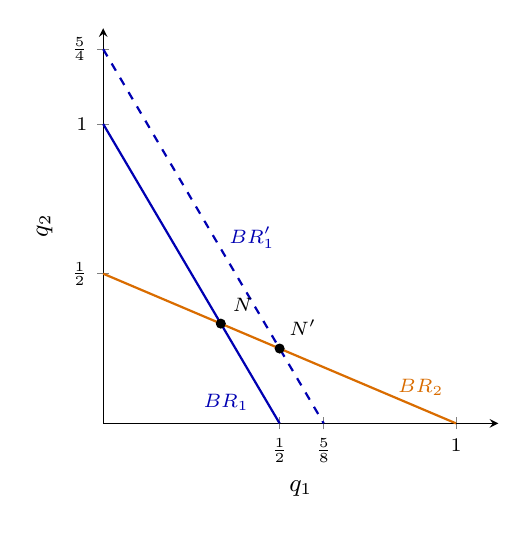
\begin{tikzpicture}
\begin{axis}[
  width=6.6cm, height=6.6cm,
  xmin=0, xmax=1.12, ymin=0, ymax=1.32,
  axis lines=left,
  xlabel={$q_1$}, ylabel={$q_2$},
  xtick={0.5,0.625,1}, xticklabels={$\frac{1}{2}$,$\frac{5}{8}$,$1$},
  ytick={0.5,1,1.25}, yticklabels={$\frac{1}{2}$,$1$,$\frac{5}{4}$},
  tick label style={font=\scriptsize}, label style={font=\small},
  clip=false]
  \addplot[blue!70!black, thick, domain=0:0.5, samples=2] {1-2*x};
  \addplot[blue!70!black, thick, dashed, domain=0:0.625, samples=2] {1.25-2*x};
  \addplot[orange!85!black, thick, domain=0:1, samples=2] {(1-x)/2};
  \addplot[only marks, mark=*, mark size=1.6pt] coordinates {(0.3333,0.3333) (0.5,0.25)};
  \node[font=\scriptsize, anchor=south west] at (axis cs:0.34,0.34) {$N$};
  \node[font=\scriptsize, anchor=south west] at (axis cs:0.5,0.26) {$N'$};
  \node[font=\scriptsize, anchor=east, blue!70!black] at (axis cs:0.44,0.07) {$BR_1$};
  \node[font=\scriptsize, anchor=west, blue!70!black] at (axis cs:0.33,0.62) {$BR_1'$};
  \node[font=\scriptsize, anchor=south, orange!85!black] at (axis cs:0.9,0.06) {$BR_2$};
\end{axis}
\end{tikzpicture}
\caption{Cournot: strategic substitutes}
\end{subfigure}\hfill
\begin{subfigure}[t]{0.48\textwidth}
\centering
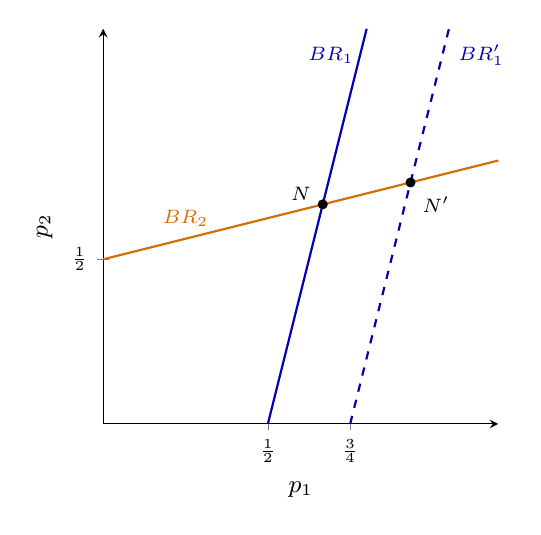
\begin{tikzpicture}
\begin{axis}[
  width=6.6cm, height=6.6cm,
  xmin=0, xmax=1.2, ymin=0, ymax=1.2,
  axis lines=left,
  xlabel={$p_1$}, ylabel={$p_2$},
  xtick={0.5,0.75}, xticklabels={$\frac{1}{2}$,$\frac{3}{4}$},
  ytick={0.5}, yticklabels={$\frac{1}{2}$},
  tick label style={font=\scriptsize}, label style={font=\small},
  clip=false]
  \addplot[blue!70!black, thick, domain=0.5:0.8, samples=2] {4*(x-0.5)};
  \addplot[blue!70!black, thick, dashed, domain=0.75:1.05, samples=2] {4*(x-0.75)};
  \addplot[orange!85!black, thick, domain=0:1.2, samples=2] {0.5+x/4};
  \addplot[only marks, mark=*, mark size=1.6pt] coordinates {(0.6667,0.6667) (0.9333,0.7333)};
  \node[font=\scriptsize, anchor=east] at (axis cs:0.66,0.70) {$N$};
  \node[font=\scriptsize, anchor=north west] at (axis cs:0.94,0.72) {$N'$};
  \node[font=\scriptsize, anchor=east, blue!70!black] at (axis cs:0.79,1.12) {$BR_1$};
  \node[font=\scriptsize, anchor=west, blue!70!black] at (axis cs:1.05,1.12) {$BR_1'$};
  \node[font=\scriptsize, anchor=south, orange!85!black] at (axis cs:0.25,0.57) {$BR_2$};
\end{axis}
\end{tikzpicture}
\caption{Differentiated Bertrand: strategic complements}
\end{subfigure}
\caption{Reaction curves under strategic substitutes and complements. Panel (a): Cournot duopoly with inverse
demand $P = a_0 - Q$ and $a_0 - c = 1$, so $BR_i(q_j) = \frac{1 - q_j}{2}$ and the equilibrium is
$N = (\frac{1}{3}, \frac{1}{3})$. A cost reduction of $\frac{1}{4}$ for firm 1 shifts its curve to
$BR_1'(q_2) = \frac{5}{8} - \frac{q_2}{2}$, and the new equilibrium is $N' = (\frac{1}{2}, \frac{1}{4})$: firm 2
contracts. Panel (b): the demand of \citet[Section~11.2]{Tirole1988} with $b = 1$ and $d = \frac{1}{2}$,
$q_i = 1 - p_i + \frac{1}{2}p_j$, with zero cost, so
$BR_i(p_j) = \frac{1}{2} + \frac{1}{4}p_j$ and $N = (\frac{2}{3}, \frac{2}{3})$. Raising firm 1's cost to $\frac{1}{2}$ shifts
its curve to $BR_1'(p_2) = \frac{3}{4} + \frac{1}{4}p_2$, and the new equilibrium is
$N' = (\frac{14}{15}, \frac{11}{15})$: both prices rise.}
\label{fig:B-reaction}
\end{figure}

\subsection{Supermodular games}\label{sec:B-supermodular-games}

Games with strategic complements have a lattice structure that delivers existence, computation and comparative
statics with no concavity and no differentiability. The fixed-point theorem behind them is due to Tarski.

\begin{theorem}[Tarski]\label{thm:B-tarski}
Let $\mathcal{X}$ be a complete lattice and $T : \mathcal{X} \to \mathcal{X}$ a nondecreasing map, that is, $x \leq x'$ implies
$T(x) \leq T(x')$. Then $T$ has a fixed point. Its largest fixed point is $\sup\{x \in \mathcal{X} : x \leq T(x)\}$, and the set
of fixed points is itself a complete lattice \citep{Tarski1955}.
\end{theorem}

\begin{proof}[Proof of existence]
Let $\mathcal{S} = \{x \in \mathcal{X} : x \leq T(x)\}$. It is nonempty because it contains $\inf\mathcal{X}$. Let
$\bar x = \sup\mathcal{S}$. For any $x \in \mathcal{S}$, $x \leq \bar x$, so $x \leq T(x) \leq T(\bar x)$. Thus $T(\bar x)$ is an
upper bound of $\mathcal{S}$, and $\bar x \leq T(\bar x)$. Applying $T$ gives $T(\bar x) \leq T(T(\bar x))$, so
$T(\bar x) \in \mathcal{S}$ and $T(\bar x) \leq \bar x$. Hence $T(\bar x) = \bar x$. Every fixed point lies in $\mathcal{S}$,
so $\bar x$ is the largest.
\end{proof}

Unlike Brouwer's and Kakutani's theorems, Tarski's theorem needs no continuity and no convexity. Monotonicity
does all the work.

\begin{definition}[Supermodular game]\label{def:B-smgame}
A game with players $i = 1, \dots, N$, strategy sets $X_i$ and payoffs $u_i(x_i, x_{-i})$ is \emph{supermodular} if
three conditions hold. Each $X_i$ is a compact product of intervals in some $\R^{k_i}$. Each $u_i$ is upper
semicontinuous in $x_i$ and continuous in $x_{-i}$. Each $u_i$ is supermodular in $x_i$ and has increasing differences
in $(x_i, x_{-i})$.
\end{definition}

Supermodularity in own strategy is automatic when each $x_i$ is a scalar. Increasing differences in
$(x_i, x_{-i})$ is strategic complementarity.

\begin{theorem}[Supermodular games]\label{thm:B-smgames}
In a supermodular game the following hold.
\begin{enumerate}[label=(\roman*)]
  \item The set of pure-strategy Nash equilibria is nonempty. It has a largest element $\bar x$ and a smallest
  element $\underline x$.
  \item Best-response iteration from the largest strategy profile, choosing the largest best response at each
  step, decreases monotonically to $\bar x$. Iteration from the smallest profile increases to $\underline x$.
  \item Suppose each $u_i(x_i, x_{-i}; a)$ has increasing differences in $(x_i, a)$ for a parameter $a$. Then $\bar x(a)$
  and $\underline x(a)$ are nondecreasing in $a$.
  \item Every strategy that survives iterated elimination of strictly dominated strategies lies between
  $\underline x$ and $\bar x$. A game with a unique equilibrium is therefore dominance solvable, and adaptive dynamics
  converge to it.
\end{enumerate}
\end{theorem}

\begin{proof}[Proof sketch]
(i) By \cref{thm:B-topkis}, applied with $x_{-i}$ as the parameter, player $i$'s set of best responses has a largest
element $\bar b_i(x_{-i})$, nondecreasing in $x_{-i}$. Upper semicontinuity and compactness ensure the set is
nonempty and has a largest element. The map $\bar b = (\bar b_1, \dots, \bar b_N)$ is a nondecreasing self-map of the
complete lattice $\prod_iX_i$. By \cref{thm:B-tarski} it has a largest fixed point $\bar x$, which is an equilibrium. If
$x^*$ is any equilibrium, then $x_i^* \leq \bar b_i(x_{-i}^*)$ for every $i$, so $x^* \leq \bar b(x^*)$ and $x^* \leq \bar x$ by the
characterization in \cref{thm:B-tarski}. The smallest equilibrium is symmetric.

(ii) Let $x^{(0)} = \sup\prod_iX_i$ and $x^{(h+1)} = \bar b(x^{(h)})$. Trivially $x^{(1)} \leq x^{(0)}$, and monotonicity of
$\bar b$ gives $x^{(h+1)} \leq x^{(h)}$ by induction. Similarly $\bar x \leq x^{(0)}$ implies $\bar x = \bar b(\bar x) \leq x^{(h)}$
for all $h$. The decreasing sequence converges, and continuity of payoffs makes its limit an equilibrium. The
limit is at least $\bar x$, so it equals $\bar x$.

(iii) If $a' \geq a$, then $\bar b(x; a') \geq \bar b(x; a)$ for every $x$ by \cref{thm:B-topkis}. Any $x$ with $x \leq \bar b(x; a)$
then satisfies $x \leq \bar b(x; a')$. The set whose supremum defines the largest fixed point grows with $a$, so its
supremum rises. Part (iv) is due to \citet{MilgromRoberts1990}.
\end{proof}

The results are due to \citet{Topkis1979}, \citet{Vives1990} and \citet{MilgromRoberts1990}, and \citet{Vives1999}
develops the oligopoly applications. When payoffs are positive, the theorem applies to a game with
log-supermodular payoffs after replacing $u_i$ by $\ln u_i$, because the transformation leaves best responses unchanged.

\begin{example}[A cost increase raises all logit prices]\label{ex:B-logit-cost}
Consider the single-product logit pricing game, and fix an interval of firm 1's costs
$[\underline{mc}_1, \overline{mc}_1]$ of length below $\frac{1}{\alpha}$. Every best response carries a markup
$\frac{1 + W_0(z_j)}{\alpha} > \frac{1}{\alpha}$ (\cref{prop:B-logit-br}). Since $\Lambda_{-j} \geq 1$, we have
$z_j \leq e^{v_j - 1}$, so best responses are also bounded above, uniformly over the interval of costs. Let $\bar p$
be such a bound. We restrict firm 1 to $[\underline{mc}_1 + \frac{1}{\alpha}, \bar p]$ and each firm $j \neq 1$ to
$[mc_j + \frac{1}{\alpha}, \bar p]$. These sets contain every best response, so the restriction leaves the equilibria
unchanged. The sets do not move with $mc_1$. On them every price exceeds marginal cost, so profits are positive and
log profits are finite. By \cref{ex:B-strategic-examples}(c), log profits have increasing differences in every pair of
prices. With firm 1's marginal cost as the parameter,
\[
  \frac{\partial^2\ln\pi_1}{\partial p_1\,\partial mc_1} = \frac{\partial}{\partial mc_1}\left[\frac{1}{p_1 - mc_1}\right] = \frac{1}{(p_1 - mc_1)^2} > 0,
\]
while the log profits of the other firms do not depend on $mc_1$. By \cref{thm:B-smgames}(iii) the extremal
equilibria are nondecreasing in $mc_1$ on the interval. Any two costs are linked by a chain of overlapping intervals
of this kind, so the conclusion holds for any two costs. The equilibrium is unique (\cref{sec:B-caplin-nalebuff}), so every firm's
equilibrium price is nondecreasing in firm 1's cost. This is the last property in Caplin and Nalebuff's list.
\end{example}

Two further applications follow the same pattern. First, a merger of two price-setting firms with substitute
products adds the partner's profit to each merging firm's objective. With weight $a \in [0, 1]$ on the partner's
profit, the objective $\pi_1 + a\pi_2$ has $\frac{\partial^2(\pi_1 + a\pi_2)}{\partial p_1\,\partial a} = \frac{\partial\pi_2}{\partial p_1} = (p_2 - mc_2)\frac{\partial q_2}{\partial p_1} \geq 0$
whenever $p_2 \geq mc_2$. When the post-merger game remains supermodular, as with linear demand, all equilibrium
prices rise, the merging firms' and the outsiders' alike \citep{DeneckereDavidson1985}. \Cref{ch:mergers} develops
merger simulation. Second, with strategic complements a firm's best deviation from a collusive price profile
lies above the static Nash price, because best responses slope up. The slope of best responses therefore
governs the gain from deviating (\cref{ch:collusion-theory}).

\subsection{Stochastic orders}\label{sec:B-stochastic-orders}

Probability brings its own orders. Let $X_A$ and $X_B$ have CDFs $F_A$ and $F_B$ with densities $f_A$ and $f_B$ that are
positive on a common support $(\underline x, \bar x)$.

\begin{definition}[Stochastic orders]\label{def:B-orders}
\leavevmode
\begin{enumerate}[label=(\roman*)]
  \item $X_B$ dominates $X_A$ in the \emph{first-order stochastic dominance} order, $X_B \geq_{\mathrm{FOSD}} X_A$, if
  $F_B(x) \leq F_A(x)$ for all $x$.
  \item $X_B \geq_{\mathrm{hr}} X_A$ in the \emph{hazard rate order} if $\frac{f_B(x)}{1 - F_B(x)} \leq \frac{f_A(x)}{1 - F_A(x)}$
  for all $x$.
  \item $X_B \geq_{\mathrm{rh}} X_A$ in the \emph{reverse hazard rate order} if $\frac{f_B(x)}{F_B(x)} \geq \frac{f_A(x)}{F_A(x)}$
  for all $x$.
  \item $X_B \geq_{\mathrm{lr}} X_A$ in the \emph{likelihood ratio order} if $\frac{f_B(x)}{f_A(x)}$ is nondecreasing in $x$.
  This is the \emph{monotone likelihood ratio property} (MLRP).
\end{enumerate}
\end{definition}

\Cref{def:14-rhr} defines the same four orders for the values of strong and weak bidders. The higher variable
has the lower hazard rate, because it is less likely to stop just after any level. It has the
higher reverse hazard rate, because it is more concentrated near the top of any truncation from above.

\begin{proposition}[The chain of stochastic orders]\label{prop:B-orders-chain}
The likelihood ratio order implies both the hazard rate order and the reverse hazard rate order, and each of these
implies first-order stochastic dominance:
\[
  \geq_{\mathrm{lr}} \;\implies\; \geq_{\mathrm{hr}} \text{ and } \geq_{\mathrm{rh}}, \qquad
  \geq_{\mathrm{hr}} \;\implies\; \geq_{\mathrm{FOSD}}, \qquad
  \geq_{\mathrm{rh}} \;\implies\; \geq_{\mathrm{FOSD}}.
\]
\end{proposition}

\begin{proof}
Assume the MLRP and fix $x$. For every $t \leq x$, $\frac{f_B(t)}{f_A(t)} \leq \frac{f_B(x)}{f_A(x)}$, that is,
\[
  f_B(t)f_A(x) \leq f_A(t)f_B(x).
\]
Integrating over $t \in (\underline x, x]$ gives $F_B(x)f_A(x) \leq F_A(x)f_B(x)$, which rearranges to
$\frac{f_B(x)}{F_B(x)} \geq \frac{f_A(x)}{F_A(x)}$, the reverse hazard rate order. For $t \geq x$ the inequality reverses,
$f_B(t)f_A(x) \geq f_A(t)f_B(x)$. Integrating over $t \in [x, \bar x)$ gives
$(1 - F_B(x))f_A(x) \geq (1 - F_A(x))f_B(x)$, which rearranges to the hazard rate order.

The reverse hazard rate order implies dominance by \cref{prop:B-rh-fosd}. For the hazard rate order, use
$\frac{f}{1 - F} = -\frac{\dd}{\dd x}\ln(1 - F)$. The hypothesis says
\[
  \frac{\dd}{\dd x}\ln\frac{1 - F_B(x)}{1 - F_A(x)} = \frac{f_A(x)}{1 - F_A(x)} - \frac{f_B(x)}{1 - F_B(x)} \geq 0.
\]
The ratio $\frac{1 - F_B}{1 - F_A}$ is nondecreasing and tends to one at $\underline x$. Hence it is at least one, and
$F_B(x) \leq F_A(x)$.
\end{proof}

None of the converse implications holds in general \citep{ShakedShanthikumar2007}. First-order dominance has a
useful characterization through expectations.

\begin{proposition}[Dominance and expectations]\label{prop:B-fosd-expectations}
$X_B \geq_{\mathrm{FOSD}} X_A$ if and only if $\E[\varphi(X_B)] \geq \E[\varphi(X_A)]$ for every nondecreasing function $\varphi$ for which
both expectations exist.
\end{proposition}

\begin{proof}
For the ``if'' direction, take $\varphi(x) = \indic\{x > t\}$. Then $\E[\varphi(X)] = 1 - F(t)$, so $1 - F_B(t) \geq 1 - F_A(t)$ for
every $t$. For the ``only if'' direction, let $U \sim U[0, 1]$ and define $\tilde X_A = F_A^{-1}(U)$ and $\tilde X_B = F_B^{-1}(U)$
with the generalized inverses $F^{-1}(u) = \inf\{x : F(x) \geq u\}$. By \cref{lem:B-pit}, $\tilde X_A$ and $\tilde X_B$ have the
distributions of $X_A$ and $X_B$. If $F_B \leq F_A$, then $\{x : F_B(x) \geq u\} \subseteq \{x : F_A(x) \geq u\}$, so the infimum over the
smaller set is larger and $\tilde X_B \geq \tilde X_A$ pointwise. Then $\varphi(\tilde X_B) \geq \varphi(\tilde X_A)$ for every realization, and
taking expectations completes the proof.
\end{proof}

A family of conditional distributions $F(\cdot \mid z)$ is \emph{stochastically increasing} in $z$ if
$F(\cdot \mid z') \leq F(\cdot \mid z)$ whenever $z' > z$. By \cref{prop:B-fosd-expectations}, $\E[\varphi(X) \mid Z = z]$ is then
nondecreasing in $z$ for every nondecreasing $\varphi$. Affiliation, to which we turn, is the multivariate
condition that delivers such monotonicity.

\subsection{Affiliation}\label{sec:B-affiliation}

Affiliation is log-supermodularity of a joint density. It is the form of positive dependence under which
\citet{MilgromWeber1982} develop the theory of auctions with interdependent values (\cref{ch:auction-theory}).

\begin{definition}[Affiliation]\label{def:B-affiliation}
A random vector $Z = (Z_1, \dots, Z_k)$ with joint density $f$ is \emph{affiliated} if, for all $z, z' \in \R^k$,
\begin{equation}\label{eq:B-affil}
  f(z \vee z')\,f(z \wedge z') \geq f(z)\,f(z')
\end{equation}
\citep[eq.~(2), p.~1098]{MilgromWeber1982}.
\end{definition}

The same definition appears in \citet[footnote 9]{AtheyHaile2007} and as \cref{def:14-affiliation}. Inequality
\eqref{eq:B-affil} is also called the FKG inequality \citep{FortuinKasteleynGinibre1971} and the MTP$_2$ property,
multivariate total positivity of order two \citep{KarlinRinott1980}. Where $f > 0$, taking logs shows that
affiliation is exactly log-supermodularity of the density. Roughly, large values of some of the variables make
large values of the others more likely \citep[p.~1098]{MilgromWeber1982}. Independent variables satisfy
\eqref{eq:B-affil} with equality, because both sides contain the same marginal factors.

\begin{figure}[htbp]
\centering
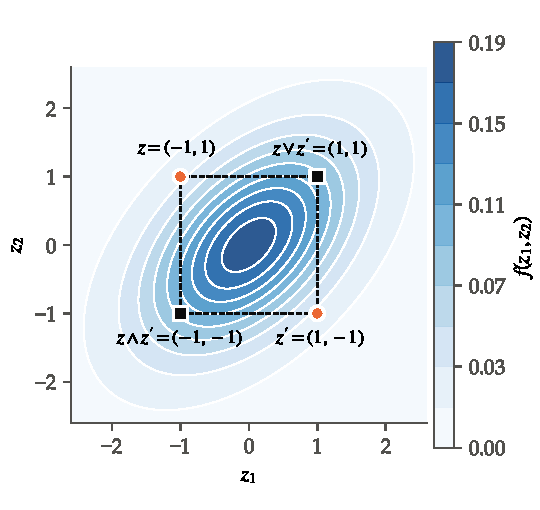
\includegraphics[width=0.56\textwidth]{figures/appB/affiliation.pdf}
\caption{The affiliation inequality for the standard bivariate normal density with correlation $\frac{1}{2}$. The
unordered points $z = (-1, 1)$ and $z' = (1, -1)$ (circles) have join $z \vee z' = (1, 1)$ and meet $z \wedge z' = (-1, -1)$
(squares). The density is $0.09435$ at the join and the meet and $0.02487$ at $z$ and $z'$, so
$f(z \vee z')f(z \wedge z') = 0.00890$ exceeds $f(z)f(z') = 0.000619$, by the factor $e^{\frac{8}{3}} \approx 14.39$.}
\label{fig:B-affiliation}
\end{figure}

\begin{remark}[The general definition]\label{rem:B-affil-general}
\citet[Appendix]{MilgromWeber1982} define affiliation without densities. A set $A \subseteq \R^k$ is \emph{increasing} if its
indicator is nondecreasing, and a set $S$ is a sublattice if $z \vee z', z \wedge z' \in S$ whenever $z, z' \in S$. The variables
are \emph{associated} if $\Pr(Z \in A \cap A') \geq \Pr(Z \in A)\Pr(Z \in A')$ for all increasing sets $A$ and $A'$. They are
affiliated if they are associated conditional on every sublattice $S$ of positive probability. Their Theorem 24
shows that, for variables with a density, this is equivalent to \eqref{eq:B-affil} almost everywhere.
\end{remark}

\begin{proposition}[Characterization, \citealp{MilgromWeber1982}, Theorem 1]\label{prop:B-affil-char}
\leavevmode
\begin{enumerate}[label=(\roman*)]
  \item A strictly positive, twice continuously differentiable density $f$ on a product of intervals is affiliated if
  and only if $\frac{\partial^2\ln f}{\partial z_l\,\partial z_m} \geq 0$ for all $l \neq m$.
  \item If $f = g_1g_2$ with $g_1$ and $g_2$ nonnegative functions that satisfy \eqref{eq:B-affil}, then $f$ is affiliated.
\end{enumerate}
\end{proposition}

\Cref{prop:14-affil-char} proves both parts. Part (i) is also \cref{prop:B-smooth-supermod} applied to $\ln f$, and
\citet[p.~1098]{MilgromWeber1982} cite \citet[p.~310]{Topkis1978} for it. Part (ii) multiplies the inequalities
for $g_1$ and $g_2$, which is legitimate because all terms are nonnegative.

For two variables, affiliation is a statement about conditional densities, and it feeds directly into the chain of
stochastic orders.

\begin{proposition}[Affiliation, MLRP and dominance]\label{prop:B-affil-mlrp}
Let $(X, Z)$ have a strictly positive density $f(x, z)$ on a rectangle, with conditional density $f(x \mid z)$ and
conditional CDF $F(x \mid z)$.
\begin{enumerate}[label=(\roman*)]
  \item $(X, Z)$ is affiliated if and only if $f(x \mid z)$ has the MLRP in $z$: for $z' > z$, $\frac{f(x \mid z')}{f(x \mid z)}$ is
  nondecreasing in $x$.
  \item Let $(X, Z)$ be affiliated and $z' > z$. The conditional distribution given $z'$ dominates the one given $z$ in
  the reverse hazard rate and hazard rate orders. In particular, $\Pr(X \geq x \mid Z = z)$ is nondecreasing in $z$.
  \item If $(X, Z)$ is affiliated, then $\E[\varphi(X) \mid Z = z]$ is nondecreasing in $z$ for every nondecreasing $\varphi$.
\end{enumerate}
\end{proposition}

\begin{proof}
(i) For $x' > x$ and $z' > z$, inequality \eqref{eq:B-affil} reads $f(x', z')f(x, z) \geq f(x, z')f(x', z)$. Dividing by the
product of the marginal densities of $Z$ at $z$ and $z'$ turns joint densities into conditional ones, and dividing
again by $f(x' \mid z)f(x \mid z) > 0$ gives
$\frac{f(x' \mid z')}{f(x' \mid z)} \geq \frac{f(x \mid z')}{f(x \mid z)}$, the MLRP. Each step reverses
\citep[footnote 16]{MilgromWeber1982}. Parts (ii) and (iii) follow from part (i) by \cref{prop:B-orders-chain} and
\cref{prop:B-fosd-expectations}, applied to $X_B \sim F(\cdot \mid z')$ and $X_A \sim F(\cdot \mid z)$.
\end{proof}

Part (ii) follows from the affiliation that \citet{CampoPerrigneVuong2003} assume in their asymmetric affiliated
private values model, so that $\Pr(V_1 \geq v \mid V_2 = v_2)$ is nondecreasing in $v_2$. \Cref{ch:auction-theory}
proves the same chain in the auction notation. Milgrom and Weber derive the properties that auction theory needs
from affiliation.

\begin{proposition}[Properties of affiliated variables, \citealp{MilgromWeber1982}, Theorems 2--5]\label{prop:B-affil-properties}
Let $Z = (Z_1, \dots, Z_k)$ be affiliated.
\begin{enumerate}[label=(\roman*)]
  \item (Order statistics.) Suppose the density $f(s, x_1, \dots, x_n)$ of a common component $s$ and signals $x_i$ is
  affiliated and symmetric in $(x_2, \dots, x_n)$. Let $Y_1 \geq \dots \geq Y_{n-1}$ be the order statistics of
  $(X_2, \dots, X_n)$. Then $(S, X_1, Y_1, \dots, Y_{n-1})$ is affiliated.
  \item (Monotone transformations.) If $g_1, \dots, g_k$ are all nondecreasing or all nonincreasing, then
  $g_1(Z_1), \dots, g_k(Z_k)$ are affiliated.
  \item (Subvectors.) $Z_1, \dots, Z_{k-1}$ are affiliated.
  \item (Conditional expectations.) For any nondecreasing $H$, the function
  $h(a_1, b_1; \dots; a_k, b_k) = \E[H(Z) \mid a_1 \leq Z_1 \leq b_1, \dots, a_k \leq Z_k \leq b_k]$ is nondecreasing in all its arguments.
  In particular, $\E[H(Z) \mid Z_1 = z_1, \dots, Z_l = z_l]$ is nondecreasing in $(z_1, \dots, z_l)$.
\end{enumerate}
\end{proposition}

\begin{proof}[Proofs and sketches]
(i) The joint density of $(S, X_1, Y_1, \dots, Y_{n-1})$ is
\[
  (n - 1)!\,f(s, x_1, y_1, \dots, y_{n-1})\,\indic\{y_1 \geq y_2 \geq \dots \geq y_{n-1}\}
\]
\citep[eq.~(4), p.~1099]{MilgromWeber1982}. The set of ordered vectors is a lattice, because componentwise maxima
and minima of two decreasing sequences are decreasing. Its indicator therefore satisfies \eqref{eq:B-affil}. The
product rule of \cref{prop:B-affil-char}(ii) gives the result.

(ii) We prove the case of strictly increasing, differentiable $g_l$. By the change-of-variables formula, the density
of $W = (g_1(Z_1), \dots, g_k(Z_k))$ is
\[
  f_W(w) = f\bigl(g_1^{-1}(w_1), \dots, g_k^{-1}(w_k)\bigr)\prod_{l=1}^k\frac{1}{g_l'(g_l^{-1}(w_l))}.
\]
The map $w \mapsto (g_1^{-1}(w_1), \dots, g_k^{-1}(w_k))$ is increasing coordinate by coordinate, so it commutes with joins and
meets. The first factor therefore satisfies \eqref{eq:B-affil}. The product is a product of functions of one
coordinate each, which satisfies \eqref{eq:B-affil} with equality. \Cref{prop:B-affil-char}(ii) completes the
argument. If all $g_l$ are decreasing, joins and meets swap, and \eqref{eq:B-affil} is symmetric in them.

(iii) Write $Z = (U, W)$ with $U = (Z_1, \dots, Z_{k-1})$ and $W = Z_k$, and let $f(u, w)$ be the joint density. Fix
$u, u' \in \R^{k-1}$. We must show that the marginal $\int f(u, w)\,\dd w$ satisfies \eqref{eq:B-affil}, that is,
\[
  \int f(u \vee u', w)\,\dd w\int f(u \wedge u', w)\,\dd w \geq \int f(u, w)\,\dd w\int f(u', w)\,\dd w.
\]
Write each product as a double integral over $(w, w')$ and fold the region $w > w'$ onto $w < w'$. For $w < w'$ define
\begin{align*}
  \Theta_1 &= f(u \vee u', w)f(u \wedge u', w'), & \Theta_2 &= f(u \vee u', w')f(u \wedge u', w),\\
  \Xi_1 &= f(u, w)f(u', w'), & \Xi_2 &= f(u, w')f(u', w).
\end{align*}
The left side is the integral of $\Theta_1 + \Theta_2$ and the right side the integral of $\Xi_1 + \Xi_2$ over $w < w'$, so it
suffices to show $\Theta_1 + \Theta_2 \geq \Xi_1 + \Xi_2$ pointwise. Affiliation of $f$ gives $\Theta_2 \geq \Xi_1$ and $\Theta_2 \geq \Xi_2$,
because in both cases the join of the two arguments is $(u \vee u', w')$ and the meet is $(u \wedge u', w)$. Affiliation in $u$
at fixed $w$ and at fixed $w'$ gives, after multiplying, $\Theta_1\Theta_2 \geq \Xi_1\Xi_2$. Now
$(\Theta_2 - \Xi_1)(\Theta_2 - \Xi_2) \geq 0$ expands to
\[
  \Theta_2(\Xi_1 + \Xi_2) \leq \Theta_2^2 + \Xi_1\Xi_2 \leq \Theta_2^2 + \Theta_1\Theta_2.
\]
Dividing by $\Theta_2 > 0$ gives the claim. If $\Theta_2 = 0$, then $\Xi_1 = \Xi_2 = 0$ and the claim is trivial. This is the
simplest case of the composition results of \citet{KarlinRinott1980}.

(iv) We prove the bivariate case $k = 2$, $l = 1$. Write $\E[H(Z_1, Z_2) \mid Z_1 = z_1] = \E[H(z_1, Z_2) \mid Z_1 = z_1]$. Raising
$z_1$ raises the integrand $H(z_1, \cdot)$ pointwise, and it shifts the conditional distribution of $Z_2$ up in the sense of
first-order dominance (\cref{prop:B-affil-mlrp}). By \cref{prop:B-fosd-expectations} both effects raise the
conditional expectation. \citet[Appendix]{MilgromWeber1982} derive the general statement from the conditional
covariance inequality below.
\end{proof}

Affiliation implies a covariance inequality that is often easier to use than the density condition.

\begin{theorem}[Association, \citealp{MilgromWeber1982}, Theorems 22--23]\label{thm:B-association}
If $Z$ is affiliated, then for every pair of nondecreasing functions $g$ and $h$ and every sublattice $S$ of positive
probability,
\[
  \E[g(Z)h(Z) \mid S] \geq \E[g(Z) \mid S]\,\E[h(Z) \mid S].
\]
With $S = \R^k$, affiliated variables are \emph{associated}: $\Cov(g(Z), h(Z)) \geq 0$. Moreover,
$\E[g(Z) \mid A] \geq \E[g(Z)] \geq \E[g(Z) \mid A^c]$ for every increasing set $A$ of positive probability.
\end{theorem}

\begin{proof}[Proof for one variable]
Let $k = 1$ and let $Z'$ be an independent copy of $Z$. Because $g$ and $h$ are both nondecreasing, $g(Z) - g(Z')$ and
$h(Z) - h(Z')$ have the same sign, so
\[
  0 \leq \E\bigl[(g(Z) - g(Z'))(h(Z) - h(Z'))\bigr] = 2\E[g(Z)h(Z)] - 2\E[g(Z)]\E[h(Z)].
\]
This is Chebyshev's covariance inequality. For general $k$, the inequality for indicators of increasing sets is
association, which is part of Milgrom and Weber's general definition of affiliation (\cref{rem:B-affil-general}).
Their Theorem 24 shows that a density satisfying \eqref{eq:B-affil} is affiliated in that sense. The step functions
$g_m(z) = \frac{1}{m}\sum_{i \geq 1}\indic\{g(z) > \frac{i}{m}\}$ are sums of indicators of increasing sets and approximate a
nonnegative nondecreasing $g$, which extends the inequality from indicators to functions
\citep[Theorems 22--23]{MilgromWeber1982}. Conditioning on a sublattice $S$ multiplies the density by the indicator
of $S$, which satisfies \eqref{eq:B-affil}, so the conditional density is again affiliated.
\end{proof}

Taking $g$ and $h$ to be coordinate functions shows that affiliated variables are nonnegatively correlated. The
converse fails badly, as the examples show.

\begin{example}[Affiliated and non-affiliated densities]\label{ex:B-affil-examples}
\leavevmode
\begin{enumerate}[label=(\alph*)]
  \item \emph{Independence.} A product of marginal densities satisfies \eqref{eq:B-affil} with equality.
  \item \emph{Normal vectors.} Let $Z \sim N(\mu, \Sigma)$. Then $\ln f(z) = \text{const} - \frac{1}{2}(z - \mu)^\T\Sigma^{-1}(z - \mu)$, and
  $\frac{\partial^2\ln f}{\partial z_l\,\partial z_m} = -(\Sigma^{-1})_{lm}$. By \cref{prop:B-affil-char}(i), $Z$ is affiliated if and only if
  every off-diagonal element of the precision matrix $\Sigma^{-1}$ is nonpositive. In the bivariate case with standard
  deviations $\sigma_1$, $\sigma_2$ and correlation $\rho_{12}$ (written with a subscript to distinguish it from
  pass-through),
  \[
    \ln f = \text{const} - \frac{1}{2(1 - \rho_{12}^2)}\left[\frac{(z_1 - \mu_1)^2}{\sigma_1^2} - \frac{2\rho_{12}(z_1 - \mu_1)(z_2 - \mu_2)}{\sigma_1\sigma_2} + \frac{(z_2 - \mu_2)^2}{\sigma_2^2}\right],
  \]
  so $\frac{\partial^2\ln f}{\partial z_1\,\partial z_2} = \frac{\rho_{12}}{(1 - \rho_{12}^2)\sigma_1\sigma_2}$. A bivariate normal vector is affiliated
  if and only if $\rho_{12} \geq 0$. With three or more variables, nonnegative correlations do not suffice. The
  covariance matrix with unit variances and correlations $\Corr(Z_1, Z_2) = \Corr(Z_1, Z_3) = \frac{1}{2}$ and
  $\Corr(Z_2, Z_3) = 0$ is positive definite, but its inverse has $(\Sigma^{-1})_{23} = \frac{1}{2} > 0$. Conditional on $Z_1$, the
  variables $Z_2$ and $Z_3$ are negatively related, and the vector is not affiliated.
  \item \emph{Farlie-Gumbel-Morgenstern density.} On $[0, 1]^2$ let $c(z_1, z_2) = 1 + \vartheta(1 - 2z_1)(1 - 2z_2)$ with
  $|\vartheta| \leq 1$. It integrates to one, has uniform marginals, and $\Cov(Z_1, Z_2) = \frac{\vartheta}{36}$, so
  $\Corr(Z_1, Z_2) = \frac{\vartheta}{3}$. Its partial derivatives are $c_1 = -2\vartheta(1 - 2z_2)$, $c_2 = -2\vartheta(1 - 2z_1)$
  and $c_{12} = 4\vartheta$. Hence
  \[
    \frac{\partial^2\ln c}{\partial z_1\,\partial z_2} = \frac{c\,c_{12} - c_1c_2}{c^2}
    = \frac{4\vartheta\bigl[1 + \vartheta(1 - 2z_1)(1 - 2z_2)\bigr] - 4\vartheta^2(1 - 2z_1)(1 - 2z_2)}{c^2} = \frac{4\vartheta}{c^2}.
  \]
  The density is affiliated if and only if $\vartheta \geq 0$.
  \item \emph{Mineral rights.} Let the common value $V$ have density $h$, and let signals be $S_i = V + \epsilon_i$ with
  $\epsilon_1, \dots, \epsilon_n$ i.i.d., independent of $V$, with a log-concave density $f_\epsilon$. The conditional density of a
  signal is $f_\epsilon(s - v)$. For $v' > v$, write $t = s - v$ and $d = v' - v > 0$. Then
  \[
    \ln\frac{f_\epsilon(s - v')}{f_\epsilon(s - v)} = \ln f_\epsilon(t - d) - \ln f_\epsilon(t),
  \]
  which is nondecreasing in $t$, and hence in $s$, because the increments of the concave function $\ln f_\epsilon$ shrink as its
  argument grows. The MLRP holds. Each factor $f_\epsilon(s_i - v)$ of the joint density
  $h(v)\prod_{i=1}^n f_\epsilon(s_i - v)$ satisfies \eqref{eq:B-affil} in $(v, s_i)$, and therefore on the whole vector, since
  joins and meets act coordinate by coordinate. By \cref{prop:B-affil-char}(ii), $(V, S_1, \dots, S_n)$ is affiliated
  \citep[p.~1099]{MilgromWeber1982}. Normal, logistic and Gumbel noise all qualify (\cref{tab:B-logconcave}).
\end{enumerate}
\end{example}

\Cref{fig:B-affiliation} illustrates \eqref{eq:B-affil} for a bivariate normal density with correlation
$\frac{1}{2}$. The points $z = (-1, 1)$ and $z' = (1, -1)$ are unordered, and their join $(1, 1)$ and meet $(-1, -1)$ lie
along the direction of positive dependence, where the density is higher.

In auction theory these tools combine as follows. By \cref{prop:B-affil-properties}(i) and (iv), the expected value
$\E[V_1 \mid X_1 = x, Y_1 = y]$ is nondecreasing in both arguments, which makes symmetric equilibrium bids increasing.
By part (iv) with the upper bound on $Y_1$ lowered, $\E[V_1 \mid X_1 = x, Y_1 < x] \leq \E[V_1 \mid X_1 = x]$, which is the winner's
curse. \Cref{ch:auction-theory} develops both, and \cref{ch:auction-empirics} uses affiliation in the
identification of affiliated private values.

The first-order condition of a symmetric first-price auction with affiliated private values shows where
the conditional distributions enter. Let $B_1$ be the highest bid among bidder 1's rivals. Let
$G_{B_1|b_1}$ and $g_{B_1|b_1}$ be its distribution and density conditional on bidder 1's own bid.
\citet[eq.~4, p.~175]{LiPerrigneVuong2002} show that the equilibrium condition is equivalent to
\begin{equation*}
v = b + \frac{G_{B_1|b_1}(b \mid b)}{g_{B_1|b_1}(b \mid b)} .
\end{equation*}
Each value is therefore a known function of its bid and of the joint distribution of bids, which the data
reveal \citep[Section~3.1, eq.~3.1]{AtheyHaile2007}. Under independence the conditioning on $b_1$ drops out.
Under affiliation it stays, because a high own bid signals high rival bids. Bids inherit affiliation from
values, since the equilibrium bid function is increasing (\cref{prop:B-affil-properties}(ii)).
\citet[Proposition~1, p.~175]{LiPerrigneVuong2002} characterize the bid distributions that such a model can
generate. A distribution qualifies if and only if it is symmetric and affiliated and the right side above is
strictly increasing in $b$.


\section{Bibliographic notes}\label{sec:B-notes}

Optimization, comparative statics and duality are covered in every graduate text in microeconomic theory.
\citet{MasColellWhinstonGreen1995} prove the Kuhn-Tucker conditions, the theorem of the maximum and the duality
results of \cref{sec:B-duality}. \citet{SimonBlume1994} give the matrix and calculus background.
\citet{MilgromSegal2002} prove the envelope theorem for arbitrary choice sets, which is the version that mechanism
design and auction theory need. \citet{Samuelson1947} introduced the correspondence principle and the Le Chatelier
principle into economics. \citet{DeatonMuellbauer1980b} develop duality for demand analysis at book length. Their
chapters on rationing, aggregation and index numbers supply the shadow prices, representative incomes and
cost-of-living bounds of \cref{sec:B-welfare}. \citet{Hausman1981} showed how to recover exact welfare measures from
an estimated demand curve.
\citet{BulowPfleiderer1983} and \citet{WeylFabinger2013} are the main references on pass-through and the curvature
of demand.

The extreme value foundations of discrete choice are due to \citet{McFadden1974, McFadden1978, McFadden1981}, and
the survey of \citet{McFadden1984} collects them. \citet{SmallRosen1981} derived the log-sum measure of consumer
surplus, and \citet{Williams1977} and \citet{DalyZachary1978} proved that the expected maximum utility has the choice
probabilities as its gradient. \citet{AndersonDePalmaThisse1992} connect discrete choice with representative-consumer
models of product differentiation. \citet{Train2009} is the standard text on discrete choice with simulation.
\citet{Cardell1997} constructed the distribution behind the random-coefficients reading of the nested logit, and
\citet{McFaddenTrain2000} showed that mixed logits approximate any random utility model.

\citet{David1981} and \citet{ArnoldBalakrishnanNagaraja1992} are the standard references on order statistics.
\citet{AtheyHaile2002, AtheyHaile2007} turned these results into a theory of identification for auctions, and the
deconvolution lemma of \citet{Kotlarski1966} underlies the treatment of unobserved auction heterogeneity. On fixed
points, \citet{StokeyLucas1989} treat contractions in function spaces, and \citet{Judd1998} discusses the numerical
side. \citet{Berry1994} proved that market shares can be inverted for mean utilities, and
\citet{BerryLevinsohnPakes1995} supplied the contraction that computes the inverse. \citet{BerryGandhiHaile2013}
established invertibility under much weaker conditions. \citet{BerryPakes2007} show how far the contraction weakens when the logit error
vanishes. Chapter~11 of \citet{Tirole1988} is a compact guide to the equilibrium concepts of the book, and its
Section~11.6.1 derives their existence from the theorem of \citet{Debreu1952}. \citet{DasguptaMaskin1986} treat
games with discontinuous payoffs.

Log-concavity entered economics from probability theory. \citet{Prekopa1971} and \citet{Borell1975} proved the
integration results, and \citet{CaplinNalebuff1991} used them to prove the existence of price equilibrium in
differentiated-products oligopoly. \citet{BagnoliBergstrom2005} classify the common distributions. Lattice methods
for comparative statics begin with \citet{Topkis1978}, and \citet{MilgromShannon1994} found their ordinal form.
\citet{Topkis1979}, \citet{Vives1990} and \citet{MilgromRoberts1990} developed the theory of supermodular games, and
\citet{Vives1999} applies it to oligopoly. \citet{BulowGeanakoplosKlemperer1985} introduced strategic substitutes
and complements. \citet{NockeSchutz2018} develop the aggregative structure of logit and CES pricing games, and
\citet[p.~229]{AskerNocke2021} survey its use in merger analysis. \citet{MilgromWeber1982} made affiliation the central dependence concept of auction
theory, and \citet{LiPerrigneVuong2002} turned it into a nonparametric estimator for first-price auctions.
\citet{KarlinRinott1980} study the same property under the name of multivariate total positivity, and
\citet{ShakedShanthikumar2007} cover the stochastic orders of \cref{sec:B-stochastic-orders}.

\section{Exercises}\label{sec:B-exercises}

\begin{enumerate}[label=\arabic*., leftmargin=*, itemsep=6pt]

\item \emph{Duality with CES utility.} Let $U(q_1, q_2) = (q_1^r + q_2^r)^{\frac{1}{r}}$ with $r < 1$ and $r \neq 0$, and
write $\sigma_{\mathrm{CES}} = \frac{1}{1 - r}$.
\begin{enumerate}[label=(\alph*)]
  \item Derive the Marshallian demands and the indirect utility function. Show that
  $q_i = \frac{p_i^{-\sigma_{\mathrm{CES}}}I}{P^{1 - \sigma_{\mathrm{CES}}}}$ with
  $P^{1 - \sigma_{\mathrm{CES}}} = p_1^{1 - \sigma_{\mathrm{CES}}} + p_2^{1 - \sigma_{\mathrm{CES}}}$.
  \item Derive the expenditure function $e(p, u) = uP$. Verify Shephard's lemma, Roy's identity and the symmetry of
  the Slutsky matrix.
  \item Show that the elasticity of $\frac{h_1}{h_2}$ with respect to $\frac{p_2}{p_1}$ equals $\sigma_{\mathrm{CES}}$.
  \item Use \cref{prop:B-virtual} to show that the compensating variation of removing good 2 is finite when
  $\sigma_{\mathrm{CES}} > 1$ and infinite when $\sigma_{\mathrm{CES}} < 1$. Interpret the difference.
  \item Ration good 1 at $z$ units. Derive the restricted expenditure function $e^*(p, u, z)$ and the shadow price
  $p_1^*(p_2, u, z)$, and verify $\frac{\partial e^*}{\partial z} = p_1 - p_1^*$ (\cref{rem:B-rationing}). With two
  goods the ration fixes $q_2$, so $S^*_{22} = 0$. Use $Sp = 0$ to check that $S_{22} - \frac{S_{21}^2}{S_{11}} = 0$,
  as \cref{rem:B-lechatelier} requires.
\end{enumerate}

\item \emph{Exact welfare from log-linear demand.} Let the demand for good 1 be $q_1 = \exp(c_0 + c_1p_1 + c_2I)$ with
$c_1 < 0$ and $c_2 > 0$, holding the other prices fixed.
\begin{enumerate}[label=(\alph*)]
  \item Write the differential equation \eqref{eq:B-hausman-ode} for this demand and solve it by separation of
  variables. Use the constant of integration as the utility index.
  \item Derive the indirect utility function and check that Roy's identity returns $q_1$.
  \item Derive the compensating variation of a price increase from $p_1^0$ to $p_1^1$. Show that it tends to the
  change in Marshallian consumer surplus as $c_2 \to 0$.
  \item Show that the Hicksian demand is positive at every finite price, so the virtual price is infinite. Is the
  value of the good still finite? Compare with the linear demand of \cref{ex:B-hausman-linear}.
  \item For a rise in $p_1$ alone, show that the bounds \eqref{eq:B-cv-ev-bounds} follow from the fact that
  compensated demand slopes down. Compute both bounds and both exact measures for $c_0 = 1$, $c_1 = -1$,
  $c_2 = 0.01$, $I = 100$ and a price rise from 1 to 2.
\end{enumerate}

\item \emph{Pass-through and conduct.} Consider the supply relation \eqref{eq:B-supply-relation}.
\begin{enumerate}[label=(\alph*)]
  \item Derive \eqref{eq:B-pt-conduct} step by step, with $\varepsilon_S$ defined relative to marginal cost including
  the tax.
  \item Show that a pass-through rate of one is consistent with three worlds: price taking with flat marginal cost,
  monopoly with exponential demand, and monopoly with log-convex demand and rising marginal cost.
  \item Let $P(Q) = a - bQ$ and $mc(Q) = c + dQ$ with $b, d > 0$. Show that $\rho = \frac{1}{1 + \theta + \frac{d}{b}}$,
  first from the proposition and then by solving the model directly.
  \item Explain what these results imply for tests of market power that regress prices on taxes.
\end{enumerate}

\item \emph{Cournot comparative statics.} Let $N$ symmetric firms with constant marginal cost $c$ face inverse demand
$P(Q)$, and treat $N$ as a continuous variable.
\begin{enumerate}[label=(\alph*)]
  \item Write the symmetric equilibrium condition $P(Nq) + qP'(Nq) = c$. Use the implicit function theorem to derive
  $\frac{\dd q}{\dd N}$ and $\frac{\dd Q}{\dd N}$.
  \item State conditions on $P'$ and $P''$ under which $\frac{\dd Q}{\dd N} > 0$ and $\frac{\dd q}{\dd N} < 0$. Relate
  the second inequality, business stealing, to the sign of $P' + qP''$.
  \item Use the envelope theorem to derive $\frac{\dd \pi}{\dd N}$ and show that it is negative under the conditions
  of part (b).
  \item Verify all three derivatives for linear demand $P(Q) = A - Q$.
\end{enumerate}

\item \emph{Extreme value algebra.} Let $\epsilon_{i0}, \dots, \epsilon_{iJ}$ be independent standard Gumbel shocks and
$u_{ij} = \delta_j + \epsilon_{ij}$.
\begin{enumerate}[label=(\alph*)]
  \item Prove max-stability for $\mathrm{EV}(0, b)$ shocks and use it to derive the logit shares with scale $b$.
  \item Show that the expected maximal utility conditional on choosing $j$ is the same for every $j$. Derive
  $\E[\epsilon_{ij} \mid j \text{ chosen}] = \gamma_E - \ln s_j$.
  \item In a nested logit with one nest of $m$ identical products of mean utility $\delta$ and an outside good,
  compute expected consumer surplus as a function of $m$ and $\sigma$. Show that it grows like
  $\frac{1 - \sigma}{\alpha}\ln m$ for large $m$, and explain the role of $\sigma$.
  \item Derive the within-nest correlation $1 - (1 - \sigma)^2$ from Cardell's representation.
\end{enumerate}

\item \emph{Order statistics and competing risks.}
\begin{enumerate}[label=(\alph*)]
  \item Let $n$ values be drawn independently from $F(x) = x^a$ on $[0, 1]$ with $a > 0$. Derive the CDF and the mean
  of the second-highest value. Check your answer against \cref{cor:B-os-revenue} at $a = 1$.
  \item Prove the recurrence relation \eqref{eq:B-os-recurrence} for $k = n - 1$ directly from \eqref{eq:B-os-cdf},
  for i.i.d.\ draws.
  \item Two independent bidders have values with $F_i(x) = x^{a_i}$ on $[0, 1]$, $i = 1, 2$. Compute
  $G_1^w(x) = \Pr(M \leq x, I = 1)$ and the CDF of the maximum $M$. Verify that \eqref{eq:B-competing-risks}
  recovers $F_1$.
  \item In part (c), show that the winning value and the identity of the winner are independent. Explain why the
  frequency of wins then carries all the information that separates the two distributions.
\end{enumerate}

\item \emph{Contractions and equilibrium computation.}
\begin{enumerate}[label=(\alph*)]
  \item In the plain logit, show that the Jacobian of the share-inversion map \eqref{eq:B-blp-map} is $\mathbf{1}s^\T$.
  Compute the number of iterations needed per digit of accuracy when $s_0 = 0.05$ and when $s_0 = 0.5$.
  \item Take a nested logit with one nest of two products. Show that the undampened map has a Jacobian eigenvalue
  $-\frac{\sigma}{1 - \sigma}$, and that the dampened map \eqref{eq:B-nl-dampened} sends this eigenvalue to zero.
  \item A single-product logit monopolist has $\alpha = 1$ and $v = \tilde\delta - \alpha mc = 3$. Use
  \cref{prop:B-logit-br} to compute its share. Show that the markup iteration \eqref{eq:B-markup-iteration} diverges
  locally while best-response iteration converges in one step.
  \item Use \eqref{eq:B-iterations} to bound the number of iterations that reach a tolerance of $10^{-8}$ from an
  initial step of $10$, for $\kappa = 0.9$ and $\kappa = 0.99$.
\end{enumerate}

\item \emph{Log-concavity, supermodularity and affiliation.}
\begin{enumerate}[label=(\alph*)]
  \item Show that the standard logistic density is log-concave. Deduce that its hazard rate is nondecreasing and
  that values with this distribution satisfy Myerson's regularity condition.
  \item Show that the single-product logit pricing game is log-supermodular. Use \cref{thm:B-smgames} to show that
  an increase in one firm's marginal cost does not lower any equilibrium price. Then use the closed-form best
  response \eqref{eq:B-logit-br-closed} to show that every price strictly rises.
  \item Verify that the Farlie-Gumbel-Morgenstern density of \cref{ex:B-affil-examples} is affiliated if and only if
  $\vartheta \geq 0$. Show directly that affiliation implies the monotone likelihood ratio property for this
  density.
  \item Prove that the likelihood ratio order implies first-order stochastic dominance. Give an example of two
  distributions ranked by first-order dominance but not by the likelihood ratio.
\end{enumerate}

\end{enumerate}
